%% For double-blind review submission, w/o CCS and ACM Reference (max submission space)
\documentclass[acmsmall,review,anonymous,screen]{acmart}\settopmatter{printfolios=true,printccs=false,printacmref=true}
%% For double-blind review submission, w/ CCS and ACM Reference
%\documentclass[acmsmall,review,anonymous]{acmart}\settopmatter{printfolios=true}
%% For single-blind review submission, w/o CCS and ACM Reference (max submission space)
%\documentclass[acmsmall,review]{acmart}\settopmatter{printfolios=true,printccs=false,printacmref=false}
%% For single-blind review submission, w/ CCS and ACM Reference
%\documentclass[acmsmall,review]{acmart}\settopmatter{printfolios=true}
%% For final camera-ready submission, w/ required CCS and ACM Reference
%\documentclass[acmsmall]{acmart}\settopmatter{}


%% Journal information
%% Supplied to authors by publisher for camera-ready submission;
%% use defaults for review submission.
\acmJournal{PACMPL}
\acmVolume{1}
\acmNumber{POPL} % CONF = POPL or ICFP or OOPSLA
\acmArticle{1}
\acmYear{2023}
\acmMonth{1}
\acmDOI{} % \acmDOI{10.1145/nnnnnnn.nnnnnnn}
\startPage{1}

%% Copyright information
%% Supplied to authors (based on authors' rights management selection;
%% see authors.acm.org) by publisher for camera-ready submission;
%% use 'none' for review submission.
\setcopyright{none}
%\setcopyright{acmcopyright}
%\setcopyright{acmlicensed}
%\setcopyright{rightsretained}
%\copyrightyear{2018}           %% If different from \acmYear

%% Bibliography style
\bibliographystyle{ACM-Reference-Format}
%% Citation style
%% Note: author/year citations are required for papers published as an
%% issue of PACMPL.
\citestyle{acmauthoryear}   %% For author/year citations


%%%%%%%%%%%%%%%%%%%%%%%%%%%%%%%%%%%%%%%%%%%%%%%%%%%%%%%%%%%%%%%%%%%%%%
%% Note: Authors migrating a paper from PACMPL format to traditional
%% SIGPLAN proceedings format must update the '\documentclass' and
%% topmatter commands above; see 'acmart-sigplanproc-template.tex'.
%%%%%%%%%%%%%%%%%%%%%%%%%%%%%%%%%%%%%%%%%%%%%%%%%%%%%%%%%%%%%%%%%%%%%%


%% Some recommended packages.
\usepackage{booktabs}   %% For formal tables:
                        %% http://ctan.org/pkg/booktabs
\usepackage{subcaption} %% For complex figures with subfigures/subcaptions
                        %% http://ctan.org/pkg/subcaption

\usepackage{tikz}
\usetikzlibrary{arrows}


%% MY STUFF
\usepackage{preamble}
\usepackage{pifont}

% \addbibresource{my_biblio.bib} % do not put this in preamble or it breakes automatic suggestions for citations in vscode

% % macros
\usepackage{select_version}
\usepackage{my_macro}
\usepackage{laetitia_macro}
\usepackage{etienne_macros}

\begin{document}

%% Title information
\title{A non-sequential hierarchy of message-passing models}
        %% [Short Title] is optional;
                                        %% when present, will be used in
                                        %% header instead of Full Title.
%\titlenote{with title note}             %% \titlenote is optional;
                                        %% can be repeated if necessary;
                                        %% contents suppressed with 'anonymous'
%\subtitle{Subtitles}                     %% \subtitle is optional
%\subtitlenote{with subtitle note}       %% \subtitlenote is optional;
                                        %% can be repeated if necessary;
                                        %% contents suppressed with 'anonymous'


%% Author information
%% Contents and number of authors suppressed with 'anonymous'.
%% Each author should be introduced by \author, followed by
%% \authornote (optional), \orcid (optional), \affiliation, and
%% \email.
%% An author may have multiple affiliations and/or emails; repeat the
%% appropriate command.
%% Many elements are not rendered, but should be provided for metadata
%% extraction tools.

%% Author with single affiliation.
\author{Cinzia Di Giusto}
%\authornote{with author1 note}          %% \authornote is optional;
                                        %% can be repeated if necessary
\orcid{nnnn-nnnn-nnnn-nnnn}             %% \orcid is optional
\affiliation{
%  \position{Position1}
%  \department{Department1}              %% \department is recommended
  \institution{Institution1}            %% \institution is required
  \streetaddress{Street1 Address1}
  \city{City1}
  \state{State1}
  \postcode{Post-Code1}
  \country{Country1}                    %% \country is recommended
}
\email{first1.last1@inst1.edu}          %% \email is recommended

%% Author with two affiliations and emails.
\author{Davide Ferré}
%\authornote{with author2 note}          %% \authornote is optional;
                                        %% can be repeated if necessary
\orcid{nnnn-nnnn-nnnn-nnnn}             %% \orcid is optional
\affiliation{
  \position{Position2a}
  \department{Department2a}             %% \department is recommended
  \institution{Institution2a}           %% \institution is required
  \streetaddress{Street2a Address2a}
  \city{City2a}
  \state{State2a}
  \postcode{Post-Code2a}
  \country{Country2a}                   %% \country is recommended
}
\email{first2.last2@inst2a.com}         %% \email is recommended
       %% \email is recommended

%% Author with two affiliations and emails.
\author{Laetitia Laversa}
%\authornote{with author2 note}          %% \authornote is optional;
                                        %% can be repeated if necessary
\orcid{nnnn-nnnn-nnnn-nnnn}             %% \orcid is optional
\affiliation{
  \position{Position2a}
  \department{Department2a}             %% \department is recommended
  \institution{Institution2a}           %% \institution is required
  \streetaddress{Street2a Address2a}
  \city{City2a}
  \state{State2a}
  \postcode{Post-Code2a}
  \country{Country2a}                   %% \country is recommended
}
\email{first2.last2@inst2a.com}         %% \email is recommended
       %% \email is recommended


\author{Etienne Lozes}
%\authornote{with author2 note}          %% \authornote is optional;
                                        %% can be repeated if necessary
\orcid{nnnn-nnnn-nnnn-nnnn}             %% \orcid is optional
\affiliation{
  \position{Position2a}
  \department{Department2a}             %% \department is recommended
  \institution{Institution2a}           %% \institution is required
  \streetaddress{Street2a Address2a}
  \city{City2a}
  \state{State2a}
  \postcode{Post-Code2a}
  \country{Country2a}                   %% \country is recommended
}
\email{first2.last2@inst2a.com}



%% Abstract
%% Note: \begin{abstract}...\end{abstract} environment must come
%% before \maketitle command
\begin{abstract}
There is a wide variety of message-passing communication models ranging from synchronous "rendez-vous" 
communications to fully asynchronous/out-of-order communications. For large-scale distributed systems, the
communication model is determined by the transport layer of the network, and a few classes of 
orders of message delivery (FIFO, causally ordered) have been identified in the early days of 
distributed computing. For local-scale message-passing applications, 
e.g., running on a single machine, the communication model may be determined by the actual implementation of 
message buffers and how FIFO queues are used. While large-scale communication
models, such as causal ordering, are defined by logical axioms, local-scale models are often defined by an operational
semantics. In this work, we connect these two approaches, and we present a unified hierarchy of communication
models encompassing both large-scale and local-scale models, based on their non-sequential behaviours.
We also show that all the communication models we consider can be axiomatised in the monadic second order logic, 
and may therefore benefit from several bounded verification techniques based on bounded special treewidth.

\end{abstract}


%% 2012 ACM Computing Classification System (CSS) concepts
%% Generate at 'http://dl.acm.org/ccs/ccs.cfm'.
\begin{CCSXML}
<ccs2012>
<concept>
<concept_id>10011007.10011006.10011008</concept_id>
<concept_desc>Software and its engineering~General programming languages</concept_desc>
<concept_significance>500</concept_significance>
</concept>
<concept>
<concept_id>10003456.10003457.10003521.10003525</concept_id>
<concept_desc>Social and professional topics~History of programming languages</concept_desc>
<concept_significance>300</concept_significance>
</concept>
</ccs2012>
\end{CCSXML}

\ccsdesc[500]{Software and its engineering~General programming languages}
\ccsdesc[300]{Social and professional topics~History of programming languages}
%% End of generated code


%% Keywords
%% comma separated list
\keywords{keyword1, keyword2, keyword3}  %% \keywords are mandatory in final camera-ready submission


%% \maketitle
%% Note: \maketitle command must come after title commands, author
%% commands, abstract environment, Computing Classification System
%% environment and commands, and keywords command.
\maketitle

\section{Introduction}
% \begin{itemize}
%   \item Interleaving based semantics VS partial order/graph based semantics
%   \item Synchronous and asynchronous communication
%   \item The problem of synchronizability
% \end{itemize}



% !TEX root = ../popl-paper.tex
Reasoning about distributed message-passing applications is  hard. The degree of asynchrony
of the communication model is  an important ingredient of the application.
One reason
is that the communication architecture on which the application runs may vary, and must be accurately specified. In particular, an under-approximated communication model may hide safety errors,
such as unspecified receipts, whereas an over-approximated model may hide deadlocks. 

In synchronous communication (also known as rendez-vous communication), send and receive events are viewed as
a single event, i.e., a receive event and the corresponding send event happen simultaneously. The idea behind asynchronous communication, instead, is to decouple send and receive events, so that a receive event can happen indefinitely after the corresponding send event. By introducing some additional constraints on the execution of those events, we can obtain new communication models that sit somewhere between synchronous and fully asynchronous communication.
In this paper we try to clarify and classify some of these communication models.
%We consider only point-to-point communication, that is, messages that have exactly one sender and one receiver.
On  one hand, we consider communication models that were proposed in the early days of large-scale distributed computing to establish the correctness of some distributed algorithms, such as \emph{causal ordering}~\cite{Lamport78} for the correctness of Lamport's distributed mutual exclusion algorithm (see also~\cite{Renesse93}), or the weaker "FIFO" peer-to-peer assumption. On the other hand, we look at communication models that emerge
naturally when considering local-scale message-passing applications, which are based on predictable
message buffering supported by local FIFO queues (for instance "mailboxes"). Such communication models have
been considered in more recent works (for instance in~\cite{DBLP:journals/tcs/BasuB16}) and have caused
some confusion, specifically regarding the difference between causal ordering and mailboxes~\cite{DBLP:conf/cav/BouajjaniEJQ18,DBLP:conf/fossacs/GiustoLL20}.

The classification and axiomatisation of large-scale communication models received great attention in the late 90s~\cite{DBLP:journals/dc/Charron-BostMT96}, while the local-scale communication models have only started to be investigated quite recently by Chavrou~\emph{et al.}~\cite{DBLP:journals/fac/ChevrouHQ16}, focusing on a \emph{sequential} view of the behaviours of message-passing
applications (to be detailed below).
At the same time, several works~\cite{KraglQH18,GleissenthallKB19,DBLP:conf/cav/BouajjaniEJQ18,DBLP:conf/cav/LangeY19} recently addressed the verification of
asynchronous message-passing applications by reduction to their synchronous semantics (see also~\cite{Lipton75} for a seminal work on these questions). These results strongly rely on the ability to safely approximate an asynchronous communication model with a synchronous one. There is therefore a need to clarify how the synchronous-asynchronous spectrum of communication models is organised.

In this work, we start from the sequential hierarchy established by Chevrou~\emph{et al.}~\cite{DBLP:journals/fac/ChevrouHQ16}, where a
communication model is represented by a class of sequential executions; we revisit this hierarchy
with a non-sequential point of view: we define a communication model as a class of
\emph{Message Sequence Charts} (MSCs in the following).
Our MSCs are a graphical representation of computations of distributed systems, and they are a simplified
version of the ITU recommendation~\cite{messagesequencecharts}.
Roughly speaking, a distributed system is composed by a set of
sequential processes that can exchange messages. Each process executes a sequence of \emph{events}, which in our case will be either \emph{send}
or \emph{receive} events. A send event $s$ and a receive event $r$ are said to be \emph{matching} if the message sent by $s$ is the same  that is
received by $r$. 
A distributed computation is the \\
\noindent
concurrent execution of each process. In an MSC, such as the one in Fig.~\ref{fig:msc_ex}, each
vertical line is called a \emph{process line} and it represents the order in which events are executed by a single process, with time running from
top to bottom; arrows are used to represent messages and they connect a send event with the corresponding matching receive.
Given a message $m_i$, we will use $!i$ and $?i$ to denote the corresponding matching send and receive events, respectively. A single process line defines a
total order over the events executed by that process, i.e., an event $e$ happens before another event $e'$ if $e$ is higher in the process line;
in Fig.~\ref{fig:msc_ex}, if we look at process $q$ we see that $?1$ happens before $?2$. However, in general MSCs only specify a partial order
over events. Consider the events $!1$ and $!2$ in Fig.~\ref{fig:msc_ex}, which are executed by two different processes; these two events are \emph{truly concurrent}, in the sense that this MSC does not tell us which one is executed first.

\begin{wrapfigure}{r}{0pt}
	\begin{tikzpicture}[scale=0.8, every node/.style={transform shape}]
		\newproc{0}{p}{-2.5};
		\newproc{1}{q}{-2.5};
		\newproc{2}{r}{-2.5};

		\newmsgm{0}{1}{-0.5}{-0.5}{1}{0.5}{black};
		\newmsgm{2}{1}{-1.2}{-1.2}{2}{0.5}{black};
		\newmsgm{1}{0}{-1.9}{-1.9}{3}{0.5}{black};

		\newflechehorinverse{Purple}{-1.2}{2}{1};
		\newflechevert{Purple}{1}{-1.3}{-2.0};
		\newflechehorinverse{Purple}{-1.9}{1}{0};

		\newevent{black}{0}{-0.5}{!1}{left};
		\newevent{black}{1}{-0.5}{?1}{right};
		\newevent{black}{2}{-1.2}{!2}{right};
		\newevent{black}{1}{-1.2}{?2}{left};
		\newevent{black}{1}{-1.9}{!3}{below right};
		\newevent{black}{0}{-1.9}{?3}{left};

	\end{tikzpicture}
	\captionof{figure}{Red arrows between $!2$ and $?3$ denote a causal path.}
	\label{fig:msc_ex}
\end{wrapfigure}

\noindent Even though events on different processes can be concurrent, this is not always the case. For instance, a send event must always happen
before the matching receive event. Graphically, this \emph{happens before} relation between events on different processes is represented
by a path that follows the direction of the arrows and runs from top to bottom. This will be referred to as a \emph{causal path}, because it
estabilishes a causal relation between events. Fig.~\ref{fig:msc_ex} shows an example of causal path between the events $!2$ and $?3$. 
% Consider events $!1$ and $?2$ of the MSC shown in Fig.~\ref{fig:msc_ex}. Even though they are executed by different processes, $?2$ must happen
% before $!1$ because $?2$ must be executed after $!2$, which happens before $?1$, which in turn happens before $!1$.
% The fact that $!1$ is higher on his own process line compared to $!2$ does not meaning anything with respect to the order in which they are
% executed.


% Since an MSC defines a partial order over the events of a distributed system, it can always be extended to a total order, which will be referred to as a \emph{linearization}.
% %Given an MSC, it can have multiple linearizations. For the MSC in Fig.~\g:msc_ex}, both $!1\;?1\;!2\;?2$ and $!2\;!1\;?1\;?2$ are valid linearizations, i.e. a total order over the events which is compatible with the partial order defined by the MSC.
% Intuitively, a linearization represents the order in which events are executed by the distributed system according to \emph{absolute time}, i.e. as they are seen by an external viewer that has a global view of all the processes.




As mentioned before, in this work we interpret communication models as classes of MSCs.
This non-sequential view of the communication models is arguably the "standard one",
rather than the sequential point of view adopted by Chevrou~\emph{et al}. It is more relevant for comparing communication models, as some
of them, such as causally ordered communications, intrinsically rely on this non-sequential view and the happens-before relation. Large-scale communication models are quite easy to axiomatize in a formal language, such as monadic second order logic (MSO) over MSCs. Local-scale
communication models, on the other hand, are easy to define by means of an operational semantics involving FIFO queues, but their axiomatization
in MSO is error prone and requires particular attention. The choice of MSO as a specification language for the axiomatisation of
these communication models is not incidental: there is a wealth of results on MSO model-checking over MSCs that originated from
the work of Genest~\emph{et al.}~\cite{genest2004kleene,GKM07}, with recent developments by Bollig~\emph{et al.} in the context
of synchronisability~\cite{BolligGFLLS21}.

\etienne{Do we really want to repeat Fig2 at Fig8? By the way Fig2 is not the up to date version of Fig8}

Our contributions are the following:
\begin{itemize}
	\item We review the peer-to-peer FIFO, causally ordered, mailbox, \onen, \nn, asynchronous, and synchronous communication models
	and propose definitions of these models in terms of classes of MSCs. For the communication models whose intuition stems from
	an operational semantics, we provide an alternative operational definition, and we show soundness and completeness.

	\item From these definitions, we deduce a new non-sequential hierarchy of communication models (see Fig.~\ref{fig:msc_hierarchy_full})
	and establish the strictness of this hierarchy by means of several examples.
	Surprisingly, the \onen class, that could be thought of as the "dual" of the mailbox class, is a subclass of mailbox class. This strongly
	contrasts with Chevrou~\emph{et al.} sequential hierarchy, where \onen and mailbox are incomparable. The comparison between
	the \onen and mailbox classes is non-trivial in our non-sequential setting, and it motivates the introduction
	of several technical alternative characterisations of these communication models.

	\item We show that all of these communication models can be axiomatised in MSO. This result is rather subtle for mailbox and \onen, and highly non-trivial for \nn. For the latter, we develop a constructive proof based on an
	algorithm that computes a \nn linearisation of an MSC.

	\item Building on the MSO characterization of these communication models, we derive several new decidability results (cfr. Fig. \ref{fig:stw-boundshort}) for bounded
	model-checking of systems of communicating finite state machines under various bounded assumptions (existential boundedness, weak synchronisability, etc).
\end{itemize}



\begin{figure}[t]
	\captionsetup[subfigure]{justification=centering}
	% \centering
%	
	\begin{subfigure}{0.3\textwidth}\centering	
	\begin{tikzpicture}[scale=0.78, every node/.style={transform shape}]
		\draw  (0,0) rectangle (1.5,.6);
		\draw (1.5,0.3) node[left]{\rsc};
		\draw  (0,0) rectangle (2.1,1.2);
		\draw (2.1,0.9) node[left]{\nn};
		\draw  (0,0) rectangle (2.7,1.8);
		\draw (2.7,1.5) node[left]{\onen};
		\draw  (0,0) rectangle (3.3,2.4);
		\draw (3.3,2.1) node[left]{\mb};
		\draw  (0,0) rectangle (3.9,3);
		\draw (3.9,2.7) node[left]{\co};
		\draw  (0,0) rectangle (4.5,3.6);
		\draw (4.5,3.3) node[left]{\pp};
		\draw  (0,0) rectangle (5.1,4.2);
		\draw (5.1,3.9) node[left]{\asy};
	\end{tikzpicture}
	\caption{The hierarchy of MSC classes.\\ ~}
	\label{fig:msc_hierarchy_full}
	\end{subfigure} \quad   
	\begin{subfigure}{0.65\textwidth}\centering
	{\small
		\begin{tabular}{| c | c | c|  c| c| } 
			\hline
			& Weakly  & Weakly  & $\exists$k & $\forall$k  \\
			& sync & k-sync & bounded & bounded \\
			\hline \hline
			$\asy$ &  \xmark & \cmark & \cmark & \cmark \\
			\hline
			$\oneone$  & \xmark~[1] & \cmark~[1] & \cmark~[1] & \cmark~[1] \\
			\hline
			$\co$  & \xmark & \cmark & \cmark & \cmark \\
			\hline
			$\none$ & \cmark~[1] & \cmark~[1] & \cmark~[1] & \cmark~[1] \\
			\hline
			$\onen$ & \cmark & \cmark & \cmark & \cmark \\
			\hline
			$\nn$ & \cmark & \cmark & \cmark & \cmark \\
			\hline
		%	$\rsc$ & \cmark & \cmark & \cmark & \cmark & \cmark \\
		%	\hline
		\end{tabular}
		}
		\caption{ (Un)decidability results for the synchronisability problems, %(each 
		%combination of a communication model $\comsymb$ and a class $\aMSCclass$ of MSCs is a different 
		%synchronisability problem). 
		%The symbol \xmark\;stands for undecidability and unbounded special tree-width
	%	of $\comsymb\cap \aMSCclass$, whereas \cmark\;stands for decidability and bounded STW
%		of $\comsymb\cap \aMSCclass$.  
		[1] indicates that the result was shown in \cite{BolligGFLLS21}.}
		\label{fig:stw-boundshort}
\end{subfigure}
\caption{Main contributions}
	%\etienne{Maybe move that figure later? end of section 2? section 6?}
\end{figure}

\paragraph{\bf Outline} The paper is organized as follows. Section~\ref{sec:MSC} describes the communication models we consider. We also recall the notion of MSC and introduce formal definitions for these models, seen as classes of MSCs.
In Section~\ref{sec:impl}, we rely on
an operational semantics to provide an alternative definition for some of these communication models, which we prove to be sound and complete.
Section~\ref{sec:MSO} characterizes the classes of MSCs via MSO logic.
In Section~\ref{sec:hierarchy}, we compare all of the considered communication models and show our main result: a strict non-sequential hierarchy of communication models.
Finally, Section~\ref{sec:checking} shows some (un)decidability results for various bounded model-checking
problems based on MSO and on the notion of special treewidth.


%\hrule
%
%\bigskip
%
%\etienne{Below: keep in the intro, move elsewhere, or drop}
%
%Consider the events $!1$ and $!2$ in Fig.~\ref{fig:msc_ex}, which are executed by two different processes; these two events are said to be \emph{concurrent}, in the sense that this MSC does not tell us which one is executed first.
%
%generalize the models to  consider unmatched messages (i.e., messages that have been sent, but not yet read).
%MSCs are a graphical representation of the  computations of distributed systems.  Roughly speaking, a distributed system is composed by a set of sequential processes that can exchange messages. Each process exhibits a sequence of \emph{events}, which in our case will be either \emph{send} or \emph{receive} events. A send event $s$ and a receive event $r$ are said to be \emph{matching} if the message sent by $s$ is the same  that is received by $r$. A distributed computation is the concurrent execution of each process. In an MSC, such as the one in Fig.~\ref{fig:msc_ex}, each vertical line is called a \emph{process line} and it represents the order in which events are executed by a single process, with time running from top to bottom; arrows are used to represent messages and they connect a send event with its corresponding matching receive.
%Given a message $m_i$, we will use $!i$ and $?i$ to denote the corresponding two matching send and receive events. A single process line defines a total order over the events executed by that process, i.e., an event $e$ happens before another event $e'$ if $e$ is higher in the process line; in Fig.~\ref{fig:msc_ex}, if we look at process $q$ we see that $?1$ happens before $?2$. However, in general MSCs only specify a partial order over events.
%
%
%\cinzia{Have a look at \url{https://web.archive.org/web/20060826195305/http://www.comp.nus.edu.sg/~thiagu/public_papers/surveymsc.pdf}}
%
%\cinzia{\url{https://link.springer.com/content/pdf/10.1007/978-0-387-35271-8.pdf} to mention while talking about realizability page 81-96}
%
%Going back to our contribution, the work in \cite{DBLP:journals/fac/ChevrouHQ16} describes the properties that a single linearization must satisfy in order to be realizable by a system that uses a given communication model. On the other hand, we are interested in understanding if a given MSC describes a computation that can be realized by a system that uses some communication model $CM$. In other words, given a MSC we want to know if it has at least one linearization that respects the constraints imposed by $CM$. If that is the case, the MSC represents a behaviorthat can be exhibited by a system that uses $CM$ as a communication model. These are two fundamentally dissimilar problems; at the end of this section we provide an example to clarify the difference. In our work, we are going to formally characterize the classes of MSCs which represent valid computations for all of these seven communication models. We also show how these classes form a well-defined hierarchy, which does not correspond entirely to that found in \cite{DBLP:journals/fac/ChevrouHQ16}.

%\cinzia{talk about realizations here?}
%
%\cinzia{say that the two hierarchy differs}
%\paragraph{Contributions.}\cinzia{to rewrite here}
%
%We find of particular interest to study the relation between the classes of MSCs for all of these communication models. For instance, the MSC shown in Fig.~\ref{fig:co_ex} is both asynchronous and $\oneone$, in the sense that we are able to find systems using those communication models that can produce the behaviordescribed by the MSC. Is it always the case than a $\oneone$ MSC is also an asynchronous MSC? What about the other communication models? In Section~\ref{sec:hierarchy} we prove that the classes of MSCs for all these communication models form a very neat hierarchy, which is graphically shown in Fig.~\ref{fig:msc_hierarchy_full}.

% \cinzia{redo fig in tikz}
% \begin{figure}[h]
% 	\centering
% 	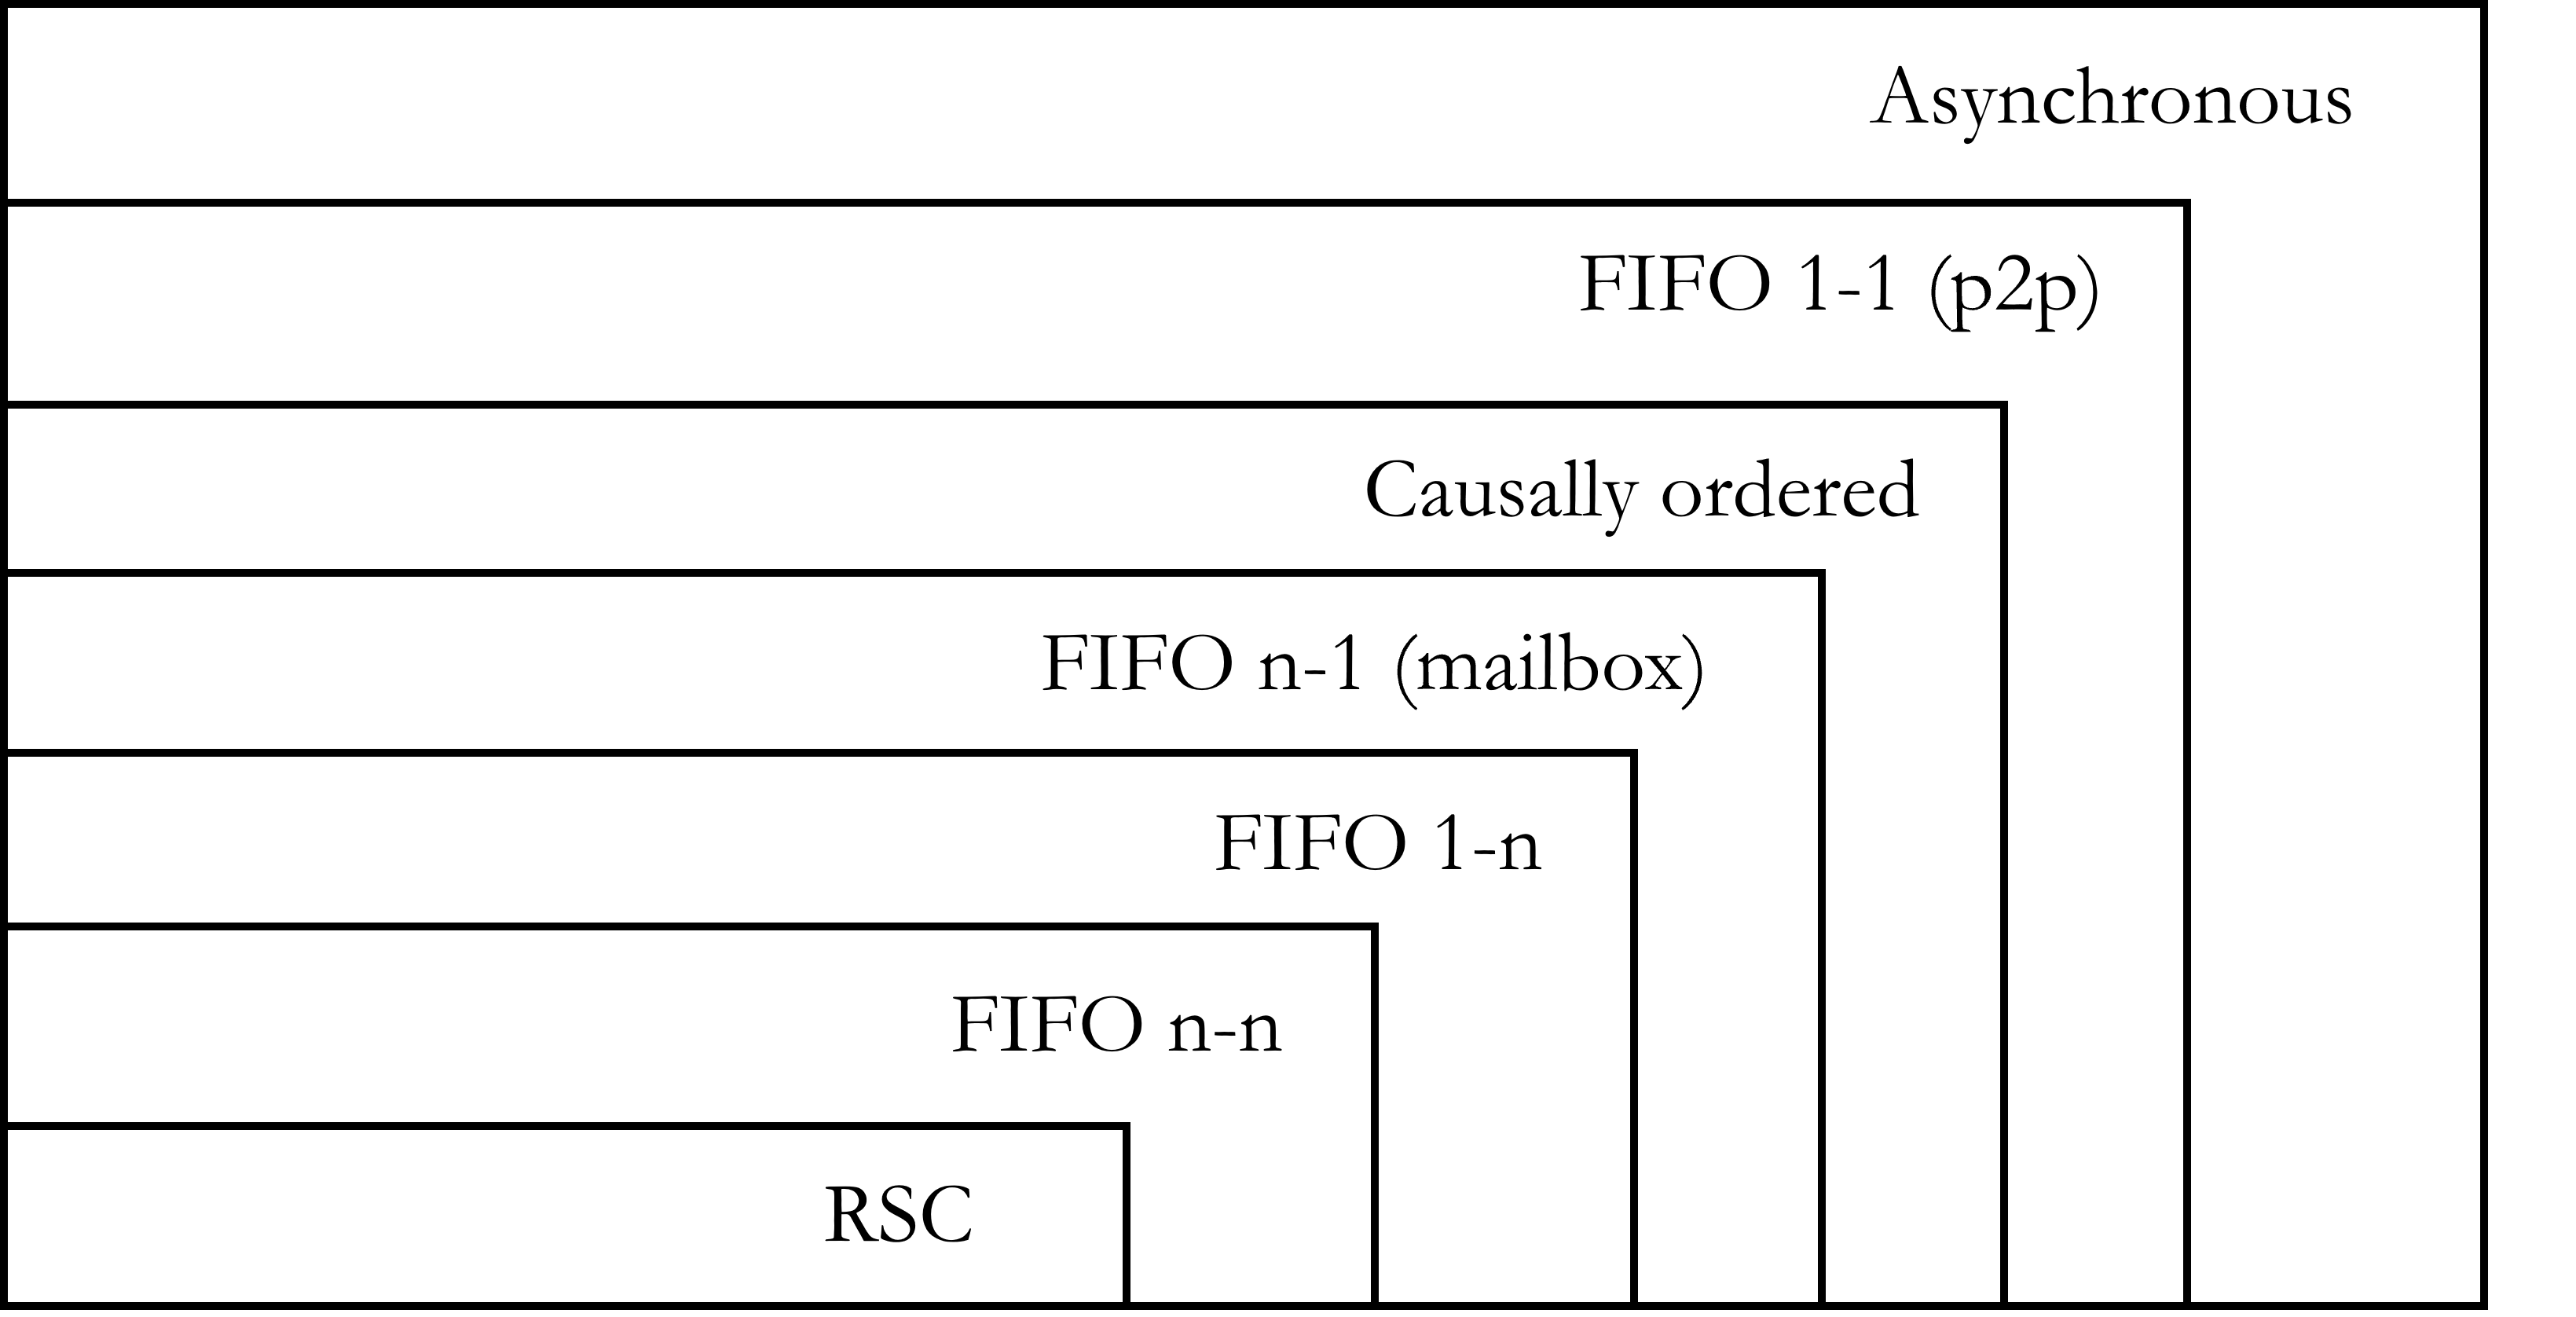
\includegraphics[width=8cm]{msc_hierarchy}
% 	\caption{The hierarchy of MSC classes.}
% 	\label{fig:msc_hierarchy_full}
% \end{figure}





% \section{Asynchronous communication models overview}
% \label{sec:com_models_overview}
% %\begin{itemize}
% %  \item Overview of asynchronous variants
% %  \item High-level description of each variant along with references to implementations (if existing)
% %  \item (Definitions based on linearization, intuitive)
% %  \item (Language of a system with a given communication model as a set of MSCs)
% %  \item Hint of hierarchy result
% %\end{itemize}

% % !TEX root = ../popl-paper.tex

Next, we informally present the communication models we consider. All of them impose different constraints on the order in which messages can be received.
For convenience, we will refer to the system implementing a given communication model with the name of the model. Implementation, or realizations of a communication model are discussed in the following section.
In a similar way, an MSC will be referred with the name of the communication model, since it represents a computation that is valid for that model.

 %In this section, we will present  7 different asynchronous communication models.
%We model a distributed system as a set of concurrent Finite-State Machines (FSMs) that exchange messages asynchronously through channels.
%Each FSM models a single machine/process of the system and transitions are labeled with "send" and "receive" operations, which specify the sender and the receiver of a message. In our work
%The role of the communication model is to impose an order on the reception of messages, according to its specification. For instance, the delivery of a message could be delayed or even prevented by a communication model $CM$, so as to ensure that messages are received in an order that is valid for $CM$. The 7 communication models that we address all impose different constraints on the order in which messages can be received.
%
\paragraph{\bf Fully asynchronous}
In the fully asychronous communication model (\asy) messages can be received at any time once they have been sent, and send events are non-blocking.
%, i.e., the sender of a message does not have to wait for it to be delivered to the recipient, in order to resume normal operations.
\asy systems can be realized (as described in \cite{DBLP:journals/fac/ChevrouHQ16} and \cite{DBLP:journals/tcs/BasuB16})  by a bag where all messages are stored and retrieved when necessary.
This communication model is also referred to as NON-FIFO (cfr.  \cite{DBLP:journals/dc/Charron-BostMT96}).
Fig.~\ref{fig:fully_asy_ex} shows a computation that can be executed by an \asy  system; indeed, even if message $m_1$ is sent before $m_2$, process $q$ does not have to receive $m_1$ first.   We will call $\asMSCs$ the set of all asynchronous MSCs.

\begin{figure}[t]
		\captionsetup[subfigure]{justification=centering}
	% \centering
	\begin{subfigure}[t]{0.2\textwidth}\centering

		\begin{tikzpicture}[scale=0.7, every node/.style={transform shape}]
			\newproc{0}{p}{-2.2};
			\newproc{2}{q}{-2.2};

			\newmsgm{0}{2}{-0.5}{-1.7}{1}{0.1}{black};
			\newmsgm{0}{2}{-1.7}{-0.5}{2}{0.25}{black};

			\end{tikzpicture}
		\caption{Only \asy.}	\label{fig:fully_asy_ex}

		\end{subfigure}
%
%		\begin{subfigure}[t]{0.25\textwidth}
%	\begin{center}
%		\begin{tikzpicture}[scale=0.7, every node/.style={transform shape}]
%			\newproc{0}{p}{-2.2};
%			\newproc{1}{q}{-2.2};
%			\newproc{2}{r}{-2.2};
%
%			\newmsgm{0}{1}{-0.3}{-1.7}{1}{0.1}{black};
%			\newmsgm{0}{2}{-0.7}{-0.7}{2}{0.7}{black};
%			\newmsgm{2}{1}{-1.3}{-1.3}{3}{0.3}{black};
%			\newmsgm{2}{1}{-1.9}{-1.9}{4}{0.3}{black};
%
%			\end{tikzpicture}
%		\caption{A \pp MSC.}
%		\label{fig:pp_ex}
%	\end{center}
%\end{subfigure}
%
	% \centering
	\begin{subfigure}[t]{0.25\textwidth}\centering
		\begin{tikzpicture}[scale=0.7, every node/.style={transform shape}]
			\newproc{0}{p}{-2.2};
			\newproc{1}{q}{-2.2};
			\newproc{2}{r}{-2.2};

			\newmsgm{0}{1}{-0.3}{-1.7}{1}{0.1}{black};
			\newmsgm{0}{2}{-0.9}{-0.9}{2}{0.7}{black};
			\newmsgm{2}{1}{-1.5}{-1.5}{3}{0.3}{black};
			\newmsgm{2}{1}{-2}{-2}{4}{0.3}{black};

			\newflechevert{Purple}{0}{-0.3}{-0.9};
			\newflechehor{Purple}{-0.9}{0}{2};
			\newflechevert{Purple}{2}{-0.9}{-1.5};
		\end{tikzpicture}
		\caption{\asy, \pp, not \co, \\not \mb, not $\onen$, \\not $\nn$, not $\rsc$.} \label{fig:pp_ex}
	\end{subfigure}
	% \hfill
	\begin{subfigure}[t]{0.2\textwidth}\centering
		\begin{tikzpicture}[scale=0.7, every node/.style={transform shape}]
			\newproc{0}{p}{-2.2};
			\newproc{1}{q}{-2.2};
			\newproc{2}{r}{-2.2};

			\newmsgm{0}{2}{-0.3}{-2}{1}{0.1}{black};
			\newmsgm{0}{1}{-1.3}{-1.3}{2}{0.3}{black};
			\newmsgm{2}{1}{-1.5}{-1.5}{3}{0.3}{black};

		\end{tikzpicture}
		\caption{\asy, \pp, \co, \mb, $\onen$, $\nn$, not $\rsc$.}	    \label{fig:co_ex}
	\end{subfigure}
\begin{subfigure}[t]{0.2\textwidth}\centering
	\begin{center}
		\begin{tikzpicture}[scale=0.7, every node/.style={transform shape}]
			\newproc{0}{p}{-2};
			\newproc{1}{q}{-2};
			\newproc{2}{r}{-2};

			\newmsgm{0}{1}{-0.5}{-0.5}{1}{0.3}{black};
			\newmsgm{1}{2}{-1}{-1}{2}{0.3}{black};
			\newmsgm{1}{0}{-1.6}{-1.6}{3}{0.3}{black};

		\end{tikzpicture}
		\caption{Only $\rsc$.}
		\label{fig:rsc_ex}
	\end{center}
\end{subfigure}

		\caption{Examples of MSCs for various communication models.}\label{fig:exmscs}

\end{figure}

\paragraph{\bf Peer-to-peer}
In the peer-to-peer ($\pp$ for short) communication model, any two messages sent from one process to another  are always received in the same order as they were sent. Systems are realized by processes that are  pairwise connected by FIFO channels. %i.e. messages are delivered by channels in the order in which they were sent\footnote{Please note that our definition of Communicating Finite-State Machine is different from the classical one. FIFO channels are replaced by bag channels, which do not ensure any specific order on the delivery of messages.}. This definition of Communicating Finite-State Machines clearly uses the $\oneone$ communication model, since we have FIFO channels between processes that take care of delivering messages in the correct order. The $\oneone$ communication model is referred to as \pp in \cite{DBLP:conf/concur/BolligGFLLS21}.
 \pp systems are also referred to as FIFO $1\mathsf{-}1$ systems as in  \cite{DBLP:journals/fac/ChevrouHQ16} or simply FIFO as in \cite{babaoglu1993consistent, DBLP:journals/dc/Charron-BostMT96, tel2000introduction}).
The MSC shown in Fig.~\ref{fig:fully_asy_ex} is not a $\pp$ MSC; as the receive order of messages $m_1$ and $m_2$  must match the send order.
Fig.~\ref{fig:pp_ex} shows an example of \pp MSC; the only two messages sent by and to the same process are $m_3$ and $m_4$, which are received in the same order  they have been sent. An example of linearization that can be executed by a $\pp$ system is $!1\;!2\;?2\;!3\;!4\;?3\;?1\;?4$. We denote by  $\ppMSCs$  the set of \pp MSCs.




\paragraph{\bf Causally ordered}
In the causally ordered (\co) communication model, messages are delivered to a process according to the causality of their emissions. In other words, if there are two messages $m_1$ and $m_2$ with the same recipient, such that $m_1$ is causally sent before $m_2$ (i.e., there exists a causal path from the first send to the second one), then $m_1$ must be received before $m_2$.
This type of partial order was introduced by Lamport in \cite{lamport2019time} with the "happened before" order. Later, some implementations was proposed in   \cite{kshemkalyani1998necessary, peterson1989preserving} and in \cite{coulouris2005distributed}, where the causal order is called FIFO ordering.
Fig.~\ref{fig:pp_ex}, shows an example of non-causally ordered MSC; there is a causal path between the sending of $m_1$ and $m_3$ (highlighted with red arrows), hence $m_1$ should be received before $m_3$, which is not the case here. On the other hand, Fig.~\ref{fig:co_ex} is \co; note that the only two messages with the same recipient are $m_2$ and $m_3$, but there is no causal path between their respective send events
%(i.e. the causally ordered communication model does not introduce any new constraint that must be satisfied).
 $\coMSCs$ is the set of causally ordered MSCs.


\paragraph{\bf Mailbox}
In the mailbox ($\mb$) communicating model, any two messages sent to a process  must be received in the same order as they have been sent (according to absolute time). Note that these two messages might be sent by different processes and the two send events might be concurrent (i.e., there is no causal path between them). In other words, if a process  receives $m_1$ before $m_2$, then $m_1$ must have been sent before $m_2$. Essentially, $\mb$ coordinates all the senders of a single receiver. For this reason the model is also called FIFO $n\mathsf{-}1$ \cite{DBLP:journals/fac/ChevrouHQ16}.   A high-level implementation of the mailbox communication model could consist in a single incoming FIFO channel for each process, which is shared by all the other processes. A send event would consist in pushing the message on the shared FIFO channel.
A low-level implementation needs a shared real-time clock \cite{cristian1999timed} or a global agreement on event order \cite{defago2004total, raynal2010communication}.
The MSC shown in Fig.~\ref{fig:pp_ex} is not a mailbox MSC; $m_1$ and $m_3$ have the same recipient, but they are not received in the same order as they are sent. The MSC in Fig.~\ref{fig:co_ex} is mailbox; indeed, we are able to find a linearization that respects the mailbox constraints, such as $!1\;!2\;!3\;?2\;?3\;?1$ (note that $m_2$ is both sent and received before $m_3$). Such a linearization will be referred to as a \emph{mailbox linearization}. At this stage, the difference between the class of causally ordered MSCs and the class of mailbox MSCs might not be clear. We will clarify later how all these classes of MSCs are related to each other. Let $\mbMSCs$ be the set of mailbox MSCs.

\paragraph{\bf $\onen$}
The $\onen$ communicating model is the dual of $\none$, it coordinates a sender with all the receivers. Any two messages sent by a process  must be received in the same order (in absolute time) as they are sent. Note that these two messages might be received by different processes and the two receive events might be concurrent.
% In other words, if a process $p$ sends $m_1$ before $m_2$, then $m_1$ must be received before $m_2$ in absolute time.
A high-level implementation of the $\onen$ communication model could consist in a single outgoing FIFO channel for each process, which is shared by all the other processes. A send event would consist in pushing the message on the outgoing FIFO channel.
%As this type of communication is the dual of the $\none$ one, the implementation would require similar tools as above.
The MSC shown in Fig.~\ref{fig:pp_ex} is not a $\onen$ MSC; $m_1$ and $m_2$ are sent in this order by the same process, but they are received in the opposite order (note that there is a causal path between the reception of $m_2$ and the reception of $m_1$, so $?2$ happens before $?1$ in every linearization of this MSC). Fig.~\ref{fig:co_ex} shows an example of $\onen$ MSC; $m_1$ is sent before $m_2$ by the same process, and we are able to find a linearization where $m_1$ is received before $m_2$, such as $!1\;!2\;!3\;?1\;?2\;?3$. Such a linearization will be referred to as a \emph{$\onen$ linearization}. Let $\onenMSCs$ be the set of $\onen$ MSCs.

\paragraph{\bf $\nn$}
In  $\nn$ communicating model, messages are globally ordered and delivered according to  their emission order. Any two messages must be received in the same order as they are sent, in absolute time. Note that these two messages might be received by different processes and the two receive events might be concurrent.
%In other words, if a message $m_1$ is sent before $m_2$ in absolute time, then $m_1$ must be received before $m_2$ in absolute time.
The $\nn$ coordinates all the senders with all the receivers. A high-level implementation of the $\nn$ communication model could consist in a single FIFO channel shared by all processes. It is considered also in \cite{DBLP:journals/tcs/BasuB16} where it is called  many-to-many (denoted $^\ast$-$^\ast$). But, as underlined in \cite{DBLP:journals/fac/ChevrouHQ16}, such an implementation would be inefficient and unrealistic.
 The MSC shown in Fig.~\ref{fig:pp_ex} is clearly not a $\nn$ MSC; if we consider messages $m_1$ and $m_2$ we have that, in every linearization, $!1$ happens before $!2$ and $?2$ happens before $?1$. This violates the constraints imposed by the $\nn$ communication model. The MSC in Fig.~\ref{fig:co_ex} is $\nn$ because we are able to find a linearization that satisfies the $\nn$ constraint, e.g. $!1\;!2\;!3\;?1\;?2\;?3$. Such a linearization will be referred to as an \emph{$\nn$ linearization}.  $\nnMSCs$ is the set of $\nn$ MSCs.

\paragraph{\bf Realizable with Synchronous Communication}
The Realizable with Synchronous Communication ($\rsc$) communication model imposes that a send event is  immediately followed by its corresponding receive event. It was introduced in \cite{DBLP:journals/dc/Charron-BostMT96}. It is the asynchronous model which is the  closest to the synchronous one. % An asynchronous distributed system that implements the $\rsc$ communication model effectively behaves as a synchronous system. 
%The authors of \cite{kshemkalyani2011distributed} propose a strategy to implement RSC executions from a synchronous system.  
Only the MSC shown in Fig.~\ref{fig:rsc_ex} is an example of $\rsc$ MSC; we can easily find a linearization that respects the constraints of the $\rsc$ communication model, such as $!1\;?1\;!2\;?2\;!3\;?3$. Such a linearization will be referred to as an \emph{$\rsc$ linearization}. Let $\rscMSCs$ be the set of $\rsc$ MSCs.



% % \section{Preliminaries}\label{sec:prelim}
% % \begin{itemize}
% %   \item Communicating systems (communicating finite-state automata with bag channels)
% %   \item MSCs and (conflict graph)
% %   \item Causal path
% %   \item Monadic Second-Order logic on MSCs
% %   \item (Language of a system as a set of MSCs)
% %   \item (Model checking and synchronizability)
% % \end{itemize}

% % 
% !TEX root = popl-paper.tex

\subsection{Communicating Systems}

We now recall the definition of communicating systems (aka communicating finite-state
machines or message-passing automata), which consist of finite-state machines $A_p$
(one for every process $p \in \Procs$) that can communicate through channels from $\Ch$. In our case, we consider the most general definition in which channels behave as bags, which means that no specific order is enforced on the delivery of messages.

\begin{definition}\label{def:cs}
A \emph{communicating system} over $\Procs$ and $\Msg$ is a tuple
   $ \Sys = (A_p)_{p\in\procSet}$. For each
   $p \in \Procs$, $A_p = (Loc_p, \delta_p, \ell^0_p)$ is a finite transition system where
   $\Loc_p$ is a finite set of local (control) states, $\delta_p
   \subseteq \Loc_p \times \pAct{p} \times \Loc_p$ is the
   transition relation, and $\ell^0_p \in Loc_p$ is the initial state.
\end{definition}

Given $p \in \Procs$ and a transition $t = (\ell,a,\ell') \in \delta_p$, we let
$\tsource(t) = \ell$, $\ttarget(t) = \ell'$, $\tlabel(t) = a$, and
$\tmessage(t) = \msg$ if $a \in \msAct{\msg} \cup \mrAct{\msg}$.

\smallskip

There are in general two ways to define the semantics of a communicating system.
Most often it is defined as a global infinite transition system that keeps track
of the various local control states and all (unbounded) channel contents.
As, in this paper, our arguments are based on a graph view of MSCs, we will define
the language of $\Sys$ directly as a set of MSCs. These two semantic views are essentially
equivalent, but they have different advantages depending on the context.
We refer to \cite{CyriacG14} for a thorough discussion.

\davidequestion{MSCs are formally defined in chapter 5... maybe move here in the preliminaries just the asynchronous definition?}
Let $\msc = (\Events,\procrel,\lhd,\lambda)$ be an MSC.
A \emph{run} of $\Sys$ on $\msc$ is a mapping
$\rho: \Events \to \bigcup_{p \in \Procs} \delta_p$
that assigns to every event $e$ the transition $\rho(e)$
that is executed at $e$. Thus, we require that
\begin{enumerate*}[label={(\roman*)}]
\item for all $e \in \Events$, we have $\tlabel(\rho(e)) = \lambda(e)$,
\item for all $(e,f) \in {\procrel}$, $\ttarget(\rho(e)) = \tsource(\rho(f))$,
\item for all $(e,f) \in {\lhd}$, $\tmessage(\rho(e)) = \tmessage(\rho(f))$,
and
\item for all $p \in \Procs$ and $e \in \Events_p$ such that there is no $f \in \Events$ with $f \procrel e$, we have $\tsource(\rho(e)) = \ell_p^0$.
\end{enumerate*}

Letting run $\Sys$ directly on MSCs is actually very convenient.
This allows us to associate with $\Sys$ its p2p language and mailbox language
in one go. The \emph{\pp language} of $\Sys$ is $\ppL{\Sys} = \{\msc \in \ppMSCs \mid$ there is a run of $\Sys$ on $\msc\}$.
The \emph{mailbox language} of $\Sys$ is $\mbL{\Sys} = \{\msc \in \mbMSCs \mid$ there is a run of $\Sys$ on $\msc\}$.

Note that, following \cite{DBLP:conf/cav/BouajjaniEJQ18,DBLP:conf/fossacs/GiustoLL20},
we do not consider final states or final configurations, as our purpose is to
reason about all possible
traces that can be \emph{generated} by $\Sys$.
%We will discuss this issue in more detail later in the paper. \todo{Do we still discuss this in the conference version or can we omit this sentence?}
The next lemma is obvious for the p2p semantics and follows from Lemma~\ref{lem:mb-prefix} for
	the mailbox semantics.

\begin{lemma}\label{lem:prefix-closed}
For all $\comsymb \in \{\ppsymb, \mbsymb\}$, $\cL{\Sys}$ is prefix-closed:
$\Pref{\cL{\Sys}} \subseteq \cL{\Sys}$.
\end{lemma}

\begin{example}
	Fig.~\ref{fig:system_weak_univer} depicts $\systemweakuniver = (A_p, A_q, A_r)$ such that MSC $\mscweakuniver$ in Fig.~\ref{fig:msc_weak_univer} belongs to $\ppL{\systemweakuniver}$ and to $\mbL{\systemweakuniver}$.
	There is a unique run $\rho$ of $\systemweakuniver$ on $\mscweakuniver$.
	We can see that $(e_3',e_4) \in {\rightarrow}$ and $\ttarget(\rho(e_3')) = \tsource(\rho(e_4)) = \ell_r^{1}$, $(e_2, e_2') \in \lhd_{\mscweakuniver}$, and $\tmessage(\rho(e_2)) = \tmessage(\rho(e_2')) = \msg_2$.
	\end{example}
	\begin{figure}[t]
	\begin{center}
	  \begin{tikzpicture}[>=stealth,node distance=3.2cm,shorten >=1pt,
		every state/.style={text=black, scale =0.75}, semithick,
		font={\fontsize{8pt}{12}\selectfont},
		scale = 0.9
		]
	  \begin{scope}[->]
		  \node[state,initial,initial text={}] (q0)  {$\ell_p^{0}$};
		  \node[state, right of=q0] (q1)  {$\ell_p^{1}$};
				\node[state, right of=q1] (q2) {$\ell_p^{2}$};
	
			\path (q0) edge node [above] {$\send{p}{q}{\msg_1}$} (q1);
				\path (q1) edge node [above] {$\rec{q}{p}{\msg_2}$}(q2);
			\node[thick] at (-1.1,0) {$A_p$};
	  \end{scope}
	
	  \begin{scope}[->, shift={(7.5,0)}]
		  \node[state,initial,initial text={}] (q0)  {$\ell_q^{0}$};
				\node[state, right of=q0] (q1)  {$\ell_q^{1}$};
				\node[state, below of=q1, node distance = 1.5cm] (q2) {$\ell_q^{2}$};
				\node[state, left of=q2] (q3)  {$\ell_q^{3}$};
	
				\path (q0) edge node [above] {$\send{q}{p}{\msg_2}$} (q1);
				\path (q1) edge node [right] {$\send{q}{r}{\msg_3}$}(q2);
				\path (q2) edge node [above] {$\rec{r}{q}{\msg_4}$} (q3);
				\node[thick] at (-1.1,0) {$A_q$};
	  \end{scope}
	
		\begin{scope}[->, shift={(0,-1.25)} ]
		  \node[state,initial,initial text={}] (q0)  {$\ell_r^{0}$};
				\node[state, right of=q0] (q1)  {$\ell_r^{1}$};
				\node[state, right of=q1] (q2) {$\ell_r^{2}$};
	
				\path (q0) edge node [above] {$\rec{q}{r}{\msg_3}$} (q1);
				\path (q1) edge node [above] {$\send{r}{q}{\msg_4}$}(q2);
				\node[thick] at (-1.1,0) {$A_r$};
	  \end{scope}
	\end{tikzpicture}
	\captionof{figure}{System $\systemweakuniver$}
	\label{fig:system_weak_univer}
	\end{center}
	\end{figure}	

\subsection{Conflict Graph}

\davidequestion{The conflict graph is needed only for some proofs on the cuncur paper. I think it makes sense not to include it here and eventually introduce it later in the MSO-treewidth chapter if we really need it.}

We now recall the notion of a conflict graph associated to an MSC defined in \cite{DBLP:conf/cav/BouajjaniEJQ18}. This graph is used to depict the causal dependencies between message exchanges.  Intuitively, we have a dependency whenever
two messages have a process in common. For instance, an $\xrightarrow{SS}$
dependency between message exchanges $v$ and $v'$ expresses the fact that
$v'$ has been sent after $v$, by the same process. This notion is of interest because it was seen in \cite{DBLP:conf/cav/BouajjaniEJQ18} that the notion of synchronizability in MSCs (which is studied in this paper) can be graphically characterized by the nature of the associated conflict graph.
It is defined in terms of linearizations
in \cite{DBLP:conf/fossacs/GiustoLL20}, but we equivalently express it
directly in terms of MSCs.

\newcommand{\type}{\tau}
\newcommand{\stype}{S}
\newcommand{\rtype}{R}
\newcommand{\mexch}{\mu}
\newcommand{\Edges}{\mathit{Edges}}
\newcommand{\Nodes}{\mathit{Nodes}}

For an MSC $\msc = (\Events, \rightarrow, \lhd, \lambda)$ and
$e \in \Events$, we define the type $\type(e) \in \{\stype,\rtype\}$ of $e$ by $\type(e) = \stype$ if $e \in \SendEv{\msc}$
and $\type(e) = \rtype$ if $e \in \RecEv{\msc}$.
Moreover, for $e \in \Unm{\msc}$, we let $\mexch(e) = e$,
and for $(e,e') \in \lhd$, we let $\mexch(e) = \mexch(e') = (e,e')$.


\begin{definition}[Conflict graph]
	The \emph{conflict graph} $\cgraph{\msc}$ of an MSC $\msc = (\Events, \rightarrow, \lhd, \lambda)$ is the labeled graph $(\Nodes, \Edges)$, with $\Edges \subseteq \Nodes \times \{\stype,\rtype\}^2 \times \Nodes$, defined by
	$\Nodes = {\lhd} \cup \Unm{\msc}$ and $\Edges = \{(\mu(e),\type(e)\type(f),\mu(f)) \mid (e,f) \in {\to^+}\}$.
In particular, a node of $\cgraph{\msc}$ is either a single unmatched send event or a message pair $(e,e') \in {\lhd}$.
\end{definition}	

\subsection{Logic and Special treewidth}

\davidequestion{Special treewidth is used only in the final chapter, to me it makes more sense to introduce it there}

\paragraph*{Monadic Second-Order Logic.}
The set of MSO formulas over MSCs (over $\Procs$ and $\Msg$) is given by the grammar
$
\phi ::= x \procrel y \mid x \lhd y \mid \lambda(x) = a \mid x = y \mid x \in X \mid \exists x.\phi \mid \exists X.\phi \mid \phi \vee \phi \mid \neg \phi
$,
where $a \in \Act$, $x$ and $y$ are first-order variables, interpreted as
events of an MSC, and $X$ is a second-order variable, interpreted
as a set of events. We assume that we have an infinite supply of variables,
and we use common abbreviations such as $\wedge$, $\forall$, etc.
The satisfaction relation is defined in the standard way and self-explanatory.
For example, the formula $\neg\exists x.(\bigvee_{a \in \sAct} \lambda(x) = a \;\wedge\; \neg \mathit{matched}(x))$
with $\mathit{matched}(x) = \exists y.x \lhd y$
says that there are no unmatched send events.
It is not satisfied by  MSC $\mscweakuniver$
of Fig.~\ref{fig:msc_weak_univer},
as message $\msg_1$ is not received,
but by $\mscstrongexist$ from Fig.~\ref{fig:msc_strong_exist}.

Given a sentence $\phi$, i.e., a formula without free variables,
we let $L(\phi)$ denote the set of (p2p) MSCs that satisfy $\phi$.
%
It is worth mentioning that the (reflexive) transitive closure of
a binary relation defined by an MSO formula with free variables $x$ and $y$,
such as $x \procrel y$, is MSO-definable so that the logic can freely
use formulas of the form $x \procrel^+ y$ or $x \le y$ (where $\le$
is interpreted as $\le$ for the given MSC $\msc$).
Therefore, the definition of a mailbox MSC can be readily translated into
the formula $\mbformula = \neg \exists x.\exists y.(\neg (x = y) \wedge x \mbpartial y \wedge y \mbpartial x)$ so that we have $L(\mbformula) = \mbMSCs$.
Here, $x \mbpartial y$ is obtained as the MSO-definable reflexive transitive closure of
the union of the MSO-definable relations $\procrel$, $\lhd$, and $\sqsubset$.
In particular, we may define $x \sqsubset y$ by :
\[
x \sqsubset y =
\displaystyle
\hspace{-1em}\bigvee_{\substack{q \in \Procs\\a,b \in \qsAct{q}}}\hspace{-1em}
\lambda(x) = a \;\wedge\; \lambda(y) = b
\wedge
\left(
\begin{array}{rl}
& \mathit{matched}(x) \wedge \neg \mathit{matched}(y)\\[1ex]
\vee & \exists x'.\exists y'. (x \lhd x' \;\wedge\; y \lhd y' \;\wedge\; x' \procrel^+ y')
\end{array}
\right)
\]

\paragraph*{Special treewidth.}

\emph{Special treewidth} \cite{Courcelle10},
is a graph measure that indicates how close
a graph is to a tree (we may also use classical
	\emph{treewidth} instead).
This or similar measures are commonly employed in verification. For instance, treewidth and split-width have been used in \cite{MadhusudanP11} and, respectively, \cite{DBLP:conf/concur/CyriacGK12,AiswaryaGK14} to reason about graph behaviors generated by pushdown and queue systems.
%Here we apply it to reason about MSCs.
There are several ways to define the special treewidth of an MSC.
We adopt the following game-based definition from \cite{DBLP:journals/corr/abs-1904-06942}.

Adam and Eve play a two-player turn based "decomposition game"
whose positions
are MSCs with some pebbles placed on some events.
More precisely, Eve's positions are
\emph{marked MSC fragments} $(M, U)$, where
$\msc = (\Events, \procrel, \lhd, \lambda)$
is an \emph{MSC fragment} (an MSC with possibly some edges from
$\lhd$ or $\to$ removed)
 and $U \subseteq \Events$ is the subset of marked events.
Adam's positions are pairs of marked MSC fragments.
A move by Eve consists in the following steps:
\begin{enumerate}
	\item marking some events of the MSC resulting in $(M, U')$ with $U \subseteq U' \subseteq \Events$,
	\item removing (process and/or message) edges whose endpoints are marked,
	\item dividing $(M, U)$ in $(M_1, U_1)$ and $(M_2, U_2)$ such that $M$ is the disjoint (unconnected) union of $M_1$ and $M_2$
	and marked nodes are inherited.
\end{enumerate}
When it is Adam's turn, he simply chooses one of the two marked MSC fragments.
The initial position is $(\msc,\emptyset)$ where $M$ is the (complete) MSC at hand. A terminal position is any position belonging to Eve such that all events are marked.
%
For $k \in \N$, we say that the game is $k$-winning for Eve if she has a (positional) strategy that allows her,
starting in the initial position and independently of Adam's moves, to reach a terminal position such that, in every single position visited along the play, there are at most $k+1$ marked events.

\newcommand{\CS}[2]{\mathsf{CS}_{(#1,#2)}}
\newcommand{\MSO}[2]{\mathsf{MSO}_{(#1,#2)}}
\newcommand{\LCPDL}[2]{\mathsf{LCPDL}_{(#1,#2)}}
\newcommand{\MSCpm}[2]{\mathsf{MSC}_{(#1,#2)}}
\newcommand{\mbMSCpm}[2]{\mathsf{MSC}_{(#1,#2)}^{\mathsf{mb}}}


\begin{fact}[\cite{DBLP:journals/corr/abs-1904-06942}]
	The special treewidth of an MSC is the least $k$ such that
	the associated game is $k$-winning for Eve.
\end{fact}

The set of MSCs whose special treewidth is at most $k$ is denoted by $\stwMSCs{k}$.

\section{Asynchronous communication models as classes of MSCs}\label{sec:MSC}

% !TEX root = ../popl-paper.tex

In this section, we give both informal descriptions and formal definitions of the communication models that will be considered in the paper. All of them impose different constraints on the order in which messages can be received.
% Implementations, or realizations, of these communication models are discussed in the following section. For convenience, we will refer to a system implementing a given communication model $\comsymb$ as a $\comsymb$-system.
% Similarly, an MSC that represents a valid computation for a communication model $\comsymb$ will be called a $\comsymb$-MSC.

 %In this section, we will present  seven different asynchronous communication models.
%We model a distributed system as a set of concurrent Finite-State Machines (FSMs) that exchange messages asynchronously through channels.
%Each FSM models a single machine/process of the system and transitions are labeled with "send" and "receive" operations, which specify the sender and the receiver of a message. In our work
%The role of the communication model is to impose an order on the reception of messages, according to its specification. For instance, the delivery of a message could be delayed or even prevented by a communication model $CM$, so as to ensure that messages are received in an order that is valid for $CM$. The seven communication models that we address all impose different constraints on the order in which messages can be received.
%

We will use the following customary conventions:  $\abinrel^+$ denotes the transitive closure of a binary relation $\abinrel$, while $\abinrel^*$ denotes the transitive and reflexive closure. When $R^*$ is denoted by a symbol suggesting 
a partial order, like $\leq$, we write e.g. 
$<$ for $R^+$.  The cardinality of a set $A$ is  $\cardinalof{A}$.
%
%\paragraph*{Processes, messages, and actions}
We assume a finite set of \emph{processes} $\Procs=\{p,q,\ldots\}$ and a finite set of message contents (or just "message") $\Msg=\{\msg,\ldots\}$.
Each process may either (asynchronously) send a message to another one, or wait until it receives a message.
We therefore consider two kinds of actions. A \emph{send action} is of the form $\sact{p}{q}{\msg}$;
it is executed by process $p$ and sends message $\msg$ to process $q$.
The corresponding \emph{receive action} executed by $q$ is $\ract{p}{q}{\msg}$.
%
We write $\pqsAct{p}{q}$ to denote the set $\{\sact{p}{q}{\msg} \mid \msg \in \Msg\}$, and
$\pqrAct{p}{q}$ for the set $\{\ract{p}{q}{\msg} \mid \msg \in \Msg\}$.
Similarly, for $p \in \Procs$, we set
$\psAct{p} = \{\sact{p}{q}{\msg} \mid q \in \Procs
% Etienne: shall we forbid processes to send messages to themselves?
%\setminus \{p\}
\}$ and $\msg \in \Msg\}$, etc.
Moreover, $\pAct{p} = \psAct{p} \cup \qrAct{p}$ denotes the set of all actions that are
executed by $p$, and $\Act = \bigcup_{p \in \Procs} \pAct{p}$
is the set of all the actions. When $p$ and $q$
are clear from the context, we may write $!m_i$,
or $!i$ (resp. $?m_i$, $?i$) instead of $\sact{p}{q}{m_i}$ (resp. $\ract{p}{q}{m_i}$).
%\davide{Should we specify somewhere how the notations $"send(,,)"$ and $!i$ (same for receive) are related? I suppose they could confuse the reader, since we basically use them interchangeably in the paper. Also, the difference between action and event is not very clear IMO.}


\paragraph{\bf Fully asynchronous communication}
In the fully asynchronous communication model (\asy), messages can be received at any time once they have been sent, and send events are non-blocking.
%, i.e., the sender of a message does not have to wait for it to be delivered to the recipient, in order to resume normal operations.
It can be modeled as a bag where all messages are stored and retrieved by processes when necessary (as described in \cite{DBLP:journals/fac/ChevrouHQ16} and \cite{DBLP:journals/tcs/BasuB16}).
It is also referred to as NON-FIFO (cfr.  \cite{DBLP:journals/dc/Charron-BostMT96}).
An MSC that shows a valid computation for the fully asynchronous communication model will be called a fully asynchronous MSC (or simply MSC). An example of such an MSC can be found in Fig.~\ref{fig:fully_asy_ex}; indeed, even if message $m_1$ is sent before $m_2$, process $q$ does not have to receive $m_1$ first. Below, we give the formal definition of MSC.

\begin{definition}[MSC]\label{def:msc}
	An {MSC}  over $\Procs$ and $\Msg$ is a tuple $\msc = (\Events,\procrel,\lhd,\lambda)$, where 
	$\Events$ is a finite (possibly empty) set of \emph{events}, $\lambda: \Events \to \Act$ is a labelling 
	function that associates an action to each event,
	and $\procrel,\lhd$ are binary relations on $\Events$ that satisfy the following three conditions.
	For $p \in \Procs$, let $\Events_p = \{e \in \Events \mid \lambda(e) \in \pAct{p}\}$ be 
	the set of events that are executed by $p$. 
	\begin{enumerate}
		\item The \emph{process relation} $\procrel\subseteq \Events \times \Events$ 
		relates an event to its immediate successor on
		the same process:
		$\procrel=\bigcup_{p \in \Procs} \procrel_p$ for some 
		relations ${\procrel_p} \subseteq \Events_p \times \Events_p$ such that $\procrel_p$ is 
		the direct successor relation of a total order on $\Events_p$.  
		\item The \emph{message relation} ${\lhd} \subseteq \Events \times \Events$ 
		relates pairs of matching send/receive events: 	
		\begin{enumerate}%\itemsep=0.5ex
			\item[(2a)] for every pair $(e,f) \in {\lhd}$, there are processes two $p,q$ and a message $m$ such that $\lambda(e) = \sact{p}{q}{\msg}$ and $\lambda(f) = \ract{p}{q}{\msg}$.
			\item[(2b)] for all $f \in \Events$ such that $\lambda(f) = \ract{p}{q}{\msg}$, %is a receive action, 
			there is exactly one $e \in \Events$ such that $e \lhd f$.
		\end{enumerate}
		\item The \emph{happens-before} relation\footnote{This relation was introduced in~\cite{Lamport78}, and is also referred to as the \emph{happened before} relation,
		or sometimes \emph{causal relation} or \emph{causality relation}, e.g. in~\cite{DBLP:journals/dc/Charron-BostMT96,DBLP:conf/cav/BouajjaniEJQ18} .} ${\happensbefore}$, defined by $({\procrel} \cup {\lhd})^\ast$,
		is a partial order on $\Events$.
	\end{enumerate}
\end{definition}

 If, for two events $e$ and $f$, we have that $e \happensbefore f$, we   say that there is a \emph{causal path} between $e$ and $f$.
%For an event $e \in \Events$, a set of actions $A \subseteq \Act$, and a relation $\rel \subseteq \Events \times \Events$,
%let $\sametype{e}{A}{\rel} = \cardinalof{\{f \in \Events \mid (f,e) \in \rel$ and $\lambda(f) \in A\}}$.
%\davide{I think that this notation of $\sametype{e}{A}{\rel}$ should be removed here and just introduced in the last chapter (if I recall correctly we only use it for the existentially k-bounded MSCs).}
Note that the same message $m$ may occur repeatedly on a given MSC,
hence the $\lambda$ labelling function. In most of our 
examples, we avoid repeating twice a same message, hence events and actions are univocally identified.
Definition~\ref{def:msc} of (fully asynchronous) MSC will serve as a basis on which the other communication models will build on, adding some additional constraints.

According to Condition (2), every receive event must have a matching send event. However, note that, there may be unmatched send events. An unmatched send event represents the scenario in which the recipient is not ready to receive a specific message. This is the case of message $m_1 $ in  Fig. \ref{fig:asy_um_ex}.
We will always depict unmatched messages with dashed arrows pointing to the time line of the
destination process (note that the vertical position of the arrow on this timeline does not correspond to any event).
We let
$\SendEv{\msc} = \{e \in \Events \mid \lambda(e)$ is a send
action$\}$,
$\RecEv{\msc} = \{e \in \Events \mid \lambda(e)$ is a receive
action$\}$,
$\Matched{\msc} = \{e \in \Events \mid$ there is $f \in \Events$
such that $e \lhd f\}$, and
$\Unm{\msc} = \{e \in \Events \mid \lambda(e)$ is a send
action and there is no $f \in \Events$ such that $e \lhd f\}$.
%
%\etienne{Add an example of a MSC with unmatched sends and illustrate the definition}

\begin{figure}[t]
		\captionsetup[subfigure]{justification=centering}
	% \centering
	\begin{subfigure}[t]{0.3\textwidth}\centering

		\begin{tikzpicture}[scale=0.7, every node/.style={transform shape}]
			\newproc{0}{p}{-2.2};
			\newproc{2}{q}{-2.2};

			\newmsgm{0}{2}{-0.5}{-1.7}{1}{0.1}{black};
			\newmsgm{0}{2}{-1.7}{-0.5}{2}{0.25}{black};

			\end{tikzpicture}
		\caption{\asy.}	\label{fig:fully_asy_ex}

		\end{subfigure}
%
%		\begin{subfigure}[t]{0.25\textwidth}
%	\begin{center}
%		\begin{tikzpicture}[scale=0.7, every node/.style={transform shape}]
%			\newproc{0}{p}{-2.2};
%			\newproc{1}{q}{-2.2};
%			\newproc{2}{r}{-2.2};
%
%			\newmsgm{0}{1}{-0.3}{-1.7}{1}{0.1}{black};
%			\newmsgm{0}{2}{-0.7}{-0.7}{2}{0.7}{black};
%			\newmsgm{2}{1}{-1.3}{-1.3}{3}{0.3}{black};
%			\newmsgm{2}{1}{-1.9}{-1.9}{4}{0.3}{black};
%
%			\end{tikzpicture}
%		\caption{A \pp MSC.}
%		\label{fig:pp_ex}
%	\end{center}
%\end{subfigure}
%
	% \centering
	\begin{subfigure}[t]{0.3\textwidth}\centering
		\begin{tikzpicture}[scale=0.7, every node/.style={transform shape}]
			\newproc{0}{p}{-2.2};
			\newproc{1}{q}{-2.2};
			\newproc{2}{r}{-2.2};

			\newmsgm{0}{1}{-0.3}{-1.7}{1}{0.1}{black};
			\newmsgm{0}{2}{-0.9}{-0.9}{2}{0.7}{black};
			\newmsgm{2}{1}{-1.5}{-1.5}{3}{0.3}{black};
			\newmsgm{2}{1}{-2}{-2}{4}{0.3}{black};

			% \newflechevert{Purple}{0}{-0.3}{-0.9};
			% \newflechehor{Purple}{-0.9}{0}{2};
			% \newflechevert{Purple}{2}{-0.9}{-1.5};
		\end{tikzpicture}
		\caption{\asy, $\pp$.} \label{fig:pp_ex}
	\end{subfigure}
	% \hfill
	\begin{subfigure}[t]{0.3\textwidth}\centering
		\begin{tikzpicture}[scale=0.7, every node/.style={transform shape}]
			\newproc{0}{p}{-2.2};
			\newproc{1}{q}{-2.2};
			\newproc{2}{r}{-2.2};

			\newmsgm{0}{2}{-0.3}{-2}{1}{0.1}{black};
			\newmsgm{0}{1}{-1.3}{-1.3}{2}{0.3}{black};
			\newmsgm{2}{1}{-1.5}{-1.5}{3}{0.3}{black};

		\end{tikzpicture}
		\caption{\asy, \pp, \co, \mb, $\onensymb$, $\nnsymb$.}	    
		\label{fig:co_ex}
	\end{subfigure}
\begin{subfigure}[t]{0.3\textwidth}\centering
	\begin{center}
		\begin{tikzpicture}[scale=0.7, every node/.style={transform shape}]
			\newproc{0}{p}{-2.2};
			\newproc{1}{q}{-2.2};
			\newproc{2}{r}{-2.2};

			\newmsgm{0}{1}{-0.5}{-0.5}{1}{0.3}{black};
			\newmsgm{1}{2}{-1}{-1}{2}{0.3}{black};
			\newmsgm{1}{0}{-1.6}{-1.6}{3}{0.3}{black};

		\end{tikzpicture}
		\caption{$\rsc$.}
		\label{fig:rsc_ex}
	\end{center}
\end{subfigure}
\begin{subfigure}[t]{0.3\textwidth}\centering

	\begin{tikzpicture}[scale=0.7, every node/.style={transform shape}]
		\newproc{0}{p}{-2.2};
		\newproc{2}{q}{-2.2};

		\newmsgum{0}{2}{-0.8}{1}{0.2}{black};
		\newmsgm{0}{2}{-1.6}{-1.6}{2}{0.2}{black};

		\end{tikzpicture}
	\caption{\asy.}	
	\label{fig:asy_um_ex}
\end{subfigure}
% \centering
\begin{subfigure}[t]{0.3\textwidth}\centering
	\begin{tikzpicture}[scale=0.7, every node/.style={transform shape}]
		\newproc{0}{p}{-2.2};
		\newproc{1}{q}{-2.2};
		\newproc{2}{r}{-2.2};

		\newmsgum{0}{1}{-0.8}{1}{0.3}{black};
		\newmsgm{0}{2}{-1.6}{-1.6}{2}{0.15}{black};
	\end{tikzpicture}
	\caption{\asy, $\pp$, $\co$, $\none$.} 
	\label{fig:pp_um_ex}
\end{subfigure}
		\caption{Examples of MSCs for various communication models.}\label{fig:exmscs}
\end{figure}

%\davide{I think it would be a good idea to add another set of MSC examples that contain unmatched messages.}

%\paragraph*{Linearizations.}
Intuitively, a linearization represents the order in which events are executed by the distributed system according to \emph{absolute time}, i.e., as they are seen by an external viewer that has a global view of all the processes. More formally, let $\msc = (\Events,\procrel,\lhd,\lambda)$ be an MSC.
A \emph{linearization} of $\msc$ is a (reflexive) total order ${\linrel} \subseteq \Events \times \Events$ such that ${\happensbefore} \subseteq {\linrel}$. In other words, a linearization of $\msc$ represents a possible way to schedule its events. For convenience, we will omit the relation $\linrel$ when writing a linearization, e.g., $!1\;!3\;!2\;?2\;?3\;?1$ is a possible linearization of the MSC in Fig. \ref{fig:co_ex}.
%\davide{Provide example of linearization.}

%\etienne{I just moved here the notion of concatenation of MSC}
%\paragraph*{Concatenation}
MSCs form a monoid for the following notion of vertical concatenation.
Let $\msc_1 = (\Events_1,\procrel_1,\lhd_1,\lambda_1)$ and
$\msc_2 = (\Events_2,\procrel_2,\lhd_2,\lambda_2)$ be two MSCs.
The \emph{concatenation} $\msc_1 \cdot \msc_2$ of $\msc_1$ and $\msc_2$ is the MSC 
$(\Events,\procrel,\lhd,\lambda)$ where $\Events$ is the disjoint 
union of $\Events_1$ and $\Events_2$,
${\lhd}  = {\lhd_1} \cup {\lhd_2}$, $\lambda(e)=\lambda_i(e)$ for all $e\in \Events_i$ ($i=1,2$); 
moreover, ${\procrel} = {\procrel_1} \cup {\procrel_2} \cup R$,
were $R$ is the set of event pairs $(e_1,e_2)$ 
such that there is a process $p \in \Procs$ with $e_1$ the maximal event of 
$(\Events_1)_p$ and $e_2$ the minimal event of
$(\Events_2)_p$.
Note that $\msc_1 \cdot \msc_2$ is indeed an MSC and that
concatenation is associative.


\paragraph{\bf  Peer-to-peer communication}
In the peer-to-peer ($\pp$) communication model, any two messages sent from one process to another  are always received in the same order as they are sent. A straightforward implementation would be connecting processes pairwise with FIFO channels. %i.e. messages are delivered by channels in the order in which they were sent\footnote{Please note that our definition of Communicating Finite-State Machine is different from the classical one. FIFO channels are replaced by bag channels, which do not ensure any specific order on the delivery of messages.}. This definition of Communicating Finite-State Machines clearly uses the $\oneone$ communication model, since we have FIFO channels between processes that take care of delivering messages in the correct order. The $\oneone$ communication model is referred to as \pp in \cite{BolligGFLLS21}.
For this reason, alternative names for this communication model are FIFO $1\mathsf{-}1$ \cite{DBLP:journals/fac/ChevrouHQ16} or simply FIFO \cite{babaoglu1993consistent, DBLP:journals/dc/Charron-BostMT96, tel2000introduction}.
MSCs that show valid computations for the \pp communication model will be called \pp-MSCs.
The MSC shown in Fig.~\ref{fig:fully_asy_ex} is not a $\pp$-MSC, as $m_1$ cannot be received after $m_2$.
Fig.~\ref{fig:pp_ex} shows an example of \pp-MSC; the only two messages sent by and to the same process are $m_3$ and $m_4$, which are received in the same order as they are sent. %Below the formal definition of $\oneone$-MSC.

\begin{definition}[$\oneone$-MSCs]\label{def:pp_msc}
	A $\oneone$-MSC is an MSC $\msc = (\Events,\procrel,\lhd,\lambda)$ where, for any two send events $s$ and $s'$ such that $\lambda(s)=\pqsAct{p}{q}$, $\lambda(s')=\pqsAct{p}{q}$, and $s \procrel^+ s'$, one of the following holds
	\begin{itemize}%\itemsep=0.5ex
		\item either $s,s' \in \Matched{\msc}$ with $s \lhd r$ and $s' \lhd r'$ and $r \procrel^+ r'$,  %where $r$ and $r'$ are two receive events executed by $q$ such that .
		\item or $s' \in \Unm{\msc}$.
	\end{itemize}
	
\end{definition}

Note that, according to this definition, we cannot have two messages $m_1$ and $m_2$, both sent by  $p$ to $q$ in that order, such that $m_1$ is unmatched and $m_2$ is matched;  unmatched message $m_1$ excludes the reception of any later message. For this reason, the MSC shown in Fig.~\ref{fig:asy_um_ex} is not $\pp$. On the other hand, the MSC in Fig.~\ref{fig:pp_um_ex} is $\pp$ because the two messages are not sent by and addressed to the same process.

\paragraph{\bf  Causally ordered communication}
In the causally ordered (\co) communication model, messages are delivered to a process according to the causality of their emissions. In other words, if there are two messages $m_1$ and $m_2$ with the same recipient, such that $m_1$ is causally sent before $m_2$ (i.e., there exists a causal path from the first send to the second one), then $m_1$ must be received before $m_2$.
This type of partial order was introduced by Lamport in \cite{Lamport78} with the "happened before" order. Later on, some implementations were proposed in \cite{peterson1989preserving, DBLP:conf/wdag/SchiperES89, kshemkalyani1998necessary}. %and in \cite{coulouris2005distributed}, where the causal order is called FIFO ordering.
%\davidequestion{I don't understand the last citation about FIFO ordering. I looked into the book and it talks both about FIFO ordering and causal ordering, and FIFO ordering doesn't seem to match Lamport's definition of causal order...}
Fig.~\ref{fig:pp_ex} shows an example of non-causally ordered MSC; there is a causal path between the sending of $m_1$ and $m_3$, hence $m_1$ should be received before $m_3$, which is not the case here. On the other hand, the MSC in Fig.~\ref{fig:co_ex} is causally ordered; note that the only two messages with the same recipient are $m_2$ and $m_3$, but there is no causal path between their respective send events. Below the formal definition of causally ordered MSC (\co-MSC).

\begin{definition}[\co-MSC]\label{def:co_msc}
	An MSC $\msc = (\Events,\procrel,\lhd,\lambda)$ is \emph{causally ordered} if, for any two send events $s$ and $s'$, such that $\lambda(s)=\pqsAct{\plh}{q}$, $\lambda(s')=\pqsAct{\plh}{q}$, and $s \happensbefore s'$, we have either:
	\begin{itemize}%\itemsep=0.5ex
		\item $s,s' \in \Matched{\msc}$ with  $s \lhd r$ and $s' \lhd r'$, and $r \procrel^* r'$, or %where $r$ and $r'$ are two receive events such that.
		\item $s' \in \Unm{\msc}$.
	\end{itemize}
\end{definition}

Note that in a \co-MSC we cannot have two send events $s$ and $s'$ addressed to the same process, such that $s$ is unmatched, $s'$ is matched, and $s \happensbefore s'$. 
%The MSC shown in Fig.~\ref{fig:pp_um_ex} has two send events that are causally related, i.e. $!1 \happensbefore !2$, and the first message $m_1$ is unmatched; however, it is still a $\co$-MSC because the two messages are not addressed to the same process.

\paragraph{\bf Mailbox communication}
In the mailbox ($\mb$) communicating model, any two messages sent to a process  must be received in the same order as they are sent (according to absolute time). These two messages might be sent by different processes and the two send events might be concurrent (i.e., there is no causal path between them). In other words, if a process  receives $m_1$ before $m_2$, then $m_1$ must have been sent before $m_2$. Essentially, $\mb$ coordinates all the senders of a single receiver. For this reason the model is also called FIFO $n\mathsf{-}1$ \cite{DBLP:journals/fac/ChevrouHQ16}.   A high-level implementation of the mailbox communication model could consist in a single incoming FIFO channel for each process $p$, in which all processes enqueue their messages to $p$. 
A low-level implementation can be obtained thanks to a shared real-time clock~\cite{cristian1999timed} or a global agreement on the order of events~\cite{defago2004total, raynal2010communication}.
The MSC shown in Fig.~\ref{fig:pp_ex} is not a  $\mb$-MSC; $m_1$ and $m_3$ have the same recipient, but they are not received in the same order as they are sent. The MSC in Fig.~\ref{fig:co_ex} is a $\mb$-MSC; indeed, we are able to find a linearization that respects the mailbox constraints, such as $!1\;!2\;!3\;?2\;?3\;?1$ (note that $m_2$ is both sent and received before $m_3$). Below the definition of $\none$-MSC.

\begin{definition}[$\none$-MSC]\label{def:mb_msc}
	An MSC $\msc = (\Events,\procrel,\lhd,\lambda)$ is a \emph{$\none$-MSC} if it has a linearization $\linrel$ where, for any two send events $s$ and $s'$, such that $\lambda(s)=\pqsAct{\plh}{q}$, $\lambda(s')=\pqsAct{\plh}{q}$, and $s \linrel s'$
	\begin{itemize}%\itemsep=0.5ex
		\item either $s,s' \in \Matched{\msc}$. Note that $r \linrel r'$, since we have that $r \procrel^+ r'$,
		\item or $s' \in \Unm{\msc}$.
	\end{itemize}
\end{definition}

Such a linearization will be referred to as a \emph{$\none$-linearization}. Note that the definition of $\none$-MSC is based on the \emph{existence} of a linearization with some properties. The same kind of "existential" definition will be used for the remaining communication models. In practice, to claim that an MSC is $\none$, we just need to find a single valid $\none$-linearization, regardless of all the others. As with $\co$-MSCs, a $\none$-MSC cannot have two ordered send events $s$ and $s'$ addressed to the same process, such that $s$ is unmatched, $s'$ is matched. The message related to $s$ would indeed block the buffer and prevent all subsequent receptions included the receive event matching $s'$. 
%
%
%and $s \happensbefore s'$; indeed, it would not be possible to find a $\mb$-linearization, since $s \happensbefore s'$ implies $s \linrel s'$ for any linearization, but $s$ is unmatched and $s'$ is matched, which does not fall into either case of Definition~\ref{def:mb_msc}. 
At this stage, the difference between $\co$-MSCs and $\mb$-MSCs might be unclear. Section~\ref{sec:hierarchy} will clarify how all the classes of MSCs that we introduce are related to each other.


\paragraph{\bf  $\onen$ communication}
The $\onen$ (\onensymb) communicating model is the dual of $\none$, it coordinates a sender with all the receivers. Any two messages sent by a process  must be received in the same order (in absolute time) as they are sent. These two messages might be received by different processes and the two receive events might be concurrent.
% In other words, if a process $p$ sends $m_1$ before $m_2$, then $m_1$ must be received before $m_2$ in absolute time.
A high-level implementation of the $\onen$ communication model could consist in a single outgoing FIFO channel for each process, which is shared by all the other processes. A send event would then push a message on the outgoing FIFO channel.
%As this type of communication is the dual of the $\none$ one, the implementation would require similar tools as above.
The MSC shown in Fig.~\ref{fig:pp_ex} is not a $\onensymb$-MSC; $m_1$ and $m_2$ are sent in this order by the same process, but they are received in the opposite order (note that there is a causal path between the reception of $m_2$ and the reception of $m_1$, so $?2$ happens before $?1$ in every linearization of this MSC). Fig.~\ref{fig:co_ex} shows an example of $\onensymb$-MSC; $m_1$ is sent before $m_2$ by the same process, and we are able to find a linearization where $m_1$ is received before $m_2$, such as $!1\;!2\;!3\;?1\;?2\;?3$. 

\begin{definition}[$\onensymb$-MSC]\label{def:one_n}
An MSC $\msc = (\Events,\procrel,\lhd,\lambda)$ is a \emph{$\onensymb$-MSC} if it has a linearization $\linrel$ where, for any two send events $s$ and $s'$, such that $\lambda(s)=\pqsAct{p}{\plh}$, $\lambda(s')=\pqsAct{p}{\plh}$, and $s \procrel^+ s'$ (which implies $s \linrel s'$)
\begin{itemize}%\itemsep=0.5ex
	\item either $s,s' \in \Matched{\msc}$ and $r \linrel r'$, with  $r$ and $r'$   receive events such that $s \lhd r$ and $s' \lhd r'$,
	\item or $s' \in \Unm{\msc}$.
\end{itemize}
\end{definition}

Such a linearization will be referred to as a \emph{$\onensymb$-linearization}. Note that a $\onensymb$-MSC cannot have two send events $s$ and $s'$, executed by the same process, such that $s$ is unmatched, $s'$ is matched, and $s \procrel^+ s'$; indeed, it would not be possible to find a $\onensymb$-linearization, according to Definition~\ref{def:one_n}. The MSCs shown in Fig.~\ref{fig:asy_um_ex} and Fig.~\ref{fig:pp_um_ex} are clearly not $\onensymb$-MSCs.


\paragraph{\bf  $\nn$ communication}
In the $\nn$ (\nnsymb) communicating model, messages are globally ordered and delivered according to  their emission order. Any two messages must be received in the same order as they are sent, in absolute time. These two messages might be sent or received by any process and the two send or receive events might be concurrent.
%In other words, if a message $m_1$ is sent before $m_2$ in absolute time, then $m_1$ must be received before $m_2$ in absolute time.
The $\nn$ coordinates all the senders with all the receivers. A high-level implementation of the $\nn$ communication model could consist in a single FIFO channel shared by all processes. It is considered also in \cite{DBLP:journals/tcs/BasuB16} where it is called  many-to-many (denoted $^\ast$-$^\ast$). However, as underlined in \cite{DBLP:journals/fac/ChevrouHQ16}, such an implementation would be inefficient and unrealistic.
The MSC shown in Fig.~\ref{fig:pp_ex} is clearly not a $\nnsymb$-MSC; if we consider messages $m_1$ and $m_2$ we have that, in every linearization, $!1 \happensbefore !2$ and $?2 \happensbefore ?1$. This violates the constraints imposed by the $\nn$ communication model. The MSC in Fig.~\ref{fig:co_ex} is a $\nnsymb$-MSC because we are able to find a linearization that satisfies the $\nn$ constraint, e.g. $!1\;!2\;!3\;?1\;?2\;?3$.

\begin{definition}[$\nnsymb$-MSC]\label{def:n_n}
	An MSC $\msc = (\Events,\procrel,\lhd,\lambda)$ is a \emph{$\nnsymb$-MSC} if it has a linearization $\linrel$ where, for any two send events $s$ and $s'$, such that $s \linrel s'$
	\begin{itemize}%\itemsep=0.5ex
		\item either $s,s' \in \Matched{\msc}$ and $r \linrel r'$, with $r$ and $r'$   receive events such that $s \lhd r$ and $s' \lhd r'$,
		\item or $s' \in \Unm{\msc}$.
	\end{itemize}
\end{definition}

Such a linearization will be referred to as a \emph{$\nnsymb$-linearization}. Note that, in a $\nnsymb$-linearization, unmatched messages can be sent only after all matched messages have been sent.
As a consequence, a $\nnsymb$-MSC cannot have an unmatched send event $s$ and a matched send event $s'$, such that $s \happensbefore s'$; indeed, $s$ would appear before $s'$ in every linearization, and we would not be able to find a $\nnsymb$-linearization. The MSCs shown in Fig.~\ref{fig:asy_um_ex} and Fig.~\ref{fig:pp_um_ex} are both not $\nn$, since we have unmatched messages that are sent before matched messages.


\paragraph{\bf RSC communication}
The Realizable with Synchronous Communication ($\rsc$) communication model imposes the existence of a scheduling such that any send event is  immediately followed by its corresponding receive event. It was introduced in \cite{DBLP:journals/dc/Charron-BostMT96}, and it is the asynchronous model that comes closest to synchronous communication. % An asynchronous distributed system that implements the $\rsc$ communication model effectively behaves as a synchronous system. 
%The authors of \cite{kshemkalyani2011distributed} propose a strategy to implement RSC executions from a synchronous system.  
The MSC  in Fig.~\ref{fig:rsc_ex} is the only example of $\rsc$-MSC: for instance linearization $!1\;?1\;!2\;?2\;!3\;?3$ respects the constraints of the $\rsc$ communication model. 
%Such a linearization will be referred to as an \emph{$\rsc$ linearization}.
% EL : repeated below.
%Let $\rscMSCs$ be the set of $\rsc$ MSCs.

\begin{definition}[$\rsc$-MSC]\label{def:rsc}
	An MSC $\msc = (\Events,\procrel,\lhd,\lambda)$ is an \emph{\rsc-MSC} if it has no unmatched send events and there is a linearization $\linrel$ where any matched send event is immediately followed by its respective receive event.
\end{definition}

Such a linearization will be referred to as an \emph{$\rsc$-linearization}.


\paragraph*{Classes of MSCs} 
We denote by $\asMSCs$ (resp. $\ppMSCs$, $\coMSCs$, $\mbMSCs$, $\onenMSCs$, $\nnMSCs$, $\rscMSCs$) the sets of all MSCs (resp. $\pp$-MSCs, $\co$-MSCs, $\mb$-MSCs, $\onensymb$-MSCs, $\nnsymb$-MSCs, $\rsc$-MSCs) over the given sets $\Procs$ and $\Msg$. Note that we do not differentiate between isomorphic MSCs.


\section{Asynchronous communication models as classes of executions}\label{sec:impl}

% !TEX root = ../popl-paper.tex

In the previous section, we defined several communication models
as classes of MSCs. 
In this section, we provide alternative definitions these 
communication models
fitting closer to the way these communication models are defined in other works. We establish the equivalence
of the two alternative definitions for each concerned model. We also recall the notion of
execution and Chevrou~\emph{et al.} sequential hierarchy of communication models seen as set of
executions.


%\paragraph{\bf Queuing networks}
We consider networks of processes formed by a bunch of FIFO queues that store the messages in transit.
Formally, a \emph{queuing network} is a tuple $\anetwork=(\setofqueuidentifiers,\queuidofprocs)$ such that
$\setofqueuidentifiers$ is a finite set of queue identifiers, and
$\queuidofprocs:\procSet\times\procSet\to \setofqueuidentifiers$ assigns a queue to each
pair of processes.
A queuing network $(\setofqueuidentifiers,\queuidofprocs)$ is $\pp$ if
$\setofqueuidentifiers=\procSet\times\procSet$ and $\queuidofprocs$ is the identity.
The queuing network $(\setofqueuidentifiers,\queuidofprocs)$ is $\mb$ if
$\setofqueuidentifiers=\procSet$ and $\queuidofprocs(p,q)=q$; it is called $\onensymb$ if
$\setofqueuidentifiers=\procSet$ and $\queuidofprocs(p,q)=p$. Finally, it is called
$\nnsymb$ if $\setofqueuidentifiers=\{0\}$ and $\queuidofprocs(p,q)=0$ for all $p,q\in\procSet$.

\paragraph{\bf Configurations, executions, and operational semantics}
A \emph{configuration} of the queuing network $(\setofqueuidentifiers,\queuidofprocs)$ is
a tuple $\aconf=(w_{\aqueueid})_{\aqueueid\in\setofqueuidentifiers}\in (\paylodSet^*)^{\setofqueuidentifiers}$,
where for each queue identifier $\aqueueid$, the queue content $w_{\aqueueid}$ is a finite sequence of messages.
The \emph{initial configuration} $\initconf$ is the one in which all queues are empty, i.e.
$w_{\aqueueid}=\epsilon$ for all $\aqueueid\in\setofqueuidentifiers$.
A \emph{step} is a tuple $(\aconf,a,\aconf')$, (later written $\aconf\actionstep{a}\aconf'$)
where $\aconf=(w_{\aqueueid})_{\aqueueid\in\setofqueuidentifiers}$,
$\aconf'=(w_{\aqueueid}')_{\aqueueid\in\setofqueuidentifiers}$,
$a$ is an action, and the following holds:
\begin{itemize}
  \item if $a=\sact{p}{q}{\msg}$, then $b'_{\aqueueid}=b_{\aqueueid}\cdot \msg$
  and $b_j'=b_j$ for all $j\in \setofqueuidentifiers\setminus\{\aqueueid\}$,
  where $\aqueueid=\queuidofprocs(p,q)$.
  \item if $a=\ract{p}{q}{\msg}$, then $b_{\aqueueid}=\msg\cdot b'_{\aqueueid}$
  and $b_j'=b_j$ for all $j\in \setofqueuidentifiers\setminus\{\aqueueid\}$,
  where $\aqueueid=\queuidofprocs(p,q)$.
\end{itemize}
An \emph{execution} of the queuing network $(\setofqueuidentifiers,\queuidofprocs)$
is a finite sequence of actions $e=a_1a_2\ldots a_n$ such that
$\initconf\actionstep{a_1}\actionstep{a_2}\ldots\actionstep{a_n}\aconf$ for some configuration $\aconf$.
The execution is $\pp$ (resp. $\mb$, $\onensymb$, $\nnsymb$) if its queuing network is.

\begin{example}
The execution
$$
\sact{p}{q}{m_1}\cdot\sact{q}{r}{m_2}\cdot\ract{q}{r}{m_2}\cdot\ract{p}{q}{m_1}
$$
is $\pp$, $\mb$, and $\onensymb$, but it is not $\nnsymb$ (because $m_2$ is received before $m_1$).
\end{example}

\begin{example}
    The execution
    $$
    \sact{p}{q}{m_1}\cdot\sact{r}{q}{m_2}\cdot\ract{r}{q}{m_2}
    $$
    is $\pp$ and $\onensymb$, but it is neither $\mb$ nor $\nnsymb$ (because $m_2$ "overtakes" $m_1$). Note that in the
    final configuration $m_1$ is still in the queue ($m_1$ is "unmatched").
\end{example}


Consider a network $\anetwork$ with two queue identifiers $\aqueueid_1$ and $\aqueueid_2$,
and let $\anetwork'$ be the network obtained by merging the two queues $\aqueueid_1$ and $\aqueueid_2$ in a
same queue. Then $\anetwork'$ imposes more constraints than $\anetwork$ on the sequence of actions it admits,
and any $\anetwork'$-execution also is an $\anetwork$-execution. From this observation, it follows that
the communication models we considered define the hierarchy of executions depicted in
Fig.~\ref{fig:hierarchy-of-executions}. We refer
to~\cite{DBLP:journals/fac/ChevrouHQ16}
for clarifying how the asynchronous, $\rsc$, and $\co$ communication models may
also be defined as sets of executions and fit in this hierarchy; we also refer
to~\cite{DBLP:journals/fac/ChevrouHQ16} for examples illustrating
the strictness of this hierarchy.

\begin{figure}
    \centering
    % !TEX root = ../popl-paper.tex

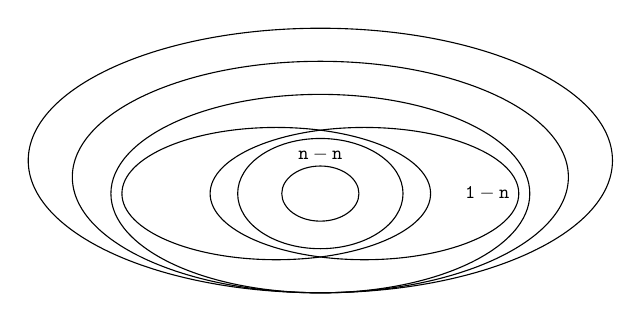
\begin{tikzpicture}[scale=0.7, every node/.style={transform shape}]
   % \draw (0,0) ellipse (5cm and 3cm);
    %\draw (0,0) ellipse (5cm and 3cm);
    %\draw (0,0) ellipse (5cm and 3cm);

\draw(0,0) ellipse (.7cm and .5cm); 
\node (r) at (0,0) {$\rsc$}; 
\draw(0,0) ellipse (1.5cm and 1cm); 
\node (nn) at (0,.7) {$\mathtt{n-n}$}; 

\draw(.8,0) ellipse (2.8cm and 1.2cm); 
\node[left] (n1) at (3.55,0) {$\mathtt{1-n}$}; 
\draw(-.8,0) ellipse (2.8cm and 1.2cm); 
\node[right] (1n) at (-3.5,0) {$\none$}; 

\draw(0,0) ellipse (3.8cm and 1.8cm); 
\node (nn) at (0,1.5) {$\co$}; 

\draw(0,.3) ellipse (4.5cm and 2.1cm); 
\node (nn) at (0,2) {$\oneone$}; 

\draw(0,.6) ellipse (5.3cm and 2.4cm); 
\node (nn) at (0,2.6) {$\asy$}; 

\end{tikzpicture} 

% \begin{tikzpicture}[inclusion/.style={right hook->, thick}]
%     \node (RSC)    at (-1.7,0) {\begin{tabular}{c}synchronous \\ (RSC)\end{tabular}};
%     \node (FIFOnn) at (1,0)  {\begin{tabular}{c}FIFO \\ n-n\end{tabular}}; 
%     \node (FIFO1n) at (3.2,1.5)  {\begin{tabular}{c}FIFO 1-n\end{tabular}};
%     \node (mb)     at (3.2,-1.5) {\begin{tabular}{c}FIFO n-1\\ (mailbox)\end{tabular}};
%     \node (co)     at (5.8,0)  {\begin{tabular}{c}causally\\ ordered\end{tabular}};
%     \node (p2p)    at (8,0) {\begin{tabular}{c}FIFO 1-1\\ (p2p)\end{tabular}};
%     \node (async)  at (10.4,0) {\begin{tabular}{c}asyn-\\ chronous\end{tabular}};
%     \draw[inclusion] (RSC) to (FIFOnn);
%     \draw[inclusion] (FIFOnn.north east) to (FIFO1n.west);
%     \draw[inclusion] (FIFOnn.south east) to (mb.west);
%     \draw[inclusion] (FIFO1n.east) to (co.north west);
%     \draw[inclusion] (mb.east) to (co.south west);
%     \draw[inclusion] (co) to (p2p);
%     \draw[inclusion] (p2p) to (async);
% \end{tikzpicture}
    \caption{\label{fig:hierarchy-of-executions} Hierarchy of communication models based on  sets of
    executions (taken from~\cite{DBLP:journals/fac/ChevrouHQ16})}
\end{figure}

To conclude this brief discussion on queuing networks and executions, we clarify in what sense the operational semantics we introduced in this section are sound and complete with respect to the axiomatic definitions of the communication models we gave in Section~\ref{CH:MSC}. Remember that a linearization $\linrel$ of a MSC
defines a total order on its events, and therefore an execution.

\begin{fact}
A MSC $\msc$ is $\pp$ (resp. $\mb$, $\onensymb$, $\nnsymb$) if and only if there exists
a linearization $\linrel$ of $\msc$ that induces a $\pp$ execution (resp. a $\mb$, $\onensymb$, $\nnsymb$ execution).
\end{fact}

Note that, moreover, a MSC $\msc$ is $\pp$ if and only if \emph{all} of its linearizations induce $\pp$ executions.

\section{MSO definability}\label{sec:MSO}
%\begin{itemize}
%  \item Definition of MSC class for each communication model (alternative definitions)
%  \item MSO-definability of each class
%\end{itemize}

% !TEX root = ../popl-paper.tex

\davidequestion{Don't we need a citation for MSO?}
In Section~\ref{sec:MSC} we introduced seven different communication models and the corresponding classes of MSCs. Here, we show that all of these classes are MSO-definable, i.e. there is a Monadic Second Order Logic formula that defines them. Sometimes it is straightforward, but for some classes of MSCs we have to introduce alternative definitions (equivalent to those given in Section~\ref{sec:MSC}) that are closer to the logic, in order to prove MSO-definability. These alternative definitions will also be heavily used in the following sections for proofs. We first recall the formal definition of MSO logic over MSCs.

\begin{definition}[MSO logic]
The set of MSO formulas over MSCs (over $\Procs$ and $\Msg$) is given by the grammar
$
\phi ::= true \mid x \procrel y \mid x \lhd y \mid \lambda(x) = a \mid x = y \mid x \in X \mid \exists x.\phi \mid \exists X.\phi \mid \phi \vee \phi \mid \neg \phi
$,
where $a \in \Act$, $x$ and $y$ are first-order variables (taken from an infinite set of variables), interpreted as
events of an MSC, and $X$ is a second-order variable, interpreted
as a set of events.
\end{definition}

We use common abbreviations such as $\wedge$, $\Rightarrow$, $\forall$, etc. The satisfaction relation is defined in the standard way and self-explanatory.
For instance, the formula $\neg\exists x.(\bigvee_{a \in \sAct} \lambda(x) = a \;\wedge\; \neg \mathit{matched}(x))$,
with $\mathit{matched}(x) = \exists y.x \lhd y$,
says that there are no unmatched send events. All MSCs of Fig.~\ref{fig:exmscs} satisfy the formula. Given a sentence $\phi$, i.e., a 
formula without free variables,
we let $L(\phi)$ denote the set of MSCs that satisfy $\phi$. Since we have defined the set of MSO formulas over asynchronous 
MSCs, the formula $\asformula = true$ describes the whole set of asynchronous MSCs, i.e. $L(\asformula) = \asMSCs$. It is 
worth mentioning that the (reflexive) transitive closure of a binary relation defined by an MSO formula with free variables 
$x$ and $y$, such as $x \procrel y$, is MSO-definable (more details are given in Appendix~\ref{apx:MSO}). 
The logic can then freely use formulas of the form $x \procrel^+ y$, $x \procrel^* y$ or $x \happensbefore y$.

\paragraph{\bf Peer-to-peer MSCs}
The MSO formula that defines $\ppMSCs$ (i.e. the set of $\pp$-MSCs) directly follows from Definition~\ref{def:pp_msc}:
\[
	\ppformula = \neg \exists s.\exists s'. \left(
	\bigvee_{\substack{p \in \Procs, q \in \Procs}}\;
	\bigvee_{\substack{a,b \in \pqsAct{p}{q}}}\hspace{-1em}
	(\lambda(s) = a \;\wedge\; \lambda(s') = b) \;\wedge\; s \procrel^+ s' \;\wedge\;
	(\psi_1 \vee \psi_2 )
	\right)
\]
where $\psi_1$ and $\psi_2$ are
\[
	\psi_1 = \exists r.\exists r'.\left(
	\begin{array}{ll}
		s \lhd r & \wedge\\
		s' \lhd r' & \wedge\\
		r' \procrel^+ r &
	\end{array}
	\right) \quad \quad
	\psi_2 = (\neg \mathit{matched}(s) \wedge \mathit{matched}(s'))
	\]
	\[
	matched(x) = \exists y. x \lhd y
\]

The property $\ppformula$ says that there cannot be two matched send events $s$ and $s'$, with the same sender and receiver, such that either
\begin{enumerate*}[label={(\roman*)}]
	\item $s \procrel^+ s'$ and their receipts happen in the reverse order, or
	\item $s$ is unmatched and $s'$ is matched.
\end{enumerate*}
% In other words, it ensures that channels operate in FIFO mode, where an unmatched messages blocks the receipt of all the subsequent messages on that channel.
%The set $\ppMSCs$ is therefore MSO-definable as $\ppMSCs=L(\ppformula)$.


\paragraph{\bf Causally ordered MSCs}
As with $\pp$-MSCs, the MSO-definability of $\coMSCs$ follows from Definition~\ref{def:co_msc}, given in Section~\ref{sec:MSC}:
\[
	\coformula = \neg \exists s.\exists s'. \left(
	\bigvee_{\substack{q \in \Procs}}\;
	\bigvee_{\substack{a,b \in \pqsAct{\plh}{q}}}\hspace{-1em}
	(\lambda(s) = a \;\wedge\; \lambda(s') = b) \;\wedge\; s \happensbefore s' \;\wedge\;
	(\psi_1 \vee \psi_2 )
	\right)
\]
where $\psi_1$ and $\psi_2$ have been defined above for the \pp case. The property $\coformula$ says that there cannot be two send events $s$ and $s'$, with the same recipient, such that $s \happensbefore s'$ and either
\begin{enumerate*}[label={(\roman*)}]
	\item their corresponding receive events $r$ and $r'$ happen in the opposite order, i.e. $r' \procrel^+ r$, or
	\item $s$ is unmatched and $s'$ is matched.
\end{enumerate*}
%The set $\coMSCs$ of causally ordered MSCs is therefore MSO-definable as $\coMSCs=L(\coformula)$.


\paragraph{\bf Mailbox MSCs}
For the mailbox communication model, Definition~\ref{def:mb_msc} cannot be easily translated into an MSO formula. Thus, we introduce an alternative definition of $\mb$-MSC that is closer to MSO logic; in particular, we define an additional binary relation that represents a constraint under the $\none$ semantics, which ensures that messages received by a process are sent in the same order as they are received. This definition is shown to be equivalent to Definition~\ref{def:mb_msc} in Appendix~\ref{apx:MSO}.

\begin{definition} [$\none$ alternative]\label{def:n_one_alt}
	For an MSC $\msc = (\Events,\procrel,\lhd,\lambda)$.	Let ${\mbrel} \subseteq \Events \times \Events$
	be defined as $s \mbrel s'$ if there is $q \in \Procs$
	such that $\lambda(s) \in \qsAct{q}$,
	$\lambda(s') \in \qsAct{q}$, and either:
	\begin{itemize}%\itemsep=0.5ex
		\item $s \in \Matched{\msc}$ and $s' \in \Unm{\msc}$, or
		\item $s \lhd f_1$ and $s' \lhd f_2$ for some $f_1,f_2 \in \Events_q$ such that $f_1 \procrel^+ f_2$.
	\end{itemize}

	We let ${\mbpartial} = ({\procrel} \,\cup\, {\lhd} \,\cup\, {\mbrel})^\ast$.
	$\msc $ is a \emph{$\none$-MSC}
	if ${\mbpartial}$ is a partial order.
\end{definition}
The ${\mbrel}$ relation ensures that send events addressed to the same process are executed in an order that is suitable for the $\none$ communication model. If ${\mbpartial}$ is a partial order, it means that it is possible to find a linearization $\linrel$, such that $\linrel \;\subseteq\; \mbpartial$. It is easy to see that such a linearization is exactly what we called a $\none$-linearization in Definition~\ref{def:mb_msc}.
%Finally notice  that ${\le} \subseteq {\mbpartial}$. Hence entailing that a \mb-MSC is also a \pp-MSC.
The MSO-definability of $\mbMSCs$ follows from Definition~\ref{def:n_one_alt}; in particular, note that 
$\mbpartial$ is reflexive and transitive by definition, 
thus we just have to check antisymmetry:
\[
	\mbformula = \ppformula \;\wedge\; \neg \exists x.\exists y.(\neg (x = y) \wedge x \mbpartial y \wedge y \mbpartial x)
\]
%This formula closely follows Definition~\ref{def:n_one_alt}. The set $\mbMSCs$ of $\none$ MSCs is therefore MSO-definable as $\mbMSCs=L(\mbformula)$.

where $x \mbpartial y$ is obtained as the MSO-definable reflexive transitive closure of
the union of the MSO-definable relations $\procrel$, $\lhd$, and $\mbrel$; 
we may define $x \mbrel y$ as:
\[
x \mbrel y =
\displaystyle
\hspace{-1em}\bigvee_{\substack{q \in \Procs\\a,b \in \qsAct{q}}}\hspace{-1em}
(\lambda(x) = a \;\wedge\; \lambda(y) = b)
\wedge
\left(
\begin{array}{rl}
& \mathit{matched}(x) \wedge \neg \mathit{matched}(y)\\[1ex]
\vee & \exists x'.\exists y'. (x \lhd x' \;\wedge\; y \lhd y' \;\wedge\; x' \procrel^+ y')
\end{array}
\right).
\]



\paragraph{\bf \onen MSCs}

As with the mailbox communication model, we give an alternative definition of $\onen$ MSC; the equivalence with Definition~\ref{def:one_n} is shown in Appendix~\ref{apx:MSO}.

\begin{definition} [$\onen$ alternative]\label{def:one_n_alt}
	For an MSC $\msc = (\Events,\procrel,\lhd,\lambda)$, let ${\onenrel} \subseteq \Events \times \Events$ be defined as $e_1 \onenrel e_2$ if there are two events $e_1$ and $e_2$, and $p \in \Procs$ such that either:
	\begin{itemize}%\itemsep=0.5ex
		\item $\lambda(e_1) \in \psAct{p}$, $\lambda(e_2) \in \psAct{p}$, $e_1 \in \Matched{\msc}$, and $e_2 \in \Unm{\msc}$, or
		\item $\lambda(e_1) \in \prAct{p}$, $\lambda(e_2) \in \prAct{p}$, $s_1 \lhd e_1$ and $s_2 \lhd e_2$ for some $s_1,s_2 \in \Events_p$, and $s_1 \procrel^+ s_2$.
	\end{itemize}

	We let ${\onenpartial} = ({\procrel} \,\cup\, {\lhd} \,\cup\, {\onenrel})^\ast$.
		%\begin{definition}\label{def:mailbox-msc}
	$\msc$ is a \emph{$\onen$ MSC}
	if ${\onenpartial}$ is a partial order.
\end{definition}

The ${\onenrel}$ relation ensures that messages sent by a process are sent and received in an order that is suitable for the $\onen$ communication. Since ${\onenpartial}$ is a partial order, it is possible to find a linearization $\linrel$ such that $\linrel \;\subseteq\; \onenpartial$. It is not difficult to see that such a linearization is exactly what we called a $\onen$ linearization in Definition~\ref{def:one_n}.
The MSO formula that defines $\onenMSCs$ follows from  Definition~\ref{def:one_n_alt}:
\[
	\onenformula = \neg \exists x.\exists y.(\neg (x = y) \wedge x \onenpartial y \wedge y \onenpartial x)
\]
Recall that $\onenpartial$ is the union of the MSO-definable relations $\procrel$, $\lhd$, and $\onenrel$. In particular, we can define $x \onenrel y$ as
\[
x \onenrel y =
\begin{array}{rl}
& \left(
	\bigvee_{\substack{p \in \Procs\\a,b \in \psAct{p}}}\hspace{-1em}
	(\lambda(x) = a \;\wedge\; \lambda(y) = b)
	\;\wedge\; \mathit{matched}(x) \;\wedge\; \neg \mathit{matched}(y)
\right) \;\vee\\
& \left(
	\bigvee_{\substack{p \in \Procs\\a,b \in \prAct{p}}}\hspace{-1em}
	(\lambda(x) = a \;\wedge\; \lambda(y) = b)
	\;\wedge\;
	\exists x'.\exists y'. (x' \lhd x \;\wedge\; y' \lhd y \;\wedge\; x' \procrel^+ y')
\right)\\
\end{array}
\]
%The MSO formula for $x \onenrel y$ closely follows Definition~\ref{def:one_n_alt}. The set $\onenMSCs$ of $\onen$ MSCs is therefore MSO-definable as $\onenMSCs=L(\onenformula)$.

%Finally it is worth noting that ${\le} \subseteq {\onenpartial}$.
%\cinzia{maybe move previous sentence to next section}

\paragraph{\bf \nn MSCs}

In order to show the MSO-definability of \nn MSCs we give an alternative definition and prove that it is equivalent to Definition~\ref{def:n_n}. Unlike mailbox and $\onen$ communication models, the equivalence is not trivial.

\begin{definition} [$\nn$ alternative]\label{def:n_n_alt}
	For an MSC $\msc = (\Events,\procrel,\lhd,\lambda)$, let ${\nnrel} = ({\procrel} \,\cup\, {\lhd} \,\cup\, {\mbrel} \,\cup\, {\onenrel})^\ast$. We define  $\nnbowtie \subseteq \Events \times \Events$,  such that $e_1 \nnbowtie e_2$ if one of the following holds:
	\begin{enumerate}%\itemsep=0.5ex
		\item $e_1 \nnrel e_2$
		\item $\lambda(e_1) \in \prAct{\plh}$, $\lambda(e_2) \in \prAct{\plh}$, $s_1 \lhd e_1$ and $s_2 \lhd e_2$ for some $s_1,s_2 \in \Events$, $s_1 \nnrel s_2$ and $e_1 \notnnrel e_2$.
		\item $\lambda(e_1) \in \psAct{\plh}$, $\lambda(e_2) \in \psAct{\plh}$, $e_1 \lhd r_1$ and $e_2 \lhd r_2$ for some $r_1,r_2 \in \Events$, $r_1 \nnrel r_2$ and $e_1 \notnnrel e_2$.
		\item $e_1 \in \Matched{\msc}$, $e_2 \in \Unm{\msc}$, $e_1 \notnnrel e_2$.
	\end{enumerate}

	%Note that $\mbpartial \subseteq \nnrel$, $\onenpartial \subseteq \nnrel$, and $\nnrel \subseteq\; \nnbowtie$.
	$\msc $ is a \emph{$\nn$ MSC}
	if ${\nnbowtie}$ is acyclic.
\end{definition}

To prove that Definition~\ref{def:n_n} and Definition~\ref{def:n_n_alt} are equivalent, we need some preliminary results and definitions. Please note that missing proofs can be found in Appendix~\ref{apx:MSO}.

\begin{restatable}{proposition}{nnfirstprop}
\label{prop:nn_first_prop}
	Let $\msc$ be an MSC. Given two matched send events $s_1$ and $s_2$, and their respective receive events $r_1$ and $r_2$, $r_1 \nnbowtie r_2 \implies s_1 \nnbowtie s_2$.
\end{restatable}

\begin{restatable}{proposition}{nnsecondprop}
\label{prop:n_n_cycl}
	Let $\msc$ be an MSC. If $\nnbowtie$ is cyclic, then $\msc$ is not $\nn$.
\end{restatable}

Let the \emph{Event Dependency Graph} (EDG) of a $\nn$ MSC $\msc$ be a graph that has events as nodes and an edge between two events $e_1$ and $e_2$ if $e_1 \nnbowtie e_2$. We now present an algorithm that, given the EDG of an $\nn$ MSC $\msc$, computes a $\nn$ linearization of $\msc$. We then show that, if $\nnbowtie$ is acyclic, this algorithm always terminates correctly. This, along with Proposition~\ref{prop:n_n_cycl}, effectively shows that Definition~\ref{def:n_n} and Definition~\ref{def:n_n_alt} are equivalent.

\paragraph*{Algorithm for finding a $\nn$ linearization}
The input of this algorithm is the EDG of an MSC $\msc$, and it outputs a valid $\nn$ linearization for $\msc$, if $\msc$ is $\nn$. The algorithm works as follows:
\begin{enumerate}
	\item If there is a matched send event $s$ with in-degree 0 in the EDG, add $s$ to the linearization and remove it from the EDG, along with its outgoing edges, then jump to step 5. Otherwise, proceed to step 2.
	\item If there are no matched send events in the EDG and there is an unmatched send event $s$ with in-degree 0 in the EDG, add $s$ to the linearization and remove it from the EDG, along with its outgoing edges, then jump to step 5. Otherwise, proceed to step 3.
		\item If there is a receive event $r$ with in-degree 0 in the EDG, such that $r$ is the receive event of the first message whose sent event was already added to the linearization, add $r$ to the linearization and remove it from the EDG, along with its outgoing edges, then jump to step 5. Otherwise, proceed to step 4.
		\item Throw an error and terminate.
		\item If all the events of $\msc$ were added to the linearization, return the linearization and terminate. Otherwise, go back to step 1.
\end{enumerate} 

We now need to show that 
\begin{enumerate*}[label={(\roman*)}]
	\item if this algorithm terminates correctly (i.e. step 4 is never executed), it returns a $\nn$ linearization, and 
	\item if $\nnbowtie$ is acyclic, the algorithm always terminates correctly.
\end{enumerate*}

\begin{proposition}
	If the above algorithm returns a linearization for an MSC $\msc$, it is a $\nn$ linearization.
\end{proposition}
\begin{proof}
	Step 2 ensures that the order (in the linearization) in which matched messages are sent is the same as the order in which they are received. Moreover, according to step 3, an unmatched send events is added to the linearization only if all the matched send events were already added.
\end{proof}

\begin{example}
	Fig.~\ref{fig:nn_algo_ex} shows an example of $\nnsymb$-MSC and its EDG. We use it to show how the algorithm that builds a $\nnsymb$-linearization works. Note that, for convenience, not all the edges of the EDG have been drawn, but those missing would only connect events for which there is already a path is our drawing; these edges do not have any impact on the execution of the algorithm. We start by applying step 1 on the event $!5$, which has in-degree 0. The algorithm starts to build a linearization using $!5$ as the first event, and all the outgoing edges of $!5$ are removed from the EDG, along with the event itself. Now, $!1$ has in-degree 0 and we can apply again step 1. The partial linearization becomes $!5\;!1$. Similarly, we can then apply step 1 on $!2$ and $!3$ to get the partial linearization $!5\;!1\;!2\;!3$. At this point, step 1 and 2 cannot be applied, but we can use step 3 on $?5$, which gets added to linearization. We then apply step 3 also to $?1$ and $?2$, followed by step 1 on $!4$, step 2 on $!6$ (which is an unmatched send event), and step 3 on $?3$ and $?4$. Finally, all the events of the MSC have been added to our linearization, which is $!5\;!1\;!2\;!3\;?5\;?1\;?2\;!4\;!6\;?3\;?4$. Note that this is a $\nnsymb$-linearization.
\end{example}

\begin{figure}[t] 
\begin{subfigure}[c]{0.4\textwidth}\raggedleft
\begin{tikzpicture}[ scale = .7,every node/.style={transform shape}]
\newproc{0}{p}{-3.3}; 
\newproc{1.2}{q}{-3.3}; 
\newproc{2.4}{r}{-3.3}; 
\newproc{3.6}{s}{-3.3}; 
\newproc{4.8}{t}{-3.3};

\newmsgm{0}{2.4}{-0.6}{-2.4}{5}{0.8}{black};
\newmsgm{0}{1.2}{-1}{-1}{1}{0.65}{black};
\newmsgm{2.4}{1.2}{-1.4}{-1.4}{2}{0.5}{black};
\newmsgm{2.4}{3.6}{-1.8}{-1.8}{3}{0.5}{black};
\newmsgm{1.2}{3.6}{-2.8}{-2.8}{4}{0.2}{black};
\newmsgum{3.6}{4.8}{-1}{6}{0.5}{black}; 

\end{tikzpicture} 
\end{subfigure} 
\hfill
\begin{subfigure}[c]{0.4\textwidth}\raggedright
	\begin{tikzpicture}[scale = .6,every node/.style={transform shape}] 
\begin{scope} 
\node (r4) at (0,0) {$?4$};
     \node (s4) at (-1,-1) {$!4$};
     \node (r3) at (1,-1) {$?3$};
     \node (r2) at (-1,-2) {$?2$};
     \node (s3) at (1,-3) {$!3$};
     \node (s6) at (2,-2) {$!6$};
     \node (r1) at (-1,-3) {$?1$};
     \node (s1) at (-1,-4) {$!1$};
     \node (r5) at (-2,-4) {$?5$};
     \node (s5) at (-1,-5) {$!5$};
     \node (s2) at (-2,-6) {$!2$};	

     \draw[->] (s2) -- (r5); 
     \draw[->] (s5) -- (r5);
     \draw[->] (s5) -- (s1);
     \draw[->] (s1) -- (r1); 
     \draw[->, color = blue] (r5) -- (r1);
     \draw[->] (r1) -- (r2);
     \draw[->] (r2) -- (s4);
     \draw[->] (s4) -- (r4);
     \draw[->, color = Green, dashed] (s3) -- (s6);
     \draw[->] (s3) -- (r3);
     \draw[->] (s6) -- (r3); 
     \draw[->, color = red] (r3) -- (r4);
     \draw[->, color = blue ] (r2) -- (r3); 
 
     \draw[->] (s2) to[bend left= 40] (r2);  
     \draw[->] (s2) to[bend right= 70] (s3);
     \draw[->, color = Green, dashed] (s2) to[bend right= 70] (s6);
     \draw[->, color = red] (s1) to[bend left= 60] (s2); 
     \draw[->, color = Green, dashed] (s1) to[bend right= 40] (s6); 
     \draw[->, color = Green, dashed] (s4) to[bend right= 30] (s6); 
\end{scope} 
     \begin{scope}[shift = {(2.5,-4.5)}]
 	     \draw[->] (0,0) -- (.8,0); 
 	     \draw[->, color = blue] (0,-.5) -- (.8,-.5); 
 	     \draw[->, color = red] (0,-1) -- (.8,-1); 
 	     \draw[->, color = Green, dashed] (0,-1.5) -- (.8,-1.5); 
	\node[right] (1) at (.8,0)  {$= (\procrel / \lhd)$}; 
	\node[right] (2) at (.8,-.5) {$= (\onenrel)$}; 
	\node[right] (3) at (.8, -1) {$= (\mbrel)$}; 
	\node[right] (4) at (.8,-1.5) {$=$ (other edges)};
     \end{scope} 
\end{tikzpicture}
\end{subfigure}
    \caption{An MSC and its EDG. In the EDG, only meaningful edges are shown.}
    \label{fig:nn_algo_ex}
\end{figure} 


The proof for the next proposition is quite intricate, and it can be found in Appendix~\ref{apx:MSO}.

\begin{restatable}{proposition}{nnalgotermination}
\label{prop:nn_algo_term}
	Given an MSC $\msc$, the above algorithm always terminates correctly if $\nnbowtie$ is acyclic.
\end{restatable}

Proposition~\ref{prop:n_n_cycl} and Proposition~\ref{prop:nn_algo_term} are sufficient to prove that Definition~\ref{def:n_n_alt} and Definition~\ref{def:n_n} are equivalent.
Based on Definition~\ref{def:n_n_alt}, we can finally write an MSO formula for $\nn$ MSCs:
\[
	\nnformula = \neg \exists x.\exists y.(\neg (x = y) \wedge x \nnbowtie y \wedge y \nnbowtie x)
\]
where we can define $x \nnbowtie y$ as
\[
	x \nnbowtie y =
	\begin{array}{rl}
	& \left(
		\bigvee_{\substack{a,b \in \psAct{\plh}}}
		(\lambda(x) = a \;\wedge\; \lambda(y) = b)
		\;\wedge\; \mathit{matched}(x) \;\wedge\; \neg \mathit{matched}(y)
	\right) \;\vee\\
	& (x \nnrel y) \quad \vee \quad \psi_3 \quad \vee \quad \psi_4\\
	\end{array}
\]

\noindent where $\psi_3$ and $\psi_4$ are defined as
\[
	\psi_3 =
	\begin{array}{rl}
		& \bigvee_{\substack{a,b \in \prAct{\plh}}}
		  (\lambda(x) = a \;\wedge\; \lambda(y) = b)
		  \;\wedge\; \\
		& \exists x'.\exists y'.(x' \lhd x \;\wedge\; y' \lhd y) \;\wedge\; (x' \nnrel y') \;\wedge\; \neg(x \nnrel y)\\
	\end{array}
\]
\[
	\psi_4 =
	\begin{array}{rl}
		& \bigvee_{\substack{a,b \in \psAct{\plh}}}
		  (\lambda(x) = a \;\wedge\; \lambda(y) = b)
		  \;\wedge\; \\
		& \exists x'.\exists y'.(x \lhd x' \;\wedge\; y \lhd y') \;\wedge\; (x' \nnrel y') \;\wedge\; \neg(x \nnrel y)\\
	\end{array}
\]

Note that $\nnrel$ is MSO-definable, since it is defined as the reflexive transitive closure of MSO-definable relations.

\paragraph{\bf Realizable with Synchronous Communication MSCs} 

Following the characterization given in \cite[Theorem 4.4]{DBLP:journals/dc/Charron-BostMT96}, we also give an alternative definition of $\rsc$-MSC (the equivalence with Definition~\ref{def:rsc} is shown in Appendix~\ref{apx:MSO}). We first need to introduce the concept of \emph{crown}.

\begin{definition} [crown]
	Let $\msc$ be an MSC. A \emph{crown} of size $k$ in $\msc$ is a sequence $\langle(s_i,r_i),\, i \in \{1,\dots,k\}\rangle$ of pairs of corresponding send and receive events such that
	\[
		s_1 \happensbeforestrict r_2, s_2 \happensbeforestrict r_3, \dots, s_{k-1} \happensbeforestrict r_k, s_k \happensbeforestrict r_1.
	\]
\end{definition}
\davide{Should I specify somewhere that $\happensbeforestrict = (\procrel \cup \lhd)^+$ or is it clear?}

\begin{definition} [$\rsc$ alternative]\label{def:rsc_alt}
	An MSC $\msc = (\Events,\procrel,\lhd,\lambda)$ is a \emph{RSC MSC} if and only if it does not contain any crown.
\end{definition}

%Such a linearization will be referred to as a \emph{$\rsc$ linearization}.

The following MSO formula derives directly from previous  definition:
\[\Phi_{\rsc} = \neg \exists s_1.\exists s_2. s_1 \varpropto s_2 \;\wedge\; s_2 \varpropto^\ast s_1
\]
\noindent where $\varpropto$ is defined as
\[
s_1 \varpropto s_2 =
\bigvee_{\substack{e \in \sAct}}(\lambda(s_1) = e) \;\wedge\;
s_1 \neq s_2 \;\wedge\;
\exists r_2. (s_1 < r_2 \;\wedge\; s_2 \lhd r_2)
\]


% THIS IS WRONG!
% We show that the opposite direction is also true, which implies that the class of $\nn$ MSCs is equivalent to the class of $onen$ MSCs. The following example gives an intuition of the formal proof, which will be given right after.

% \begin{proposition}
% 	Every $\onen$ MSC without unmatched messages is an $\nn$ MSC.
% \end{proposition}
% \begin{proof}
% Let $\msc$ be a $\onen$ MSC without unmatched messages, and let $L$ be a $\onen$ linearization. We will show that, by reordering some of the events in $L$, we are always able to obtain a $\nn$ linearization for $\msc$. The algorithm works as follow:
% \begin{enumerate}
% 	\item Find a pair $(m_1,m_2)$ of distinct messages such that their send order in $L$ is the inverse of the receive order\footnote{Note that $L$ is already a $\nn$ linearization if such a pair does not exist}. This can only happen if there is not a causal path between $s_1$ and $s_2$, i.e $s_1 \le \ge s_2$, where $s_i$ is the send event of message $m_i$. To see why, suppose w.l.o.g. that $s_1 \le s_2$. As seen in the proof of Proposition~\ref{prop:onen_mb_no_unmatched}, there must be a message $m_k$ sent by the same process that sent $s_1$, such that we have $r_1 \onenrel r_k \le r_2$, and in particular $r_1 \onenpartial r_2$. Therefore, if $s_1 \le s_2$, the receive order has to match the send order in $L$ and it will never be the opposite.
% 	\item Suppose, w.l.o.g. that $s_2 \linrel s_1$ and $r_1 \linrel r_2$, and we saw that $s_1 \le \ge s_2$. We would like to invert the order of $s_1$ and $s_2$ in the linearization, so that it matches the receive order. If we simply swap $s_2$ and $s_1$ in $L$, the new linearization could be invalid for $\msc$; for instance, there might be some events between $s_2$ and $s_1$ (in the linearization $L$) that need to happen before $s_1$. However, we show that it is still possible to invert the order of $s_1$ and $s_2$ without invalidating the linearization. Suppose that $s_2$ and $s_1$ are the $i$-th and the $j$-th events of $L$, respectively, where $i<j$. The idea is to move $s_2$ right before $s_1$, along with all the events on which $s_1$ depends, that are between $s_2$ and $s_1$ in $L$; we say that $s_1$ depends on an event $e$ if $e \onenpartial s_1$.
% \end{enumerate}
% \end{proof}





% \davidequestion{The following formula should be wrong... I cannot use $n$ in an MSO formula}
% \[
% 	\rscformula =
% 	\begin{array}{rl}
% 		& \forall x.\left(\bigvee_{a \in \psAct{\plh}} \lambda(x) = a \;\implies\; \mathit{matched}(x)\right) \;\wedge\; \\
% 		& \neg \left(
% 			\bigvee_{k=1}^n \left(
% 			\exists s_1 \cdots s_k. \exists r_1 \cdots r_k.
% 			\bigwedge_{i=1}^k (s_i \lhd r_i \;\wedge\; s_i \le r_{(i+1)\%k})
% 		\right)
% 		\right)\\
% 	\end{array}
% \]
% where $n$ is the total number of messages. The formula checks that there are no unmatched send events and that in the conflict graph there is no cycle, of any length, whose edges are all SR.



%
%\section{Equivalence of the two definitions}
%\begin{itemize}
%  \item TODO...
%\end{itemize}

\section{Hierarchy of classes of MSCs} \label{sec:hierarchy}

% \section{(7) Hierarchy of classes of MSCs}

As mentioned in Section~\ref{sec:com_models_overview}, the classes of MSCs for all the 7 communication models that we presented form a clear hierarchy, which is shown in Fig.~\ref{fig:msc_hierarchy_full}. In this section we will provide proofs to support this claim. For the simplest cases, we just give intuitive explanations; please refer to Appendix~\ref{apx:hierarchy} for the formal proofs.

\medskip

First of all, note that every $\oneone$ MSC is an asynchronous MSC by definition. Moreover, Fig.~\ref{fig:fully_asy_ex} shows an example of MSC that is asynchronous but not $\oneone$, hence we have $\ppMSCs \subset \asMSCs$. 
In the causally ordered communication model, any two messages addressed to the same process are received in an order that matches the causal order in which they are sent. In particular, it is easy to see that each causally ordered MSC is also a $\oneone$ MSC, since for any two messages sent by a process $p$ to another process $q$, the two send events are causally ordered. The MSC shown in Fig.~\ref{fig:pp_ex} is $\oneone$, but not $\co$, hence we can conclude that $\coMSCs \subset \ppMSCs$.
We now show that each $\none$ MSC is a causally ordered MSC.

\begin{proposition} \label{prop:mb_is_co}
	Every $\none$ MSC is a causally ordered MSC.
\end{proposition}
\begin{proof}
Let $\msc$ be a $\none$ MSC and $\linrel$ a $\none$ linearization of it. Recall that a linearization has to respect the happens-before partial order over $\msc$, i.e. $\happensbefore\,\subseteq\, \linrel$. Consider any two send events $s$ and $s'$, such that $\lambda(s)=\pqsAct{\plh}{q}$, $\lambda(s')=\pqsAct{\plh}{q}$ and $s \happensbefore s'$. Since $\happensbefore\,\subseteq\, \linrel$, we have that $s \linrel s'$ and, by the definition of $\none$ linearization, either
\begin{enumerate*}[label={(\roman*)}]
	\item $s' \in \Unm{\msc}$, or 
	\item $s,s' \in \Matched{\msc}$, $s \lhd r$, $s' \lhd r'$ and $r \linrel r'$. 
\end{enumerate*}
The former clearly respects the definition of causally ordered MSC, so let us focus on the latter. Note that $r$ and $r'$ are two receive events executed by the same process, hence $r \linrel r'$ implies $r \procrel^+ r'$. It follows that $\msc$ is a causally ordered MSC.
\end{proof}

Fig.~\ref{fig:co_no_none} shows an example of causally ordered MSC that is not $\none$. It is causally ordered because we cannot even find two messages, addressed to the same process, such that the corresponding send events are causally related; on the contrary, the MSC is not $\none$ because we have $!4 \mbrel !1$ and $!2 \mbrel !3$, which lead to a cyclic dependency, e.g. $!1 \procrel !2 \mbrel !3 \procrel !4 \mbrel !1$. This example and Proposition~\ref{prop:mb_is_co} prove that $\mbMSCs \subset \coMSCs$.

\begin{figure}[t]
	\captionsetup[subfigure]{justification=centering}
\begin{subfigure}[t]{0.2\textwidth}\centering
	\begin{tikzpicture}[scale=0.7, every node/.style={transform shape}]
		\newproc{0}{p}{-2.2};
		\newproc{1}{q}{-2.2};
		\newproc{2}{r}{-2.2};
		\newproc{3}{s}{-2.2};
		
		\newmsgm{0}{3}{-0.3}{-2.0}{1}{0.1}{black};
		\newmsgm{0}{1}{-1.0}{-1.0}{2}{0.3}{black};
		\newmsgm{2}{1}{-1.2}{-1.2}{3}{0.3}{black};
		\newmsgm{2}{3}{-1.6}{-1.6}{4}{0.5}{black};
		
	\end{tikzpicture}
	\caption{$\co$, not $\none$.}
	\label{fig:co_no_none}
\end{subfigure}
\begin{subfigure}[t]{0.25\textwidth}\centering
	\begin{tikzpicture}[scale=0.7, every node/.style={transform shape}]
		\newproc{0}{p}{-2.2};
		\newproc{1}{q}{-2.2};
		\newproc{2}{r}{-2.2};
		
		\newmsgum{0}{1}{-0.8}{1}{0.3}{black};
		\newmsgm{0}{2}{-1.5}{-1.5}{2}{0.15}{black};
		
	\end{tikzpicture}
	\caption{$\none$, not $\onen$ MSC.}
	\label{fig:mb_no_onen}
\end{subfigure}
% \hfill
\begin{subfigure}[t]{0.2\textwidth}\centering
	\begin{tikzpicture}[scale=0.7, every node/.style={transform shape}]
		\newproc{0}{p}{-2.2};
		\newproc{1}{q}{-2.2};
		\newproc{2}{r}{-2.2};
		\newproc{3}{s}{-2.2};
	
		\newmsgm{3}{2}{-0.1}{-1.9}{1}{0.2}{black};
		\newmsgm{0}{3}{-0.7}{-0.7}{2}{0.1}{black};
		\newmsgm{0}{1}{-1.3}{-1.3}{3}{0.3}{black};
		\newmsgm{1}{2}{-1.6}{-1.6}{4}{0.3}{black};
			
	\end{tikzpicture}
	\caption{$\onen$ MSC, not $\nn$.}
	\label{fig:onen_no_nn}
\end{subfigure}
\begin{subfigure}[t]{0.2\textwidth}\centering
	\begin{tikzpicture}[scale=0.7, every node/.style={transform shape}]
		\newproc{0}{p}{-2.2};
		\newproc{2}{q}{-2.2};	
	
		\newmsgm{0}{2}{-0.5}{-1.7}{1}{0.1}{black};
		\newmsgm{2}{0}{-0.5}{-1.7}{2}{0.1}{black};
			
	\end{tikzpicture}
	\caption{$\nn$, not $\rsc$.}
	\label{fig:nn_no_rsc}
\end{subfigure}
\caption{Examples of MSCs for various communication models.}\label{fig:exmscs_2}
\end{figure}

The relation between $\onen$ and $\none$ MSCs is not as straghtforward as those seen so far. For convenience, we will start by only considering MSCs without unmatched messages. 

\begin{proposition} \label{prop:onen_mb_no_unmatched}
	Every $\onen$ MSC without unmatched messages is a $\none$ MSC.
\end{proposition}
\begin{proof}
We show that the contrapositive is true, i.e. if an MSC is not mailbox (and it does not have unmatched messages), it is also not $\onen$. Suppose $\msc$ is an asynchronous MSC, but not mailbox. There must be a cycle $\xi$ such that  $e \mbpartial e$, for some event $e$. Recall that ${\mbpartial} = ({\procrel} \,\cup\, {\lhd} \,\cup\, {\mbrel})^\ast$ and ${\le} = ({\procrel} \cup {\lhd})^\ast$. We can always explicitely write a cycle $e \mbpartial e$ only using $\mbrel$ and $\le$. For instance, there might be a cycle $e \mbpartial e$ because we have that $e \mbrel f \happensbefore g \mbrel h \mbrel i \happensbefore e$. Consider any two adiacent events $s_1$ and $s_2$ in the cycle $\xi$, where $\xi$ has been written using only $\mbrel$ and $\le$, and we never have two consecutive $\le$\footnote{This is always possible, since $a \happensbefore b \happensbefore c$ is written as $a \happensbefore c$.}. We have two cases:
\begin{enumerate}
	\item $s_1 \mbrel s_2$. We know, by definition of $\mbrel$, that $s_1$ and $s_2$ must be two send events and that $r_1 \procrel^+ r_2$, where $r_1$ and $r_2$ are the receive events that match with $s_1$ and $s_2$, respectively (we are not considering unmatched messages by hypothesis).
	\item $s_1 \happensbefore s_2$. Since $\msc$ is asynchronous by hyphotesis, $\xi$ has to contain at least one $\mbrel$\footnote{If that was not the case, $\le$ would also be cyclic and $\msc$ would not be an asynchronous MSC.}; recall that we also wrote $\xi$ in such a way that we do not have two consecutive $\le$. It is not difficult to see that $s_1$ and $s_2$ have to be send events, since they belong to $\xi$. We have two cases:
	\begin{enumerate}
		\item $r_1$ is in the causal path, i.e. $s_1 \lhd r_1 \happensbefore s_2$. In particular, note that $r_1 \happensbefore r_2$.
		\item $r_1$ is not in the causal path, hence there must be a message $m_k$ sent by the same process that sent $s_1$, such that $s_1 \procrel^+ s_k \lhd r_k \happensbefore s_2 \lhd r_2$, where $s_k$ and $r_k$ are the send and receive events associated with $m_k$, respectively. Since messages $m_1$ and $m_k$ are sent by the same process and $s_1 \procrel^+ s_k$, we should have $r_1 \onenrel r_k$, according to the $\onen$ semantics. In particular, note the we have $r_1 \onenrel r_k \happensbefore r_2$.
	\end{enumerate}
	In both case (a) and (b), we conclude that $r_1 \onenpartial r_2$. Recall that ${\onenpartial} = ({\procrel} \,\cup\, {\lhd} \,\cup\, {\onenrel})^\ast$.
\end{enumerate}
Notice that, for either cases, a relation between two send events $s_1$ and $s_2$ (i.e. $s_1 \mbrel s_2$ or $s_1 \happensbefore s_2$) always implies a relation between the respective receive events $r_1$ and $r_2$, according to the $\onen$ semantics. It follows that $\xi$, which is a cycle for the $\mbpartial$ relation, always implies a cycle for the $\onenpartial$ relation\footnote{If $\onenpartial$ is cyclic, $\msc$ is not a $\onen$ MSC.}, as shown by the following example. Let $\msc$ be a non-mailbox MSC, and suppose we have a cycle $s_1 \mbrel s_2 \mbrel s_3 \happensbefore s_4 \mbrel s_5 \happensbefore s_1$. $s_1 \mbrel s_2$ falls into case (1), so it implies $r_1 \procrel^+ r_2$. The same goes for $s_2 \mbrel r_3$, which implies $r_2 \procrel^+ r_3$. $s_3 \happensbefore s_4$ falls into case (2), and implies that $r_3 \onenpartial r_4$. $s_4 \mbrel s_5$ falls into case (1) and it implies $r_4 \procrel^+ r_5$. $s_5 \happensbefore s_1$ falls into case (2) and implies that $r_5 \onenpartial r_1$. Putting all these implications together, we have that $r_1 \procrel^+ r_2 \procrel^+ r_3 \onenpartial r_4 \procrel^+ r_5 \onenpartial r_1$, which is a cycle for $\onenpartial$. Note that, given any cycle for $\mbpartial$, we are always able to apply this technique to obtain a cycle for $\onenpartial$.
\end{proof}

The opposite direction is also true and the proof, which can be found in the Appendix~\ref{apx:hierarchy}, uses the same technique to prove that a cycle for $\onenpartial$ always implies a cycle for $\mbpartial$.

\begin{restatable}{proposition}{mbonennounmatched} 
\label{prop:mb_onen_no_unmatched}
	Every $\none$ MSC without unmatched messages is a $\onen$ MSC.
\end{restatable}

Interestingly enough, Proposition~\ref{prop:onen_mb_no_unmatched} and \ref{prop:mb_onen_no_unmatched} show that the classes of $\none$ and $\onen$ MSCs are effectively equivalent if we do not allow unmatched messages. As we will prove, this will change when we add unmatched messages into the mix. However, Proposition~\ref{prop:onen_mb_no_unmatched} still holds.

\begin{proposition} \label{prop:onen_mb_unmatched}
	Every $\onen$ MSC is a $\none$ MSC, i.e. $\onenMSCs \subseteq \mbMSCs$.
\end{proposition}
\begin{proof}
Let $\msc$ be an asynchronous MSC. The proof proceeds in the same way as the one of Proposition~\ref{prop:onen_mb_no_unmatched}, but unmatched messages introduce some additional cases. Consider any two adiacent events $s_1$ and $s_2$ in a cycle $\xi$ for $\mbpartial$, where $\xi$ has been written using only $\mbrel$ and $\le$, and we never have two consecutive $\le$. These are some additional cases:
\begin{enumerate}\setcounter{enumi}{2}
	\item $u_1 \mbrel s_2$, where $u_1$ is the send event of an unmatched message. This case never happens because of how $\mbrel$ is defined.
	\item $u_1 \happensbefore u_2$, where $u_1$ and $u_2$ are both send events of unmatched messages. Since both $u_1$ and $u_2$ are part of the cycle $\xi$, there must be an event $s_3$ such that $u_1 \happensbefore u_2 \mbrel s_3$. However, $u_2 \mbrel s_3$ falls into case (3), which can never happen.
	\item $u_1 \happensbefore s_2$, where $u_1$ is the send event of an unmatched message and $s_2$ is the send event of a matched message. Since we have a causal path between $u_1$ and $s_2$, there has to be a message $m_k$, sent by the same process that sent $m_1$, such that $u_1 \procrel^+ s_k \lhd r_k \happensbefore s_2 \lhd r_2$\footnote{Note that we can have $m_k = m_2$}, where $s_k$ and $r_k$ are the send and receive events associated with $m_k$, respectively. Since messages $m_1$ and $m_k$ are sent by the same process and $m_1$ is unmatched, we should have $s_k \onenrel u_1$, according to the $\onen$ semantics, but $u_1 \procrel^+ s_k$. It follows that if $\xi$ contains $u_1 \happensbefore s_2$, we can immediately conclude that $\msc$ is not a $\onen$ MSC.
	\item $s_1 \mbrel u_2$,  where $s_1$ is the send event of a matched message and $u_2$ is the send event of an unmatched message. Since both $s_1$ and $u_2$ are part of a cycle, there must be an event $s_3$ such that $s_1 \mbrel u_2 \happensbefore s_3$; we cannot have $u_2 \mbrel s_3$, because of case (3). $u_2 \happensbefore s_3$ falls into case (5), so we can conclude that $\msc$ is not a $\onen$ MSC.
\end{enumerate}
We showed that cases (3) and (4) can never happen, whereas cases (5) and (6) both imply that $\msc$ is not $\onen$. If we combine them with the cases described in Proposition~\ref{prop:onen_mb_no_unmatched} we have the full proof.
\end{proof}

The MSC in Fig.~\ref{fig:mb_no_onen} shows a simple example of an MSC with unmatched messages that is $\none$ but not $\onen$. This, along with Proposition~\ref{prop:onen_mb_unmatched}, effectively shows that $\onenMSCs \subset \mbMSCs$.

\medskip 

In the $\nn$ communication model, any two messages must be received in the same order as they are sent. It is then easy to observe that each $\nn$ MSC is a $\onen$ MSC, because each $\nn$ linearization is also a $\onen$ linearization. Moreover, Fig.~\ref{fig:onen_no_nn} shows an example of MSC that is $\onen$ but not $\nn$, hence we have that $\nnMSCs \subset \onenMSCs$; in particular, note that for messages $m_1$ and $m_4$ we have $!1 \happensbefore !4$ and $?4 \procrel ?1$, so there cannot be a $\nn$ linearization, but it is possible to find a $\onen$ linearization such as $!1\;!2\;?2\;!3\;?3\;!4\;?4\;?1$. In the synchronous communication model, every send event is immediately followed by its corresponding receive event. Synchronous communication is then clearly a special case of $\nn$ communication, and every $\rsc$ MSC is a $\nn$ MSC because a $\rsc$ linearization is always also a $\nn$ linearization. Besides, Fig.~\ref{fig:nn_no_rsc} shows an example of MSC that is $\nn$ but not $\rsc$, therefore $\rscMSCs \subset \nnMSCs$.


\section{Application: synchronisability and bounded model-checking}\label{sec:checking}

% !TEX root = ../popl-paper.tex

% \begin{figure}[ht]
% 	\begin{center}
% 	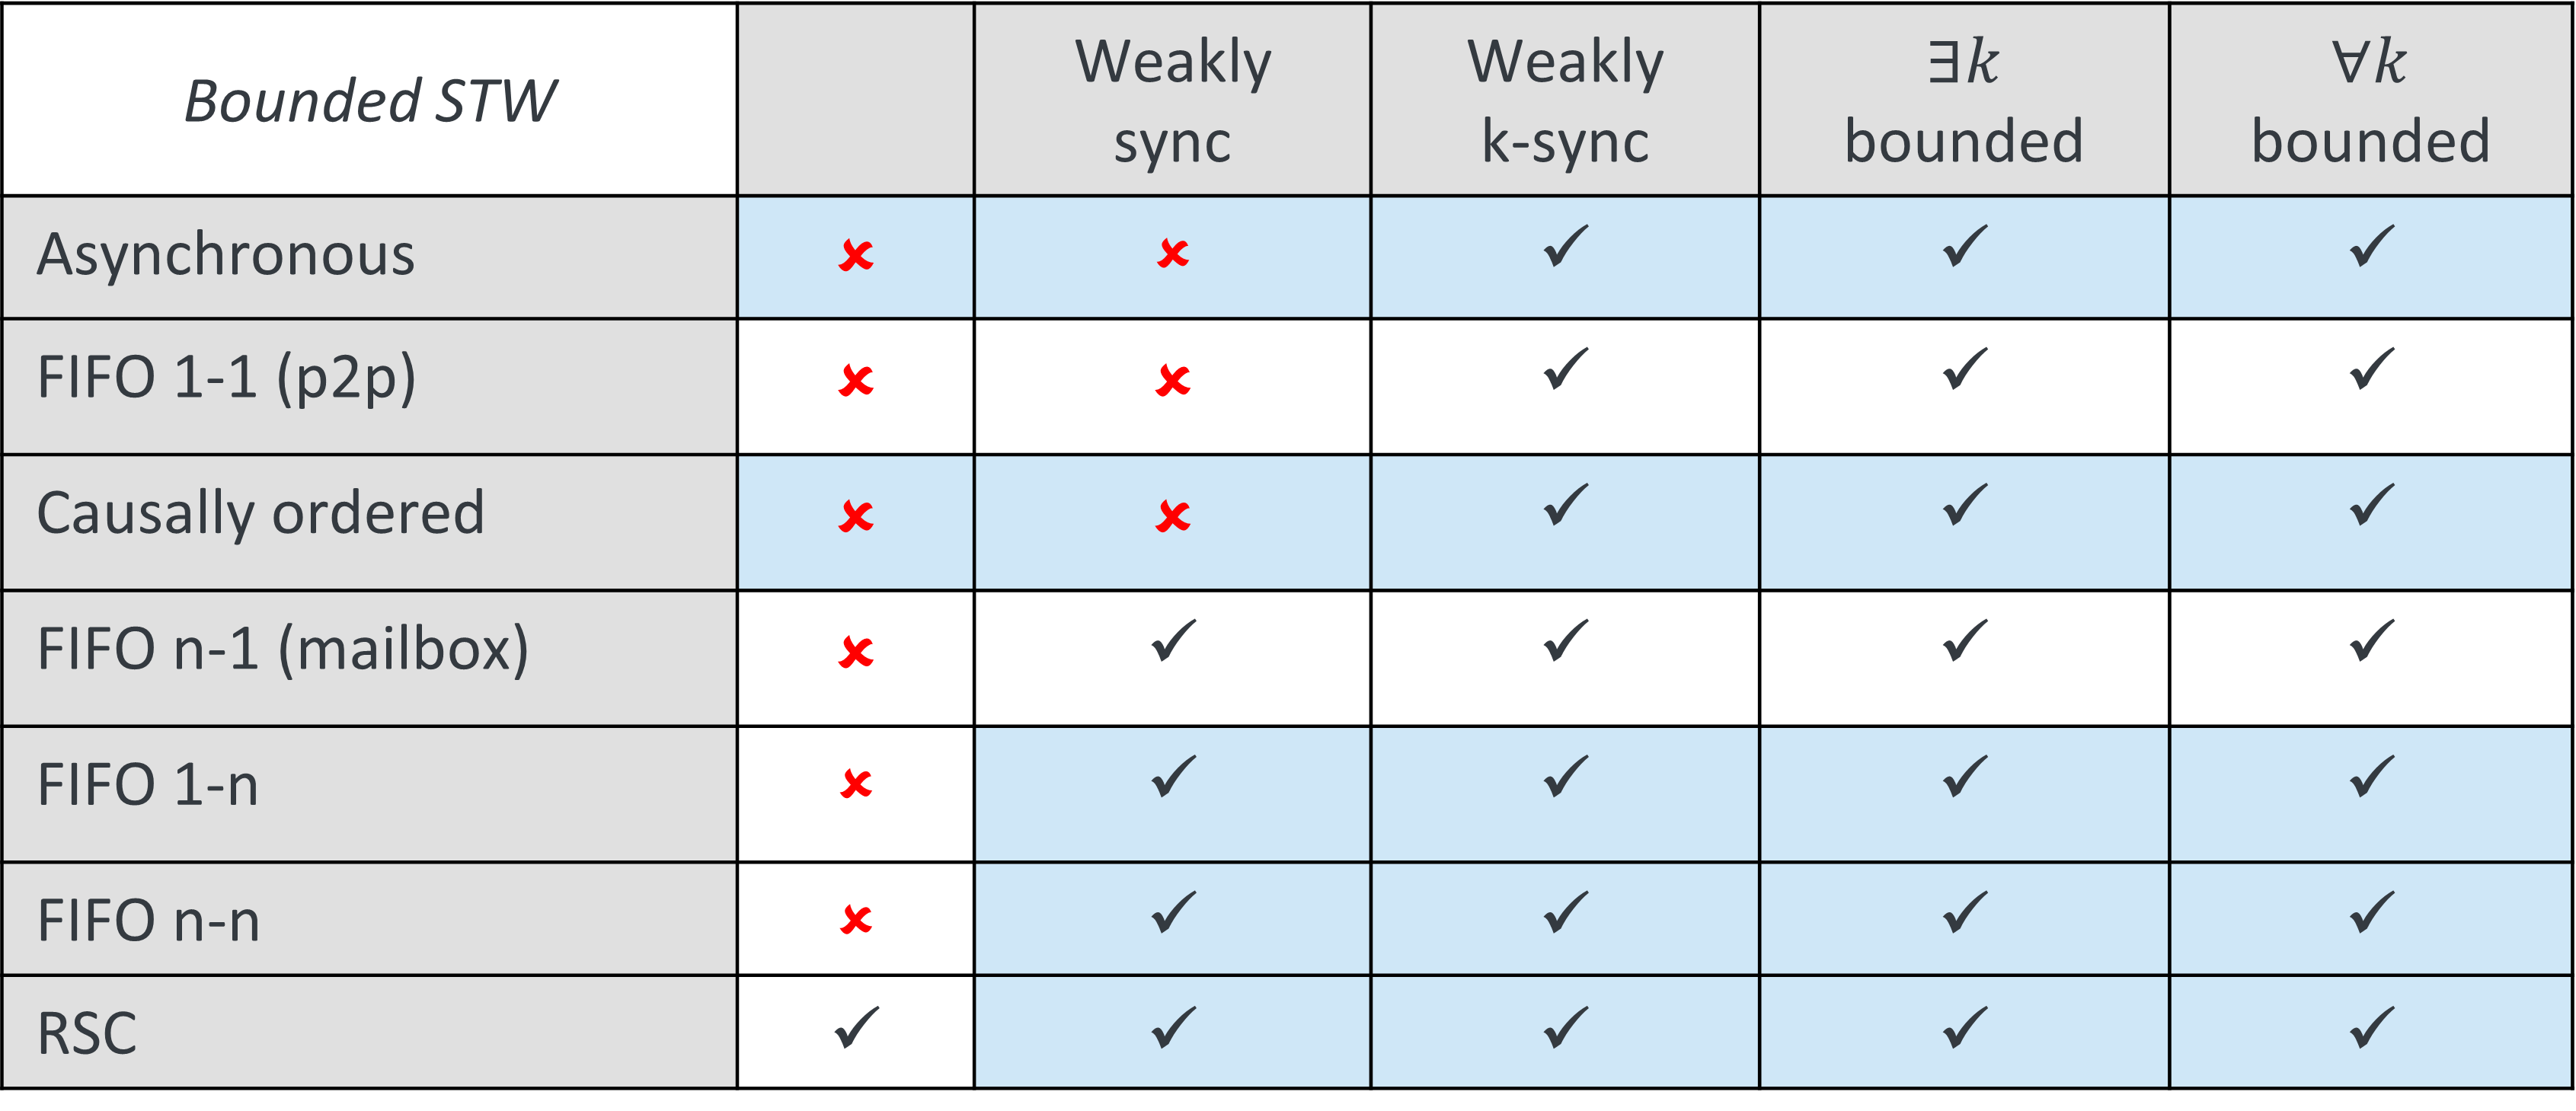
\includegraphics[width=10cm]{stw_bound}
% 	\end{center}
% \end{figure}

In this section, we show how the MSO characterisation of all of the communication
models we considered induce several decidability results for
synchronisability and bounded model-checking problems on systems of
communicating finite state machines.

A communicating finite state machine is a finite state automaton labeled with send
and receive actions; a system $\Sys$ is a finite collection of such machines.
An MSC $\msc$ is an asynchronous behaviour of $\Sys$ if every process
time line of $\msc$ is accepted by its corresponding process automaton
\ifappendix
(see Appendix~\ref{app:cfsm-def} for a formal definition of these notions).
\fi
We write $L_{\asy}(\Sys)$ to denote the set of asynchronous behaviours of $\Sys$,
and we write $L_{\comsymb}(\Sys)$ to denote the restriction of $L_{\asy}$ to $\comsymb$ MSCs,
i.e. $L_{\comsymb}(\Sys)=L_{\asy}(\Sys)\cap\MSCclassofcom{\comsymb}$.

Let $\aMSCclass$ be a class of $\MSCs$. The $\aMSCclass$-bounded model-checking problem
for the communication model $\comsymb$ is the following: given a system $\Sys$ and a MSO
specification $\amsoformula$, decide whether
$L_{\comsymb}(\Sys)\cap \aMSCclass \subseteq L(\amsoformula)$.

In the remainder, we will consider classes $\aMSCclass$ of MSCs that share the same intuition
that they only contain "almost synchronous" MSCs. So the bounded model-checking problem
corresponds to an under-approximation of the standard model-checking problem where the
system is assumed to be "almost synchronous". The question of the completeness of this under-approximaton, 
i.e. whether $L_{\comsymb}(\Sys)\subseteq \aMSCclass$, will be later
refered to as the "synchronisability problem".


Bollig~\emph{et al}~\cite{BolligFG21} introduced a general framework that allows to derive decidability results 
for the bounded model-checking and synchronizability problems
for various classes of MSCs $\aMSCclass$. The communication model is however a fixed parameter
in their framework.
In this section, we rougghly manage to make this framework parametric in the communication
model, up to several technical restrictions. The first restriction is that the communication
model, combined with the bounding class $\aMSCclass$, should enforce a bounded tree-width of the
MSCs, which is not always the case. The second restriction is that a key lemma in the framework
of  Bollig~\emph{et al} relied on the existence of "borderline violations", which was granted
by a form of prefix closure of the MSCs of a given class. However, this prefix closure property
does not hold for all communication models, and these models must be treated with specific
techniques.

\subsection{Special treewidth and bounded model-checking\label{sec:stw}}

\emph{Special treewidth} (STW)
is a graph measure that somehow indicates how close
a graph is to a tree (we may also use Courcelle's classical \emph{tree-width} instead~ \cite{Courcelle10}).
This measure or similar ones are commonly employed in verification. For instance, tree-width and split-width have been used in~\cite{MadhusudanP11} and~\cite{DBLP:conf/concur/CyriacGK12,AiswaryaGK14}, respectively, to reason about graph behaviors generated by pushdown and queue systems.
%Here we apply it to reason about MSCs.
Note that a MSC is a graph where the nodes are the events and the edges are represented by the $\procrel$ and the $\lhd$ relations.

There are several ways to define the special treewidth of a graph.
We adopt the following game-based definition from~\cite{DBLP:journals/corr/abs-1904-06942},
and, to make it more concrete, reformulate it directly on MSCs instead of graphs.
Adam and Eve play a turn based ``decomposition game'' on an MSC $\msc = (\Events, \procrel, \lhd, \lambda)$. $\msc$
Eve starts to play and does a move, which consists in the following steps:
\begin{enumerate}
	\item marking some events of $\msc$, resulting in the \emph{marked MSC fragment} $(M, U')$, where $U' \subseteq \Events$ is the subset of marked events,
	\item removing edges whose both endpoints are marked, in such a way that the resulting MSC is disconnected (i.e. there are at least two different connected components),
	\item splitting $(M, U)$ in $(M_1, U_1)$ and $(M_2, U_2)$ such that $M$ is the disjoint (unconnected) union of $M_1$ and $M_2$
	and marked nodes are inherited.
\end{enumerate}
Once Eve does her move, it is Adam's turn. Adam simply chooses one of the two marked MSC fragments, either $(M_1, U_1)$ or $(M_2, U_2)$. Now it is again Eve's turn, and she has to do a move on the marked MSC fragment that was chosen by Adam. The game continues in alternating turns between the two players until they reach a point where all the events on the current marked MSC fragment are marked.
For $k \in \N$, we say that the game is $k$-winning for Eve if she has a strategy that allows her, independently of Adam's moves, to end the game in a way that every marked MSC fragment visited during the game has at most $k+1$ marked events. The goal of Eve is to keep $k$ as low as possible. Fig.~\ref{fig:stw-ex} shows an example of a 3-winning game for the MSC in Fig.~\ref{fig:pp_ex}.

The special treewidth of an MSC is the least $k$ such that
the associated game is $k$-winning for Eve
(see for instance~\cite{DBLP:journals/corr/abs-1904-06942}).
The set of MSCs whose special treewidth is at most $k$ is denoted by $\stwMSCs{k}$. It is easy to check that trees have a special treewidth of 1.

\begin{example}
	Let $\msc$ the MSC of the Fig.~\ref{fig:pp_ex}. In this example, we show that $\msc$ has a special treewidth  $\le 3$, since Eve is able to find a strategy that leads to a 3-winning game.  We use colours to mark events. Eve starts by marking 4 events. The edges whose both endpoints are marked can be removed (dotted edges in the figure) and the graph becomes disconnected. Eve then splits the graph in 2 and Adam has to choose.
	Suppose the Adam picks the subgraph with the red and yellow events already marked (top branch in the figure). Eve can mark the third event and, by doing so, the game ends.
	Suppose Adam chooses the subgraph with the blue and green events (bottom branch). Eve marks the two nodes in the bottom, removes 3 edges, and splits the graph in two. Note that one of the two subgraphs already has all events marked, so Adam is picks the other one (top branch).
	Eve simply marks the missing event and the game ends. This is a 3-winning game for Eve since, independently of Adam's choices, we have at most 4 marked event at each step.
\end{example}
% !TEX root = ../popl-paper.tex

\begin{figure}[t]
	\begin{center}
		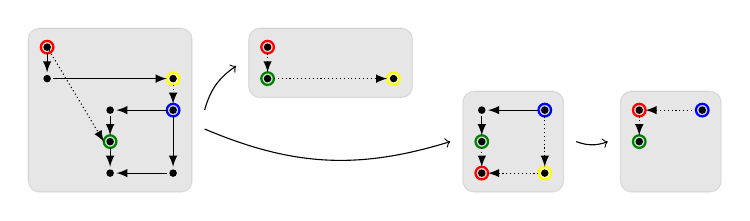
\begin{tikzpicture}[scale = .8]
			\begin{scope}
				\draw[gray,fill = gray, rounded corners, opacity=0.2] (-.3,.3) rectangle (2.3,-2.3);
				\draw[red, thick, fill = red!20] (0,0) circle (0.1);
				\draw[Green, thick, fill = Green!20] (1,-1.5) circle (0.1);
				\draw[Yellow, thick, fill = Yellow!20] (2,-.5) circle (0.1);
				\draw[blue, thick, fill = blue!20] (2,-1) circle (0.1);

				\draw[black, fill = black] (0,0) circle (.05);
				\draw[black, fill = black] (0,-.5) circle (.05);
				\draw[black, fill = black] (2,-.5) circle (.05);
				\draw[black, fill = black] (1,-1) circle (.05);
				\draw[black, fill = black] (2,-1) circle (.05);
				\draw[black, fill = black] (1,-1.5) circle (.05);
				\draw[black, fill = black] (1,-2) circle (.05);
				\draw[black, fill = black] (2,-2) circle (.05);

				\draw[>=latex, ->] (0,-.1) to (0, -.4);
				\draw[>=latex, ->,  densely dotted] (0,0) to (.9, -1.5);
				\draw[>=latex, ->] (.1,-.5) to (1.9, -.5);
				\draw[>=latex, ->,  densely dotted] (2,-.6) to (2, -.9);
				\draw[>=latex, ->] (1.9,-1) to (1.1, -1);
				\draw[>=latex, ->] (1,-1.1) to (1, -1.4);
				\draw[>=latex, ->] (1,-1.6) to (1, -1.9);
				\draw[>=latex, ->] (2,-1.1) to (2, -1.9);
				\draw[>=latex, ->] (1.9,-2) to (1.1, -2);

				\draw[->] (2.5,-1) to[bend left = 20] (3,-.3);
				\draw[->] (2.5,-1.3) to[bend right = 20] (6.4,-1.5);
				\draw[->] (8.4,-1.5) to[bend right = 20] (8.9,-1.5);


			\end{scope}
			\begin{scope}[shift = {(3.5,0)}]
				\draw[gray,fill = gray, rounded corners, opacity=0.2] (-.3,.3) rectangle (2.3,-.8);
				\draw[red, thick, fill = red!20] (0,0) circle (0.1);
				\draw[Green, thick, fill = Green!20] (0,-.5) circle (0.1);
				\draw[Yellow, thick, fill = Yellow!20] (2,-.5) circle (0.1);

				\draw[black, fill = black] (0,0) circle (.05);
				\draw[black, fill = black] (0,-.5) circle (.05);
				\draw[black, fill = black] (2,-.5) circle (.05);

				\draw[>=latex, ->, densely dotted	] (0,-.1) to (0, -.4);
				\draw[>=latex, ->, densely dotted	] (.1,-.5) to (1.9, -.5);
			\end{scope}
			\begin{scope}[shift = {(5.9,0)}]
				\draw[gray,fill = gray, rounded corners, opacity=0.2] (.7,-.7) rectangle (2.3,-2.3);
				\draw[red, thick, fill = red!20] (1,-2) circle (0.1);
				\draw[Green, thick, fill = Green!20] (1,-1.5) circle (0.1);
				\draw[Yellow, thick, fill = Yellow!20] (2,-2) circle (0.1);
				\draw[blue, thick, fill = blue!20] (2,-1) circle (0.1);

				\draw[black, fill = black] (1,-1) circle (.05);
				\draw[black, fill = black] (2,-1) circle (.05);
				\draw[black, fill = black] (1,-1.5) circle (.05);
				\draw[black, fill = black] (1,-2) circle (.05);
				\draw[black, fill = black] (2,-2) circle (.05);
				\draw[>=latex, ->] (1.9,-1) to (1.1, -1);
				\draw[>=latex, ->] (1,-1.1) to (1, -1.4);
				\draw[>=latex, ->,  densely dotted] (1,-1.6) to (1, -1.9);
				\draw[>=latex, ->,  densely dotted] (2,-1.1) to (2, -1.9);
				\draw[>=latex, ->,  densely dotted] (1.9,-2) to (1.1, -2);
			\end{scope}

			\begin{scope}[shift = {(8.4,0)}]
				\draw[gray,fill = gray, rounded corners, opacity=0.2] (.7,-.7) rectangle (2.3,-2.3);
				\draw[red, thick, fill = red!20] (1,-1) circle (0.1);
				\draw[Green, thick, fill = Green!20] (1,-1.5) circle (0.1);
				%\draw[Yellow, thick, fill = Yellow!20] (2,-2) circle (0.1);
				\draw[blue, thick, fill = blue!20] (2,-1) circle (0.1);

				\draw[black, fill = black] (1,-1) circle (.05);
				\draw[black, fill = black] (2,-1) circle (.05);
				\draw[black, fill = black] (1,-1.5) circle (.05);

				\draw[>=latex, ->,  densely dotted] (1.9,-1) to (1.1, -1);
				\draw[>=latex, ->,  densely dotted] (1,-1.1) to (1, -1.4);
				\end{scope}

		\end{tikzpicture}
	\end{center}
  \caption{Decomposition game for the MSC of Fig.~\ref{fig:pp_ex}. This is a 3-winning game for Eve.}
  \label{fig:stw-ex}
\end{figure}


Courcelle's theorem implies that the following problems is
decidable: given a MSO formula $\amsoformula$ and $k\geq 1$,
decide whether $\amsoformula$ holds for all MSCs $\msc\in\stwMSCs{k}$.
Therefore, a direct consequence of Courcelle's theorem and of our MSO characterisation
of the communication models is that bounded-model-checking is decidable.

\begin{theorem}\label{thm:bounded-model-checking}
Let $\comsymb\in\{\asy, \co, \pp, \mb, \onen, \nn, \rsc\}$ and $k\geq 1$ be fixed.
Then the following problem is decidable: given a system $\Sys$ and
a MSO specification $\amsoformula$, decide whether
$L_{\comsymb}(\Sys)\cap \stwMSCs{k}\subseteq L(\amsoformula)$.
\end{theorem}

\subsection{The synchronizability problem}

Theorem~\ref{thm:bounded_model_checking} remains true if instead of
$\stwMSCs{k}$ we bound the model-checking problem with
a class $\aMSCclass$ of MSCs that is both tree-width bounded and MSO definable.
The synchronizability problem (SP, for short) consists in understanding this bounded model-checking is complete,
i.e. whether all the behaviours generated by a given communicating system are included in this
class $\aMSCclass$, i.e whether
$\cL{\Sys} \subseteq \aMSCclass$.

\begin{definition}
Let a communication model $\comsymb$ and a class $\aMSCclass$ of MSCs be fixed. The
$(\comsymb,\aMSCclass)$-synchronisability problem is defined as follows: given a
system $\Sys$, decide whether $L_{\comsymb}(\Sys)\subseteq \aMSCclass$
\end{definition}

In \cite{BolligFG21} the authors show that, for $\comsymb = \oneone$ and $\comsymb = \none$, 
the $(\comsymb,\aMSCclass)$-synchronizability problem is decidable for several classes $\aMSCclass$. 
We generalize their result to other communication models under a slight assumption on the bounding class $\aMSCclass$.

\begin{restatable}{theorem}{thmsync}\label{thm:sync}
%	Fix finite sets $\Procs$ and $\Msg$.
	For any $\comsymb \in \{\asy, \oneone, \co, \none, \onen, \nn\}$ and
	for all MSO-definable class $\aMSCclass \subseteq \MSCs$ of MSCs,
	if $\MSCclassofcom{\comsymb}\cap\aMSCclass$ is STW-bounded,
	then the $(\comsymb,\aMSCclass)$-synchronisability problem is decidable.
\end{restatable}
Appendix~\ref{apx:sync} is entirely devoted to the proof of Theorem~\ref{thm:sync}.


In the next sections, we investigate which combinations of $\comsymb$ and $\aMSCclass$ fit the hypotheses of this theorem.
We review the classes of weakly synchronous and weakly k-synchronous inspired
by~\cite{DBLP:conf/cav/BouajjaniEJQ18},
and the classes of existentially $k$-bounded and universally $k$-bounded MSCs~\cite{DBLP:conf/dlt/GenestMK04}.

% As shown in \cite{BolligFG21}, if we have a system $\Sys$ and a STW-bounded class $\aMSCclass$, then the model-checking problem\footnote{Given $\Procs$ and $\Msg$, a communicating system $\Sys$, an MSO sentence $\phi$, do we have $\cL{\Sys} \subseteq L(\phi)?$} for $\Sys$ becomes decidable if $L(S) \subseteq \aMSCclass$; this motivates the study of the synchronizability problem.

Fig.~\ref{fig:stw-bound} summarizes the decidability results of the
$(\comsymb,\aMSCclass)$-synchronizability problem for each combination of $\comsymb$ and $\aMSCclass$ 
we will consider in the next sections.


\begin{figure}[t]
		\begin{tabular}{| c | c | c|  c| c| }
			\hline
			& Weakly  & Weakly  & $\exists$k & $\forall$k  \\
			& sync & k-sync & bounded & bounded \\
			\hline \hline
			$\asy$ &  \xmark & \cmark & \cmark & \cmark \\
			\hline
			$\oneone$  & \xmark~[1] & \cmark~[1] & \cmark~[1] & \cmark~[1] \\
			\hline
			$\co$  & \xmark & \cmark & \cmark & \cmark \\
			\hline
			$\none$ & \cmark~[1] & \cmark~[1] & \cmark~[1] & \cmark~[1] \\
			\hline
			$\onen$ & \cmark & \cmark & \cmark & \cmark \\
			\hline
			$\nn$ & \cmark & \cmark & \cmark & \cmark \\
			\hline
		%	$\rsc$ & \cmark & \cmark & \cmark & \cmark & \cmark \\
		%	\hline
		\end{tabular}
		\caption{Table summarising the (un)decidability results for the synchronisability problems (each 
		combination of a communication model $\comsymb$ and a class $\aMSCclass$ of MSCs is a different 
		synchronisability problem). 
		The symbol \xmark\;stands for undecidability and unbounded special tree-width
		of $\comsymb\cap \aMSCclass$, whereas \cmark\;stands for decidability and bounded STW
		of $\comsymb\cap \aMSCclass$.  
		[1] indicates that the result was shown by Bollig~\emph{et al}~\cite{DBLP:conf/concur/BolligGFLLS21}.}
		\label{fig:stw-bound}
\end{figure}



%%%%%% COPY-PASTE from report

% \subsection{Semantics of causal ordering}

% \newcommand{\buffers}{\vv{\text{Buf}}}
% \newcommand{\clocks}{\vv{\text{Vec}}}
% \begin{definition}
% 	Given a system $\System = (Loc_p, \delta_p, \ell^0_p)_{p\in\procSet}$ with $n$ processes, a \emph{configuration} is a tuple $(\vv{\ell},\buffers,\clocks)$, where $\vv{\ell}=(\ell_p)_{p \in \procSet}$ represents the global state of the system, $\buffers=(b_p)_{p \in \procSet}$ is a vector of buffers, with each $b_p \in \Msg^*$ representing the content of the buffer of process $p$, and $\clocks=(v_p)_{p \in \procSet}$ is a vector of Mattern-Fidge logical clocks, where each $v_p = (time_i)_{i \in \procSet}$ represents the content of the logical vector clock of process $p$.
% \end{definition}

\subsection{Weakly synchronous MSCs}

We first introduce the class of weakly synchronous MSCs. 
This is a generalization of synchronous MSCs studied 
in~\cite{DBLP:conf/cav/BouajjaniEJQ18}. 
We say an MSC is weakly synchronous if it is breakable into \emph{exchanges}, where an exchange is an MSC that allows one to schedule all 
sends before all receives. 

\begin{definition}[exchange]\label{def:weak-synchr}
Let $\msc = (\Events,\procrel,\lhd,\lambda)$ be an MSC.
We say that $\msc$ is an \emph{exchange} if
$\SendEv{\msc}$ is
a ${\le}$-downward-closed set.
\end{definition}

\noindent
\begin{minipage}[c]{10.5cm}

In other words, an exchange is an MSC $\msc$ where no send event depends on a receive event. 
If that is the case, we can find a linearization for $\msc$ where all the send events are executed before the 
receive events. Remember that $\msc_1\cdot\msc_2$ denote the vertical concatenation of MSC (see Section~\ref{sec:msc}).

\begin{definition}[weakly synchronous]\label{def:weaksync-new}
	We say that $\msc \in \MSCs$ is
	\emph{weakly synchronous} if it is of the form
	$\msc = \msc_1 \cdot \ldots \cdot \msc_n$
	such that every $\msc_i$ is an exchange.
\end{definition}

\begin{example}\label{example:msc_W}
	Consider the MSC $\mscW$ in Fig.~\ref{fig:msc_W}. It is is weakly synchronous. Indeed, $\amessage_1$, $\amessage_2$, and $\amessage_5$ are independent and can be put alone in an exchange. Repetitions of $\amessage_3$ and $\amessage_4$ are interlaced, but they constitute an exchange, as we can do all sends and then all receptions.
\end{example}
\end{minipage}
\hfill
\begin{minipage}[c]{3cm}
	\begin{center}
	  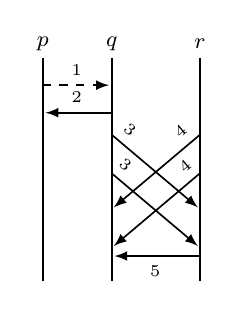
\begin{tikzpicture}[>=stealth,node distance=3.4cm,shorten >=1pt,
	  every state/.style={text=black, scale =0.6}, semithick,
		font={\fontsize{8pt}{12}\selectfont}]

	\begin{scope}[shift = {(8,0.75)}, scale = 0.7]
	  %MACHINES
	  \draw (0,1.25) node{$q$} ;
	  \draw (1.6,1.25) node{$r$} ;
	  \draw (-1.25,1.25) node{$p$} ;
	  \draw (0,1) -- (0,-3.1) ;
	  \draw (1.6,1) -- (1.6,-3.1);
	  \draw (-1.25,1) -- (-1.25,-3.1);

	  %MESSAGES
	  \draw[>=latex,->, dashed] (-1.25, 0.5) -- (0, 0.5) node[ above, midway] {$\amessage_1$};
	  \draw[>=latex,->] (0, 0) -- (-1.25, 0) node[ above, midway] {$\amessage_2$};


	  \draw[>=latex,->] (0, -0.4) -- (1.6, -1.75) node[pos=0.1, sloped, above] {$\amessage_3$};
	  \draw[>=latex,->] (0, -1.1) -- (1.6, -2.45) node[pos=0.05, sloped, above] {$\amessage_3$}; %{$\amessage_1'$};
	  %\draw[>=latex,->, dashed] (0, -2.5) -- (1.25, -3.25) node[pos=0.55, sloped, above] {$\amessage_1''$};

	  \draw[>=latex,->] (1.6, -0.4) -- (0, -1.75) node[pos=0.1, sloped, above] {$\amessage_4$};
	  \draw[>=latex,->] (1.6, -1.1) -- (0, -2.45) node[pos=0.05, sloped, above] {$\amessage_4$}; %{$\amessage_2'$};
	  %\node[rotate = 90, left]at (1.13, -0.65) {$\cdots$};
	  %\node[rotate = -90, right]at (0.1, -0.65) {$\cdots$};

	  \draw[>=latex,->] (1.6, -2.6) -- (0, -2.6) node[ below, midway] {$\amessage_5$};


	\end{scope}

	\end{tikzpicture}
	\captionof{figure}{MSC $\mscW$}
	\label{fig:msc_W}
	\end{center}
\end{minipage}

In \cite{BolligFG21} it is shown that, for the class of weakly synchronous MSCs, 
the synchronisability problem is undecidable for $\comsymb = \oneone$, but decidable for $\comsymb = \oneone$.
Here we investigate the decidability of weak synchronability for other 
communication models. We first show that weak synchronisability 
is undecidable for causally ordered communication. 

\begin{restatable}{theorem}{thmCoWeakSync}\label{thm:co-weak-sync}
	The following problem is undecidable:
	Given finite sets $\Procs$ and $\Msg$ as well as a communicating system $\System$,
	is every MSC in $\coL{\System}$ weakly synchronous?
\end{restatable}

For $\onen$ and $\nn$, on the other hand, weak synchronisability is decidable. 

\begin{proposition}\label{thm:weak-sync}
	Let $\comsymb \in \{$$\onen, $ $\nn\}$.
	The following problem is decidable:
	given finite sets $\Procs$ and $\Msg$ as well as a communicating system $\System$,
	is every MSC in $\cL{\System}$ weakly synchronous?
\end{proposition}

\begin{proof}
	The claim follows from Theorem~\ref{thm:sync}. We only detail the proof
	for the $\onen$ case (the other is identical). To apply Theorem~\ref{thm:sync}, we need to check that
	(1) the class $\aMSCclass_{ws}$ of weakly synchronous MSCs is MSO definable, and (2)
	$\aMSCclass_{ws}\cap \MSCclassofcom{\onen}$ is STW-bounded. 
	(1) has been proved by Bollig~\emph{et al}~\cite{DBLP:conf/concur/BolligGFLLS21}. For (2),
	it follows from the fact that $\MSCclassofcom{\onen}\subseteq \MSCclassofcom{\mb}$ (Prop~\ref{prop:onen_mb_unmatched}) and the fact $\aMSCclass_{ws}\cap \MSCclassofcom{\mb}$ is STW-bounded 
	(see~\cite{DBLP:conf/concur/BolligGFLLS21}).

	\etienne{Better cite CONCUR paper to say where to look for the proof (cite[Thm truc]\{paper bidule\}).}
	% We will consider $\comsymb = \onen$; the proof for $\comsymb = \nn$ follows the same steps. We would like to know if every MSC in $\onenL{\System}$ is in the class of weakly synchronous MSCs. Since every MSC in $\onenL{\System}$ is a $\onen$ MSC, we can equivalently restrict the problem to the class of weakly synchronous MSCs that are also $\onen$ MSCs. Let $\aMSCclass$ be the class of $\onen$ weakly synchronous MSCs; we show that $\aMSCclass$ is MSO-definable and STW-bounded, which implies the decidability of $SP$ for Theorem~\ref{thm:sync}. The class of weakly synchronous MSCs was shown to be MSO-definable in \cite{BolligFG21}; to be precise, their characterization is for $\oneone$ weakly synchronous MSCs (since their definition of MSC is equivalent to our definition of $\oneone$ MSC), but it also works for (asynchronous) weakly synchronous MSCs. We showed in Section~\ref{sec:MSO} that $\onenMSCs$ is MSO-definable; it follows that the class of $\onen$ weakly synchronous MSCs is also MSO-definable (we just take the conjuction of the the two formulas). The class of $\none$ weakly synchronous MSCs was shown to be STW-bounded in \cite{BolligFG21}, and since $\onenMSCs \subset \mbMSCs$, we also have that the class of $\none$ weakly synchronous MSCs has a bounded special treewidth. 
\end{proof}

\subsection{Weakly \texorpdfstring{$k$}{k}-synchronous MSCs}

The undecidability result for some of the communication models motivates the study of other classes. Here we present weakly $k$-synchronous MSCs (\cite{BolligFG21}), which are a variant of weakly synchronous MSCs where the number of messages sent per exchange is at most $k$.

\begin{definition}[$k$-exchange]\label{def:weak-k-synchr}
Let $\msc = (\Events,\procrel,\lhd,\lambda)$ be an MSC
and $k \in \N$.
We call $\msc$ a $k$-\emph{exchange} if
$\msc$ is an exchange and $|\SendEv{\msc}| \le k$.
\end{definition}

\begin{definition}[weakly $k$-synchronous]\label{def:weaksync}
Let $k \in \N$.
We say that $\msc \in \MSCs$ is
weakly $k$-synchronous if it is of the form
$\msc = \msc_1 \cdot \ldots \cdot \msc_n$
such that every $\msc_i$ is a $k$-exchange.
\end{definition}

\noindent
\begin{minipage}[c]{10.5cm}
	\begin{example}
	MSC $\mscweakSexist$ in Fig.~\ref{fig:msc_weak_S_exist} is weakly $1$-synchronous, as it can be
	decomposed  into three \kE{1}s (the decomposition is depicted by the
	horizontal dashed lines). We remark that $\mscweakSexist \in
	\mbMSCs$. Note that there is a p2p linearization that respects the decomposition.
	On the other hand, a mailbox linearization needs to reorganize actions from different MSCs: the sending of
	$\msg_3$ needs to be done before the sending of $\msg_1$. Note that $\mscweakuniver$ in
	Fig.~\ref{fig:msc_weak_univer} is also weakly $1$-synchronous.
	\end{example}
\end{minipage}
	\hfill
\begin{minipage}[c]{3cm}
\begin{center}

	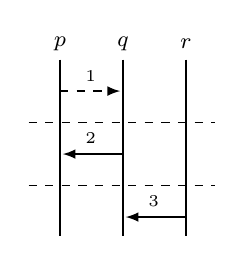
\begin{tikzpicture}[>=stealth,node distance=3.4cm,shorten >=1pt,
		every state/.style={text=black, scale =0.7}, semithick,
		font={\fontsize{8pt}{12}\selectfont}, scale = 0.8]

	  %MACHINES
	  \draw (0,0) node{$p$} ;
	  \draw (1,0) node{$q$} ;
	  \draw (2,0) node{$r$} ;
	  \draw (0,-0.25) -- (0,-3.1) ;
	  \draw (1,-0.25) -- (1,-3.1);
	  \draw (2, -0.25) -- (2, -3.1) ;
	  %MESSAGES
	  \draw[>=latex,->, dashed] (0,-0.75) -- (1, -0.75) node[midway,above]{$\amessage_1$};

	  \draw[>=latex,->] (1, -1.75) -- (0, -1.75) node[midway, above] {$\amessage_2$};
	  %\draw (0.5,-1.7) node{$\cdots$};
	  %\draw[>=latex,->] (1, -2.25) -- (0, -2.25) node[midway, above] {$\amessage_2$};

	  \draw[>=latex,->] (2,-2.75) -- (1,-2.75) node[midway, above] {$\amessage_3$};
	%\end{scope}
	  \draw[dashed] (-0.5,-1.25) -- (2.5,-1.25) ;
	  \draw[dashed] (-0.5,-2.25) -- (2.5,-2.25) ;


	\end{tikzpicture}
	\captionof{figure}{MSC $\mscweakSexist$}
	\label{fig:msc_weak_S_exist}

\end{center}
\end{minipage}

As for weakly synchronous MSCs, the class of weakly $k$-synchronous MSCs was already shown to be MSO-definable and STW-bounded in \cite{BolligFG21}, and these results still hold even for our definition of MSC. A direct application of Theorem~\ref{thm:sync} shows that, for weakly $k$-synchronous MSCs, $SP$ is decidable for all communication models.

\begin{proposition}\label{thm:weak-k-sync}
	Let $\comsymb \in \{$$\asy, $ $\oneone, $ $\co, $ $\none, $ $\onen, $ $\nn\}$.
	The following problem is decidable:
	given finite sets $\Procs$ and $\Msg$ as well as a communicating system $\System$,
	is every MSC in $\cL{\System}$ weakly $k$-synchronous?
\end{proposition}
\begin{proof}
	The class $\aMSCclass$ of weakly $k$-synchronous MSCs is MSO-definable and STW-bounded. $SP$ is decidable for Theorem~\ref{thm:sync}.
\end{proof}

\subsection{Existentially bounded MSCs}

We move now to existentially $k$-bounded MSCs, which have been studied extensively in literature \cite{DBLP:conf/fossacs/LohreyM02,DBLP:conf/dlt/GenestMK04,GKM07,BolligFG21}. These  kind of MSCs represent the behaviour of systems that can be realized with bounded channels, i.e. channels where at most $k$ messages can transit at any moment in time. For our definition of $k$-bounded MSCs, we suppose that there is a channel $(p,q)$ for any pair of processes such that $p$ sends messages to $q$ (there is a different channel for messages sent by $q$ to $p$). Intuitively, we say that an MSC is existentially $k$-bounded if it has linearization where, at any moment in time, there are no more than $k$ messages in any channel. Such a linearization will be referred to as a $k$-\emph{bounded linearization}. We give formal definitions below.

\begin{definition}\label{def:lin_k_bounded}
	Let $\msc = (\Events,\procrel,\lhd,\lambda) \in \MSCs$ and $k \in \N$.
	A linearization $\linrel$ of $\msc$ is called
	$k$-\emph{bounded} if, for all $e \in \SendEv{\msc}$, with $\lambda(e) = \sact{p}{q}{\msg}$, we have
	\[
	\sametype{e}{\pqsAct{p}{q}}{\linrel} - \sametype{e}{\pqrAct{p}{q}}{\linrel} \le k
	\]
\end{definition}
\noindent where $\sametype{e}{A}{\rel} = |\{f \in \Events \mid (f,e) \in \rel$ and $\lambda(f) \in A\}|$.
For instance, $\sametype{e}{\pqsAct{p}{q}}{\linrel}$ denotes the number of send events from $p$ to $q$ that occured before $e$ according to $\linrel$\footnote{Note that, since $\linrel$ in reflexive, $e$ itself is counted in $\sametype{e}{\pqsAct{p}{q}}{\linrel}$}.

\begin{definition}[Existentially bounded MSC]\label{def:ek_bounded_msc}
	Let $\msc = (\Events, \rightarrow, \lhd, \lambda) \in \asMSCs$ and $k \in \mathbb{N}$. We call $\msc$ \emph{existentially $k$-bounded} ($\exists k$-bounded) if it has a $k$-bounded linearization.
\end{definition}
We now look at the definitions of $\oneone$ $\exists k$-bounded MSCs and causally ordered $\exists k$-bounded, which are quite straightforward.

\noindent
\begin{minipage}[c]{10.5cm}
\begin{example}
  MSC $\mscexist$ in Fig.~\ref{fig:msc_exist}
  is existentially $1$-bounded, as witnessed by the linearization $!2\;!1\;!3\;?3\;?1\;!1\;?2\;!3\;?3 \ldots$
  Note that $\mscexist$ is not weakly synchronous as we cannot divide it into exchanges.
\end{example}
\end{minipage}
\begin{minipage}[c]{3cm}
	\begin{center}
		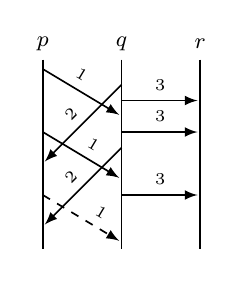
\begin{tikzpicture}[>=stealth,node distance=3.4cm,shorten >=1pt,
		every state/.style={text=black, scale =0.7}, semithick,
		  font={\fontsize{8pt}{12}\selectfont}]
	  \begin{scope}[shift = {(0,0)}, scale = 0.8]
		% \draw (1.25, -4.75) node{\textbf{(a)}};
		% \draw (4.5, -4.75) node{\textbf(b)};

		%MACHINES
		\draw (0,-0.1) node{$p$} ;
		\draw (1.25,-0.1) node{$q$} ;
		\draw (2.5,-0.1) node{$r$} ;
		\draw (2.5, -0.35) -- (2.5, -3.4) ;
		\draw (0,-0.35) -- (0,-3.4) ;
		\draw (1.25,-0.35) -- (1.25,-3.4);
		%MESSAGES

		\draw[>=latex,->] (0, -0.5) -- (1.25, -1.25) node[pos=0.4, sloped, above] {$\amessage_1$};
		\draw[>=latex,->] (0, -1.5) -- (1.25, -2.25) node[pos=0.55, sloped, above] {$\amessage_1$};
		\draw[>=latex,->, dashed] (0, -2.5) -- (1.25, -3.25) node[pos=0.65, sloped, above] {$\amessage_1$};

		\draw[>=latex,->] (1.25, -0.75) -- (0, -2) node[pos=0.5, sloped, above] {$\amessage_2$};
		\draw[>=latex,->] (1.25, -1.75) -- (0, -3) node[pos=0.5, sloped, above] {$\amessage_2$};


		\draw[>=latex,->] (1.25, -1) -- (2.5, -1) node[midway, above] {$\amessage_3$};
		\draw[>=latex,->] (1.25, -1.5) -- (2.5, -1.5) node[midway, above] {$\amessage_3$};
		\draw[>=latex,->] (1.25, -2.5) -- (2.5, -2.5) node[midway, above] {$\amessage_3$};

		%\draw (0.6, -3.35) node{$\cdots$};
		%\draw (1.9, -3.35) node{$\cdots$};
	  \end{scope}
			% \begin{scope}[shift = {(3,0)}, scale = 0.8]
			%   % \draw (0.5, -4) node{\textbf{(b)}};
			%   %MACHINES
			%   \draw (0,0) node{$p$} ;
			%   \draw (1,0) node{$q$} ;
			%   \draw (0,-0.25) -- (0,-3.5) ;
			%   \draw (1,-0.25) -- (1,-3.5);
			%   %MESSAGES
			%
			%    \draw[>=latex,->] (0, -0.75) -- (1, -0.75) node[midway, above] {$\amessage_1$};
			%    \draw[>=latex,->] (1, -1.5) -- (0, -1.5) node[midway, above] {$\amessage_2$};
			%    \draw[>=latex,->] (0, -2.25) -- (1, -2.25) node[midway, above] {$\amessage_1$};
			%    \draw[>=latex,->] (1, -3) -- (0, -3) node[midway, above] {$\amessage_2$};
			%
			%
			%   % \draw (0.5, -3.25) node{$\cdots$};
			% \end{scope}
			  \end{tikzpicture}
	  \captionof{figure}{MSC $\mscexist$}
	  \label{fig:msc_exist}
	\end{center}
\end{minipage}

\begin{definition}
	An MSC $\msc$ is \emph{$\oneone$ existentially $k$-bounded} ($\oneone$-$\exists k$-bounded) if it is a $\oneone$ MSC and it is also existentially $k$-bounded.
\end{definition}
\begin{definition}
	An MSC $\msc$ is \emph{causally orderered existentially $k$-bounded} ($\cosymb$-$\exists k$-bounded) if it is a causally ordered MSC and it is also existentially $k$-bounded.
\end{definition}

When moving on to the other communication models, the definitions are not as straightforward. For instance, the definition of $\none$ $\exists k$-bounded MSC should require that there exists a $k$-bounded linearization that is also a $\none$ linearization, not just any linearization. Recall that an MSC is a $\none$ MSC if it has at least one $\none$ linearization, which represents a sequence of events that can be executed by a $\none$ system. Following this intuition, we want one of these $\none$ linearizations to be $k$-bounded, not just any linearization.

\begin{definition}
	An MSC $\msc$ is \emph{$\none$ existentially $k$-bounded} ($\none$-$\exists k$-bounded) if it has a $k$-bounded $\none$ linearization.
\end{definition}
% \davide{This paragraph depends on how we choose to formally define the mailbox communication model... we could go for a (i) single incoming channel, or (ii) just an enforcing of the delivery of messages by the transport layer.}
% It should be noted that, for a $k$-bounded mailbox linearization, it is not necessarily true that at any time we have at most $k$ messages in each channel. Recall that in the mailbox communication architecture every process has a single incoming channel, but the Definition~\ref{def:lin_k_bounded} of $k$-bounded linearization considers the number of pending messages between each pair $(p,q)$ of processes. Let $n$ be the number of processes. We can say that, for a $k$-bounded mailbox linearization, we have at most $k(n-1)$ messages in each channel at any moment (because each process can have at most $k$ pending messages coming from any of the other $n-1$ processes).
% \davide{An example would be nice.}

\begin{definition}
	An MSC $\msc$ is \emph{$\onen$ existentially $k$-bounded} (onen-$\exists k$-bounded) if it has a $k$-bounded $\onen$ linearization.
\end{definition}

\begin{definition}
	An MSC $\msc$ is \emph{$\nn$ existentially $k$-bounded} (nn-$\exists k$-bounded) if it has a $k$-bounded $\nn$ linearization.
\end{definition}

We show that each of the $\exists k$-bounded classes of MSCs presented so far is MSO-definable and STW-bounded. We then derive the decidability of $SP$ in a similar way to what we did in the proof of Proposition~\ref{thm:weak-sync} for weakly synchronous MSCs.

\paragraph*{MSO-definability}

Here we will investigate the MSO-definability of all the variants of $\exists k$-bounded MSCs, starting from the most general class of $\exists k$-bounded MSCs.
Following the approach taken in \cite{DBLP:conf/fossacs/LohreyM02}, we introduce a binary relation $\relb$ ($\linrel_b$ in their work) associated with a given bound $k$ and an MSC $\msc$. Let $k \ge 1$ and $\msc$ be a fixed MSC: we have $r \relb s$ if, for some $i \ge 1$ and some channel ($p$,$q$)\footnote{Recall that ($p,\,q$) is a channel where messages are sent by $p$ and received by $q$.}:
\begin{enumerate}\itemsep=0.5ex
	\item $r$ is the $i$-th receive event (executed by $q$).
	\item $s$ is the ($i+k$)-th send event (executed by $p$).
\end{enumerate}
Note that, for any two events $s$ and $r$ such that $r \relb s$, every linearization of $\msc$ in which $r$ is executed after $s$ cannot be $k$-bounded. Intuitively, we can read $r \relb s$ as "$r$ has to be executed before $s$ in a $k$-bounded linearization". A linearization $\linrel$ that respects $\relb$ (i.e. $\relb \,\subseteq\, \linrel$) is $k$-bounded.\davide{An example could be nice.} In \cite{DBLP:conf/fossacs/LohreyM02} it was shown that an MSC is $\exists k$-bounded if and only if the relation $\le \cup \relb$ is acyclic. Since $\le$ and acyclicity are both MSO-definable, it suffices to find an MSO formula that defines the $\relb$ relation to claim the MSO-definability of $\exists k$-bounded MSCs. Unfortunately, $\relb$ is not MSO-definable because MSO logic cannot be used to "count" for an arbitrary $i$. For this reason, we introduce a similar MSO-definable binary relation $\relbAsy$, and we show that an MSC $\msc$ is $\exists k$-bounded MSC iff $\le \cup \relbAsy$ is acyclic and another condition holds. Let $k \ge 1$ and $\msc$ be a fixed MSC; we have $r \relbAsy s$ if, for some $i \ge 1$ and some channel ($p$,$q$):
\begin{itemize}\itemsep=0.5ex
	\item There are $k+1$ send events $(s_1, \dots, s_k, s)$, where at least one is matched, such that $s_1 \procrel^+ \dots \procrel^+ s_k \procrel^+ s$.
 	\item $r$ is the first receive event for the matched send events among $s_1, \dots, s_k, s$.
\end{itemize}

\begin{proposition}\label{prop:asy_ek_def_alt}
	An MSC $\msc$ is $\exists k$-bounded if and only if $\le \cup \relbAsy$ is acyclic and, for each channel ($p$,$q$), there are at most $k$ unmatched send events.
\end{proposition}
\begin{proof}
	($\Rightarrow$) Suppose $\msc$ is $\exists k$-bounded, which by definition means there is at least one $k$-bounded linearization $\linrel$. Firstly, notice that every MSC that has more than $k$ unmatched send events in any channel cannot be an $\exists k$-bounded MSC. We already know that $\le \subseteq \linrel$, and we will show show that also $\relbAsy \subseteq \linrel$. This implies that $\le \cup \relbAsy$ is acyclic, otherwise we would not be able to find a linearization $\linrel$ that respects both $\le$ and $\relbAsy$. Suppose, by contradiction, that $\relbAsy \nsubseteq \linrel$, i.e. there are two events $r$ and $s$ such that $r \relbAsy s$ and $s \linrel r$. By definition of $\relbAsy$, there are $k$ send events in a channel ($p$,$q$) that are executed before $s$, and whose respective receive events happens after $r$. If $s$ is executed before $r$ in the linearization, there will be $k+1$ messages in channel (i.e. $\linrel$ is not a $k$-bounded linearization). We reached a contradiction, hence $\relbAsy \subseteq \linrel$ and $\le \cup \relbAsy$ is acyclic.\newline
	($\Leftarrow$) Suppose $\le \cup \relbAsy$ is acyclic and, for each channel ($p$,$q$), there are at most $k$ unmatched send events. If $\le \cup \relbAsy$ is acyclic, we are able to find at least one linearization $\linrel$ for the partial order $(\le \cup \relbAsy)^\ast$. We want to show that this linearization is $k$-bounded. By contradiction, suppose $\linrel$ is not $k$-bounded, i.e. we are able to find $k+1$ send events $s_1 \procrel^+ \dots \procrel^+ s_k \procrel^+ s$ on a channel ($p$,$q$), such that $s$ is executed before any of the respective receive events takes place. There are two possible scenarios:
	\begin{itemize}\itemsep=0.5ex
		\item Suppose all the $k+1$ send events are unmatched. This is impossible, since we supposed that there are at most $k$ unmatched send events for any channel.
		\item Suppose there is at least one matched send event between the $k+1$ sends. Let the first matched send event be $s_i$ and let $r$ be the receive event that is executed first among the receive events for these $k+1$ sends. By hypothesis, $s \linrel r$. However, according to the definition of $\relbAsy$, we must have $r \relbAsy s$. We reached a contradiction, since we cannot have that $s$ happens before $r$ in a linearization for the partial order $(\le \cup \relbAsy)^\ast$, if $r \relbAsy s$.
	\end{itemize}
\end{proof}

\noindent According to Proposition~\ref{prop:asy_ek_def_alt}, we can write the MSO formula the defines $\exists k$-bounded MSCs as
\[
\Psi_{\exists k}=
acyclic(\le \cup \relbAsy) \;\wedge\;
\neg \left(
	\exists s_1 \dots s_{k+1}. s_1 \procrel^+ \dots \procrel^+ s_{k+1} \;\wedge \;
	allSends\_p\_q(k+1) \;\wedge\; allUnm
\right)
\]
\[
allSends\_p\_q (t) =
\bigvee_{\substack{p \in \Procs, q \in \Procs}}\;
\bigwedge_{s \in {s_1, ..., s_{t}}}\;
\bigvee_{a \in \pqsAct{p}{q}}
(\lambda(s) = a)
\]
\[
allUnm = \bigwedge_{s \in {s_1, ..., s_{k+1}}}(\neg \mathit{matched}(s))
\]
where $acyclic(\le \cup \relbAsy)$ is an MSO formula that checks the acyclicity of $\le \cup \relbAsy$, and the $\relbAsy$ relation can be defined as
\[
r \relbAsy s= \exists s_1 \dots s_{k+1}. \left(
\begin{array}{rl}
	& s_1 \procrel^+ \dots \procrel^+ s_{k+1} \;\wedge\;
	allSends\_p\_q(k+1) \;\wedge\; \\
	& \exists r. (\bigvee_{s \in {s_1, ..., s_{k+1}}}s \lhd r) \;\wedge\;
	\bigwedge_{e \in {s_1, ..., s_{k+1}}}(\exists f.e \lhd f \implies r \procrel^* f) \\
\end{array}
\right)
\]

\medskip

It follows that, given $k \in \N$, the set of existentially $k$-bounded MSCs is MSO-definable. Causally ordered and $\oneone$ existentially $k$-bounded MSCs are clearly MSO-definable by definition, since we already showed that $\oneone$ MSCs, causally ordered MSCs, and existentially $k$-bounded MSCs are all MSO-definable. Recall that we introduced the $\relbAsy$ relation because the $\relb$ relation introduced in \cite{DBLP:conf/fossacs/LohreyM02} was not MSO-definable for asynchronous communication. However, when considering $\oneone$ communication\footnote{And also all of the other communication models, because of the hierarchy shown in Section~\ref{sec:hierarchy}}, $\relb$ becomes MSO-definable; the FIFO behaviour ensures that, for any channel $(p,q)$, the $i$-th matched send event of $p$ matches with the $i$-th receive event of $q$. This allows us to define $r \relb s$ as:
\[
r \relb s=\exists s_1. \dots \exists s_k.\left(
allSends\_p\_q(k)
\;\wedge\; s_1\procrel s_2\procrel\dots
\procrel s_k\procrel s
\;\wedge\; s_1 \lhd r
\right)
\]
Recall that an MSC $\msc$ is $\none$-$\exists k$-bounded if has a linearization that is both $\none$ and $\exists k$-bounded. A linearization $\linrel$ is $\none$ if $\msc$ is $\none$ and $\linrel$ is a linear extension of the partial order $\mbpartial$, i.e. $\mbpartial \;\subseteq\; \linrel$. A linearization $\linrel$ is $\exists k$-bounded if $\relb \;\subseteq\; \linrel$. It follows that a linearization $\relb$ is $\none$-$\exists k$-bounded if $(\mbpartial \cup \relb) \;\subseteq\; \linrel$. Such a linerization exists only if $\mbpartial \cup \relb$ is acyclic\footnote{If $\mbpartial \cup \relb$ is acyclic, its transive closure always exists and it is a partial order, hence we are always able to find a linear extension.}. The characterization for onen-$\exists k$-bounded MSCs and nn-$\exists k$-bounded is very similar. Below the formal definitions.

\begin{proposition}\label{prop:ek-mso}
	An MSC $\msc$ is $\none$-$\exists k$-bounded iff the relation $\mbpartial \cup \relb$ is acyclic.\\
	An MSC $\msc$ is onen-$\exists k$-bounded iff the relation $\onenpartial \cup \relb$ is acyclic.\\
	An MSC $\msc$ is nn-$\exists k$-bounded iff the relation $\bowtie \cup \relb$ is acyclic.
\end{proposition}

The MSO-definability of all the variants of $\exists$k-bounded MSCs directly follows from Proposition~\ref{prop:ek-mso}, since all of these relations were shown to be MSO-definable.

\paragraph*{Special treewidth}

In \cite[Lemma 5.37]{DBLP:journals/corr/abs-1904-06942} it was shown that the special treewidth of existentially $k$-bounded MSCs is bounded by $k\,|\Procs|^2$, for $k \ge 1$. Actually, STW-boundness was shown for the more general class of Concurrent Behaviours with Matching ($\mathsf{CBM}$), but the result is still valid since $\asMSCs \subset \mathsf{CBM}$. The special treewidth of the other classes of $\exists k$-bounded MSCs is also bounded, since they are clearly subclasses of $\exists k$-bounded MSCs.

\subsection{Universally bounded MSCs}

An MSC is existentially $k$-bounded if it has a $k$-bounded linearization. We call an MSC universally $k$-bounded MSCs if all of its linearizations are $k$-bounded, hence the name "universally".

\begin{definition}[Universally bounded MSC]\label{def:uk_bounded_msc}
	Let $\msc = (\Events, \rightarrow, \lhd, \lambda) \in \asMSCs$ and $k \in \mathbb{N}$. We call $\msc$ \emph{universally $k$-bounded} ($\forall k$-bounded) if all of its linearizations are $k$-bounded.
\end{definition}
\begin{definition}
	An MSC $\msc$ is \emph{\pp universally $k$-bounded} (\pp-$\forall k$-bounded) if it is a \pp MSC and it is also universally $k$-bounded.
\end{definition}
\begin{definition}
	An MSC $\msc$ is \emph{causally orderered universally $k$-bounded} ($\cosymb$-$\forall k$-bounded) if it is a causally ordered MSC and it is also universally $k$-bounded.
\end{definition}

As for the existential case, the definitions for the other communication models are not as straightforward. For instance, the definition of $\none$ $\forall k$-bounded MSC should require that all the $\none$ linearizations of the MSC are $k$-bounded, but we say nothing about linearizations that are not $\none$. The same goes for the $\onen$ and $\nn$ communication models.

\begin{definition}
	An MSC $\msc$ is \emph{mailbox universally $k$-bounded} (mb-$\forall k$-bounded) if it is a mailbox MSC and all of its mailbox linearizations are $k$-bounded.
\end{definition}
\begin{definition}
	An MSC $\msc$ is \emph{$\onen$ universally $k$-bounded} (1n-$\forall k$-bounded) if it is a $\onen$ MSC and all of its $\onen$ linearizations are $k$-bounded.
\end{definition}

% \subsubsection{Hierarchy}

% \davidequestion{I think that this section, albeit interesting, might be removed...}
% In this section we will investigate the relations between the various classes of universally $k$-bounded MSCs that we introduced. From their definition, it is quite straightforward to see that $\coUk \subseteq \ppUk \subseteq \asUk$. The set of mailbox universally $k$-bounded MSCs, however, does not fit in this hierarchy. Recall that an MSC is mb-$\forall k$-bounded if all of its mailbox linearizations are $k$-bounded, but the definition does not say anything about non-mailbox linearizations. It can be the case that an MSC has a bound $k$ for its mailbox linearizations, but a higher bound $k'$ for non-mailbox linearizations. Fig.~\ref{fig:mb_uk} shows an MSC $\msc$ which is mb-$\forall 1$-bounded, but $\forall 2$-bounded. According to the mailbox semantics, a mailbox linearization of $\msc$ has to respect the order $!m_1 \mbrel\, !m_3 \mbrel\, !m_4$. Note that all mailbox linearizations are $1$-bounded, but we are able to find a non-mailbox linearization that is 2-bounded, such as $!m_1 \linrel\, !m_4 \linrel\, ?m_1 \linrel\, !m_2 \linrel\, ?m_2 \linrel\, !m_3 \linrel\, !m_4 \linrel\, ?m_3 \linrel\, ?m_4$.

% \begin{figure}[h]
% \begin{center}
% \begin{tikzpicture}
% 	\newproc{0}{p}{-1.9};
% 	\newproc{1}{q}{-1.9};
% 	\newproc{2}{r}{-1.9};

% 	\newmsgml{0}{1}{-0.5}{1}{0.5}{black};
% 	\newmsgml{1}{2}{-0.7}{2}{0.5}{black};
% 	\newmsgml{2}{1}{-1.2}{3}{0.5}{black};
% 	\newmsgml{0}{1}{-1.4}{4}{0.5}{black};
% \end{tikzpicture}
% \caption{Example of MSC which is mailbox universally 1-bounded, but not universally 1-bounded (it is universally 2-bounded).}
% \label{fig:mb_uk}
% \end{center}
% \end{figure}

% For a given $k \in \N$, Fig~\ref{fig:uk_hierarchy} gives a visual representation of how the diffent variants of universally $k$-bounded MSCs are related.

% \begin{figure}[h]
% 	\centering
% 	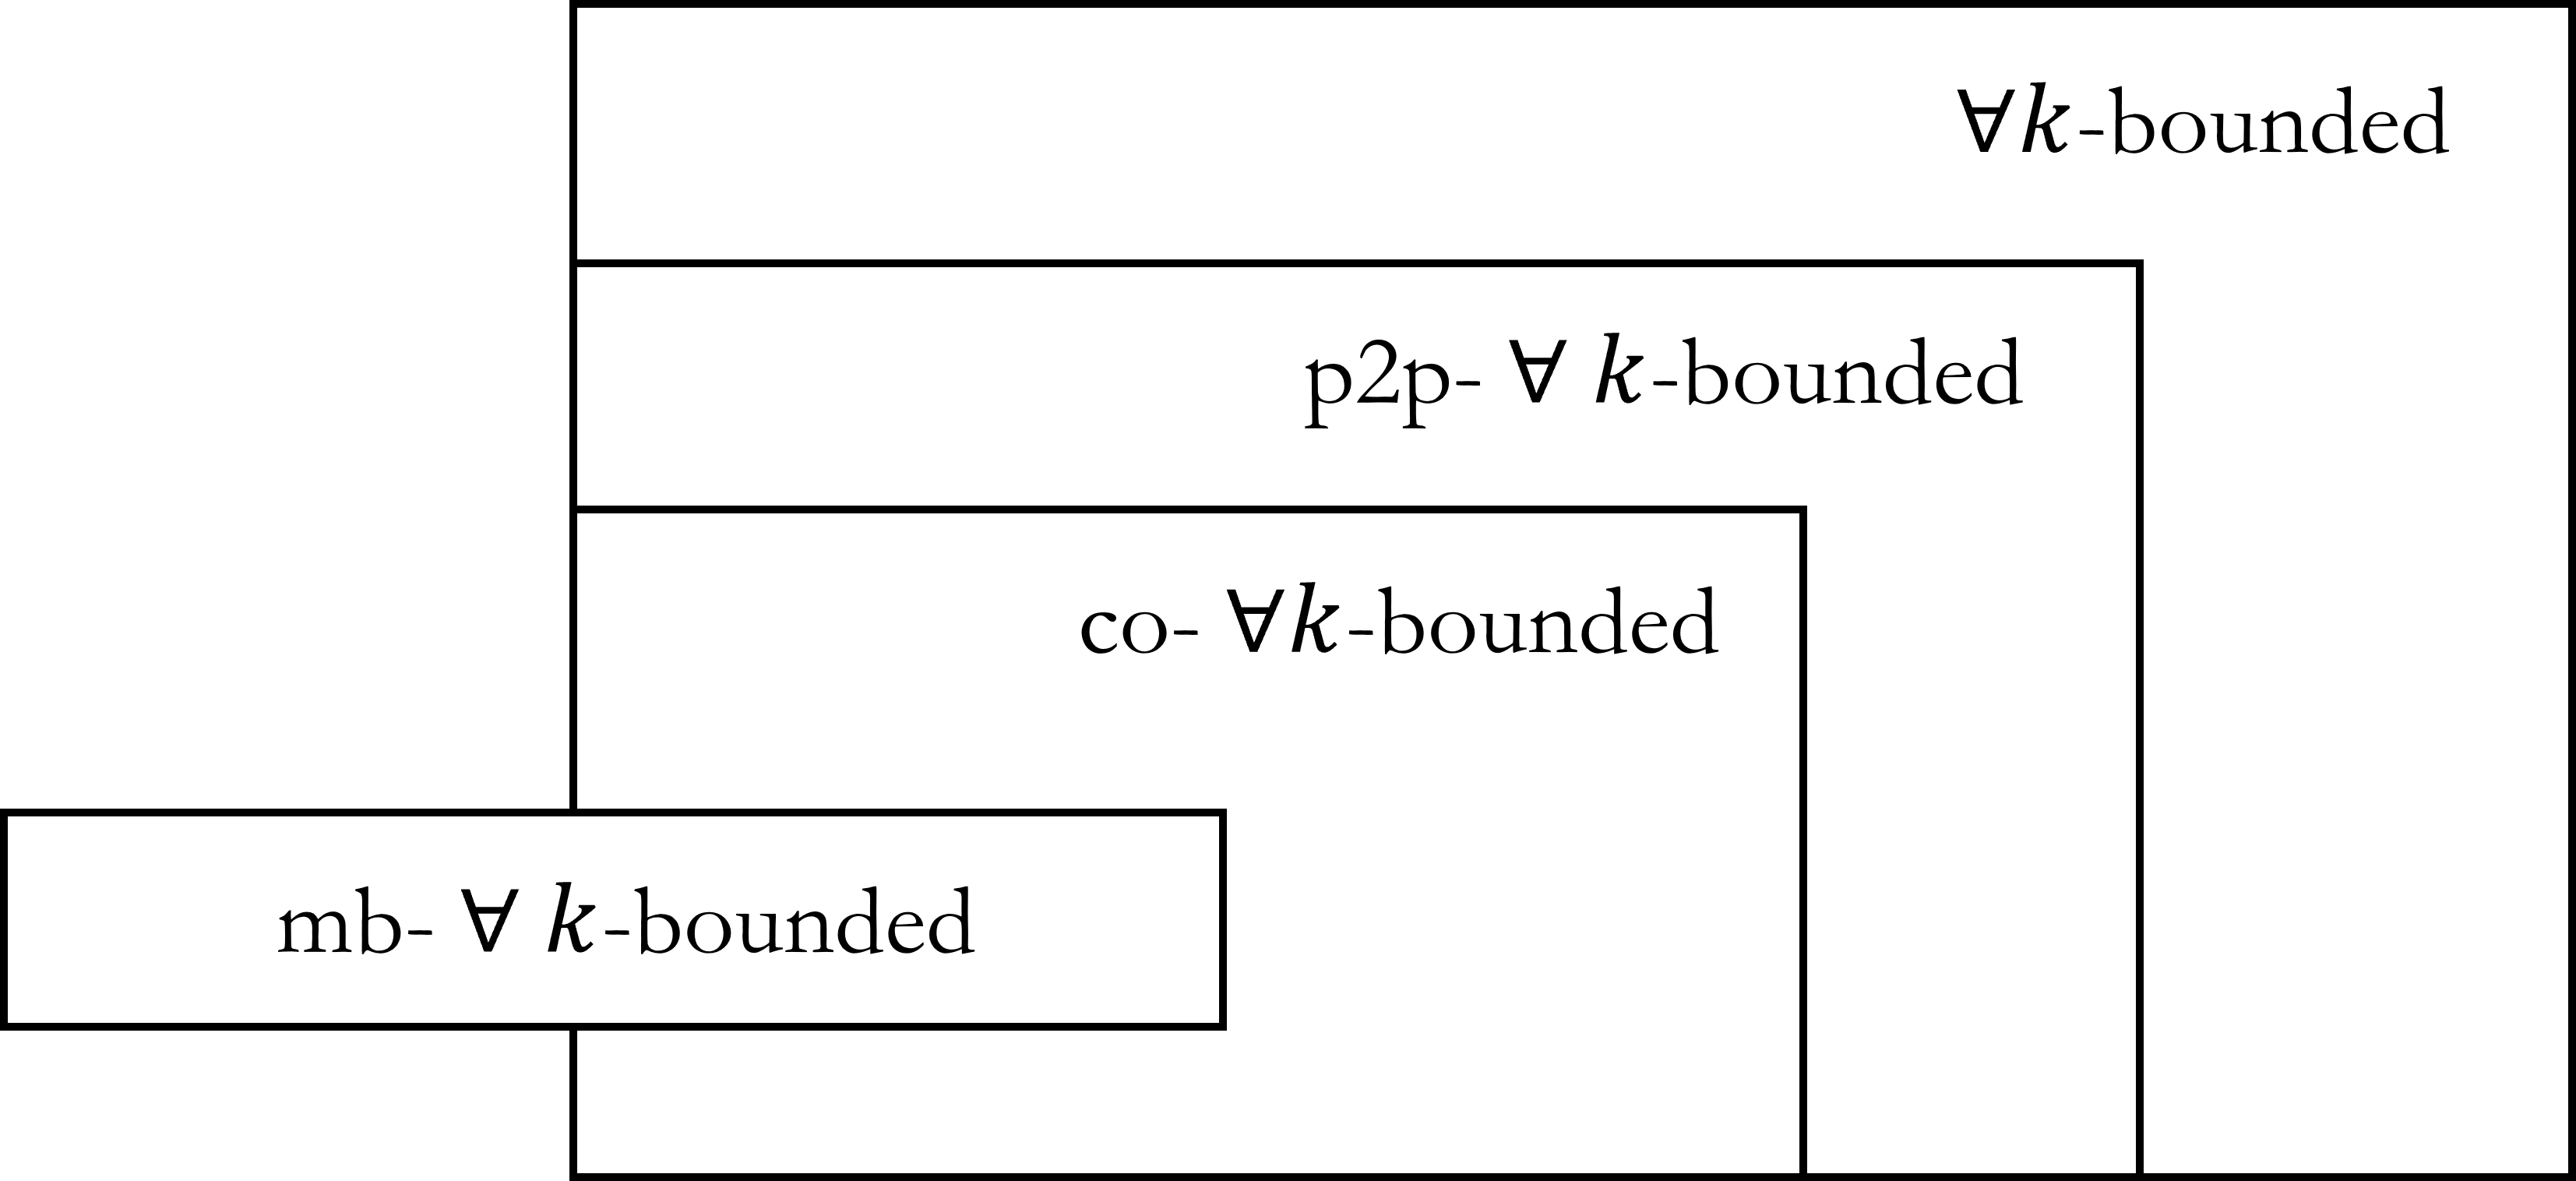
\includegraphics[width=8cm]{uni_k_hierarchy.png}
% 	\caption{The relation between different variants of universally $k$-bounded MSCs, given a $k \in \N$.}
% 	\label{fig:uk_hierarchy}
% \end{figure}

\paragraph*{MSO-definability}

In this section, we will investigate the MSO-definability of all the variants of universally $k$-bounded MSCs that we discussed.
In \cite{DBLP:conf/fossacs/LohreyM02}, it is shown that an MSC $\msc$ is universally $k$-bounded if and only if $\relb \;\subseteq\; \le$. In other words, $r \relb s \Rightarrow r \le s$ for any two events $r$ and $s$. This is equivalent to saying that every linearization $\linrel$ of $\msc$ respects the $\relb$ relation, since $\relb \;\subseteq\; \le \;\subseteq\; \linrel$. We already saw that $\relb$ is not MSO-definable when communication is asynchronous, hence we will use the $\relbAsy$ relation to give the following alternative characterization of universally $k$-bounded MSCs.

\begin{proposition}
	An MSC $\msc$ is $\forall k$-bounded if and only if $\relbAsy \;\subseteq\; \le$ and, for each channel ($p$,$q$), there are at most $k$ unmatched send events.
\end{proposition}
\begin{proof}
	($\Rightarrow$) Suppose $\msc$ is $\forall k$-bounded, which by definition means that all of its linearization are $k$-bounded. Firstly, notice that every MSC that has more than $k$ unmatched send events in any channel cannot be an $\forall k$-bounded MSC (not even $\exists k$-bounded). By contradiction, suppose that $\relbAsy \;\nsubseteq\; \le$, i.e. there are two events $r$ and $s$ such that $r \relbAsy s$ and $r \nleq s$. If $r \nleq s$, we either have that $s \le r$ or that $s$ and $r$ are incomparable w.r.t. $\le$; note that, in both cases, $\msc$ must have one linearization where $s$ happens before $r$\footnote{If two elements $a$ and $b$ of a set are incomparable w.r.t. a partial order $\le$, it is always possible to find a total order of the elements (that respects $\le$) where $a$ comes before $b$, or viceversa.}. The existence of such a linearization implies that $\msc$ is not $\forall k$-bounded.
	($\Leftarrow$) Suppose $\relbAsy \;\subseteq\; \le$ and, for each channel ($p$,$q$), there are at most $k$ unmatched send events. By definition, every linearization $\linrel$ of $\msc$ is such that $\le \;\subseteq\; \linrel$; it follows that $\relbAsy \;\subseteq\; \linrel$, which means that every linearization of $\msc$ is $k$-bounded, i.e. $\msc$ is $\forall k$-bounded.
\end{proof}

It follows that $\oneone$-$\forall k$-bounded and $\co$-$\forall k$-bounded MSCs are MSO-definable by definition, since $\oneone$ MSCs, causally ordered MSCs, and universally $k$-bounded MSCs are all MSO-definable. We already showed that $\relb$ is MSO-definable when considering $\oneone$ communication. The characterization for the other communication models is similar to that given in \cite{DBLP:conf/fossacs/LohreyM02}, but it uses the proper relation for each communication model.

\begin{proposition}\label{prop:mb_ukb_alt}
	An MSC $\msc$ is $\none$-$\forall k$-bounded if and only if $\relb \;\subseteq\; \mbpartial$.\\
	An MSC $\msc$ is onen-$\forall k$-bounded if and only if $\relb \;\subseteq\; \onenpartial$.\\
	An MSC $\msc$ is nn-$\forall k$-bounded if and only if $\relb \;\subseteq\; \bowtie$.
\end{proposition}
\begin{proof}
	We only show it for the $\none$ communication model. The proof for the other communication models works the same way. Consider an MSC $\msc$ and a $k \in \N$.\newline
	($\Leftarrow$) Suppose $\relb \;\subseteq\; \mbpartial$. For every mailbox linearization $\linrel$ of $\msc$ we have that $\mbpartial \;\subseteq\; \linrel$. This implies $\relb \;\subseteq\; \linrel$, that is to say every mailbox linearization is $k$-bounded.\newline
	($\Rightarrow$) Suppose $\msc$ is a $\none$-$\forall k$-bounded MSC. By definition, every mailbox linearization $\linrel$ of $\msc$ is $k$-bounded, i.e. $\relb \;\subseteq\; \linrel$, and we have $\mbpartial \;\subseteq\; \linrel$, according to the definition of mailbox linearization. Moreover, we also know that $\mbpartial \cup \relb$ is acyclic, since $\msc$ is $\exists k$-bounded\footnote{Every $\none$-$\forall k$-bounded MSC is also a $\none$-$\exists k$-bounded MSC by definition.}. Suppose now, by contradiction, that $\relb \;\nsubseteq\; \mbpartial$. Thus, there must be at least two events $r$ and $s$ such that $r \relb s$ and $r \npreceq s$; we also have $s \npreceq r$ because of the acyclicity of $\mbpartial \cup \relb$ (we cannot have the cycle $r \relb s \mbpartial r$). Consider a mailbox linearization $\linrel$  of $\msc$, such that $s \linrel r$. Note that such a mailbox linearization always exists, since $r$ and $s$ are incomparable w.r.t. the partial order $\mbpartial$. This mailbox linearization does not respect $\relb$ (because we have $s \linrel r$ and $r \relb s$), so it is not $k$-bounded. This is a contradiction, since we assumed that $\msc$ was a $\none$-$\forall k$-bounded MSC. It has to be that $\relb \;\subseteq\; \mbpartial$.
\end{proof}

Using Proposition~\ref{prop:mb_ukb_alt}, we can now easily write the MSO formulas that defines these variants of universally $k$-bounded MSCs.
\begin{align*}
	\mbUkformula &= \neg \exists r.\exists s.(r \relb s \wedge \neg(r \mbpartial s)) \\
	\onenUkformula &= \neg \exists r.\exists s.(r \relb s \wedge \neg(r \onenpartial s)) \\
	\nnUkformula &= \neg \exists r.\exists s.(r \relb s \wedge \neg(r \bowtie s))
\end{align*}


\paragraph*{Special treewidth}

All the variants of universally $k$-bounded MSCs that we presented have a bounded special treewidth. This directly follows from the STW-boundness of the existential counterparts, since every universally $k$-bounded MSC is existentially $k$-bounded by definition.


\section{Conclusion}\label{sec:conc}

%% Acknowledgments
\begin{acks}                            %% acks environment is optional
                                        %% contents suppressed with 'anonymous'
  %% Commands \grantsponsor{<sponsorID>}{<name>}{<url>} and
  %% \grantnum[<url>]{<sponsorID>}{<number>} should be used to
  %% acknowledge financial support and will be used by metadata
  %% extraction tools.
  This material is based upon work supported by the
  \grantsponsor{GS100000001}{National Science
    Foundation}{http://dx.doi.org/10.13039/100000001} under Grant
  No.~\grantnum{GS100000001}{nnnnnnn} and Grant
  No.~\grantnum{GS100000001}{mmmmmmm}.  Any opinions, findings, and
  conclusions or recommendations expressed in this material are those
  of the author and do not necessarily reflect the views of the
  National Science Foundation.
\end{acks}





% Bibliography
\bibliography{bibfile}
\newpage

\ifappendix

% %% Appendix
\appendix

\section{Additional material for Section~\ref{sec:MSO}}
\label{apx:MSO}
\cinzia{TODO: proofs mailbox alternative}
\cinzia{TODO: proofs 1-n alternative}
\subsection{MSO-definable properties}

In this sections we give MSO formulas for some MSO-definable properties that are used throughout the paper.

\paragraph*{Transitive Closure}
Given a binary relation $\to$, we can express its reflexive transitive closure $\to^*$ in MSO as
\[
x \to^* y = \forall X.(x \in X \;\wedge\; forward\_closed(X)) \implies y \in X
\]
\[
forward\_closed(X) = \forall z.\forall t.(z \in X \;\wedge\; z \to t) \implies t \in X
\]
The (non-reflexive) transitive closure of $\to$ can be simply expressed as
\[
x \to^+ y = x \to^* y \;\wedge\; x \neq y
\]

\paragraph*{Acyclicity} 

Given a binary relation $\to$, we can use MSO to express the acyclicity of $\to$. Recall that, given a binary relation $\to$, it is acyclic if and only if its transitive closure $\to^+$ is antisymmetric. The MSO formula of acyclicity directly follows from this definition:
\[
\Phi_{acyclic} =  \neg \exists x.(x \to^+ y \;\wedge\; y \to^+ x).   
\]
or, equivalently:
\[
\Phi_{acyclic} =  \neg \exists x.(x \to^+ x).   
\]

\subsection{Missing proofs}

\paragraph*{\bf Mailbox}

We show here that the two alternative definitions of $\none$ MSC that we gave are equivalent.

\begin{proposition}
    Definition~\ref{def:mb_msc} and Definition~\ref{def:n_one_alt} of $\none$ MSC are equivalent.
\end{proposition}
\begin{proof}
    ($\Rightarrow$)  We show that if $\msc$ is a $\none$ MSC, according to Definition~\ref{def:n_one_alt}, then it is also a $\none$ MSC, according to Definition~\ref{def:mb_msc}. By definition of $\mbpartial$, we must have 
    \begin{enumerate*}[label={(\roman*)}]
        \item $s \mbpartial s'$ for any two matched send events $s$ and $s'$ addressed to the same process, such that $r \procrel^+ r$, where $s \lhd r$ and $s' \lhd r'$, and
        \item $s \mbpartial s'$, if $s$ and $s'$ are a matched and an unmatched send event, respectively.
    \end{enumerate*} 
    If $\mbpartial$ is a partial order, we can find at least one linearization $\linrel$ such that $\mbpartial \;\subseteq\; \linrel$; such a linearization satisfies the conditions of Definition~\ref{def:mb_msc}.\newline
    ($\Leftarrow$) We show that if $\msc$ is not a $\none$ MSC, according to Definition~\ref{def:n_one_alt}, then it is also not a $\none$ MSC, according to Definition~\ref{def:mb_msc}. Since ${\mbpartial} = ({\procrel} \,\cup\, {\lhd} \,\cup\, {\mbrel})^\ast$ is not a partial order, $\mbpartial$ must be cyclic\footnote{$\mbpartial$ is reflexive and transitive by definition, if it were also acyclic it would be a partial order}. If $\mbpartial$ is cyclic, it means that we cannot find a linearization $\linrel$ such that $\mbpartial \;\subseteq\; \linrel$. In other words, we cannot find a linearization where      
    \begin{enumerate*}[label={(\roman*)}]
        \item $s \linrel s'$ for any two matched send events $s$ and $s'$ addressed to the same process, such that $r \procrel^+ r$, where $s \lhd r$ and $s' \lhd r'$, and
        \item $s \linrel s'$, if $s$ and $s'$ are a matched and an unmatched send event, respectively.
    \end{enumerate*} 
    It follows that $\msc$ is not a $\none$ MSC also according to Definition~\ref{def:mb_msc}.
\end{proof}

\paragraph*{\bf $\onen$}

We show here that the two alternative definitions of $\onen$ MSC that we gave are equivalent.

\begin{proposition}
    Definition~\ref{def:one_n} and Definition~\ref{def:one_n_alt} of $\onen$ MSC are equivalent.
\end{proposition}
\begin{proof}
    ($\Rightarrow$)  We show that if $\msc$ is a $\onen$ MSC, according to Definition~\ref{def:one_n_alt}, then it is also a $\onen$ MSC, according to Definition~\ref{def:one_n}. By definition of $\onenpartial$, we must have 
    \begin{enumerate*}[label={(\roman*)}]
        \item $r \onenpartial r'$ for any two receive events $r$ and $r'$ whose matched send events $s$ and $s'$ are such that $s \procrel^+ s'$, and
        \item $s \onenpartial s'$, if $s$ and $s'$ are a matched and an unmatched send event executed by the same process, respectively.
    \end{enumerate*} 
    If $\onenpartial$ is a partial order, we can find at least one linearization $\linrel$ such that $\onenpartial \;\subseteq\; \linrel$; such a linearization satisfies the conditions of Definition~\ref{def:one_n}.\newline
    ($\Leftarrow$) We show that if $\msc$ is not a $\onen$ MSC, according to Definition~\ref{def:one_n_alt}, then it is also not a $\onen$ MSC, according to Definition~\ref{def:one_n}. Since ${\onenpartial} = ({\procrel} \,\cup\, {\lhd} \,\cup\, {\onenrel})^\ast$ is not a partial order, $\onenpartial$ must be cyclic. If $\onenpartial$ is cyclic, it means that we cannot find a linearization $\linrel$ such that $\onenpartial \;\subseteq\; \linrel$. In other words, we cannot find a linearization where      
    \begin{enumerate*}[label={(\roman*)}]
        \item $r \linrel r'$ for any two receive events $r$ and $r'$ whose matched send events $s$ and $s'$ are such that $s \procrel^+ s'$, and
        \item $s \linrel s'$, if $s$ and $s'$ are a matched and an unmatched send event executed by the same process, respectively.
    \end{enumerate*} 
    It follows that $\msc$ is not a $\onen$ MSC also according to Definition~\ref{def:one_n}.
\end{proof}

\paragraph*{\bf $\nn$}

We show here the missing proofs for the equivalence of the two definitions of $\nn$ MSC that we gave.

\nnfirstprop*
\begin{proof}
    Follows from the definition of $\nnbowtie$. We have $r_1 \nnbowtie r_2$ if either:
    \begin{itemize}%\itemsep=0.5ex
        \item $r_1 \nnrel r_2$. Two cases: either \begin{enumerate*}[label={(\roman*)}]
            \item $s_1 \nnrel s_2$, or 
            \item $s_1 \slashed{\nnrel} s_2$.
        \end{enumerate*}
        The first case clearly implies $s_1 \nnbowtie s_2$, for rule 1 in the definition of $\nnbowtie$. The second too, because of rule 3.
        \item  $r_1 \slashed{\nnrel} r_2$, but $r_1 \nnbowtie r_2$. This is only possible if rule 2 in the definition of $\nnbowtie$ was used, which implies $s_1 \nnrel s_2$ and, for rule 1, $s_1 \nnbowtie s_2$.
    \end{itemize}
\end{proof}

\nnsecondprop*
\begin{proof}
    According to Definition~\ref{def:n_n}, an MSC is $\nn$ if it has at least one $\nn$ linearization. Note that, because of how it is defined, any $\nn$ linearization is always both a $\none$ and a $\onen$ linearization. It follows that the cyclicity of $\nnrel$ (not $\nnbowtie$) implies that $\msc$ is not $\nn$, because it means that we are not even able to find a linearization that is both $\none$ and $\onen$. Moreover, since in a $\nn$ linearization the order in which messages are sent matches the order in which they are received, and unmatched send events can be executed only after matched send events, a $\nn$ MSC always has to satisfy the constraints imposed by the $\nnbowtie$ relation. If $\nnbowtie$ is cyclic, then for sure there is no $\nn$ linearization for $\msc$.
    \davide{This proof is not very formal... do you think it is fine?}
\end{proof}    

\nnalgotermination*
\begin{proof}
We want to prove that, if $\nnbowtie$ is acyclic, step 4 of the algorithm is never executed, i.e. it terminates correctly. Note that the acyclicity of $\nnbowtie$ implies that the EDG of $\msc$ is a DAG. Moreover, at every step of the algorithm we remove nodes and edges from the EDG, so it still remains a DAG. The proof goes by induction on the number of events added to the linearization.\newline
Base case: no event has been added to the linearization yet. Since the EDG is a DAG, there must be an event with in-degree 0. In particular, this has to be a send event (a receive event depends on its respective send event, so it cannot have in-degree 0). If it is a matched send event, step 1 is applied. If there are no matched send events, step 2 is applied on an unmatched send. We show that it is impossible to have an unmatched send event of in-degree 0 if there are still matched send events in the EDG, so either step 1 or 2 are applied in the base case. Let $s$ be one of those matched send events and let $u$ be an unmatched send. Because of rule 4 in the definition of $\nnbowtie$, we have that $s \nnbowtie u$, which implies that $u$ cannot have in-degree 0 if $s$ is still in the EDG.\newline
Inductive step: we want to show that we are never going to execute step 4. In particular, Step 4 is executed when none of the first three steps can be applied. This happens when there are no matched send events with in-degree 0 and one of the following holds:
\begin{itemize}%\itemsep=0.5ex
	\item \emph{There are still matched send events in the EDG with in-degree $>0$, there are no unmatched messages with in-degree 0, and there is no receive event $r$ with in-degree 0 in the EDG, such that $r$ is the receive event of the first message whose sent event was already added to the linearization}. Since the EDG is a DAG, there must be at least one receive event with in-degree 0. We want to show that, between these receive events with in-degree 0, there is also the receive event $r$ of the first message whose send event was added to the linearization, so that we can apply step 3 and step 4 is not executed. Suppose, by contradiction, that $r$ has in-degree $>0$, so it depends on other events. For any maximal chain in the EDG that contains one of these events, consider the first event $e$, which clearly has in-degree 0. In particular, $e$ cannot be a send event, because we would have applied step 1 or step 2. Hence, $e$ can only be a receive event for a send event that was not the first added to the linearization (and whose respective receive still has not been added). However, this is also impossible, since $r_e \nnbowtie r$ implies $s_e \nnbowtie s$, and we could not have added $s$ to the linearization before $s_e$. Because we got to a contradiction, the hypothesis that $r$ has in-degree $>0$ must be false, and we can indeed apply step 3.
	\item \emph{There are still matched send events in the EDG with in-degree $>0$, there is at least one unmatched message with in-degree 0, and there is no receive event $r$ with in-degree 0 in the EDG, such that $r$ is the receive event of the first message whose sent event was already added to the linearization}. We show that it is impossible to have an unmatched send event of in-degree 0 if there are still matched send events in the EDG. Let $s$ be one of those matched send events and let $u$ be an unmatched send. Because of rule 4 in the definition of $\nnbowtie$, we have that $s \nnbowtie u$, which implies that $u$ cannot have in-degree 0 if $s$ is still in the EDG.
	\item \emph{There are no more matched send events in the EDG, there are no unmatched messages with in-degree 0, and there is no receive event $r$ with in-degree 0 in the EDG, such that $r$ is the receive event of the first message whose sent event was already added to the linearization}. Very similar to the first case. Since the EDG is a DAG, there must be at least one receive event with in-degree 0. We want to show that, between these receive events with in-degree 0, there is also the receive event $r$ of the first message whose send event was added to the linearization, so that we can apply step 3 and step 4 is not executed. Suppose, by contradiction, that $r$ has in-degree $>0$, so it depends on other events. For any maximal chain in the EDG that contains one of these events, consider the first event $e$, which clearly has in-degree 0. In particular, $e$ cannot be a send event, because by hypothesis there are no more send events with in-degree 0 in the EDG. Hence, $e$ can only be a receive event for a send event that was not the first added to the linearization (and whose respective receive still has not been added). However, this is also impossible, since $r_e \nnbowtie r$ implies $s_e \nnbowtie s$, and we could not have added $s$ to the linearization before $s_e$. Because we got to a contradiction, the hypothesis that $r$ has in-degree $>0$ must be false, and we can indeed apply step 3.
\end{itemize}
We showed that, if $\nnbowtie$ is acyclic, the algorithm always terminates correctly and computes a valid $\nn$ linearization.
\end{proof}


\section{Additional material for Section~\ref{sec:hierarchy}}
\label{apx:hierarchy}
\begin{proposition} \label{prop:co_is_pp}
	Every $\co$ MSC is a $\oneone$ MSC.
\end{proposition}
\begin{proof}
	According to Definition~\ref{def:co_msc}, and MSC is $\co$ if, for any two send events $s$ and $s'$, such that $\lambda(s)=\pqsAct{\plh}{q}$, $\lambda(s')=\pqsAct{\plh}{q}$, and $s \le s'$, we have either
	\begin{enumerate*}[label={(\roman*)}]
		\item $s,s' \in \Matched{\msc}$ and $r \procrel^* r'$, where $r$ and $r'$ are two receive events such that $s \lhd r$ and $s' \lhd r'$, or
		\item $s' \in \Unm{\msc}$.
	\end{enumerate*}
	The conditions imposed by the Definition~\ref{def:pp_msc} of $\oneone$ are clearly satified by any causally ordered MSC; in particular, note that $s \procrel^+ s'$ implies $s \le s'$.
\end{proof}

\mbonennounmatched*
\begin{proof}
	We show that the contrapositive is true, i.e. if an MSC is not $\onen$ (and it does not have unmatched messages), it is also not mailbox. Suppose $\msc$ is an asynchronous MSC, but not $\onen$. There must be a cycle $\xi$ such that  $e \onenpartial e$, for some event $e$. Recall that ${\onenpartial} = ({\procrel} \,\cup\, {\onenrel} \,\cup\, {\mbrel})^\ast$ and ${\le} = ({\procrel} \cup {\onenrel})^\ast$. We can always explicitely write a cycle $e \onenpartial e$ only using $\onenrel$ and $\le$. For instance, there might be a cycle $e \onenpartial e$ because we have that $e \onenrel f \le g \onenrel h \onenrel i \le e$. Consider any two adiacent events $r_1$ and $r_2$ in the cycle $\xi$, where $\xi$ has been written using only $\onenrel$ and $\le$, and we never have two consecutive $\le$. We have two cases:
	\begin{enumerate}
		\item $r_1 \onenrel r_2$. By definition of $\onenrel$, $r_1$ and $r_2$ must be two receive events, since we are not considering unmatched send events, and $s_1 \procrel^+ s_2$, where $s_1$ and $s_2$ are the send events that match with $r_1$ and $r_2$, respectively.
		\item $r_1 \le r_2$. Since $\msc$ is asynchronous by hyphotesis, $\xi$ has to contain at least one $\onenrel$; recall that we also wrote $\xi$ in such a way that we do not have two consecutive $\le$. It is not difficult to see that $r_1$ and $r_2$ have to be receive events, since they belong to $\xi$. Let $s_1$ and $s_2$ be the two send events such that $s_1 \lhd r_1$ and $s_2 \lhd r_2$. We have two cases:
		\begin{enumerate}
			\item $s_2$ is in the causal path between $r_1$ and $r_2$, i.e. $s_1 \lhd r_1 \le s_2 \lhd r_2$. In particular, note that $s_1 \le s_2$.
			\item $s_2$ is not in the causal path between $r_1$ and $r_2$, hence there must be a message $m_k$ received by the same process that executes $r_2$, such that $r_1 \le s_k \lhd r_k \procrel^+ r_2$, where $r_k$ is the send event of $m_k$. Since messages $m_k$ and $m_2$ are received by the same process and $r_k \procrel^+ r_2$, we should have $s_k \mbrel s_2$, according to the mailbox semantics. In particular, note the we have $s_1 \le s_k \mbrel s_2$.
		\end{enumerate}
		In both case (a) and (b), we conclude that $s_1 \mbpartial s_2$. Recall that ${\mbpartial} = ({\procrel} \,\cup\, {\lhd} \,\cup\, {\mbrel})^\ast$.
	\end{enumerate}
	Notice that, for either cases, a relation between two receive events $r_1$ and $r_2$ implies a relation between the respective send events $s_1$ and $s_2$, according to the mailbox semantics. It follows that $\xi$, which is a cycle for the $\onenpartial$ relation, always implies a cycle for the $\mbpartial$ relation.
	\end{proof}

	\begin{proposition} \label{prop:nn_is_onen}
		Every $\nn$ MSC is a $\onen$ MSC.
	\end{proposition}
	\begin{proof}
		Consider Definition~\ref{def:n_n} and Definition~\ref{def:one_n}. They are identical, except for the fact that in the $\nn$ case we consider any two send events, and not just those that are sent by a same process. This is enough to show that each $\nn$ linearization is also a $\onen$ linearization and, therefore, each $\nn$ MSC is a $\onen$ MSC.
	\end{proof}
	
	\begin{proposition} \label{prop:rsc_is_nn}
		Every $\rsc$ MSC is a $\nn$ MSC.
	\end{proposition}
	\begin{proof}
		Consider Definition~\ref{def:rsc} and Definition~\ref{def:n_n}. Let us pick an $\rsc$ linearization $\linrel$. If every send event is immediately followed by its matching receive event, and we do not have unmatched messages, then $\linrel$ is also a $\nn$ linearization; note that, for any two send events $s$ and $s'$ such that $s \linrel s'$, we also have $r \linrel r'$, where $s \lhd r$ and $s' \lhd r'$. It follows that each $\rsc$ MSC is a $\nn$ MSC.
	\end{proof}
	

\section{Additional material for Section~\ref{sec:checking}}
\label{apx:checking}
\subsection{Communicating finite state machines\label{app:cfsm}}
We now recall the definition of communicating systems (aka communicating finite-state
machines or message-passing automata), which consist of finite-state machines $A_p$
(one for every process $p \in \Procs$) that can communicate through channels from $\Ch$.

\begin{definition}\label{def:cs}
A \emph{system of communicating finite state machines} over the set $\Procs$ of rocesses
and the set $\Msg$ of messages is a tuple
   $ \Sys = (A_p)_{p\in\procSet}$. For each
   $p \in \Procs$, $A_p = (Loc_p, \delta_p, \ell^0_p)$ is a finite transition system where
   $\Loc_p$ is a finite set of local (control) states, $\delta_p
   \subseteq \Loc_p \times \pAct{p} \times \Loc_p$ is the
   transition relation, and $\ell^0_p \in Loc_p$ is the initial state.
\end{definition}

Given $p \in \Procs$ and a transition $t = (\ell,a,\ell') \in \delta_p$, we let
$\tsource(t) = \ell$, $\ttarget(t) = \ell'$, $\tlabel(t) = a$, and
$\tmessage(t) = \msg$ if $a \in \msAct{\msg} \cup \mrAct{\msg}$.

% \smallskip

% There are in general two ways to define the semantics of a communicating system.
% Most often it is defined as a global infinite transition system that keeps track
% of the various local control states and all (unbounded) channel contents.
% As, in this paper, our arguments are based on a graph view of MSCs, we will define
% the language of $\Sys$ directly as a set of MSCs. These two semantic views are essentially
% equivalent, but they have different advantages depending on the context.
% We refer to \cite{CyriacG14} for a thorough discussion.

% \davidequestion{MSCs are formally defined in chapter 5... maybe move here in the preliminaries just the asynchronous definition?}

Let $\msc = (\Events,\procrel,\lhd,\lambda)$ be an MSC.
A \emph{run} of $\Sys$ on $\msc$ is a mapping
$\rho: \Events \to \bigcup_{p \in \Procs} \delta_p$
that assigns to every event $e$ the transition $\rho(e)$
that is executed at $e$. Thus, we require that
\begin{enumerate*}[label={(\roman*)}]
\item for all $e \in \Events$, we have $\tlabel(\rho(e)) = \lambda(e)$,
\item for all $(e,f) \in {\procrel}$, $\ttarget(\rho(e)) = \tsource(\rho(f))$,
\item for all $(e,f) \in {\lhd}$, $\tmessage(\rho(e)) = \tmessage(\rho(f))$,
and
\item for all $p \in \Procs$ and $e \in \Events_p$ such that there is no $f \in \Events$ with $f \procrel e$, we have $\tsource(\rho(e)) = \ell_p^0$.
\end{enumerate*}

We write $L_{\asy}(\Sys)$ to denote the set of MSCs $\msc$ that admit a run of $\Sys$.
Intuitively, $L_{\asy}(\Sys)$ is the set of all asynchronous behaviors of $\Sys$.

% Letting run $\Sys$ directly on MSCs is actually very convenient.
% This allows us to associate with $\Sys$ its p2p language and mailbox language
% in one go. The \emph{\pp language} of $\Sys$ is $\ppL{\Sys} = \{\msc \in \ppMSCs \mid$ there is a run of $\Sys$ on $\msc\}$.
% The \emph{mailbox language} of $\Sys$ is $\mbL{\Sys} = \{\msc \in \mbMSCs \mid$ there is a run of $\Sys$ on $\msc\}$.
%
% Note that, following \cite{DBLP:conf/cav/BouajjaniEJQ18,DBLP:conf/fossacs/GiustoLL20},
% we do not consider final states or final configurations, as our purpose is to
% reason about all possible
% traces that can be \emph{generated} by $\Sys$.
% %We will discuss this issue in more detail later in the paper. \todo{Do we still discuss this in the conference version or can we omit this sentence?}

\subsection{Conflict Graph}\label{app:conflict-graph}

%\etienne{Copy-paste from a file, not sure how it fits with the rest of the appendix yet.}
%\davidequestion{The conflict graph is needed only for some proofs on the cuncur paper. I think it makes sense not to include it here and eventually introduce it later in the MSO-treewidth chapter if we really need it.}

We now recall the notion of a conflict graph associated to an MSC defined in \cite{DBLP:conf/cav/BouajjaniEJQ18}. This graph is used to depict the causal dependencies between message exchanges.  Intuitively, we have a dependency whenever
two messages have a process in common. For instance, an $\xrightarrow{SS}$
dependency between message exchanges $v$ and $v'$ expresses the fact that
$v'$ has been sent after $v$, by the same process. This notion is of interest because it was seen in \cite{DBLP:conf/cav/BouajjaniEJQ18} that the notion of synchronizability in MSCs (which is studied in this paper) can be graphically characterised by the nature of the associated conflict graph.
It is defined in terms of linearizations
in \cite{DBLP:conf/fossacs/GiustoLL20}, but we equivalently express it
directly in terms of MSCs.

For an MSC $\msc = (\Events, \rightarrow, \lhd, \lambda)$ and
$e \in \Events$, we define the type $\type(e) \in \{\stype,\rtype\}$ of $e$ by $\type(e) = \stype$ if $e \in \SendEv{\msc}$
and $\type(e) = \rtype$ if $e \in \RecEv{\msc}$.
Moreover, for $e \in \Unm{\msc}$, we let $\mexch(e) = e$,
and for $(e,e') \in \lhd$, we let $\mexch(e) = \mexch(e') = (e,e')$.


\begin{definition}[Conflict graph]
	The \emph{conflict graph} $\cgraph{\msc}$ of an MSC $\msc = (\Events, \rightarrow, \lhd, \lambda)$ is the labeled graph $(\Nodes, \Edges)$, with $\Edges \subseteq \Nodes \times \{\stype,\rtype\}^2 \times \Nodes$, defined by
	$\Nodes = {\lhd} \cup \Unm{\msc}$ and $\Edges = \{(\mu(e),\type(e)\type(f),\mu(f)) \mid (e,f) \in {\to^+}\}$.
In particular, a node of $\cgraph{\msc}$ is either a single unmatched send event or a message pair $(e,e') \in {\lhd}$.
\end{definition}


\subsection{Proof of Theorem~\ref{thm:bounded-model-checking}}\label{proofbmc}


\thmBoundedMC*

\begin{proof}
   Let $\comsymb$, $\aMSCclass$, $\Sys$, and $\amsoformula$ 
   be fixed. We showed in Section~\ref{sec:MSO} 
   that there is a MSO formula
   $\msoformulaofcom{\comsymb}$
   that defines $\MSCclassofcom{\comsymb}$.
   There is also a MSO formula
   $\amsoformula_{\Sys}$ such that
   $L_{\asy}(\Sys)=L(\amsoformula_{\Sys})$.\footnote{The formula
   simply encodes the existence of a run of $\Sys$ on the MSC
   using a MSO variable $X_l$ for each control
   state $l$, with the meaning that $X_l$ is the set of events
   before which the local communicating automaton was in state $l$. See \cite[Theorem~3.4]{DBLP:journals/corr/abs-1904-06942} for a detailed proof.}
   Putting everything together, we have
    \[\begin{array}{rl}
    &L_{\comsymb}(\System) \cap \stwMSCs{k} \subseteq L(\amsoformula)\\[1ex]
    \Longleftrightarrow &\asyL{\System} \cap \MSCclassofcom{\comsymb} \cap \stwMSCs{k} \subseteq L(\phi)\\[1ex]
    \Longleftrightarrow & L(\amsoformula_{\System}) \cap L(\msoformulaofcom{\comsymb}) \cap \stwMSCs{k} \subseteq L(\phi)\\[1ex]
    \Longleftrightarrow &\stwMSCs{k} \subseteq L(\phi \vee \neg \msoformulaofcom{\comsymb}\vee\neg\amsoformula_{\System})\,.
    \end{array}\]

    The latter is decidable by Courcelle's theorem~\cite{Courcelle10}.
\end{proof}


\subsection{Proof of Theorem~\ref{thm:sync}}
\label{apx:sync}
In order to prove Theorem \ref{thm:sync}, we first need to introduce some concepts and give preliminary proofs. 

\begin{definition}[Prefix]
	Let $\msc = (\Events,\procrel,\lhd,\lambda) \in \MSCs$ and consider
	$E \subseteq \Events$ such that $E$ is ${\le}$-\emph{downward-closed}, i.e,
	for all $(e,f) \in {\le}$ such that $f \in E$, we also have $e \in E$.
	Then, the MSC $M' = (E,{\procrel} \cap (E \times E),{\lhd} \cap (E \times E),\lambda')$,
	where $\lambda'$ is the restriction of $\Events$ to $E$, is called a \emph{prefix}
	of $\msc$. 	
\end{definition}

If we consider a set $E$ that is ${\onenpartial}$-\emph{downward-closed}, we call $M'$ a \emph{$\onen$ prefix}.
If the set $E$ is ${\bowtie}$-\emph{downward-closed}, we call $M'$ a \emph{$\nn$ prefix}. Note that every $\onen$ or $\nn$ prefix is also a prefix, since $\le \subseteq {\onenpartial}$ and $\le \subseteq {\bowtie}$.

Note that the empty MSC is a prefix of $\msc$.
We denote the set of prefixes of $\msc$ by $\Pref{\msc}$, whereas $\Prefonen{\msc}$ and $\Prefnn{\msc}$ are used for the $\onen$ and the $\nn$ variants, respectively.
This is extended to sets $L \subseteq \MSCs$ as expected, letting
$\Pref{L} = \bigcup_{\msc \in L} \Pref{\msc}$.

\begin{proposition}
	\label{prop:prefixes}
	For $\comsymb \in \{\asy, \oneone, \co, \none\}$, every prefix of a $\comsymb$ MSC is a $\comsymb$ MSC.
\end{proposition}
\begin{proof}
    For $\comsymb = \asy$ it is true by definition. For $\comsymb = \{\oneone, \none\}$ it was already shown to be true in \cite{BolligFG21}, so we just consider $\comsymb = \co$. Let $\msc = (\Events, \procrel, \lhd, \lambda) \in \coMSCs$ and let $\msc_0 =
    (\Events_0, \procrel_0, \lhd_0, \lambda_0)$ be a prefix of $\msc$. By contradiction, suppose that $\msc_0$ is not a	causally ordered MSC. There must be two distinct $s,s' \in \Events_0$ such that $\lambda(s)=\pqsAct{\plh}{q}$, $\lambda(s')=\pqsAct{\plh}{q}$, $s \le_{\msc_0} s'$ and either
    \begin{enumerate*}[label={(\roman*)}]
        \item $r' \procrel^+ r$, where $r$ and $r'$ are two receive events such that $s \lhd r$ and $s' \lhd r'$, or
        \item $s \in \Unm{\msc_0}$ and $s' \in \Matched{\msc_0}$.
    \end{enumerate*}
    In both cases, $\msc$ would also not be a causally ordered $\MSCs$, since $\Events_0 \subseteq \Events$, ${\rightarrow_0} \subseteq {\rightarrow}$, and ${\lhd_0} \subseteq {\lhd}$. This is a contradiction, thus $\msc_0$ has to be causally ordered.
\end{proof}

Note that this proposition is not true for the $\onen$ and the $\nn$ communication models. Fig.\ref{fig:onen-prefix} shows an example of $\nn$ MSC with a prefix that is neither a $\nn$ MSC nor a $\onen$ MSC.

\begin{figure}[t]
	\captionsetup[subfigure]{justification=centering}
% \centering
\begin{subfigure}[t]{0.45\textwidth}\centering
	\begin{tikzpicture}[scale=0.7, every node/.style={transform shape}]
		\newproc{0}{p}{-1.5};
		\newproc{1}{q}{-1.5};
		\newproc{2}{r}{-1.5};

		\newmsgm{0}{1}{-0.5}{-0.5}{1}{0.3}{black};
		\newmsgm{0}{2}{-1.0}{-1.0}{2}{0.7}{black};

	\end{tikzpicture}
	\caption{A $\nn$ MSC $\msc$.}
\end{subfigure}
% \hfill
\begin{subfigure}[t]{0.45\textwidth}\centering
	\begin{tikzpicture}[scale=0.7, every node/.style={transform shape}]
		\newproc{0}{p}{-1.5};
		\newproc{1}{q}{-1.5};
		\newproc{2}{r}{-1.5};

		\newmsgum{0}{1}{-0.5}{1}{0.3}{black};
		\newmsgm{0}{2}{-1.0}{-1.0}{2}{0.7}{black};

	\end{tikzpicture}
	\caption{A prefix of $\msc$.}
\end{subfigure}
	\caption{A $\nn$ MSC with a prefix that is neither $\onen$ nor $\nn$.}
	\label{fig:onen-prefix}
\end{figure}

\begin{proposition}
	\label{prop:prefixes-onen}
	Every $\onen$ prefix of a $\onen$ MSC is a $\onen$ MSC.
\end{proposition}
\begin{proof}
    Let $\msc = (\Events, \procrel, \lhd, \lambda) \in \onenMSCs$ and let $\msc_0 =
    (\Events_0, \procrel_0, \lhd_0, \lambda_0)$ be a $\onen$ prefix of $\msc$, where $\Events_0 \subseteq \Events$. Firstly, the $\onenpartial$-downward-closeness of $\Events_0$ guarantees that ${\msc_0}$ is still an MSC. We need to prove that it is a $\onen$ MSC. By contradiction, suppose that $\msc_0$ is not a $\onen$ MSC. Then, there are distinct $e,f \in \Events_0$ such that $e \onenpartial_{\msc_0} f \onenpartial_{\msc_0} e$, where $\onenpartial_{\msc_0} = (\procrel_0 \cup \lhd_0 \cup \onenrel_{\msc_0})^\ast$. As $\Events_0 \subseteq \Events$, we have that ${\rightarrow_0} \subseteq {\rightarrow}$, ${\lhd_0} \subseteq {\lhd}$, ${\onenrel_{\msc_0}} \subseteq {\onenrel}$. Clearly, $\onenpartial_{\msc_0} \subseteq \onenpartial$, so $e \onenpartial f \onenpartial e$. This implies that $\msc$ is not a $\onen$ MSC, because $\onenpartial$ is cyclic, which is a contradiction. Hence $\msc_0$ is a $\onen$ MSC.
\end{proof}

\begin{proposition}
	\label{prop:prefixes-nn}
	Every $\nn$ prefix of a $\nn$ MSC is a $\nn$ MSC.
\end{proposition}
\begin{proof}
	Let $\msc = (\Events, \procrel, \lhd, \lambda) \in \nnMSCs$ and let $\msc_0 =
	(\Events_0, \procrel_0, \lhd_0, \lambda_0)$ be a $\nn$ prefix of $\msc$, where $\Events_0 \subseteq \Events$. Firstly, the $\bowtie_\msc$-downward-closeness of $\Events_0$ guarantees that ${\msc_0}$ is still an MSC. We need to prove that it is a $\nn$ MSC. By contradiction, suppose that $\msc_0$ is not a $\nn$ MSC. Then, there are distinct $e,f \in \Events_0$ such that $e \bowtie_{\msc_0} f \bowtie_{\msc_0} e$. As $\Events_0 \subseteq \Events$, we have that ${\rightarrow_0} \subseteq {\rightarrow}$, ${\lhd_0} \subseteq {\lhd}$, ${\nnrel_0} \subseteq {\nnrel}$. Clearly, $\bowtie_{\msc_0} \subseteq\; \bowtie_\msc$, so $e \bowtie_\msc f \bowtie_\msc e$. This implies that $\msc$ is not a $\nn$ MSC, because $\bowtie_\msc$ is cyclic, which is a contradiction. Hence $\msc_0$ is a $\nn$ MSC.
\end{proof}

The next lemma is about the prefix closure of a communicating system and it follows from Proposition \ref{prop:prefixes}.

\begin{proposition}\label{lem:co-prefix-closed}
	For all $\comsymb \in \{\asy, \ppsymb, \mbsymb, \cosymb\}$, $\cL{\Sys}$ is prefix-closed:
	$\Pref{\cL{\Sys}} \subseteq \cL{\Sys}$.
\end{proposition}

Similar results also hold for the $\onen$ and $\nn$ communication models.

\begin{proposition}\label{lem:onen-prefix-closed}
	$\onenL{\Sys}$ is $\onen$ prefix-closed:
	$\Prefonen{\onenL{\Sys}} \subseteq \onenL{\Sys}$.
\end{proposition}
\begin{proof}
	Given a system $\System$, we have that $\onenL{\System} = \ppL{\System} \cap \onenMSCs$. Note that, because of how we defined a $\onen$ prefix, we have that $\Prefonen{\onenL{\Sys}} = \Pref{\onenL{\Sys}} \cap \onenMSCs$. Moreover, $\Pref{\onenL{\Sys}} \subseteq \Pref{\ppL{\Sys}}$, and $\Pref{\onenL{\Sys}} \subseteq \ppL{\Sys}$ for Proposition~\ref{lem:prefix-closed}. Putting everything together, $\Prefonen{\onenL{\Sys}} \subseteq \ppL{\Sys} \cap \onenMSCs = \onenL{\System}$.
\end{proof}

\begin{proposition}\label{lem:nn-prefix-closed}
	$\nnL{\Sys}$ is $\nn$ prefix-closed:
	$\Prefnn{\nnL{\Sys}} \subseteq \nnL{\Sys}$.
\end{proposition}
\begin{proof}
	Given a system $\System$, we have that $\nnL{\System} = \ppL{\System} \cap \nnMSCs$. Note that, because of how we defined a $\nn$ prefix, we have that $\Prefnn{\nnL{\Sys}} = \Pref{\nnL{\Sys}} \cap \nnMSCs$. Moreover, $\Pref{\nnL{\Sys}} \subseteq \Pref{\ppL{\Sys}}$, and $\Pref{\nnL{\Sys}} \subseteq \ppL{\Sys}$ for Proposition~\ref{lem:prefix-closed}. Putting everything together, $\Prefnn{\nnL{\Sys}} \subseteq \ppL{\Sys} \cap \nnMSCs = \nnL{\System}$.
\end{proof}

In general, even simple verification problems, such
as control-state reachability, are undecidable for
communicating systems \cite{DBLP:journals/jacm/BrandZ83}.
However, they are decidable when we restrict to behaviors of
bounded special tree-width, which motivates the following
definition of a generic \emph{bounded model-checking} problem for $\{\asy, \oneone, \co, \none, \onen, \nn \}$ :\\
%
{\bf Input:} Two finite sets $\Procs$ and $\Msg$, a communicating system $\System$, an MSO sentence $\phi$, and $k \in \N$.\\
%
{\bf Question:} Do we have $\cL{\Sys} \cap \stwMSCs{k} \subseteq L(\phi)$?

\begin{theorem}
	\label{thm:bounded_model_checking}
	The bounded model-checking problem for $\comsymb \in \{$$\asy, $ $\oneone, $ $\co, $ $\none, $ $\onen, $ $\nn\}$ is decidable.
\end{theorem}
\davidequestion{Proof missing for $\asy$, Courcelle's theorem?}

\begin{proof}
    For $\comsymb = \{\oneone, \none\}$ refer to \cite{BolligFG21}. 
    Consider $\comsymb = \co$. As shown in Section~\ref{sec:MSO}, $\coMSCs=L(\coformula)$. Given a system $\System$, we then have that $\coL{\System} = \ppL{\System} \cap L(\coformula)$. We can rewrite the bounded model-checking problem for $\comsymb = \cosymb$ as
    \[\begin{array}{rl}
    &\coL{\System} \cap \stwMSCs{k} \subseteq L(\phi)\\[1ex]
    \Longleftrightarrow &\ppL{\System} \cap L(\coformula) \cap \stwMSCs{k} \subseteq L(\phi)\\[1ex]
    \Longleftrightarrow &\ppL{\System} \cap \stwMSCs{k} \subseteq L(\phi) \cup L(\neg \coformula)\\[1ex]
    \Longleftrightarrow &\ppL{\System} \cap \stwMSCs{k} \subseteq L(\phi \vee \neg \coformula)\,.
    \end{array}\]

    The latter is an instance of the bounded model-checking problem for the $\oneone$ communication model, which was already shown to be decidable. The technique used to prove the decidability for the causally ordered communication can also be used for $\comsymb = \{\onen, \nn\}$.
\end{proof}

In this last section we prove a series of statements to conclude that, when we have a STW-bounded class $\Class$, the synchronizability problem can be reduced to bounded model-checking, which we showed to be decidable in Theorem~\ref{thm:bounded_model_checking}.

\begin{proposition}\label{prop:pref_stw_k+2}
	Let $k \in \N$ and $\Class \subseteq \stwMSCs{k}$. For all
	$M \in \MSCs \setminus \Class$, we have
	$(\Pref{\msc} \cap \stwMSCs{(k+2)}) \setminus \Class \neq \emptyset$.
\end{proposition}
\begin{proof}
    Already proved in \cite{BolligFG21}, but we provide more details for a clearer understanding.
    Let $k$ and $\Class$ be fixed, and let
    $\msc\in \MSCs\setminus \Class$ be fixed. If the empty MSC is not in $\Class$, then we are done, since it is a valid prefix of $\msc$ and it is in $\stwMSCs{(k+2)} \setminus \Class$.
    Otherwise, let $\msc'\in \Pref{\msc} \setminus \Class$ such that, for all $\le$-maximal events $e$ of $\msc'$, removing $e$ (along with its adjacent edges) gives an MSC in $\Class$. In other words, $\msc'$ is the "shortest" prefix of $\msc$ that is not in $\Class$. We obtain such an MSC by successively removing $\le$-maximal events. Let $e$ be $\le_{\msc'}$-maximal and let $\msc''=\msc' \setminus \{e\}$. Since $\msc'$ was taken minimal in terms of number of events,	$\msc''\in \Class$.
    So Eve has a winning strategy with $k+1$ colours for $\msc''$.
    Let us design a winning strategy with $k+3$ colours for Eve for $\msc'$, which will show the claim.

    Observe that the event $e$ occurs at the end of the timeline of a process (say $p$), and it is part of at most two edges:
    \begin{itemize}
        \item one with the previous $p$-event (if any)
        \item one with the corresponding send event (if $e$ is a receive event)
    \end{itemize}
    Let $e_1,e_2$ be the two neighbours of $e$.
    The strategy of Eve is the following: in the first round, mark $e,e_1,e_2$,
    then erase the edges $(e_1,e)$ and $(e_2,e)$, then split the remaining graph
    in two parts: $\msc''$ on the one side, and the single node graph $\{e\}$ on
    the other side. Then Eve applies its winning strategy for $\msc''$, except
    that initially the two events $e_1,e_2$ are marked (so she may need up to $k+3$
    colours).
\end{proof}

We have similar results also for the $\onen$ and $\nn$ communication models.

\begin{proposition}\label{prop:onen_pref_stw_k+2}
	Let $k \in \N$ and $\Class \subseteq \stwMSCs{k}$. For all
	$M \in \onenMSCs \setminus \Class$, we have
	$(\Prefonen{\msc} \cap \stwMSCs{(k+2)}) \setminus \Class \neq \emptyset$.
\end{proposition}
\begin{proof}
	Let $k$ and $\Class$ be fixed, and let
	$\msc\in \onenMSCs \setminus \Class$ be fixed. If the empty MSC is not in $\Class$, then we are done, since it is a valid $\onen$ prefix of $\msc$ and it is in $\stwMSCs{(k+2)} \setminus \Class$.
	Otherwise, let $\msc'\in \Prefonen{\msc} \setminus \Class$ such that, for all $\onenpartial$-maximal events $e$ of $\msc'$, removing $e$ (along with its adjacent edges) gives an MSC in $\Class$. In other words, $\msc'$ is the "shortest" prefix of $\msc$ that is not in $\Class$. We obtain such an MSC by successively removing $\onenpartial$-maximal events. Let $e$ be $\onenpartial_{\msc'}$-maximal and let $\msc''=\msc' \setminus \{e\}$. Since $\msc'$ was taken minimal in terms of number of events,	$\msc''\in \Class$.
	The proof proceeds exactly as the proof of Proposition~\ref{prop:pref_stw_k+2}. 
\end{proof}

\begin{proposition}\label{prop:nn_pref_stw_k+2}
	Let $k \in \N$ and $\Class \subseteq \stwMSCs{k}$. For all
	$M \in \nnMSCs \setminus \Class$, we have
	$(\Prefnn{\msc} \cap \stwMSCs{(k+2)}) \setminus \Class \neq \emptyset$.
\end{proposition}
\begin{proof}
	Let $k$ and $\Class$ be fixed, and let
	$\msc\in \nnMSCs \setminus \Class$ be fixed. If the empty MSC is not in $\Class$, then we are done, since it is a valid $\nn$ prefix of $\msc$ and it is in $\stwMSCs{(k+2)} \setminus \Class$.
	Otherwise, let $\msc'\in \Prefnn{\msc} \setminus \Class$ such that, for all $\bowtie_\msc$-maximal events $e$ of $\msc'$, removing $e$ (along with its adjacent edges) gives an MSC in $\Class$. In other words, $\msc'$ is the "shortest" prefix of $\msc$ that is not in $\Class$. We obtain such an MSC by successively removing $\bowtie_\msc$-maximal events. Let $e$ be $\bowtie_{\msc'}$-maximal and let $\msc''=\msc' \setminus \{e\}$. Since $\msc'$ was taken minimal in terms of number of events,	$\msc''\in \Class$.
	The proof proceeds exactly as the proof of Proposition~\ref{prop:pref_stw_k+2}. 
\end{proof}

The following proposition is the last ingredient that we need to prove Theorem~\ref{thm:sync}.

\begin{proposition}\label{prop:continuous}
	Let $\System$ be a communicating system, $\comsymb \in \{$$\asy, $ $\oneone, $ $\co, $ $\none, $ $\onen, $ $\nn, $ $\rsc\}$,
	$k \in \N$, and $\Class \subseteq \stwMSCs{k}$.
	Then, $\cL{\System} \subseteq \Class$ iff
	$\cL{\System} \cap \stwMSCs{(k+2)} \subseteq \Class$.
\end{proposition}
\begin{proof}
For $\comsymb \in \{$$\asy, $ $\oneone, $ $\co, $ $\none\}$, it follows from Proposition~\ref{prop:pref_stw_k+2}. For $\comsymb \in \{\onen, \nn\}$, it follows from Proposition~\ref{prop:onen_pref_stw_k+2} and Proposition~\ref{prop:nn_pref_stw_k+2}, respectively.
\end{proof}

\thmsync*
\begin{proof}
    According to Proposition~\ref{prop:continuous}, we have $\cL{\System} \subseteq \Class$ iff
	$\cL{\System} \cap \stwMSCs{(k+2)} \subseteq \Class$. The latter is decidable according to Theorem~\ref{thm:bounded_model_checking}.
\end{proof}




\subsection{Proof of Theorem~\ref{thm:co-weaksync}}
\label{apx:thm-co-weak-sync}

\thmCoWeakSync*


The proof is very similar to the one of~\cite[Theorem~20]{BolligGFLLS21-long} for the $\oneone$ case. 
We do the same reduction from the Post correspondence problem. 
The original proof considered a $\oneone$ system $\System$ with four machines (P1, P2, V1, V2), where we have 
unidirectional communication channels from provers (P1 and P2) to verifiers (V1 and V2). In particular notice 
that all the possible behaviors of $\System$ are causally ordered, i.e. $\ppL{\System} \subseteq \coMSCs$; 
according to how we built our system $\System$, it is impossible to have a pair of causally-related send 
events of P1 and P2\footnote{There is no channel between P1 and P2, and we only have unidirectional communication 
channels from provers to verifiers; it is impossible to have a causal path between two send events of P1 and P2.}, which implies that causal ordering is 
already ensured by any possible $\oneone$ behavior of $\System$. The rest of the proof is identical to the 
$\oneone$ case.


\section{Proof of Theorem \ref{thm:sync}}
\label{apx:sync}
In order to prove Theorem \ref{thm:sync}, we first need to introduce some concepts and give preliminary proofs. 

\begin{definition}[Prefix]
	Let $\msc = (\Events,\procrel,\lhd,\lambda) \in \MSCs$ and consider
	$E \subseteq \Events$ such that $E$ is ${\le}$-\emph{downward-closed}, i.e,
	for all $(e,f) \in {\le}$ such that $f \in E$, we also have $e \in E$.
	Then, the MSC $M' = (E,{\procrel} \cap (E \times E),{\lhd} \cap (E \times E),\lambda')$,
	where $\lambda'$ is the restriction of $\Events$ to $E$, is called a \emph{prefix}
	of $\msc$. 	
\end{definition}

If we consider a set $E$ that is ${\onenpartial}$-\emph{downward-closed}, we call $M'$ a \emph{$\onen$ prefix}.
If the set $E$ is ${\bowtie}$-\emph{downward-closed}, we call $M'$ a \emph{$\nn$ prefix}. Note that every $\onen$ or $\nn$ prefix is also a prefix, since $\le \subseteq {\onenpartial}$ and $\le \subseteq {\bowtie}$.

Note that the empty MSC is a prefix of $\msc$.
We denote the set of prefixes of $\msc$ by $\Pref{\msc}$, whereas $\Prefonen{\msc}$ and $\Prefnn{\msc}$ are used for the $\onen$ and the $\nn$ variants, respectively.
This is extended to sets $L \subseteq \MSCs$ as expected, letting
$\Pref{L} = \bigcup_{\msc \in L} \Pref{\msc}$.

\begin{proposition}
	\label{prop:prefixes}
	For $\comsymb \in \{\asy, \oneone, \co, \none\}$, every prefix of a $\comsymb$ MSC is a $\comsymb$ MSC.
\end{proposition}
\begin{proof}
    For $\comsymb = \asy$ it is true by definition. For $\comsymb = \{\oneone, \none\}$ it was already shown to be true in \cite{BolligFG21}, so we just consider $\comsymb = \co$. Let $\msc = (\Events, \procrel, \lhd, \lambda) \in \coMSCs$ and let $\msc_0 =
    (\Events_0, \procrel_0, \lhd_0, \lambda_0)$ be a prefix of $\msc$. By contradiction, suppose that $\msc_0$ is not a	causally ordered MSC. There must be two distinct $s,s' \in \Events_0$ such that $\lambda(s)=\pqsAct{\plh}{q}$, $\lambda(s')=\pqsAct{\plh}{q}$, $s \le_{\msc_0} s'$ and either
    \begin{enumerate*}[label={(\roman*)}]
        \item $r' \procrel^+ r$, where $r$ and $r'$ are two receive events such that $s \lhd r$ and $s' \lhd r'$, or
        \item $s \in \Unm{\msc_0}$ and $s' \in \Matched{\msc_0}$.
    \end{enumerate*}
    In both cases, $\msc$ would also not be a causally ordered $\MSCs$, since $\Events_0 \subseteq \Events$, ${\rightarrow_0} \subseteq {\rightarrow}$, and ${\lhd_0} \subseteq {\lhd}$. This is a contradiction, thus $\msc_0$ has to be causally ordered.
\end{proof}

Note that this proposition is not true for the $\onen$ and the $\nn$ communication models. Fig.\ref{fig:onen-prefix} shows an example of $\nn$ MSC with a prefix that is neither a $\nn$ MSC nor a $\onen$ MSC.

\begin{figure}[t]
	\captionsetup[subfigure]{justification=centering}
% \centering
\begin{subfigure}[t]{0.45\textwidth}\centering
	\begin{tikzpicture}[scale=0.7, every node/.style={transform shape}]
		\newproc{0}{p}{-1.5};
		\newproc{1}{q}{-1.5};
		\newproc{2}{r}{-1.5};

		\newmsgm{0}{1}{-0.5}{-0.5}{1}{0.3}{black};
		\newmsgm{0}{2}{-1.0}{-1.0}{2}{0.7}{black};

	\end{tikzpicture}
	\caption{A $\nn$ MSC $\msc$.}
\end{subfigure}
% \hfill
\begin{subfigure}[t]{0.45\textwidth}\centering
	\begin{tikzpicture}[scale=0.7, every node/.style={transform shape}]
		\newproc{0}{p}{-1.5};
		\newproc{1}{q}{-1.5};
		\newproc{2}{r}{-1.5};

		\newmsgum{0}{1}{-0.5}{1}{0.3}{black};
		\newmsgm{0}{2}{-1.0}{-1.0}{2}{0.7}{black};

	\end{tikzpicture}
	\caption{A prefix of $\msc$.}
\end{subfigure}
	\caption{A $\nn$ MSC with a prefix that is neither $\onen$ nor $\nn$.}
	\label{fig:onen-prefix}
\end{figure}

\begin{proposition}
	\label{prop:prefixes-onen}
	Every $\onen$ prefix of a $\onen$ MSC is a $\onen$ MSC.
\end{proposition}
\begin{proof}
    Let $\msc = (\Events, \procrel, \lhd, \lambda) \in \onenMSCs$ and let $\msc_0 =
    (\Events_0, \procrel_0, \lhd_0, \lambda_0)$ be a $\onen$ prefix of $\msc$, where $\Events_0 \subseteq \Events$. Firstly, the $\onenpartial$-downward-closeness of $\Events_0$ guarantees that ${\msc_0}$ is still an MSC. We need to prove that it is a $\onen$ MSC. By contradiction, suppose that $\msc_0$ is not a $\onen$ MSC. Then, there are distinct $e,f \in \Events_0$ such that $e \onenpartial_{\msc_0} f \onenpartial_{\msc_0} e$, where $\onenpartial_{\msc_0} = (\procrel_0 \cup \lhd_0 \cup \onenrel_{\msc_0})^\ast$. As $\Events_0 \subseteq \Events$, we have that ${\rightarrow_0} \subseteq {\rightarrow}$, ${\lhd_0} \subseteq {\lhd}$, ${\onenrel_{\msc_0}} \subseteq {\onenrel}$. Clearly, $\onenpartial_{\msc_0} \subseteq \onenpartial$, so $e \onenpartial f \onenpartial e$. This implies that $\msc$ is not a $\onen$ MSC, because $\onenpartial$ is cyclic, which is a contradiction. Hence $\msc_0$ is a $\onen$ MSC.
\end{proof}

\begin{proposition}
	\label{prop:prefixes-nn}
	Every $\nn$ prefix of a $\nn$ MSC is a $\nn$ MSC.
\end{proposition}
\begin{proof}
	Let $\msc = (\Events, \procrel, \lhd, \lambda) \in \nnMSCs$ and let $\msc_0 =
	(\Events_0, \procrel_0, \lhd_0, \lambda_0)$ be a $\nn$ prefix of $\msc$, where $\Events_0 \subseteq \Events$. Firstly, the $\bowtie_\msc$-downward-closeness of $\Events_0$ guarantees that ${\msc_0}$ is still an MSC. We need to prove that it is a $\nn$ MSC. By contradiction, suppose that $\msc_0$ is not a $\nn$ MSC. Then, there are distinct $e,f \in \Events_0$ such that $e \bowtie_{\msc_0} f \bowtie_{\msc_0} e$. As $\Events_0 \subseteq \Events$, we have that ${\rightarrow_0} \subseteq {\rightarrow}$, ${\lhd_0} \subseteq {\lhd}$, ${\nnrel_0} \subseteq {\nnrel}$. Clearly, $\bowtie_{\msc_0} \subseteq\; \bowtie_\msc$, so $e \bowtie_\msc f \bowtie_\msc e$. This implies that $\msc$ is not a $\nn$ MSC, because $\bowtie_\msc$ is cyclic, which is a contradiction. Hence $\msc_0$ is a $\nn$ MSC.
\end{proof}

The next lemma is about the prefix closure of a communicating system and it follows from Proposition \ref{prop:prefixes}.

\begin{proposition}\label{lem:co-prefix-closed}
	For all $\comsymb \in \{\asy, \ppsymb, \mbsymb, \cosymb\}$, $\cL{\Sys}$ is prefix-closed:
	$\Pref{\cL{\Sys}} \subseteq \cL{\Sys}$.
\end{proposition}

Similar results also hold for the $\onen$ and $\nn$ communication models.

\begin{proposition}\label{lem:onen-prefix-closed}
	$\onenL{\Sys}$ is $\onen$ prefix-closed:
	$\Prefonen{\onenL{\Sys}} \subseteq \onenL{\Sys}$.
\end{proposition}
\begin{proof}
	Given a system $\System$, we have that $\onenL{\System} = \ppL{\System} \cap \onenMSCs$. Note that, because of how we defined a $\onen$ prefix, we have that $\Prefonen{\onenL{\Sys}} = \Pref{\onenL{\Sys}} \cap \onenMSCs$. Moreover, $\Pref{\onenL{\Sys}} \subseteq \Pref{\ppL{\Sys}}$, and $\Pref{\onenL{\Sys}} \subseteq \ppL{\Sys}$ for Proposition~\ref{lem:prefix-closed}. Putting everything together, $\Prefonen{\onenL{\Sys}} \subseteq \ppL{\Sys} \cap \onenMSCs = \onenL{\System}$.
\end{proof}

\begin{proposition}\label{lem:nn-prefix-closed}
	$\nnL{\Sys}$ is $\nn$ prefix-closed:
	$\Prefnn{\nnL{\Sys}} \subseteq \nnL{\Sys}$.
\end{proposition}
\begin{proof}
	Given a system $\System$, we have that $\nnL{\System} = \ppL{\System} \cap \nnMSCs$. Note that, because of how we defined a $\nn$ prefix, we have that $\Prefnn{\nnL{\Sys}} = \Pref{\nnL{\Sys}} \cap \nnMSCs$. Moreover, $\Pref{\nnL{\Sys}} \subseteq \Pref{\ppL{\Sys}}$, and $\Pref{\nnL{\Sys}} \subseteq \ppL{\Sys}$ for Proposition~\ref{lem:prefix-closed}. Putting everything together, $\Prefnn{\nnL{\Sys}} \subseteq \ppL{\Sys} \cap \nnMSCs = \nnL{\System}$.
\end{proof}

In general, even simple verification problems, such
as control-state reachability, are undecidable for
communicating systems \cite{DBLP:journals/jacm/BrandZ83}.
However, they are decidable when we restrict to behaviors of
bounded special tree-width, which motivates the following
definition of a generic \emph{bounded model-checking} problem for $\{\asy, \oneone, \co, \none, \onen, \nn \}$ :\\
%
{\bf Input:} Two finite sets $\Procs$ and $\Msg$, a communicating system $\System$, an MSO sentence $\phi$, and $k \in \N$.\\
%
{\bf Question:} Do we have $\cL{\Sys} \cap \stwMSCs{k} \subseteq L(\phi)$?

\begin{theorem}
	\label{thm:bounded_model_checking}
	The bounded model-checking problem for $\comsymb \in \{$$\asy, $ $\oneone, $ $\co, $ $\none, $ $\onen, $ $\nn\}$ is decidable.
\end{theorem}
\davidequestion{Proof missing for $\asy$, Courcelle's theorem?}

\begin{proof}
    For $\comsymb = \{\oneone, \none\}$ refer to \cite{BolligFG21}. 
    Consider $\comsymb = \co$. As shown in Section~\ref{sec:MSO}, $\coMSCs=L(\coformula)$. Given a system $\System$, we then have that $\coL{\System} = \ppL{\System} \cap L(\coformula)$. We can rewrite the bounded model-checking problem for $\comsymb = \cosymb$ as
    \[\begin{array}{rl}
    &\coL{\System} \cap \stwMSCs{k} \subseteq L(\phi)\\[1ex]
    \Longleftrightarrow &\ppL{\System} \cap L(\coformula) \cap \stwMSCs{k} \subseteq L(\phi)\\[1ex]
    \Longleftrightarrow &\ppL{\System} \cap \stwMSCs{k} \subseteq L(\phi) \cup L(\neg \coformula)\\[1ex]
    \Longleftrightarrow &\ppL{\System} \cap \stwMSCs{k} \subseteq L(\phi \vee \neg \coformula)\,.
    \end{array}\]

    The latter is an instance of the bounded model-checking problem for the $\oneone$ communication model, which was already shown to be decidable. The technique used to prove the decidability for the causally ordered communication can also be used for $\comsymb = \{\onen, \nn\}$.
\end{proof}

In this last section we prove a series of statements to conclude that, when we have a STW-bounded class $\Class$, the synchronizability problem can be reduced to bounded model-checking, which we showed to be decidable in Theorem~\ref{thm:bounded_model_checking}.

\begin{proposition}\label{prop:pref_stw_k+2}
	Let $k \in \N$ and $\Class \subseteq \stwMSCs{k}$. For all
	$M \in \MSCs \setminus \Class$, we have
	$(\Pref{\msc} \cap \stwMSCs{(k+2)}) \setminus \Class \neq \emptyset$.
\end{proposition}
\begin{proof}
    Already proved in \cite{BolligFG21}, but we provide more details for a clearer understanding.
    Let $k$ and $\Class$ be fixed, and let
    $\msc\in \MSCs\setminus \Class$ be fixed. If the empty MSC is not in $\Class$, then we are done, since it is a valid prefix of $\msc$ and it is in $\stwMSCs{(k+2)} \setminus \Class$.
    Otherwise, let $\msc'\in \Pref{\msc} \setminus \Class$ such that, for all $\le$-maximal events $e$ of $\msc'$, removing $e$ (along with its adjacent edges) gives an MSC in $\Class$. In other words, $\msc'$ is the "shortest" prefix of $\msc$ that is not in $\Class$. We obtain such an MSC by successively removing $\le$-maximal events. Let $e$ be $\le_{\msc'}$-maximal and let $\msc''=\msc' \setminus \{e\}$. Since $\msc'$ was taken minimal in terms of number of events,	$\msc''\in \Class$.
    So Eve has a winning strategy with $k+1$ colours for $\msc''$.
    Let us design a winning strategy with $k+3$ colours for Eve for $\msc'$, which will show the claim.

    Observe that the event $e$ occurs at the end of the timeline of a process (say $p$), and it is part of at most two edges:
    \begin{itemize}
        \item one with the previous $p$-event (if any)
        \item one with the corresponding send event (if $e$ is a receive event)
    \end{itemize}
    Let $e_1,e_2$ be the two neighbours of $e$.
    The strategy of Eve is the following: in the first round, mark $e,e_1,e_2$,
    then erase the edges $(e_1,e)$ and $(e_2,e)$, then split the remaining graph
    in two parts: $\msc''$ on the one side, and the single node graph $\{e\}$ on
    the other side. Then Eve applies its winning strategy for $\msc''$, except
    that initially the two events $e_1,e_2$ are marked (so she may need up to $k+3$
    colours).
\end{proof}

We have similar results also for the $\onen$ and $\nn$ communication models.

\begin{proposition}\label{prop:onen_pref_stw_k+2}
	Let $k \in \N$ and $\Class \subseteq \stwMSCs{k}$. For all
	$M \in \onenMSCs \setminus \Class$, we have
	$(\Prefonen{\msc} \cap \stwMSCs{(k+2)}) \setminus \Class \neq \emptyset$.
\end{proposition}
\begin{proof}
	Let $k$ and $\Class$ be fixed, and let
	$\msc\in \onenMSCs \setminus \Class$ be fixed. If the empty MSC is not in $\Class$, then we are done, since it is a valid $\onen$ prefix of $\msc$ and it is in $\stwMSCs{(k+2)} \setminus \Class$.
	Otherwise, let $\msc'\in \Prefonen{\msc} \setminus \Class$ such that, for all $\onenpartial$-maximal events $e$ of $\msc'$, removing $e$ (along with its adjacent edges) gives an MSC in $\Class$. In other words, $\msc'$ is the "shortest" prefix of $\msc$ that is not in $\Class$. We obtain such an MSC by successively removing $\onenpartial$-maximal events. Let $e$ be $\onenpartial_{\msc'}$-maximal and let $\msc''=\msc' \setminus \{e\}$. Since $\msc'$ was taken minimal in terms of number of events,	$\msc''\in \Class$.
	The proof proceeds exactly as the proof of Proposition~\ref{prop:pref_stw_k+2}. 
\end{proof}

\begin{proposition}\label{prop:nn_pref_stw_k+2}
	Let $k \in \N$ and $\Class \subseteq \stwMSCs{k}$. For all
	$M \in \nnMSCs \setminus \Class$, we have
	$(\Prefnn{\msc} \cap \stwMSCs{(k+2)}) \setminus \Class \neq \emptyset$.
\end{proposition}
\begin{proof}
	Let $k$ and $\Class$ be fixed, and let
	$\msc\in \nnMSCs \setminus \Class$ be fixed. If the empty MSC is not in $\Class$, then we are done, since it is a valid $\nn$ prefix of $\msc$ and it is in $\stwMSCs{(k+2)} \setminus \Class$.
	Otherwise, let $\msc'\in \Prefnn{\msc} \setminus \Class$ such that, for all $\bowtie_\msc$-maximal events $e$ of $\msc'$, removing $e$ (along with its adjacent edges) gives an MSC in $\Class$. In other words, $\msc'$ is the "shortest" prefix of $\msc$ that is not in $\Class$. We obtain such an MSC by successively removing $\bowtie_\msc$-maximal events. Let $e$ be $\bowtie_{\msc'}$-maximal and let $\msc''=\msc' \setminus \{e\}$. Since $\msc'$ was taken minimal in terms of number of events,	$\msc''\in \Class$.
	The proof proceeds exactly as the proof of Proposition~\ref{prop:pref_stw_k+2}. 
\end{proof}

The following proposition is the last ingredient that we need to prove Theorem~\ref{thm:sync}.

\begin{proposition}\label{prop:continuous}
	Let $\System$ be a communicating system, $\comsymb \in \{$$\asy, $ $\oneone, $ $\co, $ $\none, $ $\onen, $ $\nn, $ $\rsc\}$,
	$k \in \N$, and $\Class \subseteq \stwMSCs{k}$.
	Then, $\cL{\System} \subseteq \Class$ iff
	$\cL{\System} \cap \stwMSCs{(k+2)} \subseteq \Class$.
\end{proposition}
\begin{proof}
For $\comsymb \in \{$$\asy, $ $\oneone, $ $\co, $ $\none\}$, it follows from Proposition~\ref{prop:pref_stw_k+2}. For $\comsymb \in \{\onen, \nn\}$, it follows from Proposition~\ref{prop:onen_pref_stw_k+2} and Proposition~\ref{prop:nn_pref_stw_k+2}, respectively.
\end{proof}

\thmsync*
\begin{proof}
    According to Proposition~\ref{prop:continuous}, we have $\cL{\System} \subseteq \Class$ iff
	$\cL{\System} \cap \stwMSCs{(k+2)} \subseteq \Class$. The latter is decidable according to Theorem~\ref{thm:bounded_model_checking}.
\end{proof}



% Text of appendix \ldots
\fi

\ifcomments
\newpage
OLD MATERIAL TO REMOVE


% 
\subsection{Prefixes}

\begin{definition}[Prefix]
	Let $\msc = (\Events,\procrel,\lhd,\lambda) \in \MSCs$ and consider
	$E \subseteq \Events$ such that $E$ is ${\le}$-\emph{downward-closed}, i.e,
	for all $(e,f) \in {\le}$ such that $f \in E$, we also have $e \in E$.
	Then, the MSC $M' = (E,{\procrel} \cap (E \times E),{\lhd} \cap (E \times E),\lambda')$,
	where $\lambda'$ is the restriction of $\Events$ to $E$, is called a \emph{prefix}
	of $\msc$. 	
\end{definition}

If we consider a set $E$ that is ${\onenpartial}$-\emph{downward-closed}, we call $M'$ a \emph{$\onen$ prefix}.
If the set $E$ is ${\nnbowtieofmsc\msc}$-\emph{downward-closed}, we call $M'$ a \emph{$\nn$ prefix}. Note that every $\onen$ or $\nn$ prefix is also a prefix, since $\le \subseteq {\onenpartial}$ and $\le \subseteq {\nnbowtieofmsc\msc}$.

Note that the empty MSC is a prefix of $\msc$.
We denote the set of prefixes of $\msc$ by $\Pref{\msc}$, whereas $\Prefonen{\msc}$ and $\Prefnn{\msc}$ are used for the $\onen$ and the $\nn$ variants, respectively.
This is extended to sets $L \subseteq \MSCs$ as expected, letting
$\Pref{L} = \bigcup_{\msc \in L} \Pref{\msc}$.

\begin{comment}

Let $\msc = (\Events,\procrel,\lhd,\lambda) \in \MSCs$ and consider
$E \subseteq \Events$ such that $E$ is ${\le}$-\emph{downward-closed}, i.e,
for all $(e,f) \in {\le}$ such that $f \in E$, we also have $e \in E$.
Then, the MSC $(E,{\procrel} \cap (E \times E),{\lhd} \cap (E \times E),\lambda')$,
where $\lambda'$ is the restriction of $\Events$ to $E$, is called a \emph{prefix}
of $\msc$. In particular, the empty MSC is a prefix of $\msc$.
We denote the set of prefixes of $\msc$ by $\Pref{\msc}$.
This is extended to sets $L \subseteq \MSCs$ as expected, letting
$\Pref{L} = \bigcup_{\msc \in L} \Pref{\msc}$.

\smallskip

Let $\msc = (\Events,\procrel,\lhd,\lambda) \in \onenMSCs$ and consider
$E \subseteq \Events$ such that $E$ is ${\onenpartial}$-\emph{downward-closed}, i.e,
for all $(e,f) \in {\onenpartial}$ such that $f \in E$, we also have $e \in E$.
Then, the MSC $(E,{\procrel} \cap (E \times E),{\lhd} \cap (E \times E),\lambda')$,
where $\lambda'$ is the restriction of $\Events$ to $E$, is called a \emph{$\onen$ prefix} of $\msc$. We denote the set of $\onen$ prefixes of $\msc$ by $\Prefonen{\msc}$.

\smallskip

Let $\msc = (\Events,\procrel,\lhd,\lambda) \in \nnMSCs$ and consider
$E \subseteq \Events$ such that $E$ is ${\nnbowtieofmsc\msc}$-\emph{downward-closed}, i.e,
for all $(e,f) \in {\nnbowtieofmsc\msc}$ such that $f \in E$, we also have $e \in E$.
Then, the MSC $(E,{\procrel} \cap (E \times E),{\lhd} \cap (E \times E),\lambda')$,
where $\lambda'$ is the restriction of $\Events$ to $E$, is called a \emph{$\nn$ prefix} of $\msc$. We denote the set of $\nn$ prefixes of $\msc$ by $\Prefnn{\msc}$.

\end{comment}

\subsection{Communicating Systems}

\begin{proposition}
	\label{prop:prefixes}
	For $\comsymb \in \{\asy, \oneone, \co, \none, \rsc\}$, every prefix of a $\comsymb$ MSC is a $\comsymb$ MSC.
\end{proposition}

Note that this proposition is not true for the $\onen$ and the $\nn$ communication models. Fig.\ref{fig:onen-prefix} shows an example of $\nn$ MSC with a prefix that is neither a $\nn$ MSC nor a $\onen$ MSC.

\begin{figure}[t]
	\captionsetup[subfigure]{justification=centering}
% \centering
\begin{subfigure}[t]{0.45\textwidth}\centering
	\begin{tikzpicture}[scale=0.7, every node/.style={transform shape}]
		\newproc{0}{p}{-1.5};
		\newproc{1}{q}{-1.5};
		\newproc{2}{r}{-1.5};

		\newmsgm{0}{1}{-0.5}{-0.5}{1}{0.3}{black};
		\newmsgm{0}{2}{-1.0}{-1.0}{2}{0.7}{black};

	\end{tikzpicture}
	\caption{A $\nn$ MSC $\msc$.}
\end{subfigure}
% \hfill
\begin{subfigure}[t]{0.45\textwidth}\centering
	\begin{tikzpicture}[scale=0.7, every node/.style={transform shape}]
		\newproc{0}{p}{-1.5};
		\newproc{1}{q}{-1.5};
		\newproc{2}{r}{-1.5};

		\newmsgum{0}{1}{-0.5}{1}{0.3}{black};
		\newmsgm{0}{2}{-1.0}{-1.0}{2}{0.7}{black};

	\end{tikzpicture}
	\caption{A prefix of $\msc$.}
\end{subfigure}
	\caption{A $\nn$ MSC with a prefix that is neither $\onen$ nor $\nn$.}
	\label{fig:onen-prefix}
\end{figure}

\begin{proposition}
	\label{prop:prefixes-onen}
	Every $\onen$ prefix of a $\onen$ MSC is a $\onen$ MSC.
\end{proposition}
\begin{proposition}
	\label{prop:prefixes-nn}
	Every $\nn$ prefix of a $\nn$ MSC is a $\nn$ MSC.
\end{proposition}

\begin{comment}

\begin{lemma}
	\label{lem:p2p-prefix}
	Every prefix of a \pp MSC is a \pp MSC.
\end{lemma}
\begin{proof}
Let $\msc = (\Events, \procrel, \lhd, \lambda) \in \ppMSCs$ and let $\msc_0 =
(\Events_0, \procrel_0, \lhd_0, \lambda_0)$ be a prefix of $\msc$, where $\Events_0 \subseteq \Events$, ${\rightarrow_0} \subseteq {\rightarrow}$, and ${\lhd_0} \subseteq {\lhd}$. Since $\msc$ is \pp, we have that for every pair $(e,f) \in {\lhd}$, such that $\lambda(e) = \sact{p}{q}{\msg}$ and $\lambda(f) = \ract{p}{q}{\msg}$, $\sametype{e}{\pqsAct{p}{q}}{\procrel^+} = \sametype{f}{\pqrAct{p}{q}}{\procrel^+}$. We show that, for every pair $(e,f) \in {\lhd_0}$, this property still holds. 
Since  ${\lhd_0} \subseteq {\lhd}$, every pair $(e,f)$ that belongs to $\lhd_0$ also belongs to $\lhd$, and we know that $\sametype{e}{\pqsAct{p}{q}}{\procrel^+} = \sametype{f}{\pqrAct{p}{q}}{\procrel^+}$. 
Because of the $\le$-downward-closeness of $\Events_0$, it is easy to see that $\sametype{e}{\pqsAct{p}{q}}{\procrel^+}=\sametype{e}{\pqsAct{p}{q}}{\procrel_0^+}$ and $\sametype{f}{\pqrAct{p}{q}}{\procrel^+}=\sametype{f}{\pqrAct{p}{q}}{\procrel_0^+}$.
\end{proof}

\begin{lemma}
\label{lem:co-prefix}
Every prefix of a causally ordered MSC is a causally ordered MSC.
\end{lemma}
\begin{proof}
Let $\msc = (\Events, \procrel, \lhd, \lambda) \in \coMSCs$ and let $\msc_0 =
(\Events_0, \procrel_0, \lhd_0, \lambda_0)$ be a prefix of $\msc$. By contradiction, suppose that $\msc_0$ is not a	causally ordered MSC. There must be two distinct $s,s' \in \Events_0$ such that $\lambda(s)=\pqsAct{\plh}{q}$, $\lambda(s')=\pqsAct{\plh}{q}$, $s \le_{\msc_0} s'$ and either
\begin{enumerate*}[label={(\roman*)}]
	\item $r' \procrel^+ r$, where $r$ and $r'$ are two receive events such that $s \lhd r$ and $s' \lhd r'$, or
	\item $s \in \Unm{\msc_0}$ and $s' \in \Matched{\msc_0}$.
\end{enumerate*}
In both cases, $\msc$ would also not be a causally ordered $\MSCs$, since $\Events_0 \subseteq \Events$, ${\rightarrow_0} \subseteq {\rightarrow}$, and ${\lhd_0} \subseteq {\lhd}$. This is a contradiction, thus $\msc_0$ has to be causally ordered.
\end{proof}

\begin{lemma}
	\label{lem:onen-prefix}
	Every $\onen$ prefix of a $\onen$ MSC is a $\onen$ MSC.
\end{lemma}
\begin{proof}
	Let $\msc = (\Events, \procrel, \lhd, \lambda) \in \onenMSCs$ and let $\msc_0 =
	(\Events_0, \procrel_0, \lhd_0, \lambda_0)$ be a $\onen$ prefix of $\msc$, where $\Events_0 \subseteq \Events$. Firstly, the $\onenpartial$-downward-closeness of $\Events_0$ guarantees that ${\msc_0}$ is still an MSC. We need to prove that it is a $\onen$ MSC. By contradiction, suppose that $\msc_0$ is not a $\onen$ MSC. Then, there are distinct $e,f \in \Events_0$ such that $e \onenpartial^{(\msc_0)} f \onenpartial^{(\msc_0)} e$, where $\onenpartial^{(\msc_0)} = (\procrel_0 \cup \lhd_0 \cup \onenrel_{\msc_0})^\ast$. As $\Events_0 \subseteq \Events$, we have that ${\rightarrow_0} \subseteq {\rightarrow}$, ${\lhd_0} \subseteq {\lhd}$, ${\onenrel_{\msc_0}} \subseteq {\onenrel}$. Clearly, $\onenpartial{(\msc_0)} \subseteq \onenpartial$, so $e \onenpartial f \onenpartial e$. This implies that $\msc$ is not a $\onen$ MSC, because $\onenpartial$ is cyclic, which is a contradiction. Hence $\msc_0$ is a $\onen$ MSC.
\end{proof}

\noindent Note that every $\onen$ prefix is also a prefix.

\begin{lemma}
	\label{lem:nn-prefix}
	Every $\nn$ prefix of a $\nn$ MSC is a $\nn$ MSC.
\end{lemma}
\begin{proof}
	Let $\msc = (\Events, \procrel, \lhd, \lambda) \in \nnMSCs$ and let $\msc_0 =
	(\Events_0, \procrel_0, \lhd_0, \lambda_0)$ be a $\nn$ prefix of $\msc$, where $\Events_0 \subseteq \Events$. Firstly, the $\nnbowtieofmsc\msc$-downward-closeness of $\Events_0$ guarantees that ${\msc_0}$ is still an MSC. We need to prove that it is a $\nn$ MSC. By contradiction, suppose that $\msc_0$ is not a $\nn$ MSC. Then, there are distinct $e,f \in \Events_0$ such that $e \nnbowtieofmsc{\msc_0} f \nnbowtieofmsc{\msc_0} e$. As $\Events_0 \subseteq \Events$, we have that ${\rightarrow_0} \subseteq {\rightarrow}$, ${\lhd_0} \subseteq {\lhd}$, ${\nnrel_0} \subseteq {\nnrel}$. Clearly, $\nnbowtieofmsc{\msc_0} \subseteq\; \nnbowtieofmsc\msc$, so $e \nnbowtieofmsc\msc f \nnbowtieofmsc\msc e$. This implies that $\msc$ is not a $\nn$ MSC, because $\nnbowtieofmsc\msc$ is cyclic, which is a contradiction. Hence $\msc_0$ is a $\nn$ MSC.
\end{proof}

\noindent Note that every $\nn$ prefix is also a prefix.

\end{comment}

\begin{proposition}
	For all $\comsymb \in \{\oneone, \co, \none\}$, $\cL{\Sys}$ is prefix-closed:
	$\Pref{\cL{\Sys}} \subseteq \cL{\Sys}$.
\end{proposition}

\begin{proposition}
	$\onenL{\Sys}$ is $\onen$ prefix-closed:
	$\Prefonen{\onenL{\Sys}} \subseteq \onenL{\Sys}$.
\end{proposition}
\begin{proposition}
	$\nnL{\Sys}$ is $\nn$ prefix-closed:
	$\Prefnn{\nnL{\Sys}} \subseteq \nnL{\Sys}$.
\end{proposition}

\begin{comment}

Lemma~\ref{lem:prefix-closed} can be easily extendend to $\comsymb = \cosymb$.

\begin{lemma}\label{lem:co-prefix-closed}
	For all $\comsymb \in \{\ppsymb, \mbsymb, \cosymb\}$, $\cL{\Sys}$ is prefix-closed:
	$\Pref{\cL{\Sys}} \subseteq \cL{\Sys}$.
\end{lemma}
\begin{proof}
	Follows from Lemma~\ref{lem:co-prefix}.
\end{proof}

\begin{lemma}\label{lem:onen-prefix-closed}
	$\onenL{\Sys}$ is $\onen$ prefix-closed:
	$\Prefonen{\onenL{\Sys}} \subseteq \onenL{\Sys}$.
\end{lemma}
\begin{proof}
	Given a system $\System$, we have that $\onenL{\System} = \ppL{\System} \cap \onenMSCs$. Note that, because of how we defined a $\onen$ prefix, we have that $\Prefonen{\onenL{\Sys}} = \Pref{\onenL{\Sys}} \cap \onenMSCs$. Moreover, $\Pref{\onenL{\Sys}} \subseteq \Pref{\ppL{\Sys}}$, and $\Pref{\onenL{\Sys}} \subseteq \ppL{\Sys}$ for Lemma~\ref{lem:prefix-closed}. Putting everything together, $\Prefonen{\onenL{\Sys}} \subseteq \ppL{\Sys} \cap \onenMSCs = \onenL{\System}$.
\end{proof}

\begin{lemma}\label{lem:nn-prefix-closed}
	$\nnL{\Sys}$ is $\nn$ prefix-closed:
	$\Prefnn{\nnL{\Sys}} \subseteq \nnL{\Sys}$.
\end{lemma}
\begin{proof}
	Given a system $\System$, we have that $\nnL{\System} = \ppL{\System} \cap \nnMSCs$. Note that, because of how we defined a $\nn$ prefix, we have that $\Prefnn{\nnL{\Sys}} = \Pref{\nnL{\Sys}} \cap \nnMSCs$. Moreover, $\Pref{\nnL{\Sys}} \subseteq \Pref{\ppL{\Sys}}$, and $\Pref{\nnL{\Sys}} \subseteq \ppL{\Sys}$ for Lemma~\ref{lem:prefix-closed}. Putting everything together, $\Prefnn{\nnL{\Sys}} \subseteq \ppL{\Sys} \cap \nnMSCs = \nnL{\System}$.
\end{proof}

\end{comment}


\subsection{Model Checking}

\begin{theorem}
	\label{thm:bounded_model_checking}
	The bounded model-checking problem for $\comsymb \in \{$$\asy, $ $\oneone, $ $\co, $ $\none, $ $\onen, $ $\nn, $ $\rsc\}$ is decidable.
\end{theorem}

\begin{comment}

Knowing that $\coMSCs$ is MSO-definable, Theorem~\ref{thm:mailbox_bounded_model_checking} can be restated for $\comsymb = \cosymb$.

\begin{theorem}
	\label{thm:co_bounded_model_checking}
	The bounded model-checking problem for $\comsymb =  \cosymb$ is decidable.
\end{theorem}
\begin{proof}
By Proposition~\ref{prop:co_mso}, $\coMSCs=L(\coformula)$. Given a system $\System$, we have that $\coL{\System} = \ppL{\System} \cap L(\coformula)$. Therefore, we can rewrite the bounded model checking problem for $\comsymb = \cosymb$ as

\[\begin{array}{rl}
&\coL{\System} \cap \stwMSCs{k} \subseteq L(\phi)\\[1ex]
\Longleftrightarrow &\ppL{\System} \cap L(\coformula) \cap \stwMSCs{k} \subseteq L(\phi)\\[1ex]
\Longleftrightarrow &\ppL{\System} \cap \stwMSCs{k} \subseteq L(\phi) \cup L(\neg \coformula)\\[1ex]
\Longleftrightarrow &\ppL{\System} \cap \stwMSCs{k} \subseteq L(\phi \vee \neg \coformula)\,.
\end{array}\]
The latter is decidable due to Fact~\ref{p2p}.
\end{proof}

\begin{theorem}
	\label{thm:onen_bounded_model_checking}
	The bounded model-checking problem for $\comsymb =  \onensymb$ is decidable.
\end{theorem}
\begin{proof}
By Proposition~\ref{prop:onen_mso}, $\onenMSCs=L(\onenformula)$. Given a system $\System$, we have that $\onenL{\System} = \ppL{\System} \cap L(\onenformula)$. Therefore, we can rewrite the bounded model checking problem for $\comsymb = \onensymb$ as

\[\begin{array}{rl}
&\onenL{\System} \cap \stwMSCs{k} \subseteq L(\phi)\\[1ex]
\Longleftrightarrow &\ppL{\System} \cap L(\onenformula) \cap \stwMSCs{k} \subseteq L(\phi)\\[1ex]
\Longleftrightarrow &\ppL{\System} \cap \stwMSCs{k} \subseteq L(\phi) \cup L(\neg \onenformula)\\[1ex]
\Longleftrightarrow &\ppL{\System} \cap \stwMSCs{k} \subseteq L(\phi \vee \neg \onenformula)\,.
\end{array}\]
The latter is decidable due to Fact~\ref{p2p}.
\end{proof}

\begin{theorem}
	\label{thm:nn_bounded_model_checking}
	The bounded model-checking problem for $\comsymb =  \nnsymb$ is decidable.
\end{theorem}
\begin{proof}
By Proposition~\ref{prop:nn_mso}, $\nnMSCs=L(\nnformula)$. Given a system $\System$, we have that $\nnL{\System} = \ppL{\System} \cap L(\nnformula)$. Therefore, we can rewrite the bounded model checking problem for $\comsymb = \nnsymb$ as

\[\begin{array}{rl}
&\nnL{\System} \cap \stwMSCs{k} \subseteq L(\phi)\\[1ex]
\Longleftrightarrow &\ppL{\System} \cap L(\nnformula) \cap \stwMSCs{k} \subseteq L(\phi)\\[1ex]
\Longleftrightarrow &\ppL{\System} \cap \stwMSCs{k} \subseteq L(\phi) \cup L(\neg \nnformula)\\[1ex]
\Longleftrightarrow &\ppL{\System} \cap \stwMSCs{k} \subseteq L(\phi \vee \neg \nnformula)\,.
\end{array}\]
The latter is decidable due to Fact~\ref{p2p}.
\end{proof}

\end{comment}

\subsection{Synchronizability}

\begin{proposition}\label{lem:pref_stw_k+2}
	Let $k \in \N$ and $\Class \subseteq \stwMSCs{k}$. For all
	$M \in \MSCs \setminus \Class$, we have
	$(\Pref{\msc} \cap \stwMSCs{(k+2)}) \setminus \Class \neq \emptyset$.
\end{proposition}

\begin{proposition}\label{lem:onen_pref_stw_k+2}
	Let $k \in \N$ and $\Class \subseteq \stwMSCs{k}$. For all
	$M \in \onenMSCs \setminus \Class$, we have
	$(\Prefonen{\msc} \cap \stwMSCs{(k+2)}) \setminus \Class \neq \emptyset$.
\end{proposition}

\begin{proposition}\label{lem:nn_pref_stw_k+2}
	Let $k \in \N$ and $\Class \subseteq \stwMSCs{k}$. For all
	$M \in \nnMSCs \setminus \Class$, we have
	$(\Prefnn{\msc} \cap \stwMSCs{(k+2)}) \setminus \Class \neq \emptyset$.
\end{proposition}

\begin{proposition}\label{lem:continuous}
	Let $\System$ be a communicating system, $\comsymb \in \{$$\asy, $ $\oneone, $ $\co, $ $\none, $ $\onen, $ $\nn, $ $\rsc\}$,
	$k \in \N$, and $\Class \subseteq \stwMSCs{k}$.
	Then, $\cL{\System} \subseteq \Class$ iff
	$\cL{\System} \cap \stwMSCs{(k+2)} \subseteq \Class$.
\end{proposition}

\begin{theorem}\label{thm:sync}
	Fix finite sets $\Procs$ and $\Msg$.
	Let $\comsymb \in \{$$\asy, $ $\oneone, $ $\co, $ $\none, $ $\onen, $ $\nn, $ $\rsc\}$ and let $\Class \subseteq \MSCs$ be an MSO-definable and STW-bounded class (over $\Procs$ and $\Msg$).
	The following problem is decidable:
	Given a communicating system $\System$, do we have $\cL{\System} \subseteq \Class$?
\end{theorem}

\begin{comment}

\begin{lemma}\label{lem:pref_stw_k+2}
	Let $k \in \N$ and $\Class \subseteq \stwMSCs{k}$. For all
	$M \in \MSCs \setminus \Class$, we have
	$(\Pref{\msc} \cap \stwMSCs{(k+2)}) \setminus \Class \neq \emptyset$.
\end{lemma}
\begin{proof}
	Let $k$ and $\Class$ be fixed, and let
	$\msc\in \MSCs\setminus \Class$ be fixed. If the empty MSC is not in $\Class$, then we are done, since it is a valid prefix of $\msc$ and it is in $\stwMSCs{(k+2)} \setminus \Class$.
	Otherwise, let $\msc'\in \Pref{\msc} \setminus \Class$ such that, for all $\le$-maximal events $e$ of $\msc'$, removing $e$ (along with its adjacent edges) gives an MSC in $\Class$. In other words, $\msc'$ is the "shortest" prefix of $\msc$ that is not in $\Class$. We obtain such an MSC by successively removing $\le$-maximal events. Let $e$ be $\le_{\msc'}$-maximal and let $\msc''=\msc' \setminus \{e\}$. Since $\msc'$ was taken minimal in terms of number of events,	$\msc''\in \Class$.
	So Eve has a winning strategy with $k+1$ pebbles for $\msc''$.
	Let us design a winning strategy with $k+3$ pebbles for Eve for $\msc'$, which will show the claim.

	Observe that the event $e$ occurs at the end of the timeline of a process (say $p$), and it is part of at most two edges:
	\begin{itemize}
		\item one with the previous $p$-event (if any)
		\item one with the corresponding send event (if $e$ is a receive event)
	\end{itemize}
	Let $e_1,e_2$ be the two neighbours of $e$.
	The strategy of Eve is the following: in the first round, mark $e,e_1,e_2$,
	then erase the edges $(e_1,e)$ and $(e_2,e)$, then split the remaining graph
	in two parts: $\msc''$ on the one side, and the single node graph $\{e\}$ on
	the other side. Then Eve applies its winning strategy for $\msc''$, except
	that initially the two events $e_1,e_2$ are marked (so she may need up to $k+3$
	pebbles).
\end{proof}

\begin{lemma}\label{lem:onen_pref_stw_k+2}
	Let $k \in \N$ and $\Class \subseteq \stwMSCs{k}$. For all
	$M \in \onenMSCs \setminus \Class$, we have
	$(\Prefonen{\msc} \cap \stwMSCs{(k+2)}) \setminus \Class \neq \emptyset$.
\end{lemma}
\begin{proof}
	Let $k$ and $\Class$ be fixed, and let
	$\msc\in \onenMSCs \setminus \Class$ be fixed. If the empty MSC is not in $\Class$, then we are done, since it is a valid $\onen$ prefix of $\msc$ and it is in $\stwMSCs{(k+2)} \setminus \Class$.
	Otherwise, let $\msc'\in \Prefonen{\msc} \setminus \Class$ such that, for all $\onenpartial$-maximal events $e$ of $\msc'$, removing $e$ (along with its adjacent edges) gives an MSC in $\Class$. In other words, $\msc'$ is the "shortest" prefix of $\msc$ that is not in $\Class$. We obtain such an MSC by successively removing $\onenpartial$-maximal events. Let $e$ be $\onenpartial^{\msc'}$-maximal and let $\msc''=\msc' \setminus \{e\}$. Since $\msc'$ was taken minimal in terms of number of events,	$\msc''\in \Class$.
	The proof proceeds exactly as the proof of Lemma~\ref{lem:pref_stw_k+2}. 
\end{proof}

\begin{lemma}\label{lem:nn_pref_stw_k+2}
	Let $k \in \N$ and $\Class \subseteq \stwMSCs{k}$. For all
	$M \in \nnMSCs \setminus \Class$, we have
	$(\Prefnn{\msc} \cap \stwMSCs{(k+2)}) \setminus \Class \neq \emptyset$.
\end{lemma}
\begin{proof}
	Let $k$ and $\Class$ be fixed, and let
	$\msc\in \nnMSCs \setminus \Class$ be fixed. If the empty MSC is not in $\Class$, then we are done, since it is a valid $\nn$ prefix of $\msc$ and it is in $\stwMSCs{(k+2)} \setminus \Class$.
	Otherwise, let $\msc'\in \Prefnn{\msc} \setminus \Class$ such that, for all $\nnbowtieofmsc\msc$-maximal events $e$ of $\msc'$, removing $e$ (along with its adjacent edges) gives an MSC in $\Class$. In other words, $\msc'$ is the "shortest" prefix of $\msc$ that is not in $\Class$. We obtain such an MSC by successively removing $\nnbowtieofmsc\msc$-maximal events. Let $e$ be $\nnbowtieofmsc{\msc'}$-maximal and let $\msc''=\msc' \setminus \{e\}$. Since $\msc'$ was taken minimal in terms of number of events,	$\msc''\in \Class$.
	The proof proceeds exactly as the proof of Lemma~\ref{lem:pref_stw_k+2}. 
\end{proof}

Note that Lemma~\ref{lem:continuous} can be extended to $\comsymb = \cosymb$, since Lemma~\ref{lem:continuous2} does not depend on the kind of communication used by the system. 

\begin{lemma}\label{lem:continuous_co}
Let $\System$ be a communicating system, $\comsymb \in \{\ppsymb, \mbsymb, \cosymb\}$,
$k \in \N$, and $\Class \subseteq \stwMSCs{k}$.
Then, $\cL{\System} \subseteq \Class$ iff
$\cL{\System} \cap \stwMSCs{(k+2)} \subseteq \Class$.
\end{lemma}

\begin{lemma}\label{lem:continuous_onen}
Let $\System$ be a communicating system,
$k \in \N$, and $\Class \subseteq \stwMSCs{k}$.
Then, $\onenL{\System} \subseteq \Class$ iff
$\onenL{\System} \cap \stwMSCs{(k+2)} \subseteq \Class$.
\end{lemma}
\begin{proof}
	Follows from Lemma~\ref{lem:onen-prefix-closed} and Lemma~\ref{lem:onen_pref_stw_k+2}.
\end{proof}

\begin{lemma}\label{lem:continuous_nn}
Let $\System$ be a communicating system,
$k \in \N$, and $\Class \subseteq \stwMSCs{k}$.
Then, $\nnL{\System} \subseteq \Class$ iff
$\nnL{\System} \cap \stwMSCs{(k+2)} \subseteq \Class$.
\end{lemma}
\begin{proof}
	Follows from Lemma~\ref{lem:nn-prefix-closed} and Lemma~\ref{lem:nn_pref_stw_k+2}.
\end{proof}

Theorem~\ref{thm:sync} can also be extended to $\comsymb = \cosymb$.

\begin{theorem}\label{thm:sync_co}
Fix finite sets $\Procs$ and $\Msg$.
Suppose $\comsymb \in \{\ppsymb, \mbsymb,\cosymb\}$ and let $\Class \subseteq \MSCs$ be an MSO-definable and STW-bounded class (over $\Procs$ and $\Msg$).
The following problem is decidable:
Given a communicating system $\System$, do we have $\cL{\System} \subseteq \Class$?
\end{theorem}
\begin{proof}
Same as the proof for Theorem~\ref{thm:sync}, but using Lemma~\ref{lem:continuous_co} in place of Lemma~\ref{lem:continuous}, and Theorem~\ref{thm:co_bounded_model_checking} in place of Theorem~\ref{thm:mailbox_bounded_model_checking}.
\end{proof}

\begin{theorem}\label{thm:sync_onen}
Fix finite sets $\Procs$ and $\Msg$.
Let $\Class \subseteq \MSCs$ be an MSO-definable and STW-bounded class (over $\Procs$ and $\Msg$).
The following problem is decidable:
Given a communicating system $\System$, do we have $\onenL{\System} \subseteq \Class$?
\end{theorem}
\begin{proof}
Same as the proof for Theorem~\ref{thm:sync}, but using Lemma~\ref{lem:continuous_onen} in place of Lemma~\ref{lem:continuous}, and Theorem~\ref{thm:onen_bounded_model_checking} in place of Theorem~\ref{thm:mailbox_bounded_model_checking}.
\end{proof}

\begin{theorem}\label{thm:sync_nn}
	Fix finite sets $\Procs$ and $\Msg$.
	Let $\Class \subseteq \MSCs$ be an MSO-definable and STW-bounded class (over $\Procs$ and $\Msg$).
	The following problem is decidable:
	Given a communicating system $\System$, do we have $\nnL{\System} \subseteq \Class$?
	\end{theorem}
\begin{proof}
Same as the proof for Theorem~\ref{thm:sync}, but using Lemma~\ref{lem:continuous_nn} in place of Lemma~\ref{lem:continuous}, and Theorem~\ref{thm:nn_bounded_model_checking} in place of Theorem~\ref{thm:mailbox_bounded_model_checking}.
\end{proof}

\end{comment}


\subsection{Message Sequence Charts}

Assume a finite set of processes $\Procs$ and a finite set of messages $\Msg$.
The set of (\pp) channels is $\Ch = \{(p,q) \in \Procs \times \Procs \mid p \neq q\}$.
%
A send action is of the form $\sact{p}{q}{\msg}$
where $(p,q) \in \Ch$ and $\msg \in \Msg$.
It is executed by $p$ and sends message $\msg$ to $q$.
The corresponding receive action, executed by $q$, is
$\ract{p}{q}{\msg}$.
%
For $(p,q) \in \Ch$, let
$\pqsAct{p}{q} = \{\sact{p}{q}{\msg} \mid \msg \in \Msg\}$ and
$\pqrAct{p}{q} = \{\ract{p}{q}{\msg} \mid \msg \in \Msg\}$.
For $p \in \Procs$, we set
$\psAct{p} = \{\sact{p}{q}{\msg} \mid q \in \Procs \setminus \{p\}$ and $\msg \in \Msg\}$, etc.
Moreover, $\pAct{p} = \psAct{p} \cup \qrAct{p}$ will denote the set of all actions that are
executed by $p$.
Finally, $\Act = \bigcup_{p \in \Procs} \pAct{p}$
is the set of all the actions.

\paragraph*{Peer-to-peer MSCs.}
%\alain{add an example of MSC and of system and illustrate notions with it}
A \emph{\pp MSC} (or simply \emph{MSC}) over $\Procs$ and $\Msg$ is a tuple $\msc = (\Events,\procrel,\lhd,\lambda)$
where $\Events$ is a finite (possibly empty) set of \emph{events}
and $\lambda: \Events \to \Act$ is a labeling function.
For $p \in \Procs$, let $\Events_p = \{e \in \Events \mid \lambda(e) \in \pAct{p}\}$ be the set of events
that are executed by $p$.
We require that $\procrel$ (the \emph{process relation}) is the disjoint union $\bigcup_{p \in \Procs} \procrel_p$
of relations ${\procrel_p} \subseteq \Events_p \times \Events_p$ such that
$\procrel_p$ is the direct successor relation of a total order on $\Events_p$.
For an event $e \in \Events$, a set of actions $A \subseteq \Act$, and a relation $\rel \subseteq \Events \times \Events$,
let $\sametype{e}{A}{\rel} = |\{f \in \Events \mid (f,e) \in \rel$ and $\lambda(f) \in A\}|$.
We require that ${\lhd} \subseteq \Events \times \Events$ (the \emph{message relation}) satisfies the following:
\begin{itemize}\itemsep=0.5ex
\item[(1)] for every pair $(e,f) \in {\lhd}$, there is a send action $\sact{p}{q}{\msg} \in \Act$ such that
$\lambda(e) = \sact{p}{q}{\msg}$, $\lambda(f) = \ract{p}{q}{\msg}$, and
$\sametype{e}{\pqsAct{p}{q}}{\procrel^+} = \sametype{f}{\pqrAct{p}{q}}{\procrel^+}$,
\item[(2)] for all $f \in \Events$ such that $\lambda(f)$ is a receive action, there is $e \in \Events$ such that $e \lhd f$.
\end{itemize}
Finally, letting ${\le}_\msc = ({\procrel} \cup {\lhd})^\ast$,
we require that $\le$ is a partial order. For convenience, we will simply write $\le$ when $M$ is clear from the context.
%We may also simply write ${\le}$ instead of $\le_{\msc}$ if
%the MSC is clear from the context.

\medskip

Condition (1) above ensures that every (p2p) channel $(p,q)$ behaves in a FIFO manner.
By Condition (2), every receive event has a matching send event.
Note that, however, there may be unmatched send events in an MSC.
We let
$\SendEv{\msc} = \{e \in \Events \mid \lambda(e)$ is a send
action$\}$,
$\RecEv{\msc} = \{e \in \Events \mid \lambda(e)$ is a receive
action$\}$,
$\Matched{\msc} = \{e \in \Events \mid$ there is $f \in \Events$
such that $e \lhd f\}$, and
$\Unm{\msc} = \{e \in \Events \mid \lambda(e)$ is a send
action and there is no $f \in \Events$ such that $e \lhd f\}$.
%
We do not distinguish isomorphic MSCs and
let $\ppMSCs$ be the set of all MSCs over the given sets $\Procs$ and $\Msg$.
% For readability, and if there is no ambiguity,
% $\lambda^{-1}(\send{p}{q}{\msg})$, resp. $\lambda^{-1}(\rec{p}{q}{\msg})$,
% will be written $\ssymb(p,q,\msg)$ and, resp., $\rsymb(p,q,\msg)$ in the examples.

\bigskip

\noindent \begin{minipage}[c]{10.5cm}
  \begin{example}\label{ex:msc}
    For a set of processes $\procSet = \{p,q,r\}$ and a set of messages $\paylodSet = \{\msg_1, \msg_2, \msg_3, \msg_4 \}$,
    $\mscweakuniver = (\Events, \rightarrow, \lhd, \lambda)$
    %in Fig.~\ref{fig:msc_weak_univer}
    is an MSC where, for example,
  $e_2 \lhd e_2'$ and $e_3' \rightarrow e_4$.
  The dashed arrow means that the send event $e_1$ does not have
  a matching receive, so $e_1 \in Unm(\mscweakuniver)$.
  Moreover, $e_2 \le_{\mscweakuniver} e_4$, but
  $e_1 \not\le_{\mscweakuniver} e_4$.
We can find a total order ${\pplin} \supseteq {\le}_{\mscweakuniver}$
  such that $e_1 \pplin e_2 \pplin e_2' \pplin e_3
  \pplin e_3' \pplin e_4 \pplin e_4'$. We call $\pplin$ a linearization,
  which is formally defined  below.
  \end{example}
\end{minipage}
\hfill
\begin{minipage}[c]{3cm}

%\begin{figure}
  \begin{center}
    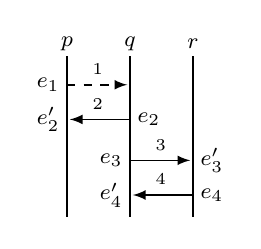
\begin{tikzpicture}[>=stealth,node distance=3.2cm,shorten >=1pt,
      every state/.style={text=black, scale =0.8}, semithick,
      font={\fontsize{8pt}{12}\selectfont}]
	\begin{scope}[xshift = 9cm, scale = 0.8]
		\node at (-0.3, -0.65)  (e)    {$e_1$};
		\node at (1.3, -1.2)  (e)    {$e_2$};
		\node at (-0.3, -1.2)  (e)    {$e_2'$};
		\node at (0.7, -1.85)  (e)    {$e_3$};
		\node at (2.3, -1.85)  (e)    {$e_3'$};
		\node at (2.3, -2.4)  (e)    {$e_4$};
		\node at (0.7, -2.4)  (e)    {$e_4'$};
		%MACHINES
		\draw (0,0) node{$p$} ;
		\draw (1,0) node{$q$} ;
		\draw (2,0) node{$r$} ;
		\draw (0,-0.2) -- (0,-2.8) ;
		\draw (1,-0.2) -- (1,-2.8);
		\draw (2, -0.2) -- (2, -2.8) ;
		%MESSAGES
		\draw[>=latex,->, dashed] (0,-0.65) -- (1, -0.65) node[midway,above]{$\amessage_1$};

		\draw[>=latex,->] (1, -1.2) -- (0, -1.2) node[midway, above] {$\amessage_2$};

		\draw[>=latex,->] (1,-1.85) -- (2,-1.85) node[midway, above] {$\amessage_3$};

		\draw[>=latex,->] (2,-2.4) -- (1,-2.4) node[midway,above] {$\amessage_4$};
	\end{scope}

\end{tikzpicture}
\captionof{figure}{MSC $\mscweakuniver$}
\label{fig:msc_weak_univer}
\end{center}
%\alain{NIce}
%\end{figure}

\end{minipage}

\paragraph*{Mailbox MSCs.}

For an MSC $\msc = (\Events,\procrel,\lhd,\lambda)$, we define
an additional binary relation that represents a constraint
under the mailbox semantics, where each process has only one incoming channel.
Let ${\mbrel}_\msc \subseteq \Events \times \Events$
be defined by: $e_1 \mbrel e_2$ if there is $q \in \Procs$
such that $\lambda(e_1) \in \qsAct{q}$,
$\lambda(e_2) \in \qsAct{q}$, and one of the following holds:
\begin{itemize}\itemsep=0.5ex
\item $e_1 \in \Matched{\msc}$ and $e_2 \in \Unm{\msc}$, or
\item $e_1 \lhd f_1$ and $e_2 \lhd f_2$ for some $f_1,f_2 \in \Events_q$ such that $f_1 \procrel^+ f_2$.
\end{itemize}

We let ${\mbpartial} = ({\procrel} \,\cup\, {\lhd} \,\cup\, {\mbrel})^\ast$.
Note that ${\le} \subseteq {\mbpartial}$.
%
%\begin{definition}\label{def:mailbox-msc}
We call $\msc \in \ppMSCs$ a \emph{mailbox MSC}
if ${\mbpartial}$ is a partial order.
%\end{definition}
Intuitively, this means that events can be scheduled in a way that corresponds
to the mailbox semantics, i.e., with one incoming channel per process.
Following the terminology in \cite{DBLP:conf/cav/BouajjaniEJQ18}, we also say that
a mailbox MSC satisfies \emph{causal delivery}.
The set of mailbox MSCs $\msc \in \ppMSCs$ is denoted by $\cdMSCs$.

\begin{example}\label{ex:mailbox-msc}
    MSC $\mscweakuniver$ is a mailbox MSC. Indeed, even though the order $\linrel$ defined in Example~\ref{ex:msc} does not respect all mailbox constraints, particularly the fact that $e_4 \mbrel^{(\mscweakuniver)} e_1$, there is a total order $ {\mblin} \supseteq {\mbpartial^{(\mscweakuniver)}}$ such that $
    e_2 \mblin e_3 \mblin e_3' \mblin e_4 \mblin e_1 \mblin e_2' \mblin e_4'$. We call $\mblin$ a mailbox linearization, which is formally defined below.
\end{example}

\paragraph*{Linearizations, Prefixes, and Concatenation.}

Consider $\msc = (\Events,\procrel,\lhd,\lambda) \in \MSCs$.
A \emph{\pp linearization} (or simply \emph{linearization}) of $\msc$ is a (reflexive) total order
${\linrel} \subseteq \Events \times \Events$ such that ${\le} \subseteq
{\linrel}$. Similarly,
a \emph{mailbox linearization} of $\msc$ is a total order
${\linrel} \subseteq \Events \times \Events$ such that ${\mbpartial} \subseteq
{\linrel}$. That is, every mailbox linearization is a \pp linearization,
but the converse is not necessarily true (Example~\ref{ex:mailbox-msc}).
Note that an MSC is a mailbox MSC iff it has at least one mailbox linearization.

\medskip

Let $\msc = (\Events,\procrel,\lhd,\lambda) \in \MSCs$ and consider
$E \subseteq \Events$ such that $E$ is ${\le}$-\emph{downward-closed}, i.e,
for all $(e,f) \in {\le}$ such that $f \in E$, we also have $e \in E$.
Then, the MSC $(E,{\procrel} \cap (E \times E),{\lhd} \cap (E \times E),\lambda')$,
where $\lambda'$ is the restriction of $\Events$ to $E$, is called a \emph{prefix}
of $\msc$. In particular, the empty MSC is a prefix of $\msc$.
We denote the set of prefixes of $\msc$ by $\Pref{\msc}$.
This is extended to sets $L \subseteq \MSCs$ as expected, letting
$\Pref{L} = \bigcup_{\msc \in L} \Pref{\msc}$.

\begin{lemma}
\label{lem:mb-prefix}
Every prefix of a mailbox MSC is a mailbox MSC.
\end{lemma}
\begin{proof}
Let $\msc = (\Events, \procrel, \lhd, \lambda) \in \mbMSCs$ and $\msc_0 =
(\Events_0, \procrel_0, \lhd_0, \lambda_0)$ be a prefix of $\msc$, i.e.,
$\Events_0 \subseteq \Events$. By contradiction, suppose that $\msc_0$ is not a
mailbox MSC. Then, there are distinct $e,f \in \Events_0$ such that $e \mbpartial^{(M_0)} f \mbpartial{(M_0)}
e$ with ${\mbpartial^{(\msc_0)}} = ({\rightarrow_0} \cup {\lhd_0} \cup {\mbrel^{(\msc_0)}})^*$.
As $\Events_0 \subseteq \Events$, we have that ${\rightarrow_0} \subseteq {\rightarrow}$, ${\lhd_0} \subseteq {\lhd}$, and ${\mbrel^{(\msc_0)}} \subseteq {\mbrel^{(\msc)}}$. Finally, ${\mbpartial^{(\msc_0)}} \subseteq {\mbpartial^{(\msc)}}$ and $\msc$ is not a mailbox MSC, which is a contradiction.
\end{proof}

Let $\msc_1 = (\Events_1,\procrel_1,\lhd_1,\lambda_1)$ and
$\msc_2 = (\Events_2,\procrel_2,\lhd_2,\lambda_2)$ be two MSCs.
Their \emph{concatenation} $\msc_1 \cdot \msc_2 = (\Events,\procrel,\lhd,\lambda)$ is defined if, for all $(p,q) \in \Ch$,
$e_1 \in \Unm{\msc_1}$, and
$e_2 \in \Events_2$ such that $\lambda(e_1) \in \pqsAct{p}{q}$
and $\lambda(e_2) \in \pqsAct{p}{q}$,
we have $e_2 \in \Unm{\msc_2}$.
As expected, $\Events$ is the disjoint union of $\Events_1$ and $\Events_2$,
${\lhd}  = {\lhd_1} \cup {\lhd_2}$, $\lambda$ is the ``union'' of $\lambda_1$
and $\lambda_2$, and ${\procrel} = {\procrel_1} \cup {\procrel_2} \cup R$.
Here, $R$ contains, for all $p \in \Procs$ such that $(\Events_1)_p$ and
$(\Events_2)_p$ are non-empty, the pair $(e_1,e_2)$ where $e_1$ is the
maximal $p$-event in $M_1$ and $e_2$ is the minimal $p$-event in $M_2$.
Note that $\msc_1 \cdot \msc_2$ is indeed an MSC and that
concatenation is associative.


% !TEX root = popl-paper.tex

\subsection{Communicating Systems}

We now recall the definition of communicating systems (aka communicating finite-state
machines or message-passing automata), which consist of finite-state machines $A_p$
(one for every process $p \in \Procs$) that can communicate through channels from $\Ch$. In our case, we consider the most general definition in which channels behave as bags, which means that no specific order is enforced on the delivery of messages.

\begin{definition}\label{def:cs}
A \emph{communicating system} over $\Procs$ and $\Msg$ is a tuple
   $ \Sys = (A_p)_{p\in\procSet}$. For each
   $p \in \Procs$, $A_p = (Loc_p, \delta_p, \ell^0_p)$ is a finite transition system where
   $\Loc_p$ is a finite set of local (control) states, $\delta_p
   \subseteq \Loc_p \times \pAct{p} \times \Loc_p$ is the
   transition relation, and $\ell^0_p \in Loc_p$ is the initial state.
\end{definition}

Given $p \in \Procs$ and a transition $t = (\ell,a,\ell') \in \delta_p$, we let
$\tsource(t) = \ell$, $\ttarget(t) = \ell'$, $\tlabel(t) = a$, and
$\tmessage(t) = \msg$ if $a \in \msAct{\msg} \cup \mrAct{\msg}$.

\smallskip

There are in general two ways to define the semantics of a communicating system.
Most often it is defined as a global infinite transition system that keeps track
of the various local control states and all (unbounded) channel contents.
As, in this paper, our arguments are based on a graph view of MSCs, we will define
the language of $\Sys$ directly as a set of MSCs. These two semantic views are essentially
equivalent, but they have different advantages depending on the context.
We refer to \cite{CyriacG14} for a thorough discussion.

\davidequestion{MSCs are formally defined in chapter 5... maybe move here in the preliminaries just the asynchronous definition?}
Let $\msc = (\Events,\procrel,\lhd,\lambda)$ be an MSC.
A \emph{run} of $\Sys$ on $\msc$ is a mapping
$\rho: \Events \to \bigcup_{p \in \Procs} \delta_p$
that assigns to every event $e$ the transition $\rho(e)$
that is executed at $e$. Thus, we require that
\begin{enumerate*}[label={(\roman*)}]
\item for all $e \in \Events$, we have $\tlabel(\rho(e)) = \lambda(e)$,
\item for all $(e,f) \in {\procrel}$, $\ttarget(\rho(e)) = \tsource(\rho(f))$,
\item for all $(e,f) \in {\lhd}$, $\tmessage(\rho(e)) = \tmessage(\rho(f))$,
and
\item for all $p \in \Procs$ and $e \in \Events_p$ such that there is no $f \in \Events$ with $f \procrel e$, we have $\tsource(\rho(e)) = \ell_p^0$.
\end{enumerate*}

Letting run $\Sys$ directly on MSCs is actually very convenient.
This allows us to associate with $\Sys$ its p2p language and mailbox language
in one go. The \emph{\pp language} of $\Sys$ is $\ppL{\Sys} = \{\msc \in \ppMSCs \mid$ there is a run of $\Sys$ on $\msc\}$.
The \emph{mailbox language} of $\Sys$ is $\mbL{\Sys} = \{\msc \in \mbMSCs \mid$ there is a run of $\Sys$ on $\msc\}$.

Note that, following \cite{DBLP:conf/cav/BouajjaniEJQ18,DBLP:conf/fossacs/GiustoLL20},
we do not consider final states or final configurations, as our purpose is to
reason about all possible
traces that can be \emph{generated} by $\Sys$.
%We will discuss this issue in more detail later in the paper. \todo{Do we still discuss this in the conference version or can we omit this sentence?}
The next lemma is obvious for the p2p semantics and follows from Lemma~\ref{lem:mb-prefix} for
	the mailbox semantics.

\begin{lemma}\label{lem:prefix-closed}
For all $\comsymb \in \{\ppsymb, \mbsymb\}$, $\cL{\Sys}$ is prefix-closed:
$\Pref{\cL{\Sys}} \subseteq \cL{\Sys}$.
\end{lemma}

\begin{example}
	Fig.~\ref{fig:system_weak_univer} depicts $\systemweakuniver = (A_p, A_q, A_r)$ such that MSC $\mscweakuniver$ in Fig.~\ref{fig:msc_weak_univer} belongs to $\ppL{\systemweakuniver}$ and to $\mbL{\systemweakuniver}$.
	There is a unique run $\rho$ of $\systemweakuniver$ on $\mscweakuniver$.
	We can see that $(e_3',e_4) \in {\rightarrow}$ and $\ttarget(\rho(e_3')) = \tsource(\rho(e_4)) = \ell_r^{1}$, $(e_2, e_2') \in \lhd_{\mscweakuniver}$, and $\tmessage(\rho(e_2)) = \tmessage(\rho(e_2')) = \msg_2$.
	\end{example}
	\begin{figure}[t]
	\begin{center}
	  \begin{tikzpicture}[>=stealth,node distance=3.2cm,shorten >=1pt,
		every state/.style={text=black, scale =0.75}, semithick,
		font={\fontsize{8pt}{12}\selectfont},
		scale = 0.9
		]
	  \begin{scope}[->]
		  \node[state,initial,initial text={}] (q0)  {$\ell_p^{0}$};
		  \node[state, right of=q0] (q1)  {$\ell_p^{1}$};
				\node[state, right of=q1] (q2) {$\ell_p^{2}$};

			\path (q0) edge node [above] {$\send{p}{q}{\msg_1}$} (q1);
				\path (q1) edge node [above] {$\rec{q}{p}{\msg_2}$}(q2);
			\node[thick] at (-1.1,0) {$A_p$};
	  \end{scope}

	  \begin{scope}[->, shift={(7.5,0)}]
		  \node[state,initial,initial text={}] (q0)  {$\ell_q^{0}$};
				\node[state, right of=q0] (q1)  {$\ell_q^{1}$};
				\node[state, below of=q1, node distance = 1.5cm] (q2) {$\ell_q^{2}$};
				\node[state, left of=q2] (q3)  {$\ell_q^{3}$};

				\path (q0) edge node [above] {$\send{q}{p}{\msg_2}$} (q1);
				\path (q1) edge node [right] {$\send{q}{r}{\msg_3}$}(q2);
				\path (q2) edge node [above] {$\rec{r}{q}{\msg_4}$} (q3);
				\node[thick] at (-1.1,0) {$A_q$};
	  \end{scope}

		\begin{scope}[->, shift={(0,-1.25)} ]
		  \node[state,initial,initial text={}] (q0)  {$\ell_r^{0}$};
				\node[state, right of=q0] (q1)  {$\ell_r^{1}$};
				\node[state, right of=q1] (q2) {$\ell_r^{2}$};

				\path (q0) edge node [above] {$\rec{q}{r}{\msg_3}$} (q1);
				\path (q1) edge node [above] {$\send{r}{q}{\msg_4}$}(q2);
				\node[thick] at (-1.1,0) {$A_r$};
	  \end{scope}
	\end{tikzpicture}
	\captionof{figure}{System $\systemweakuniver$}
	\label{fig:system_weak_univer}
	\end{center}
	\end{figure}

\subsection{Conflict Graph}

\davidequestion{The conflict graph is needed only for some proofs on the cuncur paper. I think it makes sense not to include it here and eventually introduce it later in the MSO-treewidth chapter if we really need it.}

We now recall the notion of a conflict graph associated to an MSC defined in \cite{DBLP:conf/cav/BouajjaniEJQ18}. This graph is used to depict the causal dependencies between message exchanges.  Intuitively, we have a dependency whenever
two messages have a process in common. For instance, an $\xrightarrow{SS}$
dependency between message exchanges $v$ and $v'$ expresses the fact that
$v'$ has been sent after $v$, by the same process. This notion is of interest because it was seen in \cite{DBLP:conf/cav/BouajjaniEJQ18} that the notion of synchronizability in MSCs (which is studied in this paper) can be graphically characterized by the nature of the associated conflict graph.
It is defined in terms of linearizations
in \cite{DBLP:conf/fossacs/GiustoLL20}, but we equivalently express it
directly in terms of MSCs.

For an MSC $\msc = (\Events, \rightarrow, \lhd, \lambda)$ and
$e \in \Events$, we define the type $\type(e) \in \{\stype,\rtype\}$ of $e$ by $\type(e) = \stype$ if $e \in \SendEv{\msc}$
and $\type(e) = \rtype$ if $e \in \RecEv{\msc}$.
Moreover, for $e \in \Unm{\msc}$, we let $\mexch(e) = e$,
and for $(e,e') \in \lhd$, we let $\mexch(e) = \mexch(e') = (e,e')$.


\begin{definition}[Conflict graph]
	The \emph{conflict graph} $\cgraph{\msc}$ of an MSC $\msc = (\Events, \rightarrow, \lhd, \lambda)$ is the labeled graph $(\Nodes, \Edges)$, with $\Edges \subseteq \Nodes \times \{\stype,\rtype\}^2 \times \Nodes$, defined by
	$\Nodes = {\lhd} \cup \Unm{\msc}$ and $\Edges = \{(\mu(e),\type(e)\type(f),\mu(f)) \mid (e,f) \in {\to^+}\}$.
In particular, a node of $\cgraph{\msc}$ is either a single unmatched send event or a message pair $(e,e') \in {\lhd}$.
\end{definition}

\subsection{Logic and Special treewidth}

\davidequestion{Special treewidth is used only in the final chapter, to me it makes more sense to introduce it there}

\paragraph*{Monadic Second-Order Logic.}
The set of MSO formulas over MSCs (over $\Procs$ and $\Msg$) is given by the grammar
$
\phi ::= x \procrel y \mid x \lhd y \mid \lambda(x) = a \mid x = y \mid x \in X \mid \exists x.\phi \mid \exists X.\phi \mid \phi \vee \phi \mid \neg \phi
$,
where $a \in \Act$, $x$ and $y$ are first-order variables, interpreted as
events of an MSC, and $X$ is a second-order variable, interpreted
as a set of events. We assume that we have an infinite supply of variables,
and we use common abbreviations such as $\wedge$, $\forall$, etc.
The satisfaction relation is defined in the standard way and self-explanatory.
For example, the formula $\neg\exists x.(\bigvee_{a \in \sAct} \lambda(x) = a \;\wedge\; \neg \mathit{matched}(x))$
with $\mathit{matched}(x) = \exists y.x \lhd y$
says that there are no unmatched send events.
It is not satisfied by  MSC $\mscweakuniver$
of Fig.~\ref{fig:msc_weak_univer},
as message $\msg_1$ is not received,
but by $\mscstrongexist$ from Fig.~\ref{fig:msc_strong_exist}.

Given a sentence $\phi$, i.e., a formula without free variables,
we let $L(\phi)$ denote the set of (p2p) MSCs that satisfy $\phi$.
%
It is worth mentioning that the (reflexive) transitive closure of
a binary relation defined by an MSO formula with free variables $x$ and $y$,
such as $x \procrel y$, is MSO-definable so that the logic can freely
use formulas of the form $x \procrel^+ y$ or $x \le y$ (where $\le$
is interpreted as $\le$ for the given MSC $\msc$).
Therefore, the definition of a mailbox MSC can be readily translated into
the formula $\mbformula = \neg \exists x.\exists y.(\neg (x = y) \wedge x \mbpartial y \wedge y \mbpartial x)$ so that we have $L(\mbformula) = \mbMSCs$.
Here, $x \mbpartial y$ is obtained as the MSO-definable reflexive transitive closure of
the union of the MSO-definable relations $\procrel$, $\lhd$, and $\sqsubset$.
In particular, we may define $x \sqsubset y$ by :
\[
x \sqsubset y =
\displaystyle
\hspace{-1em}\bigvee_{\substack{q \in \Procs\\a,b \in \qsAct{q}}}\hspace{-1em}
\lambda(x) = a \;\wedge\; \lambda(y) = b
\wedge
\left(
\begin{array}{rl}
& \mathit{matched}(x) \wedge \neg \mathit{matched}(y)\\[1ex]
\vee & \exists x'.\exists y'. (x \lhd x' \;\wedge\; y \lhd y' \;\wedge\; x' \procrel^+ y')
\end{array}
\right)
\]

\paragraph*{Special treewidth.}

\emph{Special treewidth} \cite{Courcelle10},
is a graph measure that indicates how close
a graph is to a tree (we may also use classical
	\emph{treewidth} instead).
This or similar measures are commonly employed in verification. For instance, treewidth and split-width have been used in \cite{MadhusudanP11} and, respectively, \cite{DBLP:conf/concur/CyriacGK12,AiswaryaGK14} to reason about graph behaviors generated by pushdown and queue systems.
%Here we apply it to reason about MSCs.
There are several ways to define the special treewidth of an MSC.
We adopt the following game-based definition from \cite{DBLP:journals/corr/abs-1904-06942}.

Adam and Eve play a two-player turn based ``decomposition game''
whose positions
are MSCs with some pebbles placed on some events.
More precisely, Eve's positions are
\emph{marked MSC fragments} $(M, U)$, where
$\msc = (\Events, \procrel, \lhd, \lambda)$
is an \emph{MSC fragment} (an MSC with possibly some edges from
$\lhd$ or $\to$ removed)
 and $U \subseteq \Events$ is the subset of marked events.
Adam's positions are pairs of marked MSC fragments.
A move by Eve consists in the following steps:
\begin{enumerate}
	\item marking some events of the MSC resulting in $(M, U')$ with $U \subseteq U' \subseteq \Events$,
	\item removing (process and/or message) edges whose endpoints are marked,
	\item dividing $(M, U)$ in $(M_1, U_1)$ and $(M_2, U_2)$ such that $M$ is the disjoint (unconnected) union of $M_1$ and $M_2$
	and marked nodes are inherited.
\end{enumerate}
When it is Adam's turn, he simply chooses one of the two marked MSC fragments.
The initial position is $(\msc,\emptyset)$ where $M$ is the (complete) MSC at hand. A terminal position is any position belonging to Eve such that all events are marked.
%
For $k \in \N$, we say that the game is $k$-winning for Eve if she has a (positional) strategy that allows her,
starting in the initial position and independently of Adam's moves, to reach a terminal position such that, in every single position visited along the play, there are at most $k+1$ marked events.

\begin{fact}[\cite{DBLP:journals/corr/abs-1904-06942}]
	The special treewidth of an MSC is the least $k$ such that
	the associated game is $k$-winning for Eve.
\end{fact}

The set of MSCs whose special treewidth is at most $k$ is denoted by $\stwMSCs{k}$.

\subsection{Definitions}

A Message Sequence Chart (MSC), such as the one in Fig.~\ref{}, provides a visual description of the behaviour of a distributed system. In this section, we start by formally defining the most generic class of Message Sequence Charts (MSCs), which we call asynchronous MSCs. More specialized classes of MSCs, such as $\pp$ MSCs, will also be discussed. Intuitively, we say that an MSC $\msc$ is asynchronous if there is an asynchronous system $\System$ that can exhibit the behaviour described by $\msc$.

\begin{definition}[Asynchronous MSC]
An \emph{asynchronous MSC} (or simply MSC) over $\Procs$ and $\Msg$ is a tuple $\msc = (\Events,\procrel,\lhd,\lambda)$, where $\Events$ is a finite (possibly empty) set of \emph{events} and $\lambda: \Events \to \Act$ is a labeling function that associates an action to each event. For $p \in \Procs$, let $\Events_p = \{e \in \Events \mid \lambda(e) \in \pAct{p}\}$ be the set of events that are executed by $p$. We require that $\procrel$ (the \emph{process relation}) is the disjoint union $\bigcup_{p \in \Procs} \procrel_p$ of relations ${\procrel_p} \subseteq \Events_p \times \Events_p$ such that $\procrel_p$ is the direct successor relation of a total order on $\Events_p$. For an event $e \in \Events$, a set of actions $A \subseteq \Act$, and a relation $\rel \subseteq \Events \times \Events$,
let $\sametype{e}{A}{\rel} = |\{f \in \Events \mid (f,e) \in \rel$ and $\lambda(f) \in A\}|$. We require that ${\lhd} \subseteq \Events \times \Events$ (the \emph{message relation}) satisfies the following:
\begin{itemize}\itemsep=0.5ex
\item[(1)] for every pair $(e,f) \in {\lhd}$, there is a send action $\sact{p}{q}{\msg} \in \Act$ such that $\lambda(e) = \sact{p}{q}{\msg}$, $\lambda(f) = \ract{p}{q}{\msg}$.
\item[(2)] for all $f \in \Events$ such that $\lambda(f)$ is a receive action, there is exactly one $e \in \Events$ such that $e \lhd f$.
\end{itemize}
Finally, letting ${\le}_\msc = ({\procrel} \cup {\lhd})^\ast$,
we require that $\le$ is a partial order. For convenience, we simply write $\le$ when $M$ is clear from the context. We will refer to $\le$ as the \emph{causal ordering} or \emph{happens-before} relation. If, for two events $e$ and $f$, we have that $e \le f$, we will equivalently say that there is a \emph{causal path} between $e$ and $f$.
\end{definition}

According to Condition (2), every receive event must have a matching send event. Note that, however, there may be unmatched send events.
We let
$\SendEv{\msc} = \{e \in \Events \mid \lambda(e)$ is a send
action$\}$,
$\RecEv{\msc} = \{e \in \Events \mid \lambda(e)$ is a receive
action$\}$,
$\Matched{\msc} = \{e \in \Events \mid$ there is $f \in \Events$
such that $e \lhd f\}$, and
$\Unm{\msc} = \{e \in \Events \mid \lambda(e)$ is a send
action and there is no $f \in \Events$ such that $e \lhd f\}$.
%
We do not distinguish isomorphic MSCs and
let $\asMSCs$ be the set of all the asynchronous MSCs over the given sets $\Procs$ and $\Msg$.

% \paragraph*{Linearizations.}

% Consider $\msc = (\Events,\procrel,\lhd,\lambda) \in \asMSCs$.
% An \emph{asynchronous linearization} of $\msc$ is a (reflexive) total order ${\linrel} \subseteq \Events \times \Events$ such that ${\le} \subseteq {\linrel}$. Intuitively, an asynchronous linearization of $\msc$ is a possible ordering of its events.
% \davide{Example of asynchronous linearization.}

\paragraph*{Linearizations.}

Consider $\msc = (\Events,\procrel,\lhd,\lambda) \in \asMSCs$.
A \emph{linearization} of $\msc$ is a (reflexive) total order ${\linrel} \subseteq \Events \times \Events$ such that ${\le} \subseteq {\linrel}$. In other words, a linearization of $\msc$ is a total order that respects the happens-before relation $\le$ defined over $\msc$.
\davide{Provide example of linearization.}

\medskip

Asynchronous MSCs are the widest class of MSCs that we will deal with. By introducing additional constraints, we are able to define other classes of MSCs that exclusively describe the behaviours of \pp systems, mailbox systems, and so on.
\davide{Provide example of asynchronous MSC that is not p2p.}

As in the asynchronous case, we say that $\msc$ is a \pp MSC if there is a \pp system that can produce the behaviour described by $\msc$. We give here the formal definition of \pp MSC, which also considers the possibility of having unmatched messages (i.e. messages that are sent but not received).
\davideanswer{Why unmatched messages? What do they represent? When an automata does not have the receive action for a message that was already sent (see examples at the end of concur paper).}

\begin{definition}[Peer-to-peer MSCs]
A \emph{\pp MSC} (or simply \emph{MSC}) is an asynchronous MSC where we require that, for every pair $(e,f) \in {\lhd}$, such that $\lambda(e) = \sact{p}{q}{\msg}$, $\lambda(f) = \ract{p}{q}{\msg}$, we have $\sametype{e}{\pqsAct{p}{q}}{\procrel^+} = \sametype{f}{\pqrAct{p}{q}}{\procrel^+}$.
\end{definition}

The additional constraint satisfied by \pp MSCs ensures that channels operate in FIFO mode; when a process $q$ receives a message from a process $p$, it must have already received all the messages that were previously sent to him by $p$. Let $\ppMSCs$ denote the set of all the \pp MSCs over two given sets $\Procs$ and $\Msg$. Note that, by definition, every \pp MSC is an asynchronous MSC. The idea is that we are always able to find an asynchronous system that \emph{can} exhibit the behaviour described by a \pp MSC; after all, the channels of an asynchronous system do not have to follow any specific behaviour, so they can indeed happen to operate as if they were queues. Example~\ref{} shows that the opposite direction is generally not true, an asynchronous MSC is not always a \pp MSC. It follows that $\ppMSCs \subset \asMSCs$.

\medskip

We will now consider the class of MSCs for which there is a causally ordered system that can produce their behaviour. Intuitively, an MSC is causally ordered if all the messages sent to the same process are received in an order which is consistent with the causal ordering of the corresponding send events. Below the formal definition, which also considers unmatched messages.
\davide{Provide example of an MSC that is not causally ordered}
\begin{definition}[Causally ordered MSC]
An MSC $\msc = (\Events,\procrel,\lhd,\lambda)$ is \emph{causally ordered} if, for any two send events $s$ and $s'$, such that $\lambda(s)=\pqsAct{\plh}{q}$, $\lambda(s')=\pqsAct{\plh}{q}$, and $s \le s'$, we have either:
\begin{itemize}\itemsep=0.5ex
	\item $s,s' \in \Matched{\msc}$ and $r \procrel^* r'$, where $r$ and $r'$ are two receive events such that $s \lhd r$ and $s' \lhd r'$.
	\item $s' \in \Unm{\msc}$.
\end{itemize}
\end{definition}

By definition, every causally ordered MSC is a \pp MSC. This is not surprising, considering that a causally ordered system is essentially a \pp system with an additional constraint on the delivery of messages; indeed, we are always able to find a \pp system that \emph{can} exhibit the behaviour described by a causally ordered MSC. Let $\coMSCs$ denote the set of all the causally ordered MSCs over two given sets $\Procs$ and $\Msg$. Example~\ref{} shows that a \pp MSC is not always a causally ordered MSC. It follows that $\coMSCs \subset \ppMSCs$.

\medskip

Moving on to the mailbox semantics, we say that $\msc$ is a mailbox MSC if there is a mailbox system that can exhibit the behaviour described by $\msc$.
\davide{Provide example of MSC which is not mailbox}

\begin{definition}[Mailbox MSC]% \label{def:mb_msc}
An MSC $\msc = (\Events,\procrel,\lhd,\lambda)$ is a \emph{mailbox MSC} if it has a linearization $\linrel$ where, for any two send events $s$ and $s'$, such that $\lambda(s)=\pqsAct{\plh}{q}$, $\lambda(s')=\pqsAct{\plh}{q}$, and $s \linrel s'$, we have either:
\begin{itemize}\itemsep=0.5ex
	\item $s,s' \in \Matched{\msc}$ and $r \linrel r'$, where $r$ and $r'$ are two receive events such that $s \lhd r$ and $s' \lhd r'$.
	\item $s' \in \Unm{\msc}$.
\end{itemize}
\end{definition}

Such a linearization will be referred to as a \emph{mailbox linearization}, and the symbol $\mblinrel$ will be used to denote one. Let $\mbMSCs$ denote the set of all the mailbox MSCs over two given sets $\Procs$ and $\Msg$. By definition, every mailbox MSC is a \pp MSC. Conversely, Example~\ref{} shows a \pp MSC which is not a mailbox MSC. It follows that $\mbMSCs \subset \ppMSCs$. We show here that each mailbox MSC is also a causally ordered MSC.
\davide{Provide example of causally ordered MSC which is not mailbox (Fig.~2.18 of Laetitia's thesis).}

\begin{proposition}% \label{prop:mb_is_co}
	Every mailbox MSC is a causally ordered MSC.
\end{proposition}
\begin{proof}
Let $\msc$ be a mailbox MSC and $\linrel$ a mailbox linearization of it. Recall that a linearization has to respect the happens-before partial order over $\msc$, i.e. $\le \,\subseteq\, \linrel$. Consider any two send events $s$ and $s'$, such that $\lambda(s)=\pqsAct{\plh}{q}$, $\lambda(s')=\pqsAct{\plh}{q}$ and $s \le s'$. Since $\le \,\subseteq\, \linrel$, we have that $s \linrel s'$ and, by the definition of mailbox linearization, either
\begin{enumerate*}[label={(\roman*)}]
	\item $s' \in \Unm{\msc}$, or
	\item $s,s' \in \Matched{\msc}$, $s \lhd r$, $s' \lhd r'$ and $r \linrel r'$.
\end{enumerate*}
The former clearly respects the definition of causally ordered MSC, so let us focus on the latter. Note that $r$ and $r'$ are two receive events executed by the same process, hence $r \linrel r'$ implies $r \procrel^+ r'$. It follows that $\msc$ is a causally ordered MSC.
\end{proof}

\medskip

Moving on to the $\onen$ semantics, we say that $\msc$ is a $\onen$ MSC if there is a $\onen$ system that can exhibit the behaviour described by $\msc$.

\begin{definition}[$\onen$ MSC]% \label{def:one_n}
An MSC $\msc = (\Events,\procrel,\lhd,\lambda)$ is a \emph{$\onen$ MSC} if it has a linearization $\linrel$ where, for any two send events $s$ and $s'$, such that $\lambda(s)=\pqsAct{p}{\plh}$, $\lambda(s')=\pqsAct{p}{\plh}$, and $s \procrel^+ s'$ (which implies $s \linrel s'$), we have either:
\begin{itemize}\itemsep=0.5ex
	\item $s,s' \in \Matched{\msc}$ and $r \linrel r'$, where $r$ and $r'$ are two receive events such that $s \lhd r$ and $s' \lhd r'$.
	\item $s' \in \Unm{\msc}$.
\end{itemize}
\end{definition}

Such a linearization will be referred to as a \emph{$\onen$ linearization}. Note that the definition is very similar to the mailbox case, but here $s$ and $s'$ are two send events executed by the same process. Let $\onenMSCs$ denote the set of all the $\onen$ MSCs over two given sets $\Procs$ and $\Msg$. By definition, every $\onen$ MSC is a \pp MSC. Conversely, Example~\ref{} shows a \pp MSC which is not a $\onen$ MSC. It follows that $\mbMSCs \subset \ppMSCs$. We show here that each $\onen$ MSC is also a causally ordered MSC, which is not as intuitive as the mailbox case.

\davide{Provide example of MSC which is not $\onen$}

\davidequestion{Should I still leave this proof if we showed that every $\onen$ MSC is a mailbox MSC?}
\begin{proposition}% \label{prop:onen_is_co}
	Every $\onen$ MSC is a causally ordered MSC.
\end{proposition}
\begin{proof}
By contradiction. Suppose that $\msc$ is a $\onen$ MSC, but not a causally ordered MSC. Since $\msc$ is not causally ordered, there must be two send events $s$ and $s'$ such that $\lambda(s)=\pqsAct{\plh}{q}$, $\lambda(s')=\pqsAct{\plh}{q}$, $s \le s'$, and we have either:
\begin{enumerate}\itemsep=0.5ex
	\item $s,s' \in \Matched{\msc}$ and $r' \procrel^* r$, where $r$ and $r'$ are two receive events such that $s \lhd r$ and $s' \lhd r'$.
	\item  $s \in \Unm{\msc}$ and $s' \in \Matched{\msc}$.
\end{enumerate}
We need to show that both of these scenarios lead to a contradiction. (1) Suppose $s$ and $s'$ are executed by the same process. Since $\msc$ is a $\onen$ MSC, there must be a linearization $\linrel$ such that $r \linrel r'$, but this is clearly impossible since we have $r' \procrel^* r$. Suppose now that $s$ and $s'$ are executed by two different processes $p$ and $q$. We know by hypothesis that $s \le s'$, i.e. there is a causal path of events $P = s \sim a \sim \dots \sim s' \sim r'$ from $s$ to $r'$, where $\sim$ is either $\procrel$ or $\lhd$. Refer to the first example in Fig.~\ref{fig:onen_is_co} for a visual representation ($P$ is drawn in purple). To have a causal path $P$, there must be a send event $s''$ that is executed by $p$ after $s$ and that is part of $P$, along with its receipt $r''$ (i.e. $P = s \le s'' \lhd r'' \le s' \lhd r'$). We clearly have $r'' \linrel r'$ for any linearization of $\msc$, because $r'' \le r'$ (they are both in the causal path $P$ and $r''$ happens before $r$). Since $\msc$ is a $\onen$ MSC, there has to be a linearization $\linrel$ where $r \linrel r''$, because $s$ and $s''$ are send events executed by the same process. It follows that $\msc$ should have a linearization were $r \linrel r'' \linrel r'$, but this is not possible because of the hypothesis that $r' \procrel^* r$. This is a contradiction. (2) Suppose $s$ and $s'$ are executed by the same process. It is trivial to see, by definition, that $\msc$ cannot be a $\onen$ MSC. Suppose now that $s$ and $s'$ are executed by two different processes $p$ and $q$, and consider the same send event $s''$ as before (executed by $p$). Refer to the second example in Figure~\ref{fig:onen_is_co} for a visual representation. Since $s''$ is matched, we have two events $s$ and $s''$, sent by the same process $p$, that are unmatched and matched, respectively. Clearly, $\msc$ cannot be a $\onen$ MSC.
\end{proof}

\begin{figure}[h]
	\centering
	\begin{subfigure}[b]{0.4\textwidth}
		\begin{center}
			\begin{tikzpicture}
				\newproc{0}{p}{-2.1};
				\newproc{1}{t}{-2.1};
				\newproc{2}{q}{-2.1};

				% \newmsgdiagnoname{0}{1}{-0.2}{-2.5}{black};
				\newmsgnoname{0}{1}{-0.3}{black};
				\newmsgnoname{0}{2}{-1}{black};
				\newmsgnoname{2}{1}{-1.7}{black};

				\newevent{black}{0}{-0.3}{s}{left};
				\newevent{black}{0}{-1}{s''}{left};
				\newevent{black}{2}{-1}{r''}{above right};
				\newevent{black}{1}{-1.7}{r'}{above right};
				\newevent{black}{2}{-1.7}{s'}{right};
				\newevent{black}{1}{-0.3}{r}{right};

				\newflechevert{Purple}{0}{-0.3}{-1};
				\newflechehor{Purple}{-1}{0}{2};
				\newflechevert{Purple}{2}{-1}{-1.7};
				\newflechehorinverse{Purple}{-1.7}{2}{1};

			\end{tikzpicture}
		\end{center}
	\end{subfigure}
	% \hfill
	\begin{subfigure}[b]{0.4\textwidth}
		\begin{center}
			\begin{tikzpicture}
				\newproc{0}{p}{-2.1};
				\newproc{1}{t}{-2.1};
				\newproc{2}{q}{-2.1};

				% \newmsgdiagnoname{0}{1}{-0.2}{-2.5}{black};
				\newmsgumnoname{0}{1}{-0.3}{black};
				\newmsgnoname{0}{2}{-1}{black};
				\newmsgnoname{2}{1}{-1.7}{black};

				\newevent{black}{0}{-0.3}{s}{left};
				\newevent{black}{0}{-1}{s''}{left};
				\newevent{black}{2}{-1}{r''}{above right};
				\newevent{black}{2}{-1.7}{s'}{right};
				\newevent{black}{1}{-1.7}{r'}{above right};

				\newflechevert{Purple}{0}{-0.3}{-1};
				\newflechehor{Purple}{-1}{0}{2};
				\newflechevert{Purple}{2}{-1}{-1.7};
				\newflechehorinverse{Purple}{-1.7}{2}{1};

			\end{tikzpicture}
			\end{center}
	\end{subfigure}
	   \caption{Two examples of $\onen$ MSCs.}
	   % \label{fig:onen_is_co}
\end{figure}

\davide{Provide example of causally ordered MSC which is not $\onen$ (same as mailbox! Figure 2.18 of Laetitia's thesis).}

\begin{definition} [$\onen$ alternative]% \label{def:one_n_alt}
For an MSC $\msc = (\Events,\procrel,\lhd,\lambda)$, we define
an additional binary relation that represents a constraint
under the $\onen$ semantics, which ensures that messages sent from the same process are received in the same order. Let ${\onenrel}_\msc \subseteq \Events \times \Events$ be defined as $e_1 \onenrel e_2$ if there are two events $e_1$ and $e_2$, and $p \in \Procs$ such that either:
\begin{itemize}\itemsep=0.5ex
	\item $\lambda(e_1) \in \psAct{p}$, $\lambda(e_2) \in \psAct{p}$, $e_1 \in \Matched{\msc}$, and $e_2 \in \Unm{\msc}$, or
	\item $\lambda(e_1) \in \prAct{p}$, $\lambda(e_2) \in \prAct{p}$, $s_1 \lhd e_1$ and $s_2 \lhd e_2$ for some $s_1,s_2 \in \Events_p$, and $s_1 \procrel^+ s_2$.
\end{itemize}

We let ${\onenpartial} = ({\procrel} \,\cup\, {\lhd} \,\cup\, {\onenrel})^\ast$.
Note that ${\le} \subseteq {\onenpartial}$.
%
%\begin{definition}% \label{def:mailbox-msc}
	We call $\msc \in \asMSCs$ a \emph{$\onen$ MSC}
	if ${\onenpartial}$ is a partial order.
\end{definition}

\davidequestion{Should I also include the proof that every mailbox MSC without unmatched messages is $\onen$? Do we need it?}

\begin{proposition}% \label{prop:onen_mb_no_unmatched}
	Every $\onen$ MSC without unmatched messages is a mailbox MSC.
\end{proposition}
\begin{proof}
We show that the contrapositive is true, i.e. if an MSC is not mailbox (and it does not have unmatched messages), it is also not $\onen$. Suppose $\msc$ is an asynchronous MSC, but not mailbox. There must be a cycle $\xi$ such that  $e \mbpartial e$, for some event $e$. Recall that ${\mbpartial} = ({\procrel} \,\cup\, {\lhd} \,\cup\, {\mbrel})^\ast$ and ${\le} = ({\procrel} \cup {\lhd})^\ast$. We can always explicitely write a cycle $e \mbpartial e$ only using $\mbrel$ and $\le$. For instance, there might be a cycle $e \mbpartial e$ because we have that $e \mbrel f \le g \mbrel h \mbrel i \le e$. Consider any two adiacent events $s_1$ and $s_2$ in the cycle $\xi$, where $\xi$ has been written using only $\mbrel$ and $\le$, and we never have two consecutive $\le$\footnote{This is always possible, since $a \le b \le c$ is written as $a \le c$.}. We have two cases:
\begin{enumerate}
	\item $s_1 \mbrel s_2$. We know, by definition of $\mbrel$, that $s_1$ and $s_2$ must be two send events and that $r_1 \procrel^+ r_2$, where $r_1$ and $r_2$ are the receive events that match with $s_1$ and $s_2$, respectively (we are not considering unmatched messages by hypothesis).
	\item $s_1 \le s_2$. Since $\msc$ is asynchronous by hyphotesis, $\xi$ has to contain at least one $\mbrel$\footnote{If that was not the case, $\le$ would also be cyclic and $\msc$ would not be an asynchronous MSC.}; recall that we also wrote $\xi$ in such a way that we do not have two consecutive $\le$. It is not difficult to see that $s_1$ and $s_2$ have to be send events, since they belong to $\xi$. We have two cases:
	\begin{enumerate}
		\item $r_1$ is in the causal path, i.e. $s_1 \lhd r_1 \le s_2$. In particular, note that $r_1 \le r_2$.
		\item $r_1$ is not in the causal path, hence there must be a message $m_k$ sent by the same process that sent $s_1$, such that $s_1 \procrel^+ s_k \lhd r_k \le s_2 \lhd r_2$, where $s_k$ and $r_k$ are the send and receive events associated with $m_k$, respectively. Since messages $m_1$ and $m_k$ are sent by the same process and $s_1 \procrel^+ s_k$, we should have $r_1 \onenrel r_k$, according to the $\onen$ semantics. In particular, note the we have $r_1 \onenrel r_k \le r_2$.
	\end{enumerate}
	In both case (a) and (b), we conclude that $r_1 \onenpartial r_2$. Recall that ${\onenpartial} = ({\procrel} \,\cup\, {\lhd} \,\cup\, {\onenrel})^\ast$.
\end{enumerate}
Notice that, for either cases, a relation between two send events $s_1$ and $s_2$ (i.e. $s_1 \mbrel s_2$ or $s_1 \le s_2$) always implies a relation between the respective receive events $r_1$ and $r_2$, according to the $\onen$ semantics. It follows that $\xi$, which is a cycle for the $\mbpartial$ relation, always implies a cycle for the $\onenpartial$ relation\footnote{If $\onenpartial$ is cyclic, $\msc$ is not a $\onen$ MSC.}, as shown by the following example. Let $\msc$ be a non-mailbox MSC, and suppose we have a cycle $s_1 \mbrel s_2 \mbrel s_3 \le s_4 \mbrel s_5 \le s_1$. $s_1 \mbrel s_2$ falls into case (1), so it implies $r_1 \procrel^+ r_2$. The same goes for $s_2 \mbrel r_3$, which implies $r_2 \procrel^+ r_3$. $s_3 \le s_4$ falls into case (2), and implies that $r_3 \onenpartial r_4$. $s_4 \mbrel s_5$ falls into case (1) and it implies $r_4 \procrel^+ r_5$. $s_5 \le s_1$ falls into case (2) and implies that $r_5 \onenpartial r_1$. Putting all these implications together, we have that $r_1 \procrel^+ r_2 \procrel^+ r_3 \onenpartial r_4 \procrel^+ r_5 \onenpartial r_1$, which is a cycle for $\onenpartial$. Note that, given any cycle for $\mbpartial$, we are always able to apply this technique to obtain a cycle for $\onenpartial$.
\end{proof}

Proposition~\ref{prop:onen_mb_no_unmatched} remains true even if we consider unmatched messages.

\begin{proposition}% \label{prop:onen_mb_unmatched}
	Every $\onen$ MSC is a mailbox MSC.
\end{proposition}
\begin{proof}
Let $\msc$ be an asynchronous MSC. The proof proceeds in the same way as the one of Proposition~\ref{prop:onen_mb_no_unmatched}, but unmatched messages introduce some additional cases. Consider any two adiacent events $s_1$ and $s_2$ in a cycle $\xi$ for $\mbpartial$, where $\xi$ has been written using only $\mbrel$ and $\le$, and we never have two consecutive $\le$. These are some additional cases:
\begin{enumerate}\setcounter{enumi}{2}
	\item $u_1 \mbrel s_2$, where $u_1$ is the send event of an unmatched message. This case never happens because of how $\mbrel$ is defined.
	\item $u_1 \le u_2$, where $u_1$ and $u_2$ are both send events of unmatched messages. Since both $u_1$ and $u_2$ are part of the cycle $\xi$, there must be an event $s_3$ such that $u_1 \le u_2 \mbrel s_3$. However, $u_2 \mbrel s_3$ falls into case (3), which can never happen.
	\item $u_1 \le s_2$, where $u_1$ is the send event of an unmatched message and $s_2$ is the send event of a matched message. Since we have a causal path between $u_1$ and $s_2$, there has to be a message $m_k$, sent by the same process that sent $m_1$, such that $u_1 \procrel^+ s_k \lhd r_k \le s_2 \lhd r_2$\footnote{Note that we can have $m_k = m_2$}, where $s_k$ and $r_k$ are the send and receive events associated with $m_k$, respectively. Since messages $m_1$ and $m_k$ are sent by the same process and $m_1$ is unmatched, we should have $s_k \onenrel u_1$, according to the $\onen$ semantics, but $u_1 \procrel^+ s_k$. It follows that if $\xi$ contains $u_1 \le s_2$, we can immediately conclude that $\msc$ is not a $\onen$ MSC.
	\item $s_1 \mbrel u_2$,  where $s_1$ is the send event of a matched message and $u_2$ is the send event of an unmatched message. Since both $s_1$ and $u_2$ are part of a cycle, there must be an event $s_3$ such that $s_1 \mbrel u_2 \le s_3$; we cannot have $u_2 \mbrel s_3$, because of case (3). $u_2 \le s_3$ falls into case (5), so we can conclude that $\msc$ is not a $\onen$ MSC.
\end{enumerate}
We showed that cases (3) and (4) can never happen, whereas cases (5) and (6) both imply that $\msc$ is not $\onen$. If we combine them with the cases described in Proposition~\ref{prop:onen_mb_no_unmatched} we have the full proof.
\end{proof}

\begin{definition}[$\nn$ MSC]% \label{def:n_n}
	An MSC $\msc = (\Events,\procrel,\lhd,\lambda)$ is a \emph{$\nn$ MSC} if it has a linearization $\linrel$ where, for any two send events $s$ and $s'$, such that $s \linrel s'$, we have either:
	\begin{itemize}\itemsep=0.5ex
		\item $s,s' \in \Matched{\msc}$ and $r \linrel r'$, where $r$ and $r'$ are two receive events such that $s \lhd r$ and $s' \lhd r'$.
		\item $s' \in \Unm{\msc}$.
	\end{itemize}
\end{definition}

Such a linearization will be referred to as a \emph{$\nn$ linearization}. Intuitively, with an $\nn$ MSC we are always able to schedule events in such a way that messages are received in the same order as they were sent, and unmatched messages are sent only after all matched messages are sent. By definition, every $\nn$ MSC is a $\onen$ MSC.

\begin{definition} [$\nn$ alternative]% \label{def:n_n_alt}
For an MSC $\msc = (\Events,\procrel,\lhd,\lambda)$, let ${\nnrel}_\msc = ({\procrel} \,\cup\, {\lhd} \,\cup\, {\mbrel} \,\cup\, {\onenrel})^\ast$. We define an additional binary relation $\nnbowtieofmsc\msc \subseteq \Events \times \Events$, such that for two events $e_1$ and $e_2$ we have $e_1 \nnbowtieofmsc\msc e_2$ if one of the following holds:
\begin{enumerate}\itemsep=0.5ex
	\item $e_1 \nnrelofmsc{\msc} e_2$
	\item $\lambda(e_1) \in \prAct{\plh}$, $\lambda(e_2) \in \prAct{\plh}$, $s_1 \lhd e_1$ and $s_2 \lhd e_2$ for some $s_1,s_2 \in \Events$, $s_1 \nnrelofmsc{\msc} s_2$ and $e_1 \notnnrelofmsc\msc e_2$.
	\item $\lambda(e_1) \in \psAct{\plh}$, $\lambda(e_2) \in \psAct{\plh}$, $e_1 \lhd r_1$ and $e_2 \lhd r_2$ for some $r_1,r_2 \in \Events$, $r_1 \nnrelofmsc{\msc} r_2$ and $e_1 \notnnrelofmsc\msc e_2$.
	\item $e_1 \in \Matched{\msc}$, $e_2 \in \Unm{\msc}$, $e_1 \notnnrelofmsc\msc e_2$.
\end{enumerate}

Note that $\mbpartial \subseteq \nnrelofmsc{\msc}$, $\onenpartial \subseteq \nnrelofmsc{\msc}$, and $\nnrelofmsc{\msc} \subseteq\; \nnbowtieofmsc\msc$. We call $\msc \in \asMSCs$ a \emph{$\nn$ MSC}
if ${\nnbowtieofmsc\msc}$ is acyclic.
\davidequestion{Initially I said "We call $\msc \in \asMSCs$ a \emph{$\nn$ MSC} if ${\nnbowtieofmsc\msc}$ is a partial order", but I don't think it is true, since $\nnbowtieofmsc\msc$ does not have to be transitive.}
\end{definition}

It is not trivial to see that Definition~\ref{def:n_n_alt} is equivalent to Definition~\ref{def:n_n}. To show that, we need some preliminary results and definitions.

\begin{proposition}
	Let $\msc$ be an MSC. Given two matched send events $s_1$ and $s_2$, and their respective receive events $r_1$ and $r_2$, $r_1 \nnbowtieofmsc\msc r_2 \implies s_1 \nnbowtieofmsc\msc s_2$.
\end{proposition}
\begin{proof}
Follows from the definition of $\nnbowtieofmsc\msc$. We have $r_1 \nnbowtieofmsc\msc r_2$ if either:
\begin{itemize}\itemsep=0.5ex
	\item $r_1 \nnrelofmsc{\msc} r_2$. Two cases: either \begin{enumerate*}[label={(\roman*)}]
		\item $s_1 \nnrelofmsc{\msc} s_2$, or
		\item $s_1 \notnnrelofmsc\msc s_2$.
	\end{enumerate*}
	The first case clearly implies $s_1 \nnbowtieofmsc\msc s_2$, for rule 1 in the definition of $\nnbowtieofmsc\msc$. The second too, because of rule 3.
	\item  $r_1 \notnnrelofmsc\msc r_2$, but $r_1 \nnbowtieofmsc\msc r_2$. This is only possible if rule 2 in the definition of $\nnbowtieofmsc\msc$ was used, which implies $s_1 \nnrelofmsc{\msc} s_2$ and, for rule 1, $s_1 \nnbowtieofmsc\msc s_2$.
\end{itemize}
\end{proof}

\begin{proposition}% \label{prop:n_n_cycl}
	Let $\msc$ be an MSC. If $\nnbowtieofmsc\msc$ is cyclic, then $\msc$ is not $\nn$.
\end{proposition}
\begin{proof}
Since a $\nn$ MSC is always both a mailbox and a $\onen$ MSC, it is clear that the cyclicity of $\nnrelofmsc{\msc}$ implies that $\msc$ is not $\nn$, because it means that we are not even able to find a linearization that is both mailbox and $\onen$. Moreover, since in a $\nn$ linearization the order in which messages are sent matches the order in which they are received, and unmatched send events can be executed only after matched send events, a $\nn$ MSC always has to satisfy the constraints imposed by the $\nnbowtieofmsc\msc$ relation. If $\nnbowtieofmsc\msc$, then for sure there is no $\nn$ linearization for $\msc$.
\end{proof}

Let the \emph{Event Dependency Graph} (EDG) of a $\nn$ MSC $\msc$ be a graph that has events as nodes and an edge between two events $e_1$ and $e_2$ if $e_1 \nnbowtieofmsc\msc e_2$. We now present an algorithm that, given the EDG of an $\nn$ MSC $\msc$, computes a $\nn$ linearization of $\msc$. We then show that, if $\nnbowtieofmsc\msc$ is acyclic (i.e. it is a partial order), this algorithm always terminates correctly. This, along with Proposition~\ref{prop:n_n_cycl}, effectively shows that Definition~\ref{def:n_n} and Definition~\ref{def:n_n_alt} are equivalent.

\paragraph*{Algorithm for finding a $\nn$ linearization}
The input of this algorithm is the EDG of an MSC $\msc$, and it outputs a valid $\nn$ linearization for $\msc$, if $\msc$ is $\nn$. The algorithm works as follows:
\begin{enumerate}
	\item If there is a matched send event $s$ with in-degree 0 in the EDG, add $s$ to the linearization and remove it from the EDG, along with its outgoing edges, then jump to step 5. Otherwise, proceed to step 2.
	\item If there are no matched send events in the EDG and there is an unmatched send event $s$ with in-degree 0 in the EDG, add $s$ to the linearization and remove it from the EDG, along with its outgoing edges, then jump to step 5. Otherwise, proceed to step 3.
 	\item If there is a receive event $r$ with in-degree 0 in the EDG, such that $r$ is the receive event of the first message whose sent event was already added to the linearization, add $r$ to the linearization and remove it from the EDG, along with its outgoing edges, then jump to step 5. Otherwise, proceed to step 4.
   	\item Throw an error and terminate.
   	\item If all the events of $\msc$ were added to the linearization, return the linearization and terminate. Otherwise, go back to step 1.
\end{enumerate}

We now need to show that
\begin{enumerate*}[label={(\roman*)}]
	\item if this algorithm terminates correctly (i.e. step 4 is never executed), it returns a $\nn$ linearization, and
	\item if $\nnbowtieofmsc\msc$ is acyclic, the algorithm always terminates correctly.
\end{enumerate*}
\begin{proposition}
	If the above algorithm returns a linearization for an MSC $\msc$, it is a $\nn$ linearization.
\end{proposition}
\begin{proof}
	Note that, because of how step 2 works, the order (in the linearization) in which matched messages are sent is the same as the order in which they are received. Moreover, according to step 3, an unmatched send events is added to the linearization only if all the matched send events were already added.
\end{proof}

\begin{proposition}
	Given an MSC $\msc$, the above algorithm always terminates correctly if $\nnbowtieofmsc\msc$ is acyclic.
\end{proposition}
\begin{proof}
We want to prove that, if $\nnbowtieofmsc\msc$ is acyclic, step 4 of the algorithm is never executed, i.e. it terminates correctly. Note that the acyclicity of $\nnbowtieofmsc\msc$ implies that the EDG of $\msc$ is a DAG. Moreover, at every step of the algorithm we remove nodes and edges from the EDG, so it still remains a DAG. The proof goes by induction on the number of events added to the linearization.\newline
Base case: no event has been added to the linearization yet. Since the EDG is a DAG, there must be an event with in-degree 0. In particular, this has to be a send event (a receive event depends on its respective send event, so it cannot have in-degree 0). If it is a matched send event, step 1 is applied. If there are no matched send events, step 2 is applied on an unmatched send. We show that it is impossible to have an unmatched send event of in-degree 0 if there are still matched send events in the EDG, so either step 1 or 2 are applied in the base case. Let $s$ be one of those matched send events and let $u$ be an unmatched send. Because of rule 4 in the definition of $\nnbowtieofmsc\msc$, we have that $s \nnbowtieofmsc\msc u$, which implies that $u$ cannot have in-degree 0 if $s$ is still in the EDG.\newline
Inductive step: we want to show that we are never going to execute step 4. In particular, Step 4 is executed when none of the first three steps can be applied. This happens when there are no matched send events with in-degree 0 and one of the following holds:
\begin{itemize}\itemsep=0.5ex
	\item \emph{There are still matched send events in the EDG with in-degree $>0$, there are no unmatched messages with in-degree 0, and there is no receive event $r$ with in-degree 0 in the EDG, such that $r$ is the receive event of the first message whose sent event was already added to the linearization}. Since the EDG is a DAG, there must be at least one receive event with in-degree 0. We want to show that, between these receive events with in-degree 0, there is also the receive event $r$ of the first message whose send event was added to the linearization, so that we can apply step 3 and step 4 is not executed. Suppose, by contradiction, that $r$ has in-degree $>0$, so it depends on other events. For any maximal chain in the EDG that contains one of these events, consider the first event $e$, which clearly has in-degree 0. In particular, $e$ cannot be a send event, because we would have applied step 1 or step 2. Hence, $e$ can only be a receive event for a send event that was not the first added to the linearization (and whose respective receive still has not been added). However, this is also impossible, since $r_e \nnbowtieofmsc\msc r$ implies $s_e \nnbowtieofmsc\msc s$, and we could not have added $s$ to the linearization before $s_e$. Because we got to a contradiction, the hypothesis that $r$ has in-degree $>0$ must be false, and we can indeed apply step 3.
	\item \emph{There are still matched send events in the EDG with in-degree $>0$, there is at least one unmatched message with in-degree 0, and there is no receive event $r$ with in-degree 0 in the EDG, such that $r$ is the receive event of the first message whose sent event was already added to the linearization}. We show that it is impossible to have an unmatched send event of in-degree 0 if there are still matched send events in the EDG. Let $s$ be one of those matched send events and let $u$ be an unmatched send. Because of rule 4 in the definition of $\nnbowtieofmsc\msc$, we have that $s \nnbowtieofmsc\msc u$, which implies that $u$ cannot have in-degree 0 if $s$ is still in the EDG.
	\item \emph{There are no more matched send events in the EDG, there are no unmatched messages with in-degree 0, and there is no receive event $r$ with in-degree 0 in the EDG, such that $r$ is the receive event of the first message whose sent event was already added to the linearization}. Very similar to the first case. Since the EDG is a DAG, there must be at least one receive event with in-degree 0. We want to show that, between these receive events with in-degree 0, there is also the receive event $r$ of the first message whose send event was added to the linearization, so that we can apply step 3 and step 4 is not executed. Suppose, by contradiction, that $r$ has in-degree $>0$, so it depends on other events. For any maximal chain in the EDG that contains one of these events, consider the first event $e$, which clearly has in-degree 0. In particular, $e$ cannot be a send event, because by hypothesis there are no more send events with in-degree 0 in the EDG. Hence, $e$ can only be a receive event for a send event that was not the first added to the linearization (and whose respective receive still has not been added). However, this is also impossible, since $r_e \nnbowtieofmsc\msc r$ implies $s_e \nnbowtieofmsc\msc s$, and we could not have added $s$ to the linearization before $s_e$. Because we got to a contradiction, the hypothesis that $r$ has in-degree $>0$ must be false, and we can indeed apply step 3.
\end{itemize}
We showed that, if $\nnbowtieofmsc\msc$ is acyclic, the algorithm always terminates correctly and computes a valid $\nn$ linearization.
\end{proof}

\begin{definition}[$\rsc$ MSC]% \label{def:rsc}
	An MSC $\msc = (\Events,\procrel,\lhd,\lambda)$ is a \emph{RSC MSC} if it has no unmatched send events and there is a linearization $\linrel$ where any matched send event is immediately followed by its respective receive event.
\end{definition}

Following the characterization given in \cite[Theorem 4.4]{DBLP:journals/dc/Charron-BostMT96}, we also give an alternative but equivalent definition of $\rsc$ MSC.

\begin{definition}
	Let $\msc$ be an MSC. A crown of size $k$ in $\msc$ is a sequence $\langle(s_i,r_i),\, i \in \{1,\dots,k\}\rangle$ of pairs of corresponding send and receive events such that
	\[
		s_1 <_\msc r_2, s_2 <_\msc r_3, \dots, s_{k-1} <_\msc r_k, s_k <_\msc r_1.
	\]
\end{definition}
\davide{Specify somewhere that $<_\msc = (\procrel \cup \lhd)^+$.}

\begin{definition} [$\rsc$ alternative]% \label{def:rsc_alt}
	An MSC $\msc = (\Events,\procrel,\lhd,\lambda)$ is a \emph{RSC MSC} if and only if it does not contain any crown.
\end{definition}

\medskip

% THIS IS WRONG!
% We show that the opposite direction is also true, which implies that the class of $\nn$ MSCs is equivalent to the class of $onen$ MSCs. The following example gives an intuition of the formal proof, which will be given right after.

% \begin{proposition}
% 	Every $\onen$ MSC without unmatched messages is an $\nn$ MSC.
% \end{proposition}
% \begin{proof}
% Let $\msc$ be a $\onen$ MSC without unmatched messages, and let $L$ be a $\onen$ linearization. We will show that, by reordering some of the events in $L$, we are always able to obtain a $\nn$ linearization for $\msc$. The algorithm works as follow:
% \begin{enumerate}
% 	\item Find a pair $(m_1,m_2)$ of distinct messages such that their send order in $L$ is the inverse of the receive order\footnote{Note that $L$ is already a $\nn$ linearization if such a pair does not exist}. This can only happen if there is not a causal path between $s_1$ and $s_2$, i.e $s_1 \le \ge s_2$, where $s_i$ is the send event of message $m_i$. To see why, suppose w.l.o.g. that $s_1 \le s_2$. As seen in the proof of Proposition~\ref{prop:onen_mb_no_unmatched}, there must be a message $m_k$ sent by the same process that sent $s_1$, such that we have $r_1 \onenrel r_k \le r_2$, and in particular $r_1 \onenpartial r_2$. Therefore, if $s_1 \le s_2$, the receive order has to match the send order in $L$ and it will never be the opposite.
% 	\item Suppose, w.l.o.g. that $s_2 \linrel s_1$ and $r_1 \linrel r_2$, and we saw that $s_1 \le \ge s_2$. We would like to invert the order of $s_1$ and $s_2$ in the linearization, so that it matches the receive order. If we simply swap $s_2$ and $s_1$ in $L$, the new linearization could be invalid for $\msc$; for instance, there might be some events between $s_2$ and $s_1$ (in the linearization $L$) that need to happen before $s_1$. However, we show that it is still possible to invert the order of $s_1$ and $s_2$ without invalidating the linearization. Suppose that $s_2$ and $s_1$ are the $i$-th and the $j$-th events of $L$, respectively, where $i<j$. The idea is to move $s_2$ right before $s_1$, along with all the events on which $s_1$ depends, that are between $s_2$ and $s_1$ in $L$; we say that $s_1$ depends on an event $e$ if $e \onenpartial s_1$.
% \end{enumerate}
% \end{proof}

Proposition~\ref{prop:onen_mb_no_unmatched} shows that $\onenMSCs \subset \mbMSCs$. The classes of MSCs that we presented form a hierarchy, namely $\onenMSCs \subset \mbMSCs \subset \coMSCs \subset \ppMSCs \subset \asMSCs$, as shown by Fig.~\ref{fig:msc_hierarchy}.

\begin{figure}[h]
	\centering
	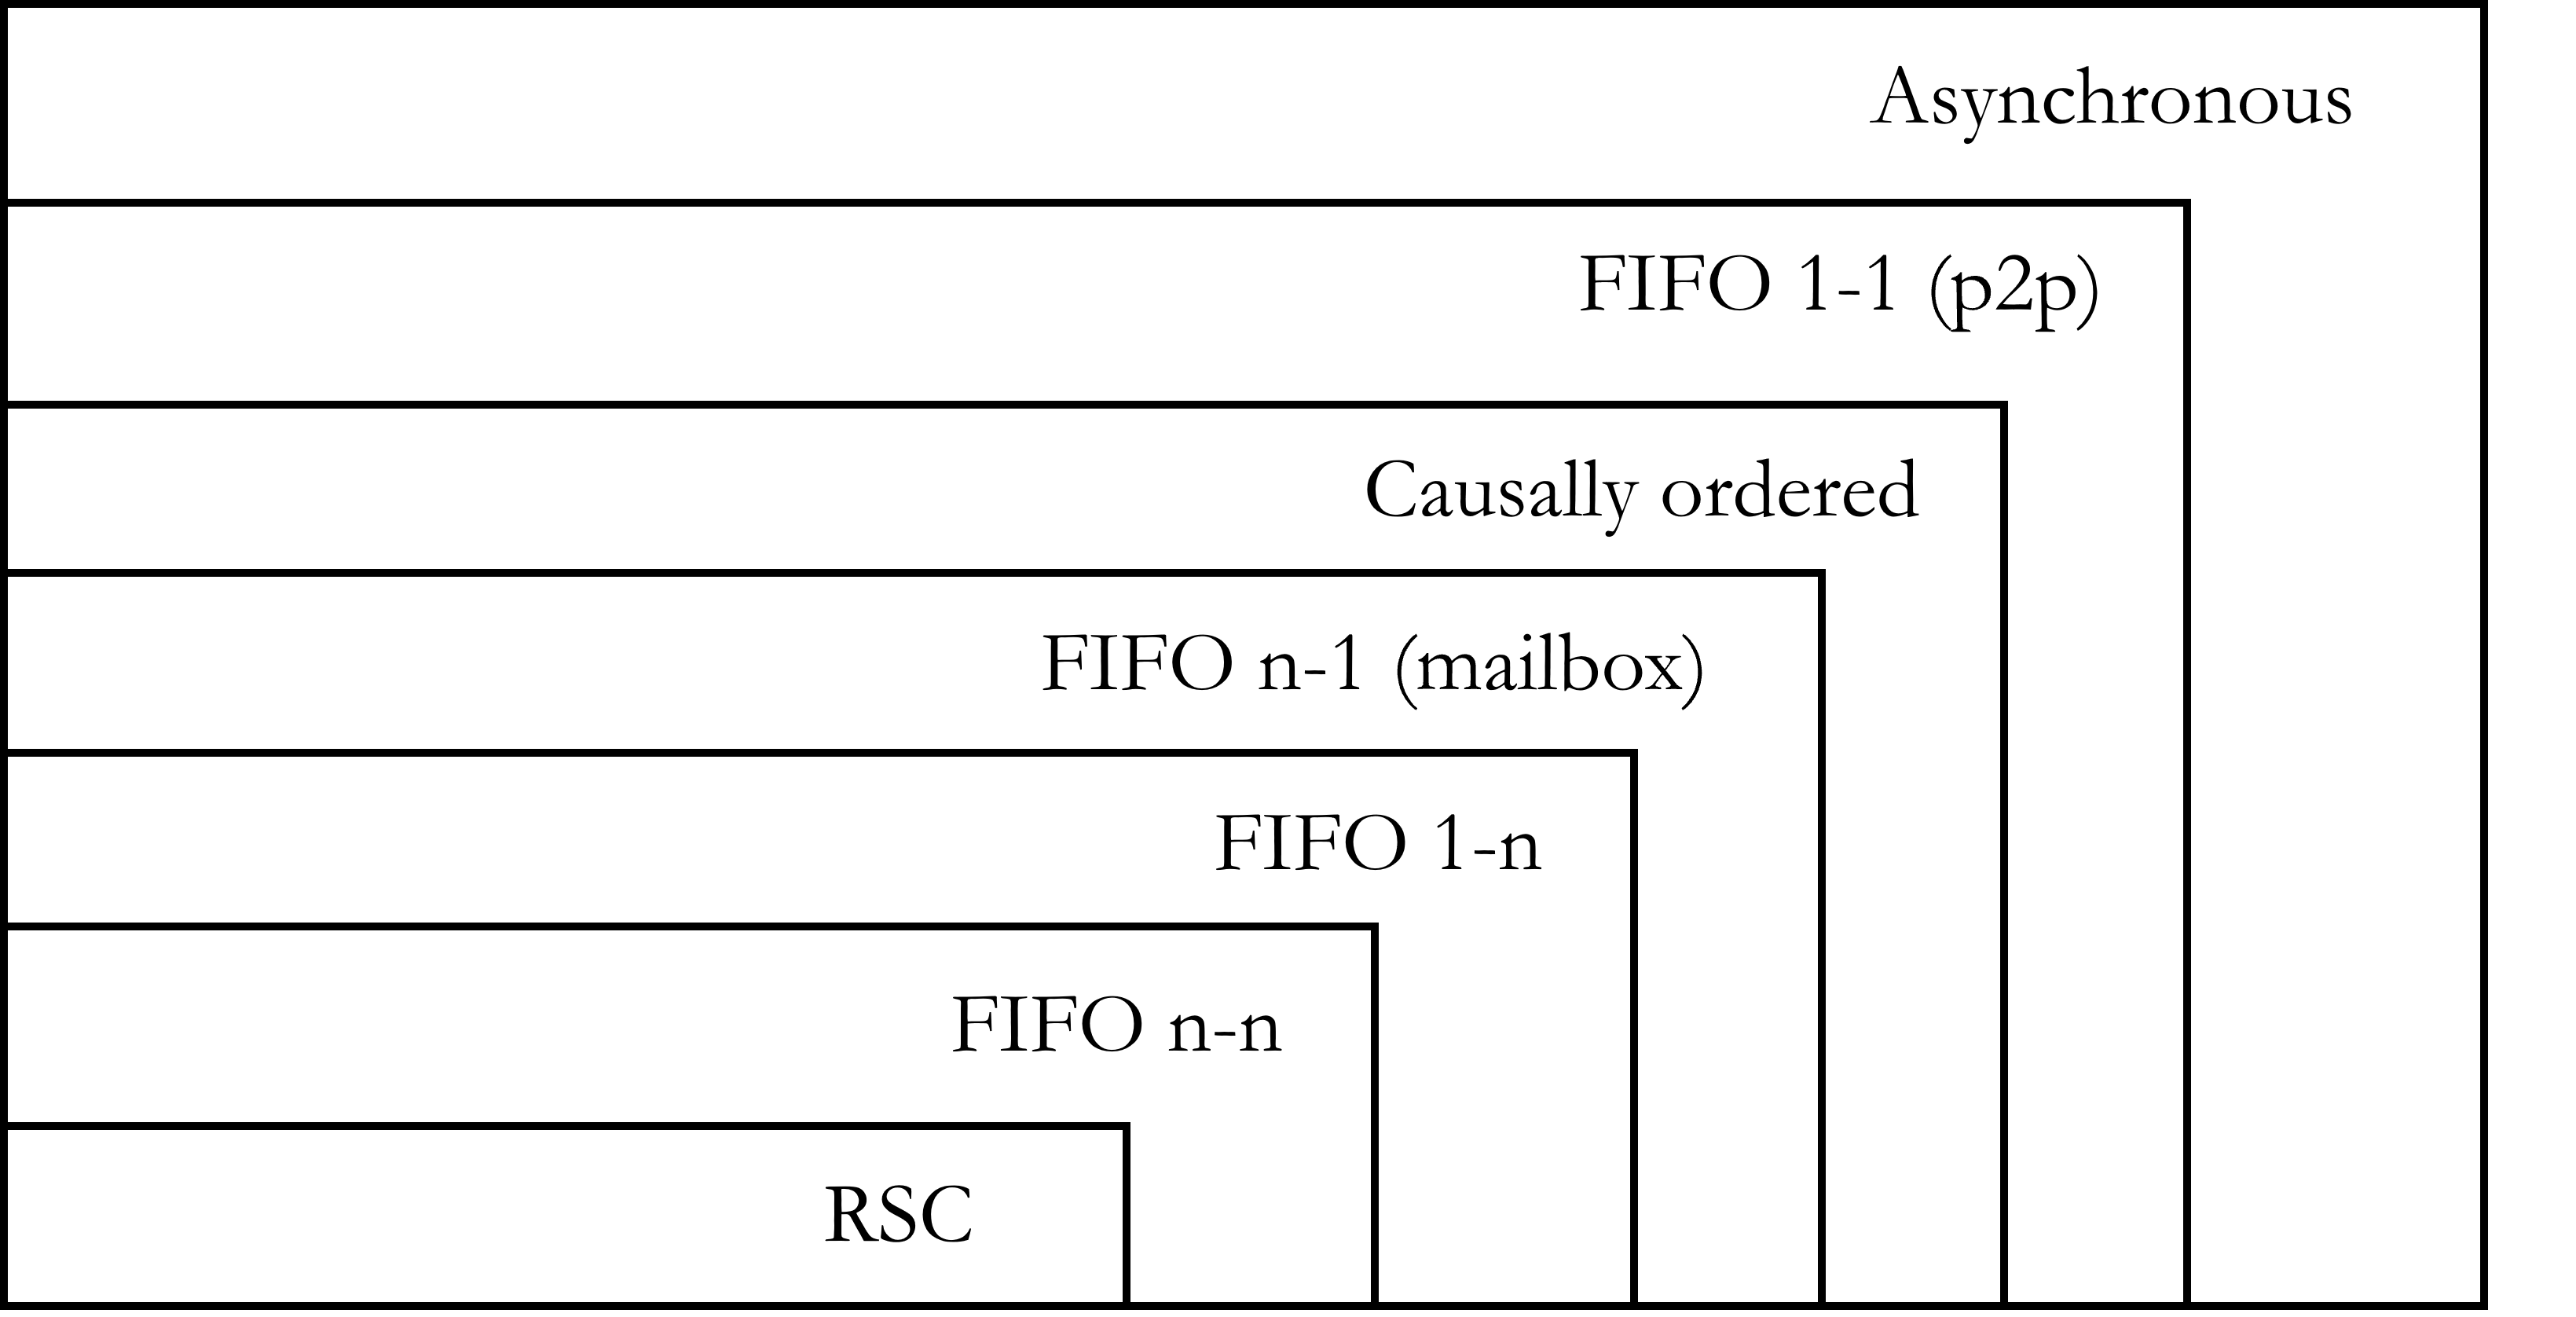
\includegraphics[width=8cm]{msc_hierarchy}
	\caption{The hierarchy of MSC classes.}
	% \label{fig:msc_hierarchy}
\end{figure}

\subsection{Monadic Second-Order Logic}

The set of MSO formulas over (asynchronous) MSCs (over $\Procs$ and $\Msg$) is given by the grammar
$
\phi ::= true \mid x \procrel y \mid x \lhd y \mid \lambda(x) = a \mid x = y \mid x \in X \mid \exists x.\phi \mid \exists X.\phi \mid \phi \vee \phi \mid \neg \phi
$,
where $a \in \Act$, $x$ and $y$ are first-order variables, interpreted as
events of an MSC, and $X$ is a second-order variable, interpreted
as a set of events. We assume that we have an infinite supply of variables,
and we use common abbreviations such as $\wedge$, $\Rightarrow$, $\forall$, etc.
The satisfaction relation is defined in the standard way and self-explanatory.
For example, the formula $\neg\exists x.(\bigvee_{a \in \sAct} \lambda(x) = a \;\wedge\; \neg \mathit{matched}(x))$
with $\mathit{matched}(x) = \exists y.x \lhd y$
says that there are no unmatched send events.
It is not satisfied by  MSC $\mscweakuniver$
of Fig.~\ref{fig:msc_weak_univer},
as message $\msg_1$ is not received,
but by $\mscstrongexist$ from Fig.~\ref{fig:msc_strong_exist}.

Given a sentence $\phi$, i.e., a formula without free variables,
we let $L(\phi)$ denote the set of MSCs that satisfy $\phi$. Since we have defined the set of MSO formulas over asynchronous MSCs, the formula $\asformula = true$ clearly describes the set of asynchronous MSCs, i.e. $L(\asformula) = \asMSCs$. It is worth mentioning that the (reflexive) transitive closure of a binary relation defined by an MSO formula\footnote{See Section~\ref{sec:mso_extra} for details.} with free variables $x$ and $y$, such as $x \procrel y$, is MSO-definable so that the logic can freely use formulas of the form $x \procrel^+ y$, $x \procrel^* y$ or $x \le y$ (where $\le$ is interpreted as $\le$ for the given MSC $\msc$).

\paragraph*{Peer-to-peer MSCs}
	The set of \pp MSCs is MSO-definable as
	\[
		\ppformula = \neg \exists s.\exists s'. \left(
		\bigvee_{\substack{p \in \Procs, q \in \Procs}}\;
		\bigvee_{\substack{a,b \in \pqsAct{p}{q}}}\hspace{-1em}
		(\lambda(s) = a \;\wedge\; \lambda(s') = b) \;\wedge\; s \procrel^+ s' \;\wedge\;
		(\psi_1 \vee \psi_2 )
		\right)
	\]
	where $\psi_1$ and $\psi_2$ are
	\[
		\psi_1 = \exists r.\exists r'.\left(
		\begin{array}{ll}
			s \lhd r & \wedge\\
			s' \lhd r' & \wedge\\
			r' \procrel^+ r &
		\end{array}
		\right) \quad \quad
		\psi_2 = (\neg \mathit{matched}(s) \wedge \mathit{matched}(s'))
		\]
		\[
		matched(x) = \exists y. x \lhd y
	\]

The property $\ppformula$ says that there cannot be two matched send events $s$ and $s'$, with the same sender and receiver, such that either
\begin{enumerate*}[label={(\roman*)}]
	\item $s \procrel^+ s'$ and their receipts happen in the reverse order, or
	\item $s$ is unmatched and $s'$ is matched.
\end{enumerate*}
In other words, it ensures that channels operate in FIFO mode, where an unmatched messages blocks the receipt of all the subsequent messages on that channel.
The set $\ppMSCs$ is therefore MSO-definable as $\ppMSCs=L(\ppformula)$.

\paragraph*{Causally ordered MSCs}
Given an MSC $\msc$, it is causally ordered if and only if it satisfies the MSO formula
\[
	\coformula = \neg \exists s.\exists s'. \left(
	\bigvee_{\substack{q \in \Procs}}\;
	\bigvee_{\substack{a,b \in \pqsAct{\plh}{q}}}\hspace{-1em}
	(\lambda(s) = a \;\wedge\; \lambda(s') = b) \;\wedge\; s \le s' \;\wedge\;
	(\psi_1 \vee \psi_2 )
	\right)
\]
where $\psi_1$ and $\psi_2$ are the same formulas used for \pp.

The property $\coformula$ says that there cannot be two send events $s$ and $s'$, with the same recipient, such that $s \le s'$ and either
\begin{enumerate*}[label={(\roman*)}]
	\item their corresponding receive events $r$ and $r'$ happen in the opposite order, i.e. $r' \procrel^+ r$, or
	\item $s$ is unmatched and $s'$ is matched.
\end{enumerate*}
The set $\coMSCs$ of causally ordered MSCs is therefore MSO-definable as $\coMSCs=L(\coformula)$.

\paragraph*{Mailbox MSCs}

Given an MSC $\msc$, it is a mailbox MSC if and only if it satisfies the MSO formula
\[
	\mbformula = \ppformula \;\wedge\; \neg \exists x.\exists y.(\neg (x = y) \wedge x \mbpartial y \wedge y \mbpartial x)
\]
The set $\mbMSCs$ of mailbox MSCs is therefore MSO-definable as $\mbMSCs=L(\mbformula)$.
\davide{This does not match my definition of mailbox MSC, should I also give the alternative definition (the one in the concur paper) or rewrite everything according to my definition? Give both definitions and prove that they are equivalent}

\paragraph*{$\onen$ MSCs}

Following Definition~\ref{def:one_n_alt}, an MSC $\msc$ is a $\onen$ MSC if and only if it satisfies the MSO formula
\[
	\onenformula = \neg \exists x.\exists y.(\neg (x = y) \wedge x \onenpartial y \wedge y \onenpartial x)
\]
Recall that $\onenpartial$ is the union of the MSO-definable relations $\procrel$, $\lhd$, and $\onenrel$. In particular, we can define $x \onenrel y$ as
\[
x \onenrel y =
\begin{array}{rl}
& \left(
	\bigvee_{\substack{p \in \Procs\\a,b \in \psAct{p}}}\hspace{-1em}
	(\lambda(x) = a \;\wedge\; \lambda(y) = b)
	\;\wedge\; \mathit{matched}(x) \;\wedge\; \neg \mathit{matched}(y)
\right) \;\vee\\
& \left(
	\bigvee_{\substack{p \in \Procs\\a,b \in \prAct{p}}}\hspace{-1em}
	(\lambda(x) = a \;\wedge\; \lambda(y) = b)
	\;\wedge\;
	\exists x'.\exists y'. (x' \lhd x \;\wedge\; y' \lhd y \;\wedge\; x' \procrel^+ y')
\right)\\
\end{array}
\]
The MSO formula for $x \onenrel y$ closely follows Definition~\ref{def:one_n_alt}. The set $\onenMSCs$ of $\onen$ MSCs is therefore MSO-definable as $\onenMSCs=L(\onenformula)$.

\paragraph*{$\nn$ MSCs}

Following Definition~\ref{def:n_n_alt}, an MSC $\msc$ is a $\nn$ MSC if and only if it satisfies the MSO formula
\[
	\nnformula = \neg \exists x.\exists y.(\neg (x = y) \wedge x \nnbowtieofmsc\msc y \wedge y \nnbowtieofmsc\msc x)
\]
In particular, we can define $x \nnbowtieofmsc\msc y$ as
\[
	x \nnbowtieofmsc\msc y =
	\begin{array}{rl}
	& \left(
		\bigvee_{\substack{a,b \in \psAct{\plh}}}
		(\lambda(x) = a \;\wedge\; \lambda(y) = b)
		\;\wedge\; \mathit{matched}(x) \;\wedge\; \neg \mathit{matched}(y)
	\right) \;\vee\\
	& (x \nnrelofmsc{\msc} y) \quad \vee \quad \psi_3 \quad \vee \quad \psi_4\\
	\end{array}
\]

\noindent where $\psi_3$ and $\psi_4$ are defined as
\[
	\psi_3 =
	\begin{array}{rl}
		& \bigvee_{\substack{a,b \in \prAct{\plh}}}
		  (\lambda(x) = a \;\wedge\; \lambda(y) = b)
		  \;\wedge\; \\
		& \exists x'.\exists y'.(x' \lhd x \;\wedge\; y' \lhd y) \;\wedge\; (x' \nnrelofmsc{\msc} y') \;\wedge\; \neg(x \nnrelofmsc{\msc} y)\\
	\end{array}
\]
\[
	\psi_4 =
	\begin{array}{rl}
		& \bigvee_{\substack{a,b \in \psAct{\plh}}}
		  (\lambda(x) = a \;\wedge\; \lambda(y) = b)
		  \;\wedge\; \\
		& \exists x'.\exists y'.(x \lhd x' \;\wedge\; y \lhd y') \;\wedge\; (x' \nnrelofmsc{\msc} y') \;\wedge\; \neg(x \nnrelofmsc{\msc} y)\\
	\end{array}
\]

The MSO formula for $x \nnrelofmsc{\msc} y$ closely follows Definition~\ref{def:n_n_alt}. The set $\nnMSCs$ of $\nn$ MSCs is therefore MSO-definable as $\nnMSCs=L(\nnformula)$.

\paragraph*{$\rsc$ MSCs}

Following Definition~\ref{def:rsc_alt}, an MSC $\msc$ is a $\rsc$ MSC if and only if it satisfies the MSO formula
\[
\Phi_{\rsc} = \neg \exists s_1.\exists s_2. s_1 \varpropto s_2 \;\wedge\; s_2 \varpropto^\ast s_1
\]
\noindent where $\varpropto$ is defined as
\[
s_1 \varpropto s_2 =
\bigvee_{\substack{e \in \sAct}}(\lambda(s_1) = e) \;\wedge\;
s_1 \neq s_2 \;\wedge\;
\exists r_2. (s_1 < r_2 \;\wedge\; s_2 \lhd r_2)
\]
% \davidequestion{The following formula should be wrong... I cannot use $n$ in an MSO formula}
% \[
% 	\rscformula =
% 	\begin{array}{rl}
% 		& \forall x.\left(\bigvee_{a \in \psAct{\plh}} \lambda(x) = a \;\implies\; \mathit{matched}(x)\right) \;\wedge\; \\
% 		& \neg \left(
% 			\bigvee_{k=1}^n \left(
% 			\exists s_1 \cdots s_k. \exists r_1 \cdots r_k.
% 			\bigwedge_{i=1}^k (s_i \lhd r_i \;\wedge\; s_i \le r_{(i+1)\%k})
% 		\right)
% 		\right)\\
% 	\end{array}
% \]
% where $n$ is the total number of messages. The formula checks that there are no unmatched send events and that in the conflict graph there is no cycle, of any length, whose edges are all SR.

\fi
\end{document}
